\chapter{Dòng điện và mạch dao động điện từ}

\begin{vd}[Lò xo dẫn điện]
Chiều dài của cuộn dây lò xo (như trong hình) có $N$ vòng, bán kính $R$, chiều dài ban đầu $x_0$ và độ cứng $k$, sẽ thay đổi như thế nào khi một dòng điện $I_0$ chạy trong nó?
\begin{center}


\tikzset{every picture/.style={line width=0.75pt}} %set default line width to 0.75pt        

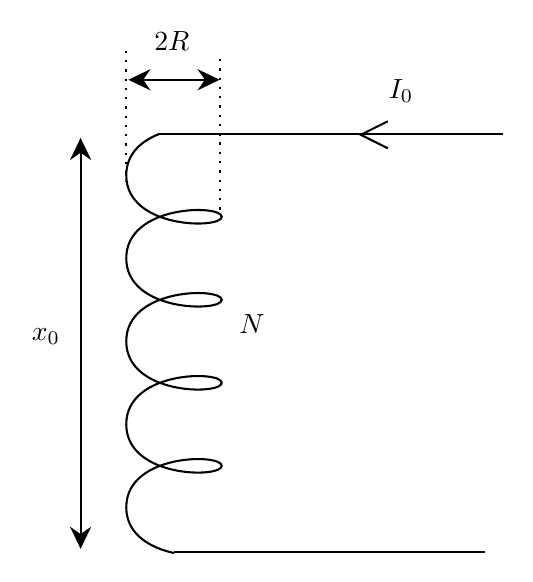
\begin{tikzpicture}[x=0.75pt,y=0.75pt,yscale=-1,xscale=1]
%uncomment if require: \path (0,407); %set diagram left start at 0, and has height of 407

%Shape: Spring [id:dp7981156470236961] 
\draw   (145,297) .. controls (133.5,294.5) and (122,288) .. (122,275) .. controls (122,249) and (168,249) .. (168,255) .. controls (168,261) and (122,261) .. (122,235) .. controls (122,209) and (168,209) .. (168,215) .. controls (168,221) and (122,221) .. (122,195) .. controls (122,169) and (168,169) .. (168,175) .. controls (168,181) and (122,181) .. (122,155) .. controls (122,129) and (168,129) .. (168,135) .. controls (168,141) and (122,141) .. (122,115) .. controls (122,104.6) and (129.36,98.36) .. (138.19,95) ;
%Straight Lines [id:da01655637717315339] 
\draw    (137.67,95) -- (303.67,95) ;
%Straight Lines [id:da857350119897883] 
\draw    (145,296.67) -- (295,296.67) ;
\draw   (248,89) -- (235,95.5) -- (248,102) ;
%Straight Lines [id:da14600989105470585] 
\draw  [dash pattern={on 0.84pt off 2.51pt}]  (122,55) -- (122,118) ;
%Straight Lines [id:da9964300557007086] 
\draw  [dash pattern={on 0.84pt off 2.51pt}]  (167,59) -- (167,134) ;
%Straight Lines [id:da5022542103388066] 
\draw    (126,69) -- (164,69) ;
\draw [shift={(167,69)}, rotate = 180] [fill={rgb, 255:red, 0; green, 0; blue, 0 }  ][line width=0.08]  [draw opacity=0] (10.72,-5.15) -- (0,0) -- (10.72,5.15) -- (7.12,0) -- cycle    ;
\draw [shift={(123,69)}, rotate = 0] [fill={rgb, 255:red, 0; green, 0; blue, 0 }  ][line width=0.08]  [draw opacity=0] (10.72,-5.15) -- (0,0) -- (10.72,5.15) -- (7.12,0) -- cycle    ;
%Straight Lines [id:da9323732479959266] 
\draw    (100,100) -- (100,292) ;
\draw [shift={(100,295)}, rotate = 270] [fill={rgb, 255:red, 0; green, 0; blue, 0 }  ][line width=0.08]  [draw opacity=0] (10.72,-5.15) -- (0,0) -- (10.72,5.15) -- (7.12,0) -- cycle    ;
\draw [shift={(100,97)}, rotate = 90] [fill={rgb, 255:red, 0; green, 0; blue, 0 }  ][line width=0.08]  [draw opacity=0] (10.72,-5.15) -- (0,0) -- (10.72,5.15) -- (7.12,0) -- cycle    ;

% Text Node
\draw (134,44.4) node [anchor=north west][inner sep=0.75pt]    {$2R$};
% Text Node
\draw (75,187.4) node [anchor=north west][inner sep=0.75pt]    {$x_{0}$};
% Text Node
\draw (175,180.4) node [anchor=north west][inner sep=0.75pt]    {$N$};
% Text Node
\draw (247,67.4) node [anchor=north west][inner sep=0.75pt]    {$I_{0}$};


\end{tikzpicture}

\end{center}
\end{vd}
\begin{loigiai}\[\]
Hãy tưởng tượng rằng dòng điện $I_0$ chạy trong một cuộn dây siêu dẫn bị nối tắt, có $N$ vòng, tiết diện $ A=\pi{R^2}$ và chiều dài $x_0$. Độ lớn cảm ứng từ bên trong cuộn dây khi đó là $ B=\dfrac{\mu_0IN}{x_0}$ và tổng từ thông $\Phi=BAN=\dfrac{\mu_0I_0N^2A}{x_0}$. Kể cả khi chiều dài cuộn dây thay đổi vì một lí do nào đó, từ thông bên trong vẫn không đổi, vì nếu có, sẽ gây ra một suất điện động cảm ứng và sinh ra một dòng điện lớn vô cùng do điện trở cuộn dây là $0$. Thế nên dòng điện phải thay đổi theo $x$ là $I(x)=I_0\dfrac{x}{x_0}$ . Độ tự cảm của cuộn dây dài x là $ L(x)=\dfrac{\mu_0N^2A}{x}$, và năng lượng từ trường của cuộn dây có dòng $I$ chạy trong nó là:
$${W}_t=\dfrac{1}{2}L{I^2}=\mu_0\dfrac{N^2I_0^2A}{2x_0^2}x.$$
Như vậy, năng lượng cuộn dây tỉ lệ thuận với $x$, tức ${W}_m(x)\propto x$ . Hệ số tỉ lệ $F_0$ chính là lực co lại gây bởi từ trường, vì một công ${W}=F_0x$ cần tác dụng để kéo giãn cuộn dây ra một chiều dài $x$.\\
Cuộn dây sẽ đạt trạng thái cân bằng khi lực co lại của từ trường cân bằng với lực đàn hồi $ F(x)=k\left(x_0-x\right)$, tức là khi chiều dài cuộn dây thay đổi một khoảng:
$$\Delta x=x_0-x=\dfrac{F_0}{k}\approx{\mu_0}\dfrac{\pi I_0^2N^2R^2}{2kx_0^2}.$$
\end{loigiai}


\begin{vd}[Nam châm và diode]
Một vòng dây kín hình tròn bán kính $r$ được làm từ dây dẫn có bán kính $R$ và một diode, cả hai linh kiện này được coi là lý tưởng. Vòng dây được giữ trong mặt phẳng nằm ngang, và một chiếc ống dài bằng thủy tinh dài đi qua tâm của vòng như hình vẽ. Tìm tổng điện tích đi qua diode nếu chúng ta thả rơi một nam châm có moment từ $m$ đi qua ống.
\end{vd}
\begin{loigiai}\[\]
    Từ thông đi qua vòng dây, tạo ra bởi thanh nam châm thay đổi trong quá trình rơi. Như vậy theo định luật Faraday, trong vòng dây xuất hiện suất điện động cảm ứng:
    \[V^*=-\dfrac{\mathrm{d}\Phi}{\mathrm{d}t}.\]
    Trong quá trình rơi, suất điện động gây ra bởi vòng dây có thể theo bất kì chiều nào tùy theo sự biến thiên của từ thông, do đó diode có thể chặ4n dòng (mạch biến thành mạch hở) hoặc cho dòng điện đi qua tự do (như một dây dẫn).
    \begin{center}
        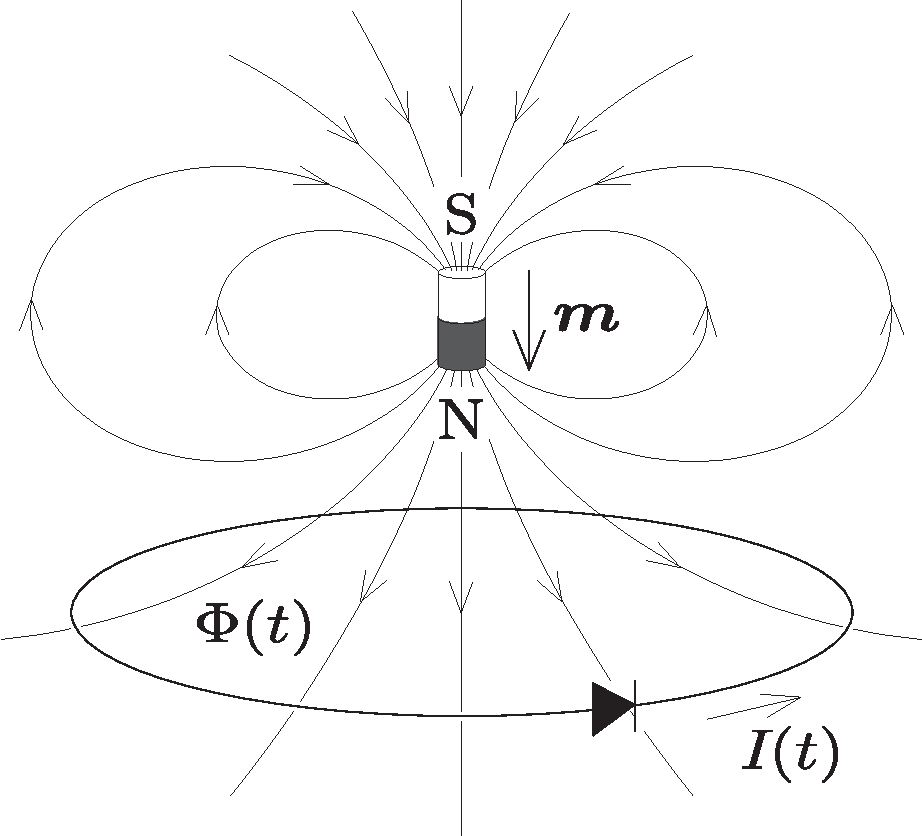
\includegraphics[scale=0.4]{Anh/Nam3.pdf}
    \end{center}
    Độ lớn của từ thông đi qua vòng, bắt đầu ở giá trị gần như bằng không và tăng dần khi nam châm vào gần vòng và cuối cùng đạt cực đại khi nam châm ở vị trí chính giữa vòng; sau đó khi nam châm vượt qua vòng thì từ thông sẽ giảm dần. Áp dụng định luật Lenz ta có thể thấy rằng ở chuyển động đầu tiên, dòng điện sẽ có xu hướng đi qua diode theo chiều dẫn điện do đó sẽ có điện tích đi qua diode. Sau đó khi nam châm rời xa vòng dây, chiều suất điện động đổi hướng và do đó lúc này diode sẽ không cho dòng điện đi qua nữa, do đó không có dòng điện chạy qua vòng ở nửa sau của chuyển động.
    \\Với diode mở, cường độ dòng điện chạy qua nó có thể tính theo định luật Ohm:
    \[\dfrac{\mathrm{d}\Phi}{\mathrm{d}t}=R\dfrac{\mathrm{d}Q}{\mathrm{d}t}.\]
    Sự xuất hiện của dấu $*$ trong biểu thức của suất điện động là do nó phụ thuộc vào chiều dòng điện chạy qua vòng dây, từ đây ta có:
    \[\dfrac{\mathrm{d}\left(\Phi -RQ\right)}{\mathrm{d}t}=0
    \rt \Phi(t)-RQ(t)=\const.\]
    Ban đầu, từ thông qua vòng là không đáng kể và dòng điện chạy qua vòng bằng không nên giá trị của hằng số ở đây cũng bằng không. Dòng điện chỉ đi qua diode đến khi từ thông qua vòng đạt giá trị cực đại, sau đó diode sẽ chặn không cho dòng đi qua nữa. Do đó tổng điện tích đi qua vòng dây trong quá trình đó là:
    \[Q=\dfrac{\Phi_{max}}{R}.\]
    Việc còn lại của chúng ta là tính từ thông đi qua vòng dây lúc nam châm ở chính giữa vòng dây. Để đơn giản, ta thay nam châm bằng một vòng dây bán kính $r_0$ có dòng điện $I_0$, với $r_0$ được chọn sao cho moment từ của vòng dây đúng bằng $m$. Ta có:
    \[\left|\Vec{m}\right|=\pi r_o^2I_0.\]
    Ta dễ dàng chứng minh được công thức độ hỗ cảm của hai vòng dây đặt chồng lên nhau là: 
    \[M=\dfrac{\mu_0 \pi r_0^2}{2r}.\]
    Do đó từ thông cực đại đi qua vòng dây, được tạo ra khi nam châm ở tâm của vòng dây là:
    \[\Phi_{max}=MI_0=\dfrac{\mu_0 \pi r_0^2}{2r}I_0=\dfrac{\mu_0 \left|\Vec{m}\right|}{2r}.\]
    Cuối cùng, tổng điện tích đi qua diode là:
    \[Q=\dfrac{\mu_0 \left|\Vec{m}\right|}{2rR}.\]
\end{loigiai}


\begin{vd}[Hiệu ứng do điện trở suất không đồng nhất]
Hai hình trụ dẫn điện có hình dạng giống hệt nhau, đều có chiều cao $h$ và bán kính $a$ nhưng có điện trở suất khác nhau là $\rho_1$ và $\rho_2$. Hai hình trụ được mắc nối tiếp với nhau như trên hình vẽ, tạo thành một hình trụ dẫn điện duy nhất có chiều cao $2h$ và tiết diện mặt cắt $S=\pi a^2$. Hai đáy đối diện của hình trụ được nối với một nguồn điện để cung cấp một hiệu điện thế không đổi $V$ cho hệ (xem hình vẽ).
  \begin{center}
\tikzset{every picture/.style={line width=0.75pt}} %set default line width to 0.75pt        

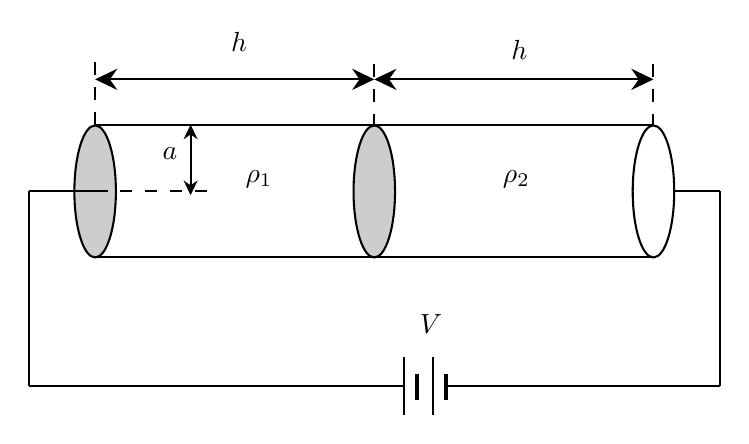
\begin{tikzpicture}[x=0.75pt,y=0.75pt,yscale=-1,xscale=1]
%uncomment if require: \path (0,300); %set diagram left start at 0, and has height of 300

%Shape: Ellipse [id:dp6121391228854065] 
\draw  [fill={rgb, 255:red, 155; green, 155; blue, 155 }  ,fill opacity=0.5 ] (108,92.8) .. controls (108,75.24) and (112.48,61) .. (118,61) .. controls (123.52,61) and (128,75.24) .. (128,92.8) .. controls (128,110.36) and (123.52,124.6) .. (118,124.6) .. controls (112.48,124.6) and (108,110.36) .. (108,92.8) -- cycle ;
%Straight Lines [id:da4868766515682539] 
\draw    (118,61) -- (229,61) -- (387,61) ;
%Shape: Ellipse [id:dp23551700839825673] 
\draw  [fill={rgb, 255:red, 155; green, 155; blue, 155 }  ,fill opacity=0.5 ] (242.5,92.8) .. controls (242.5,75.24) and (246.98,61) .. (252.5,61) .. controls (258.02,61) and (262.5,75.24) .. (262.5,92.8) .. controls (262.5,110.36) and (258.02,124.6) .. (252.5,124.6) .. controls (246.98,124.6) and (242.5,110.36) .. (242.5,92.8) -- cycle ;
%Shape: Ellipse [id:dp6488234880094885] 
\draw   (377,92.8) .. controls (377,75.24) and (381.48,61) .. (387,61) .. controls (392.52,61) and (397,75.24) .. (397,92.8) .. controls (397,110.36) and (392.52,124.6) .. (387,124.6) .. controls (381.48,124.6) and (377,110.36) .. (377,92.8) -- cycle ;
%Straight Lines [id:da8103537955913243] 
\draw    (118,124.6) -- (387,124.6) ;
%Straight Lines [id:da5376961085936793] 
\draw    (118,92.8) -- (86,92.8) ;
%Straight Lines [id:da9455654270816132] 
\draw    (419,92.8) -- (397,92.8) ;
%Straight Lines [id:da6282627412057236] 
\draw    (86,92.8) -- (86,186.6) ;
%Straight Lines [id:da7621747934473055] 
\draw    (86,186.6) -- (267,186.6) ;
%Straight Lines [id:da8771997109727767] 
\draw    (419,92.8) -- (419,186.6) ;
%Straight Lines [id:da3736616951165468] 
\draw    (288,186.6) -- (419,186.6) ;
%Straight Lines [id:da2248812348878848] 
\draw    (121,38.8) -- (249.5,38.8) ;
\draw [shift={(252.5,38.8)}, rotate = 180] [fill={rgb, 255:red, 0; green, 0; blue, 0 }  ][line width=0.08]  [draw opacity=0] (10.72,-5.15) -- (0,0) -- (10.72,5.15) -- (7.12,0) -- cycle    ;
\draw [shift={(118,38.8)}, rotate = 0] [fill={rgb, 255:red, 0; green, 0; blue, 0 }  ][line width=0.08]  [draw opacity=0] (10.72,-5.15) -- (0,0) -- (10.72,5.15) -- (7.12,0) -- cycle    ;
%Straight Lines [id:da8663420360267051] 
\draw    (255.5,38.8) -- (384,38.8) ;
\draw [shift={(387,38.8)}, rotate = 180] [fill={rgb, 255:red, 0; green, 0; blue, 0 }  ][line width=0.08]  [draw opacity=0] (10.72,-5.15) -- (0,0) -- (10.72,5.15) -- (7.12,0) -- cycle    ;
\draw [shift={(252.5,38.8)}, rotate = 0] [fill={rgb, 255:red, 0; green, 0; blue, 0 }  ][line width=0.08]  [draw opacity=0] (10.72,-5.15) -- (0,0) -- (10.72,5.15) -- (7.12,0) -- cycle    ;
%Straight Lines [id:da9871661779176883] 
\draw  [dash pattern={on 4.5pt off 4.5pt}]  (118,92.8) -- (173,92.8) ;
%Straight Lines [id:da14706230389773922] 
\draw    (164,63.6) -- (164,91.6) ;
\draw [shift={(164,94.6)}, rotate = 270] [fill={rgb, 255:red, 0; green, 0; blue, 0 }  ][line width=0.08]  [draw opacity=0] (7.14,-3.43) -- (0,0) -- (7.14,3.43) -- (4.74,0) -- cycle    ;
\draw [shift={(164,60.6)}, rotate = 90] [fill={rgb, 255:red, 0; green, 0; blue, 0 }  ][line width=0.08]  [draw opacity=0] (7.14,-3.43) -- (0,0) -- (7.14,3.43) -- (4.74,0) -- cycle    ;
%Straight Lines [id:da3610058452350251] 
\draw    (267,172.8) -- (267,200.4) ;
%Straight Lines [id:da8374418838314643] 
\draw [line width=1.5]    (273,180.6) -- (273,193.4) ;
%Straight Lines [id:da279996133245511] 
\draw    (281,172.8) -- (281,200.4) ;
%Straight Lines [id:da8399458261151034] 
\draw [line width=1.5]    (287,180.6) -- (287,193.4) ;
%Straight Lines [id:da823848516819623] 
\draw  [dash pattern={on 4.5pt off 4.5pt}]  (118,30.6) -- (118,61) ;
%Straight Lines [id:da6692601063799626] 
\draw  [dash pattern={on 4.5pt off 4.5pt}]  (252.5,31.6) -- (252.5,61) ;
%Straight Lines [id:da6206478957645265] 
\draw  [dash pattern={on 4.5pt off 4.5pt}]  (387,31.6) -- (387,61) ;


% Text Node
\draw (149,70.4) node [anchor=north west][inner sep=0.75pt]    {$a$};
% Text Node
\draw (182,14.4) node [anchor=north west][inner sep=0.75pt]    {$h$};
% Text Node
\draw (317,18.4) node [anchor=north west][inner sep=0.75pt]    {$h$};
% Text Node
\draw (189,81.4) node [anchor=north west][inner sep=0.75pt]    {$\rho _{1}$};
% Text Node
\draw (313,81.4) node [anchor=north west][inner sep=0.75pt]    {$\rho _{2}$};
% Text Node
\draw (273,150.4) node [anchor=north west][inner sep=0.75pt]    {$V$};


\end{tikzpicture}
\end{center}

 \begin{enumerate}[1)]
    \item Tìm cường độ điện trường, dòng điện và mật độ dòng điện chạy trong hai hình trụ ở điều kiện ổn định.
   \item Tìm mật độ điện mặt tại hai đáy nối với nguồn của hình trụ và tại mặt giao cắt của hai loại vật liệu.
 \end{enumerate}
 \end{vd}
 
 \begin{loigiai}\[\]
\begin{enumerate}
  \item Chúng ta sử dụng hệ tọa độ trụ $(r,\phi,z)$, với trục $z$ trùng với trục dối xứng của hai hình trụ, và gốc tọa độ $O$ nằm trên mặt phân cách của hai hình trụ (xem hình vẽ). Chúng ta đặt mật độ điện tích khối là $q_v$, do kí hiệu $\rho$ đã được dùng đại diện cho điện trở suất. Trong trạng thái dừng ta phải có $\partial_t q_v =0$ ở toàn không gian nếu không điện tích khối sẽ liên tục tăng hoặc liên tục giảm đến thời gian vô cùng.
  
  \immini{Do đó, áp dụng phương trình liên tục, ta có:
        \[ \nabla \cdot \ot{J} = -\partial_t q_v =0 . \tag{1} \]

Mặt khác, từ $\nabla \cdot \ot{E} = 4\pi k_e q_v$ và $\ot{J} = \ot{E}/\rho$ chúng ta thu được:
      \[ 0= \nabla \cdot \ot{J} = \frac{1}{\rho} \nabla \cdot \ot{E} = \frac{4\pi k_e }{\rho} q_v, \tag {2} \]

chứng tỏ rằng mật độ điện tích khối $q_v$ phải bằng không trên toàn không gian bên trong vật dẫn ở điều kiện dừng. Tuy nhiên ở bề mặt tiếp xúc giữa hai hình trụ vẫn tồn tại tích điện bề mặt.}{
  
\tikzset{every picture/.style={line width=0.75pt}} %set default line width to 0.75pt        

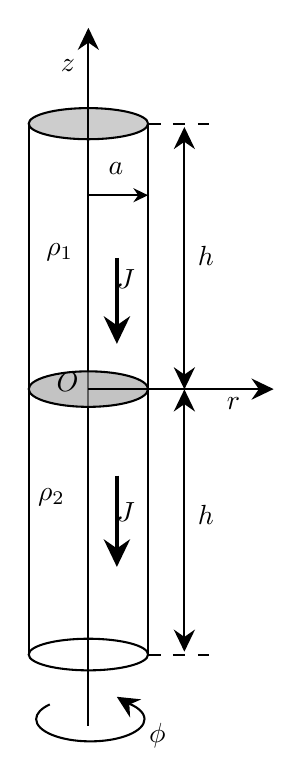
\begin{tikzpicture}[x=0.75pt,y=0.75pt,yscale=-1,xscale=1]
%uncomment if require: \path (0,513); %set diagram left start at 0, and has height of 513

%Shape: Ellipse [id:dp6250624101115241] 
\draw  [fill={rgb, 255:red, 155; green, 155; blue, 155 }  ,fill opacity=0.5 ] (259,53.99) .. controls (259,49.85) and (271.87,46.49) .. (287.75,46.49) .. controls (303.63,46.49) and (316.5,49.85) .. (316.5,53.99) .. controls (316.5,58.13) and (303.63,61.49) .. (287.75,61.49) .. controls (271.87,61.49) and (259,58.13) .. (259,53.99) -- cycle ;
%Straight Lines [id:da3339667292579327] 
\draw    (287.75,10.8) -- (287.75,344.31) ;
\draw [shift={(287.75,7.8)}, rotate = 90] [fill={rgb, 255:red, 0; green, 0; blue, 0 }  ][line width=0.08]  [draw opacity=0] (10.72,-5.15) -- (0,0) -- (10.72,5.15) -- (7.12,0) -- cycle    ;
%Shape: Ellipse [id:dp3305378714078062] 
\draw  [fill={rgb, 255:red, 155; green, 155; blue, 155 }  ,fill opacity=0.6 ] (259,181.88) .. controls (259,177.15) and (271.87,173.32) .. (287.75,173.32) .. controls (303.63,173.32) and (316.5,177.15) .. (316.5,181.88) .. controls (316.5,186.6) and (303.63,190.43) .. (287.75,190.43) .. controls (271.87,190.43) and (259,186.6) .. (259,181.88) -- cycle ;
%Shape: Ellipse [id:dp3007741333558356] 
\draw   (259,309.77) .. controls (259,305.56) and (271.87,302.15) .. (287.75,302.15) .. controls (303.63,302.15) and (316.5,305.56) .. (316.5,309.77) .. controls (316.5,313.97) and (303.63,317.38) .. (287.75,317.38) .. controls (271.87,317.38) and (259,313.97) .. (259,309.77) -- cycle ;
%Straight Lines [id:da7991380491110527] 
\draw    (259,53.99) -- (259,309.77) ;
%Straight Lines [id:da04582733466088573] 
\draw    (316.5,53.99) -- (316.5,309.77) ;
%Straight Lines [id:da469953626106149] 
\draw    (287.75,181.88) -- (374,181.88) ;
\draw [shift={(377,181.88)}, rotate = 180] [fill={rgb, 255:red, 0; green, 0; blue, 0 }  ][line width=0.08]  [draw opacity=0] (10.72,-5.15) -- (0,0) -- (10.72,5.15) -- (7.12,0) -- cycle    ;
%Straight Lines [id:da18645827300171325] 
\draw  [dash pattern={on 4.5pt off 4.5pt}]  (316.5,53.99) -- (345.69,53.99) ;
%Straight Lines [id:da7137054061751509] 
\draw  [dash pattern={on 4.5pt off 4.5pt}]  (316.5,309.77) -- (345.69,309.77) ;
%Straight Lines [id:da32063934724277665] 
\draw    (287.75,88.47) -- (313.5,88.47) ;
\draw [shift={(316.5,88.47)}, rotate = 180] [fill={rgb, 255:red, 0; green, 0; blue, 0 }  ][line width=0.08]  [draw opacity=0] (7.14,-3.43) -- (0,0) -- (7.14,3.43) -- (4.74,0) -- cycle    ;
%Straight Lines [id:da5545535578117207] 
\draw [line width=1.5]    (301.48,118.6) -- (301.48,156.06) ;
\draw [shift={(301.48,160.06)}, rotate = 270] [fill={rgb, 255:red, 0; green, 0; blue, 0 }  ][line width=0.08]  [draw opacity=0] (13.4,-6.43) -- (0,0) -- (13.4,6.44) -- (8.9,0) -- cycle    ;
%Straight Lines [id:da5189897246868762] 
\draw [line width=1.5]    (301.48,223.6) -- (301.48,263.54) ;
\draw [shift={(301.48,267.54)}, rotate = 270] [fill={rgb, 255:red, 0; green, 0; blue, 0 }  ][line width=0.08]  [draw opacity=0] (13.4,-6.43) -- (0,0) -- (13.4,6.44) -- (8.9,0) -- cycle    ;
%Shape: Arc [id:dp2351818332087896] 
\draw  [draw opacity=0] (305.74,332.79) .. controls (311.28,334.75) and (314.79,337.65) .. (314.79,340.89) .. controls (314.79,346.81) and (303.1,351.6) .. (288.68,351.6) .. controls (274.27,351.6) and (262.58,346.81) .. (262.58,340.89) .. controls (262.58,338.17) and (265.07,335.68) .. (269.16,333.79) -- (288.68,340.89) -- cycle ; \draw   (305.74,332.79) .. controls (311.28,334.75) and (314.79,337.65) .. (314.79,340.89) .. controls (314.79,346.81) and (303.1,351.6) .. (288.68,351.6) .. controls (274.27,351.6) and (262.58,346.81) .. (262.58,340.89) .. controls (262.58,338.17) and (265.07,335.68) .. (269.16,333.79) ;
%Straight Lines [id:da29136919346471224] 
\draw    (305.74,332.79) -- (303.97,331.7) ;
\draw [shift={(301.42,330.12)}, rotate = 391.63] [fill={rgb, 255:red, 0; green, 0; blue, 0 }  ][line width=0.08]  [draw opacity=0] (10.72,-5.15) -- (0,0) -- (10.72,5.15) -- (7.12,0) -- cycle    ;
%Straight Lines [id:da8801372758814372] 
\draw    (334,58.6) -- (334,179) ;
\draw [shift={(334,182)}, rotate = 270] [fill={rgb, 255:red, 0; green, 0; blue, 0 }  ][line width=0.08]  [draw opacity=0] (10.72,-5.15) -- (0,0) -- (10.72,5.15) -- (7.12,0) -- cycle    ;
\draw [shift={(334,55.6)}, rotate = 90] [fill={rgb, 255:red, 0; green, 0; blue, 0 }  ][line width=0.08]  [draw opacity=0] (10.72,-5.15) -- (0,0) -- (10.72,5.15) -- (7.12,0) -- cycle    ;
%Straight Lines [id:da7076307678955314] 
\draw    (334,185) -- (334,305.4) ;
\draw [shift={(334,308.4)}, rotate = 270] [fill={rgb, 255:red, 0; green, 0; blue, 0 }  ][line width=0.08]  [draw opacity=0] (10.72,-5.15) -- (0,0) -- (10.72,5.15) -- (7.12,0) -- cycle    ;
\draw [shift={(334,182)}, rotate = 90] [fill={rgb, 255:red, 0; green, 0; blue, 0 }  ][line width=0.08]  [draw opacity=0] (10.72,-5.15) -- (0,0) -- (10.72,5.15) -- (7.12,0) -- cycle    ;


% Text Node
\draw (315.5,341.2) node [anchor=north west][inner sep=0.75pt]    {$\phi $};
% Text Node
\draw (262,228.4) node [anchor=north west][inner sep=0.75pt]    {$\rho _{2}$};
% Text Node
\draw (266,110.4) node [anchor=north west][inner sep=0.75pt]    {$\rho _{1}$};
% Text Node
\draw (300,123) node [anchor=north west][inner sep=0.75pt]  {$\ot{J}$};
% Text Node
\draw (300,235.12) node [anchor=north west][inner sep=0.75pt]    {$\ot{J}$};
% Text Node
\draw (271,172.4) node [anchor=north west][inner sep=0.75pt]    {$O$};
% Text Node
\draw (353,184.4) node [anchor=north west][inner sep=0.75pt]    {$r$};
% Text Node
\draw (339,111.4) node [anchor=north west][inner sep=0.75pt]    {$h$};
% Text Node
\draw (339,236.4) node [anchor=north west][inner sep=0.75pt]    {$h$};
% Text Node
\draw (296,71.4) node [anchor=north west][inner sep=0.75pt]    {$a$};
% Text Node
\draw (273,21.4) node [anchor=north west][inner sep=0.75pt]    {$z$};


\end{tikzpicture}}
Nếu chúng ta giả sử rằng $h \gg a$, kết hợp với $\nabla\cdot \ot{J}=0$ và $\nabla \times \ot{E}=0$, ta suy ra mật độ dòng $\ot{J}$ là đồng nhất trên toàn bộ hình trụ, có chiều hướng xuống dọc theo trục $z$. Do $\ot{E}$ và $\ot{J}$ là tỉ lệ thuận với nhau bên trong mỗi hình trụ nên ta dễ dàng suy ra $\ot{E}$ là đồng nhất trong từng hình trụ riêng biệt. Mật độ dòng $\ot{J}$ phải liên tục khi đi qua mặt phân cách của hai hình trụ nếu không điện tích sẽ tích tụ đến vô hạn trên mặt phân cách này. Do đó, mật độ dòng $\ot{J}$ là không đổi trên toàn bộ vật dẫn, và cường độ dòng điện là $I= J\pi a^2$.\\
Điện trở của từng hình trụ $R_{1,2}$ lần lượt là:
   \[R_{1,2} = \rho_{1,2} \frac{h}{\pi a^2} , \tag{3} \]

Dẫn đến tổng trở của vật dẫn:
    \[R = R_1 + R_2 = (\rho_1 + \rho_2 ) \frac{h}{\pi a^2}. \tag{4} \]

Dòng điện và mật độ dòng điện chạy trong hệ là:
    \[I = \frac{V}{R} = \frac{\pi a^2 V }{h(\rho_1 + \rho_2)}, \quad J = \frac{V}{h(\rho_1 + \rho_2)}. \tag{5} \]

Vì chúng ta có cùng mật độ dòng điện trên hai hình trụ có điện trở suất khác nhau và $\ot{E} = \rho \ot{J}$, điện trường bên trong từng hình trụ phải là khác nhau, chúng ta đặt là:
   \[ E_1 = \rho_1 J = \frac{\rho_1 V}{h(\rho_1 + \rho_2)} , \quad E_2 =\rho_2 J = \frac{\rho_2 V}{h(\rho_1 + \rho_2)}. \tag{6} \]

\item Mật độ điện tích mặt ở trên mặt phân cách hai hình trụ có thể tính được qua định luật Gauss:
  \[\sigma = \frac{1}{4\pi k_e} (E_2 - E_1) = \frac{1}{4\pi k_e} \frac{(\rho_2 - \rho_1)V}{h(\rho_1 +\rho_2)} . \tag{7} \]

Giả sử rằng, điện trường là bằng không bên ngoài 2 đáy của hình trụ lớn, mật độ điện tích mặt của hai đáy trụ cũng có thể được tính theo định luật Gauss :
  
   \[\sigma_1 = \frac{E_1}{4\pi k_e }= \frac{1}{4\pi k_e} \frac{\rho_1 V}{h(\rho_1 + \rho_2)} , \quad \sigma_2 = - \frac{E_2}{4\pi k_e}= - \frac{1}{4\pi k_e} \frac{\rho_2 V}{h(\rho_1 + \rho_2)} . \tag{8}\]
                 
    
\end{enumerate}
\end{loigiai}


\begin{vd}[Trở kháng vô hạn]
Với dòng điện xoay chiều có tần số góc $\omega$, tìm trở kháng tương đương giữa các cực $A$ và $B$ trên hình vẽ. Mạch vô hạn gồm rất nhiều các phần tử giống hệt nhau, mỗi nút mạng cấu tạo từ một cuộn cảm có độ tự cảm $L$ và một tụ điện có điện dung $C$. Liệu có khả năng trở kháng này có 2 giá trị khác nhau hay không?
\begin{center}
    

\tikzset{every picture/.style={line width=0.75pt}} %set default line width to 0.75pt        

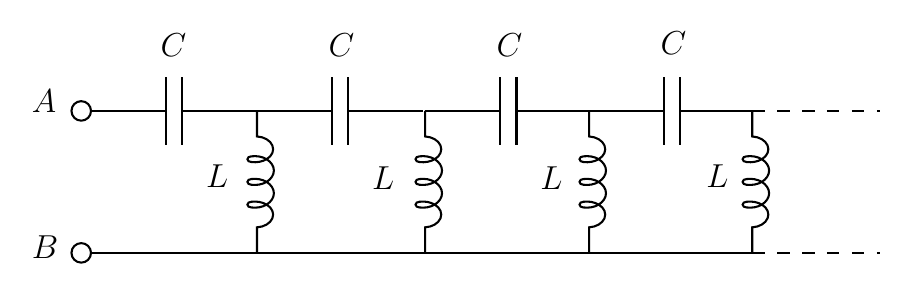
\begin{tikzpicture}[x=0.75pt,y=0.75pt,yscale=-1,xscale=1]
%uncomment if require: \path (0,470); %set diagram left start at 0, and has height of 470

%Straight Lines [id:da8896708259213006] 
\draw    (148,270.4) -- (468,270.4) ;
%Shape: Capacitor [id:dp8244944796033653] 
\draw   (148,202) -- (184,202) (192,185.8) -- (192,218.2) (184,185.8) -- (184,218.2) (192,202) -- (228,202) ;
%Shape: Inductor (Air Core) [id:dp47563115184590754] 
\draw   (466.59,202) -- (466.59,214.31) .. controls (470.02,214.49) and (472.95,216.2) .. (473.97,218.62) .. controls (475,221.04) and (473.91,223.67) .. (471.23,225.26) .. controls (469.14,226.48) and (466.44,226.98) .. (463.81,226.62) .. controls (462.79,226.62) and (461.96,226.01) .. (461.96,225.26) .. controls (461.96,224.5) and (462.79,223.89) .. (463.81,223.89) .. controls (466.44,223.54) and (469.14,224.03) .. (471.23,225.26) .. controls (473.45,226.68) and (474.72,228.66) .. (474.72,230.73) .. controls (474.72,232.8) and (473.45,234.78) .. (471.23,236.2) .. controls (469.14,237.42) and (466.44,237.92) .. (463.81,237.57) .. controls (462.79,237.57) and (461.96,236.96) .. (461.96,236.2) .. controls (461.96,235.44) and (462.79,234.83) .. (463.81,234.83) .. controls (466.44,234.48) and (469.14,234.98) .. (471.23,236.2) .. controls (473.45,237.62) and (474.72,239.6) .. (474.72,241.67) .. controls (474.72,243.74) and (473.45,245.72) .. (471.23,247.14) .. controls (469.14,248.37) and (466.44,248.86) .. (463.81,248.51) .. controls (462.79,248.51) and (461.96,247.9) .. (461.96,247.14) .. controls (461.96,246.39) and (462.79,245.78) .. (463.81,245.78) .. controls (466.44,245.42) and (469.14,245.92) .. (471.23,247.14) .. controls (473.91,248.73) and (475,251.36) .. (473.97,253.78) .. controls (472.95,256.2) and (470.02,257.91) .. (466.59,258.09) -- (466.59,270.4) ;
%Flowchart: Connector [id:dp26467715626009025] 
\draw   (138.6,270.4) .. controls (138.6,273) and (140.7,275.1) .. (143.3,275.1) .. controls (145.9,275.1) and (148,273) .. (148,270.4) .. controls (148,267.8) and (145.9,265.7) .. (143.3,265.7) .. controls (140.7,265.7) and (138.6,267.8) .. (138.6,270.4) -- cycle ;
%Flowchart: Connector [id:dp5760989978301936] 
\draw   (138.6,202) .. controls (138.6,204.6) and (140.7,206.7) .. (143.3,206.7) .. controls (145.9,206.7) and (148,204.6) .. (148,202) .. controls (148,199.4) and (145.9,197.3) .. (143.3,197.3) .. controls (140.7,197.3) and (138.6,199.4) .. (138.6,202) -- cycle ;
%Shape: Inductor (Air Core) [id:dp45982416209467436] 
\draw   (388,202) -- (388,214.31) .. controls (391.43,214.49) and (394.35,216.2) .. (395.38,218.62) .. controls (396.4,221.04) and (395.31,223.67) .. (392.63,225.26) .. controls (390.54,226.48) and (387.84,226.98) .. (385.22,226.62) .. controls (384.2,226.62) and (383.37,226.01) .. (383.37,225.26) .. controls (383.37,224.5) and (384.2,223.89) .. (385.22,223.89) .. controls (387.84,223.54) and (390.54,224.03) .. (392.63,225.26) .. controls (394.86,226.68) and (396.12,228.66) .. (396.12,230.73) .. controls (396.12,232.8) and (394.86,234.78) .. (392.63,236.2) .. controls (390.54,237.42) and (387.84,237.92) .. (385.22,237.57) .. controls (384.2,237.57) and (383.37,236.96) .. (383.37,236.2) .. controls (383.37,235.44) and (384.2,234.83) .. (385.22,234.83) .. controls (387.84,234.48) and (390.54,234.98) .. (392.63,236.2) .. controls (394.86,237.62) and (396.12,239.6) .. (396.12,241.67) .. controls (396.12,243.74) and (394.86,245.72) .. (392.63,247.14) .. controls (390.54,248.37) and (387.84,248.86) .. (385.22,248.51) .. controls (384.2,248.51) and (383.37,247.9) .. (383.37,247.14) .. controls (383.37,246.39) and (384.2,245.78) .. (385.22,245.78) .. controls (387.84,245.42) and (390.54,245.92) .. (392.63,247.14) .. controls (395.31,248.73) and (396.4,251.36) .. (395.38,253.78) .. controls (394.35,256.2) and (391.43,257.91) .. (388,258.09) -- (388,270.4) ;
%Shape: Inductor (Air Core) [id:dp9344396637665358] 
\draw   (309,202) -- (309,214.31) .. controls (312.43,214.49) and (315.35,216.2) .. (316.38,218.62) .. controls (317.4,221.04) and (316.31,223.67) .. (313.63,225.26) .. controls (311.54,226.48) and (308.84,226.98) .. (306.22,226.62) .. controls (305.2,226.62) and (304.37,226.01) .. (304.37,225.26) .. controls (304.37,224.5) and (305.2,223.89) .. (306.22,223.89) .. controls (308.84,223.54) and (311.54,224.03) .. (313.63,225.26) .. controls (315.86,226.68) and (317.12,228.66) .. (317.12,230.73) .. controls (317.12,232.8) and (315.86,234.78) .. (313.63,236.2) .. controls (311.54,237.42) and (308.84,237.92) .. (306.22,237.57) .. controls (305.2,237.57) and (304.37,236.96) .. (304.37,236.2) .. controls (304.37,235.44) and (305.2,234.83) .. (306.22,234.83) .. controls (308.84,234.48) and (311.54,234.98) .. (313.63,236.2) .. controls (315.86,237.62) and (317.12,239.6) .. (317.12,241.67) .. controls (317.12,243.74) and (315.86,245.72) .. (313.63,247.14) .. controls (311.54,248.37) and (308.84,248.86) .. (306.22,248.51) .. controls (305.2,248.51) and (304.37,247.9) .. (304.37,247.14) .. controls (304.37,246.39) and (305.2,245.78) .. (306.22,245.78) .. controls (308.84,245.42) and (311.54,245.92) .. (313.63,247.14) .. controls (316.31,248.73) and (317.4,251.36) .. (316.38,253.78) .. controls (315.35,256.2) and (312.43,257.91) .. (309,258.09) -- (309,270.4) ;
%Shape: Inductor (Air Core) [id:dp6736769932143452] 
\draw   (228,202) -- (228,214.31) .. controls (231.43,214.49) and (234.35,216.2) .. (235.38,218.62) .. controls (236.4,221.04) and (235.31,223.67) .. (232.63,225.26) .. controls (230.54,226.48) and (227.84,226.98) .. (225.22,226.62) .. controls (224.2,226.62) and (223.37,226.01) .. (223.37,225.26) .. controls (223.37,224.5) and (224.2,223.89) .. (225.22,223.89) .. controls (227.84,223.54) and (230.54,224.03) .. (232.63,225.26) .. controls (234.86,226.68) and (236.12,228.66) .. (236.12,230.73) .. controls (236.12,232.8) and (234.86,234.78) .. (232.63,236.2) .. controls (230.54,237.42) and (227.84,237.92) .. (225.22,237.57) .. controls (224.2,237.57) and (223.37,236.96) .. (223.37,236.2) .. controls (223.37,235.44) and (224.2,234.83) .. (225.22,234.83) .. controls (227.84,234.48) and (230.54,234.98) .. (232.63,236.2) .. controls (234.86,237.62) and (236.12,239.6) .. (236.12,241.67) .. controls (236.12,243.74) and (234.86,245.72) .. (232.63,247.14) .. controls (230.54,248.37) and (227.84,248.86) .. (225.22,248.51) .. controls (224.2,248.51) and (223.37,247.9) .. (223.37,247.14) .. controls (223.37,246.39) and (224.2,245.78) .. (225.22,245.78) .. controls (227.84,245.42) and (230.54,245.92) .. (232.63,247.14) .. controls (235.31,248.73) and (236.4,251.36) .. (235.38,253.78) .. controls (234.35,256.2) and (231.43,257.91) .. (228,258.09) -- (228,270.4) ;
%Straight Lines [id:da08162931708808219] 
\draw  [dash pattern={on 4.5pt off 4.5pt}]  (466.59,202) -- (528,202) ;
%Straight Lines [id:da19767708053606436] 
\draw  [dash pattern={on 4.5pt off 4.5pt}]  (466.59,270.4) -- (528,270.4) ;
%Shape: Capacitor [id:dp46965472319429713] 
\draw   (228,202) -- (264,202) (272,185.8) -- (272,218.2) (264,185.8) -- (264,218.2) (272,202) -- (308,202) ;
%Shape: Capacitor [id:dp5547460041167185] 
\draw   (309,202) -- (345,202) (353,185.8) -- (353,218.2) (345,185.8) -- (345,218.2) (353,202) -- (389,202) ;
%Shape: Capacitor [id:dp25623842683890086] 
\draw   (388,202) -- (424,202) (432,185.8) -- (432,218.2) (424,185.8) -- (424,218.2) (432,202) -- (468,202) ;


% Text Node
\draw (180,163.4) node [anchor=north west][inner sep=0.75pt]  [font=\large]  {$C$};
% Text Node
\draw (261,163.4) node [anchor=north west][inner sep=0.75pt]  [font=\large]  {$C$};
% Text Node
\draw (342,163.4) node [anchor=north west][inner sep=0.75pt]  [font=\large]  {$C$};
% Text Node
\draw (421,162.4) node [anchor=north west][inner sep=0.75pt]  [font=\large]  {$C$};
% Text Node
\draw (202,226.4) node [anchor=north west][inner sep=0.75pt]  [font=\large]  {$L$};
% Text Node
\draw (282,227.4) node [anchor=north west][inner sep=0.75pt]  [font=\large]  {$L$};
% Text Node
\draw (363,227.4) node [anchor=north west][inner sep=0.75pt]  [font=\large]  {$L$};
% Text Node
\draw (443,226.4) node [anchor=north west][inner sep=0.75pt]  [font=\large]  {$L$};
% Text Node
\draw (118,190.4) node [anchor=north west][inner sep=0.75pt]  [font=\large]  {$A$};
% Text Node
\draw (118,260.6) node [anchor=north west][inner sep=0.75pt]  [font=\large]  {$B$};


\end{tikzpicture}
\end{center}
\end{vd}
\begin{loigiai}\[\]
Ta có công thức tính trở kháng của cuộn dây khi có dòng điện với tần số $\omega$ đi qua:
$$\dfrac{V_C}{I_C}=\dfrac{1}{\omega C},$$
đây được gọi là dung kháng của cuộn dây, hơn nữa, dòng điện đi qua cuộn dây luôn sớm pha hơn hiệu điện thế xoay chiều đặt lên nó một góc $90^\circ$. Với cuộn dây, tương tự ta có
$$\dfrac{V_L}{I_L}=\omega L,$$
đây được gọi là cảm kháng của cuộn dây, dòng điện qua cuộn dây luôn chậm pha so với hiệu điện thế xoay chiều đặt lên nó một góc $90^\circ.$\\
Do sự lệch pha so với hiệu điện thế của dòng qua cuộn dây và dòng qua tụ điện là hoàn toàn ngược nhau nên ta có thể coi cuộn dây là một tụ điện có điện dung âm $C_L<0$:
$$\omega L=-\dfrac{1}{\omega C_L}, \text{ và do đó } C_L=-\dfrac{1}{\omega^2 L}.$$
Từ đây ta có thể tính toán dựa trên một mạch điện tương đương chỉ gồm toàn tụ điện.
Trong các tính toán tiếp theo, để cho gọn ta đặt :
$$k^2=\dfrac{1}{\omega^2 LC}=\tron{\dfrac{\omega_0}{\omega}}^2.$$
Hệ số tỉ lệ $k$ cho chúng ta biết tần số góc tự nhiên (hay còn gọi là tần số góc cộng hưởng) $\omega_0$ đối với mạch $LC$ đơn thuần lớn hơn bao nhiêu lần so với tần số  góc cưỡng bức $\omega$. Sử dụng rút gọn này, “điện dung hiệu dụng” của cuộn dây có thể viết dưới dạng $C_L=-k^2\cdot C$.\\
Trong một bài vật lý, mạch điện vô hạn có thể được hiểu là mạch điện với số nút mạng vô cùng lớn nhưng số nút mạng là hữu hạn. Đầu tiên hãy xét một mạch điện chứa $n$ nút mạng (mạch chứa $n$ cuộn dây và $n$ tụ điện). Vì mạch điện không có bất kì phần tử điện trở nào nên độ lệch pha giữa dòng điện trong mạch và hiệu điện thế đặt vào hai đầu mạch chỉ có thể là $90^\circ$ hoặc $-90^\circ$. Khi đó, tùy vào độ lệch pha ta có thể thay thế toàn bộ mạch điện bằng một tụ điện tương đương $C_n$ hoặc một cuộn dây tương đương $L_n$ với thông số phù hợp. Giả sử trong trường hợp này mạch điện có thể thay thế bằng một tụ điện $C_n$, ta sẽ tính toán  $C_n$, và nếu $C_n$ âm thì mạch điện tương đương sẽ là một cuộn dây.\\
Trong trường hợp $n=1$, ta sẽ thu được điện dung tương đương của một tụ điện $C$ mắc với một cuộn cảm $L$ (được coi như một tụ điện với điện dung $C_L$ bằng công thức sau:
$$\dfrac{1}{C_1}=\dfrac{1}{C}+\dfrac{1}{C_L},$$
từ đó suy ra:
$$C_{1}=\dfrac{C C_{L}}{C+C_{L}}=\dfrac{C \times\left(-k^{2} C\right)}{C+\left(-k^{2} C\right)}=\dfrac{k^{2}}{k^{2}-1} C .$$
Với $n=2$, mạch điện giống như tụ $C_1$ được mắc với thêm một nút mạng nữa
$$\dfrac{1}{C_2}=\dfrac{1}{C}+\dfrac{1}{C_1+\tron{-k^2 C}}.$$
Tổng quát,
$$\dfrac{1}{C_{n+1}}=\dfrac{1}{C}+\dfrac{1}{C_{n}-k^{2} C},$$
từ đây
$$C_{n+1}=\dfrac{C\left(C_{n}-k^{2} C\right)}{C_{n}+\left(1-k^{2}\right) C}.$$
Để thuận tiện hơn ta đặt $C_n=x_n\cdot C$ vì dãy truy hồi cho $x$ có thể được viết ở dạng tường minh:
\[x_{n+1}=\dfrac{x_n-k^2}{x_n +1 -k^2}.\tag{1} \label{n1}\]
Để khảo sát xem dãy này có giới hạn khi $x$ tiến đến vô cùng hay không, chúng ta giả sử $n\gg 1$ thì $x_n\approx x_{n+1}$, lúc này (\ref{n1}) có thể được chuyển thành một phương trình bậc hai như sau:
$$x=\dfrac{x-k^2}{x+1-k^2}, \text{ hay } x^2-k^2x+k^2=0.$$
Trong trường hợp $k>2$ (tần số đầu vào là nhỏ), phương trình này có hai nghiệm thật:
\[x_{\pm}=\dfrac{k^{2}}{2} \pm \dfrac{k}{2} \sqrt{k^{2}-4}\tag{2}.\label{n2}\]
Câu hỏi được đặt ra là đâu là nghiệm được chọn? Hay cả hai nghiệm đều có ý nghĩa vật lý của riêng chúng? Bạn có thể đoán rằng trong trường hợp này nghiệm nhỏ hơn là nghiệm đúng. Suy đoán trên có cơ sở bởi vì nếu ta dùng cuộn dây có $L$ rất nhỏ thì mỗi cuộn dây chỉ đơn thuần như một dây dẫn nối tắt, vì thế điện dung đo được giữa hai đầu $A B$ sẽ xấp xỉ điện dung của một tụ điện thuần $C$, $x\approx1$. Điều này dễ dàng được kiểm chứng vì khi $L$ là nhỏ, $k\gg 1$, lúc này $x_{-}\approx1$ còn $x_+$ xấp xỉ $k^2 \gg 1$, một điều vô lý so với điều kiện biên vật lý. Vậy đúng như suy đoán, ta chọn nghiệm nhỏ hơn.\\
Lập luận này khẳng định đối với $k>2$, trở kháng của mạch có thể được mô tả bởi công thức 
$$Z_{\text{chuỗi}}=\dfrac{1}{\omega x_{-} C}=\dfrac{1}{\omega C} \dfrac{2}{k\left(k-\sqrt{k^{2}-4}\right)}=\dfrac{1+\sqrt{1-4 \omega^{2} L C}}{2 \omega C}.$$
Vậy nếu $k<2$, điều gì sẽ xảy ra?\\
Lúc này, phương trình (\ref{n1}) sẽ cho nghiệm phức, tức điện dung tương đương sẽ không còn là một bội số thực của $C$. Nói theo một cách khác, lúc này điện dung tương đương của mạch điện sẽ không hội tụ về một giá trị cụ thể mà sẽ phụ thuộc vào số nút mạng (vì trên thực tế số nút mạng chỉ là rất nhiều chứ không phải là vô hạn!).\\
\textbf{Mở rộng.}\\
Bài toán cũng có thể được giải quyết bằng cách đặt trở kháng phức với $i\omega L$ cho cuộn dây và $\dfrac{1}{i\omega C}$ cho tụ điện. Đặt $Z$ là trở kháng của cả mạch điện, nếu mạch điện là vô hạn thì khi ta lắp thêm một nút mạng vào mạch điện thì trở kháng của mạch không thay đổi và bằng $Z$, ta có
$$Z=\dfrac{1}{i\omega C}+\dfrac{i\omega LZ}{i\omega L +Z}.$$
Và ta thu được nghiệm:
$$2Z\sqrt{\dfrac{C}{L}}=-ik\pm \sqrt{4-k^2}.$$
Biểu thức này chứng tỏ, với $k>2$, $Z$ luôn là một số ảo mang dấu âm và coi như một tụ điện trên thực tế.\\
Với $k<2$, thành phần thứ hai của biểu thức là một số thực và trở kháng của mạch vô hạn lúc này chứa một thành phần điện trở. Điều này rất khó hiểu bởi một mạch điện chỉ chứa cuộn cảm và tụ điện lí tưởng không thể coi như một điện trở (vì điện trở làm mất mát năng lượng) do đó nên lẽ ra trở kháng tương đương chỉ có thể coi như một tụ điện hoặc một cuộn cảm.\\
Sự xuất hiện của thành phần điện trở có liên hệ mật thiết đến hiện tượng sóng truyền trong dây dẫn. Sóng này sẽ mang năng lượng của nguồn và truyền đi dọc theo dây dẫn, và trong trường hợp dây dẫn rất dài, sóng sẽ phản xạ và mang năng lượng trở lại sau một khoảng thời gian khá lâu. Đối với trường hợp dây dẫn dài vô hạn, sóng năng lượng này không bao giờ trở lại, do đó mạch điện chỉ gồm cuộn dây và tụ điện lý tưởng sẽ coi như có thêm thành phần điện trở!
\end{loigiai}


\begin{vd}[Truyền tải điện đi xa]\\%câu 12
%USAPhO 2011
Một dây cáp dẫn điện xoay chiều, truyền tải điện năng dưới dạng sóng hình sin với tần số $60~\mathrm{Hz}$. Tải nhận hiệu điện thế có giá trị hiệu dụng là $500~\mathrm{kV}$ và yêu cầu công suất trung bình là $1000~\mathrm{MW}$. Đối với bài này, chỉ xét dây cáp mang dòng điện theo một trong hai hướng, và bỏ qua hiệu ứng do điện dung hoặc độ tự cảm giữa dây tải với đất.
\begin{enumerate}[1.]
    \item Giả sử tải của đường dây điện là một khu dân cư, được coi như một điện trở thuần.
    \begin{enumerate}[a.]
        \item Hãy tính cường độ dòng điện hiệu dụng của đường dây tải điện.
        \item Dây cáp có đường kính $3~\mathrm{cm}$, dài $500~\mathrm{km}$, và được làm bằng nhôm với điện trở suất $2,8\times10^{-8}\mathrm{\Omega\cdot m}$. Hỏi công suất hao phí trên dây là bao nhiêu?
    \end{enumerate}
    \item Một chủ trang trại địa phương nghĩ rằng anh ta có thể lấy điện từ đường dây bằng cách sử dụng cảm ứng điện từ. Chủ trang trại dựng $N$ vòng dây hình chữ nhật có chiều dài $a$ và chiều rộng $b<a$. Một cạnh của vòng được đặt trên mặt đất, dây dẫn thẳng và chạy song song với mặt đất ở độ cao $h$ nhỏ hơn chiều dài của dây rất nhiều. Viết cường độ dòng điện trong dây dưới dạng $I=I_0\sin \omega t$, và giả sử rằng dây trở lại ở rất xa.
    \begin{enumerate}[a.]
        \item Xác định biểu thức cảm ứng từ của từ trường ở khoảng cách $r$ so với dây dẫn điện, biểu diễn kết quả theo $I, r$, và các hằng số cơ bản.
        \item Nên đặt vòng ở đâu, và định hướng chiếc vòng như thế nào, để tối đa hóa suất điện động cảm ứng của nó?
        \item Giả sử vòng được đặt theo cách này, hãy xác định biểu thức của suất điện động cảm ứng của vòng (như một hàm của thời gian) theo $I_0, h, a, b, N, \omega, t$, và các hằng số cơ bản.
        \item Giả sử rằng $a=5~\mathrm{m}, b=2~\mathrm{m}$ và $h=100~\mathrm{m}$. Hỏi người chủ trang trại $N$ bằng bao nhiêu vòng dây để tạo ra một suất điện động cảm ứng hiệu dụng bằng $120~\mathrm{V}$?
    \end{enumerate}
    \item Tải ở cuối của đường dây điện thay đổi, bao gồm một nhà máy sản xuất với số lượng lớn động cơ điện. Trong khi công suất trung bình được giữ không đổi, giờ đây nó hoạt động như một điện trở mắc song song với một cuộn cảm $0,25~\mathrm{H}$.
    \begin{enumerate}[a.]
        \item Công suất hao phí trên đường dây tải điện sẽ tăng lên, giảm đi hay giữ nguyên? (Bạn không cần tính toán giá trị một cách rõ ràng, bạn chỉ cần lập luận để bảo vệ câu trả lời của mình).
        \item Công ty điện lực muốn cho tải hoạt động như ban đầu bằng cách lắp một tụ điện song song với tải. Hỏi điện dung của nó là bao nhiêu?
    \end{enumerate}
\end{enumerate}
\end{vd}
\begin{loigiai}
\begin{enumerate}[1.]
    \item 
    \begin{enumerate}[a.]
        \item Vì tải là điện trở thuần, nên công suất trung bình đơn giản là:
        $$P=I_\mathrm{rms}V_\mathrm{rms},$$
        do đó:
        $$I_\mathrm{rms}=\dfrac{P}{V_\mathrm{rms}}=2000~\mathrm{A}.$$
        \item Diện tích tiết diện của dây là $A=\pi r^2=7,07\times 10^{-4}~\mathrm{m^2}$, do đó điện trở của dây là:
        $$R=\dfrac{\rho L}{A}=19,8 ~\mathrm{\Omega}.$$
        Công suất hao phí:
        $$P=I^2 R=79,2 ~\mathrm{MW}.$$
    \end{enumerate}
    \item
    \begin{enumerate}[a)]
        \item Từ trường vuông góc với dây và bán kính, nên từ định luật Ampere:
        $$
\oint \mathbf{B} \cdot \mathrm{d} \mathbf{s}=\mu_{0} I.$$
Tích phân có giá trị là $\tron{2\pi r}B$, do đó:
$$B=\dfrac{\mu_0 I}{2\pi r}.$$
Kết quả nổi tiếng này cũng có thể được viết ra mà không cần giải thích.
 \item Suất điện động cảm ứng tỉ lệ với tốc độ biến thiên của từ thông qua vòng dây. Vì sự phụ thuộc vào thời gian của từ trường là đều trong không gian, nên tốc độ biến thiên từ thông đạt cực đại khi chính từ thông đạt cực đại. Điều này có thể thực hiện bằng cách tối đa hóa từ trường trong vòng dây và đảm bảo rằng điều đó bình thường đối với vòng. Vì từ trường mạnh hơn khi gần dây, nên vòng dây phải nằm ngay bên dưới dây, và vì từ trường nằm ngang và vuông góc với dây tại vị trí này, nên vòng dây phải thẳng đứng và song song với dây. Cuối cùng, một lần nữa, vì từ trường càng gần dây càng mạnh, nên cạnh dài của vòng phải thẳng đứng.\\
 Tóm lại, vòng nên được đặt thẳng đứng, song song và ngay dưới dây, với cạnh dài thẳng đứng.
 \item Theo định luật Faraday:
 $$\mathcal{E}=N\dfrac{\mathrm \Phi_B}{\mathrm t},$$
 trong đó chúng tôi đã bỏ dấu, vì điều này không quan trọng, và $\Phi_B$ là từ thông đi qua một vòng. Từ thông:
 $$
\Phi_{B}=\int \mathbf{B} \cdot \mathrm{d}\mathbf{A}=b \int_{h-a}^{h} B(r) \mathrm{d} r,
$$
Trong đó chúng tôi đã chia vòng thành nhiều dải mảnh có bề dày $\mathrm{d}r$ và chiều dài $b$. Thay vào kết quả ở phần a:
$$
\Phi_{B}=b \int_{h-a}^{h} \dfrac{\mu_{0} I}{2 \pi r} \mathrm{d} r=\dfrac{\mu_{0} I b}{2 \pi} \ln \frac{h}{h-a}.
$$
Chỉ có cường độ dòng điện phụ thuộc thời gian:
$$\dfrac{\mathrm{d}I}{\mathrm{t}}=\omega I_0 \cos\omega t.$$
Do đó, ta có:
$$\mathcal{E}=\dfrac{N\mu_0b}{2\pi}\mathrm{ln}\dfrac{h}{h-a}I_0\omega\cos\omega t.$$
\item Giá trị hiệu dụng của $I_0\cos \omega t$ chỉ đơn giản là $I_{rms}$, do đó lấy giá trị hiệu dụng của cả hai vế:
$$\mathcal{E_{\mathrm{rms}}}=\dfrac{N\mu_0b}{2\pi}\ln\dfrac{h}{h-a}I_{\mathrm{rms}} \omega=N\mu_0bf\mathrm{ln}\dfrac{h}{h-a}I_\mathrm{rms},$$
trong đó chúng tôi dùng $f=\omega/2\pi$. Thay số, ta được:
$$\mu_0 bf\mathrm{ln}\dfrac{h}{h-a}I_\mathrm{rms}=0,0155~\mathrm{V},$$
vì vậy số vòng dây cần là:
$$N=7760.$$
    \end{enumerate}
    \item 
    \begin{enumerate}[a.]
        \item Cuộn cảm tạo nên một thành phần mới của dòng điện, thành phần này lệch pha $90^\circ$ với điện áp. Giá trị cường độ dòng điện hiệu dụng tăng, do đó công suất hao phí trên dây dẫn cũng tăng lên. Điều này có thể biểu diễn qua trở kháng phức. Định luật Ohm cho ta:
        $$V=IZ,$$
        trong đó cả $V$ và $I$ đều là số phức, và pha tương đối giữa chúng cho ta pha tương đối giữa điện áp và dòng điện. Bỏ qua độ tự cảm, $Z=R$. Với cuộn dây tự cảm, hai trở kháng mắc song song:
        $$Z=\tron{\dfrac{1}{R}}+\dfrac{1}{i\omega L}^{-1}.$$
        Khi $\left|Z\right|$ giảm và $V$ vẫn giữ nguyên, $\left|I\right|$ tăng, như đã lập luận ở trên.
        \item Phương pháp đơn giản nhất là sử dụng các trở kháng phức. Ta muốn triệt tiêu thành phần ảo gây ra bởi cuộn cảm, nên ta cần:
        $$\dfrac{1}{i\omega L}+i\omega C=0,$$
        vì chúng mắc song song. Điều này tương đương với:
        $$\omega=\dfrac{1}{\sqrt{LC}},$$
        do đó
        $$C=\dfrac{1}{\omega^2 L}=28,1 ~\mathrm{\mu F}.$$
        Cũng có thể đưa đến kết quả này mà không cần dùng trở kháng phức. Không cần dòng điện ngoài để mạch $LC$ dao động với tần số riêng, dòng điện chỉ đơn giản chạy qua lại giữa cuộn cảm và tụ điện, mà không cần đi qua nguồn. Do đó, nếu tần số của nguồn phù hợp với tần số riêng của mạch $LC$ thì mạch $LC$ sẽ không ảnh hưởng đến dòng điện trong dây tải, tải hoạt động như không có mạch $LC$ nào cả. Điều này dẫn tới điều kiện $\omega=1/\sqrt{LC}$ như trên.
    \end{enumerate}
\end{enumerate}
\end{loigiai}


\begin{vd}[Mạch $LC$ vô hạn]

\immini{
Khi sóng dao động điện hình $\sin$ lan truyền qua mạng gồm vô
số mạch $LC$. Pha của điện áp trên hai tụ điện liên tiếp chênh lệch nhau một góc $\varphi$.}
{

\tikzset{every picture/.style={line width=0.75pt}} %set default line width to 0.75pt        

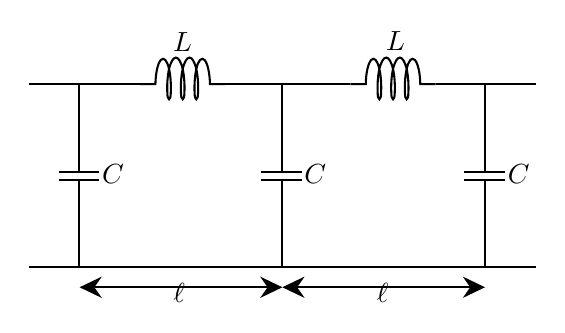
\begin{tikzpicture}[x=0.75pt,y=0.75pt,yscale=-1,xscale=1]
%uncomment if require: \path (0,472); %set diagram left start at 0, and has height of 472

%Shape: Inductor (Air Core) [id:dp7045280265063458] 
\draw   (149.21,82.81) -- (156.6,82.81) .. controls (156.71,77.41) and (157.74,72.8) .. (159.19,71.19) .. controls (160.64,69.58) and (162.22,71.29) .. (163.17,75.51) .. controls (163.91,78.8) and (164.2,83.05) .. (163.99,87.18) .. controls (163.99,88.79) and (163.63,90.1) .. (163.17,90.1) .. controls (162.72,90.1) and (162.35,88.79) .. (162.35,87.18) .. controls (162.14,83.05) and (162.44,78.8) .. (163.17,75.51) .. controls (164.03,72) and (165.21,70.02) .. (166.46,70.02) .. controls (167.7,70.02) and (168.89,72) .. (169.74,75.51) .. controls (170.47,78.8) and (170.77,83.05) .. (170.56,87.18) .. controls (170.56,88.79) and (170.19,90.1) .. (169.74,90.1) .. controls (169.29,90.1) and (168.92,88.79) .. (168.92,87.18) .. controls (168.71,83.05) and (169.01,78.8) .. (169.74,75.51) .. controls (170.59,72) and (171.78,70.02) .. (173.03,70.02) .. controls (174.27,70.02) and (175.46,72) .. (176.31,75.51) .. controls (177.04,78.8) and (177.34,83.05) .. (177.13,87.18) .. controls (177.13,88.79) and (176.76,90.1) .. (176.31,90.1) .. controls (175.86,90.1) and (175.49,88.79) .. (175.49,87.18) .. controls (175.28,83.05) and (175.58,78.8) .. (176.31,75.51) .. controls (177.26,71.29) and (178.84,69.58) .. (180.3,71.19) .. controls (181.75,72.8) and (182.77,77.41) .. (182.88,82.81) -- (190.27,82.81) ;
%Straight Lines [id:da23102535022173476] 
\draw    (95.66,82.81) -- (149.21,82.81) ;
%Straight Lines [id:da06790234025531028] 
\draw    (119.72,82.83) -- (119.72,107.39) ;
%Shape: Capacitor [id:dp9729891012585667] 
\draw   (119.72,107.39) -- (119.72,124.99) (129.5,128.9) -- (109.95,128.9) (129.5,124.99) -- (109.95,124.99) (119.72,128.9) -- (119.72,146.49) ;
%Straight Lines [id:da20984737567415745] 
\draw    (119.72,146.49) -- (119.72,171.05) ;
%Straight Lines [id:da6439594421380794] 
\draw    (95.56,171.05) -- (340,171.05) ;
%Straight Lines [id:da09818757441099835] 
\draw    (217.48,82.83) -- (217.48,107.39) ;
%Shape: Capacitor [id:dp6208715313286415] 
\draw   (217.48,107.39) -- (217.48,124.99) (227.25,128.9) -- (207.7,128.9) (227.25,124.99) -- (207.7,124.99) (217.48,128.9) -- (217.48,146.49) ;
%Straight Lines [id:da20448192374001373] 
\draw    (217.48,146.49) -- (217.48,171.05) ;
%Shape: Inductor (Air Core) [id:dp028398413950593726] 
\draw   (250.55,82.81) -- (257.94,82.81) .. controls (258.05,77.41) and (259.08,72.8) .. (260.53,71.19) .. controls (261.98,69.58) and (263.56,71.29) .. (264.51,75.51) .. controls (265.25,78.8) and (265.55,83.05) .. (265.33,87.18) .. controls (265.33,88.79) and (264.97,90.1) .. (264.51,90.1) .. controls (264.06,90.1) and (263.69,88.79) .. (263.69,87.18) .. controls (263.48,83.05) and (263.78,78.8) .. (264.51,75.51) .. controls (265.37,72) and (266.55,70.02) .. (267.8,70.02) .. controls (269.04,70.02) and (270.23,72) .. (271.08,75.51) .. controls (271.82,78.8) and (272.11,83.05) .. (271.9,87.18) .. controls (271.9,88.79) and (271.54,90.1) .. (271.08,90.1) .. controls (270.63,90.1) and (270.26,88.79) .. (270.26,87.18) .. controls (270.05,83.05) and (270.35,78.8) .. (271.08,75.51) .. controls (271.94,72) and (273.12,70.02) .. (274.37,70.02) .. controls (275.61,70.02) and (276.8,72) .. (277.65,75.51) .. controls (278.38,78.8) and (278.68,83.05) .. (278.47,87.18) .. controls (278.47,88.79) and (278.1,90.1) .. (277.65,90.1) .. controls (277.2,90.1) and (276.83,88.79) .. (276.83,87.18) .. controls (276.62,83.05) and (276.92,78.8) .. (277.65,75.51) .. controls (278.6,71.29) and (280.18,69.58) .. (281.64,71.19) .. controls (283.09,72.8) and (284.11,77.41) .. (284.22,82.81) -- (291.61,82.81) ;
%Straight Lines [id:da9380035862074394] 
\draw    (190.27,82.81) -- (250.55,82.81) ;
%Straight Lines [id:da4180355779200249] 
\draw    (291.61,82.81) -- (339.95,82.81) ;
%Straight Lines [id:da23055841703957425] 
\draw    (315.24,83.02) -- (315.24,107.58) ;
%Shape: Capacitor [id:dp439348391669399] 
\draw   (315.24,107.58) -- (315.24,125.18) (325.01,129.09) -- (305.46,129.09) (325.01,125.18) -- (305.46,125.18) (315.24,129.09) -- (315.24,146.68) ;
%Straight Lines [id:da285003782968297] 
\draw    (315.24,146.68) -- (315.24,171.24) ;
%Straight Lines [id:da5563040277518165] 
\draw    (123.08,180.68) -- (214.77,180.68) ;
\draw [shift={(217.77,180.68)}, rotate = 180] [fill={rgb, 255:red, 0; green, 0; blue, 0 }  ][line width=0.08]  [draw opacity=0] (10.72,-5.15) -- (0,0) -- (10.72,5.15) -- (7.12,0) -- cycle    ;
\draw [shift={(120.08,180.68)}, rotate = 0] [fill={rgb, 255:red, 0; green, 0; blue, 0 }  ][line width=0.08]  [draw opacity=0] (10.72,-5.15) -- (0,0) -- (10.72,5.15) -- (7.12,0) -- cycle    ;
%Straight Lines [id:da42034647305080663] 
\draw    (220.77,180.68) -- (312.4,180.68) ;
\draw [shift={(315.4,180.68)}, rotate = 180] [fill={rgb, 255:red, 0; green, 0; blue, 0 }  ][line width=0.08]  [draw opacity=0] (10.72,-5.15) -- (0,0) -- (10.72,5.15) -- (7.12,0) -- cycle    ;
\draw [shift={(217.77,180.68)}, rotate = 0] [fill={rgb, 255:red, 0; green, 0; blue, 0 }  ][line width=0.08]  [draw opacity=0] (10.72,-5.15) -- (0,0) -- (10.72,5.15) -- (7.12,0) -- cycle    ;

% Text Node
\draw (163.77,177.31) node [anchor=north west][inner sep=0.75pt]    {$\ell $};
% Text Node
\draw (261.79,177.37) node [anchor=north west][inner sep=0.75pt]    {$\ell $};
% Text Node
\draw (129.43,119.98) node [anchor=north west][inner sep=0.75pt]    {$C$};
% Text Node
\draw (226.86,119.98) node [anchor=north west][inner sep=0.75pt]    {$C$};
% Text Node
\draw (324.95,120.31) node [anchor=north west][inner sep=0.75pt]    {$C$};
% Text Node
\draw (163.66,56.59) node [anchor=north west][inner sep=0.75pt]    {$L$};
% Text Node
\draw (266.22,56.11) node [anchor=north west][inner sep=0.75pt]    {$L$};
\end{tikzpicture}
}
\begin{enumerate}[1)]
    \item Xác định sự phụ thuộc của $\varphi$ vào $L, C$ và $\omega$ (với $\omega$ là tần số góc của sóng $\sin$).
    \item Tính vận tốc truyền sóng, nếu chiều dài mỗi mạch là $\ell$.
    \item Với điều kiện nào thì vận tốc truyền sóng hầu như không phụ thuộc vào $\omega$. Tính vận tốc ấy.
    \item Nêu ra một mô hình cơ học đơn giản tương tự như mạng điện trên, các đại lượng nào tương ứng với nhau và suy ra các phương trình thiết lập cho mô hình ấy.
\end{enumerate}
Cho công thức:
\[\begin{aligned}
\cos a - \cos b &= -2 \sin \dfrac{a+b}{2} \cos \dfrac{a-b}{2}\\
\sin a - \sin b &= 2 \cos \dfrac{a+b}{2} \sin \dfrac{a-b}{2}
\end{aligned}\]
\end{vd}

\begin{loigiai}\[\]
Ta kí hiệu như sau: Trong mắt mạng thứ $n$, dòng điện qua cuộn cảm  và tụ điện là $I_{L_n}$ và $I_{C_n}$; hiệu điện thế giữa hai đầu cuộn cảm và tụ điện là $U_{L_n}$ và $U_{C_n}$.
\begin{enumerate}[1)]
    \item Giả sử chiều dòng điện như hình vẽ. Định luật Kiffchorf về nút và mạng cho ta:
    \[\heva{I_{L_{n-1}} + I_{C_n} - I_{L_{n}} &= 0 \\
    U_{C_{n-1}} + U_{L_{n-1}} - U_{C_n} &= 0 }. \tag{1} \label{q.3.1}\]
    Nếu hiệu điện thế của tụ thứ $n$ là:
    \[U_{C_n} =  U_0 \sin (\omega t + n \varphi). \tag{2} \label{q.3.2}\]
    Do $I_{C}$ sớm pha hơn $U_{C}$ một góc $\dfrac{\pi}{2}$ nên dòng điện qua tụ ấy là:
    \[I_{C_n} = \dfrac{U_0}{Z_C} \sin (\omega t + n \varphi  + \dfrac{\pi}{2}) = \omega C U_0 \cos  (\omega t + n \varphi). \tag{3} \label{q.3.3}\]
    Thay (\ref{q.3.2}) vào (\ref{q.3.1}), ta tìm được hiệu điện thế giữa hai đầu cuộn cảm thứ $n - 1$:
    \begin{align*}
        U_{L_{n-1}} &= U_{C_n} - U_{C_{n-1}} \\
        &=  U_0 \sin (\omega t + n \varphi) - U_0 \sin \tron{\omega t + (n-1) \varphi}\\
        &= 2U_0 \sin \dfrac{\varphi}{2} \cos \tron{\omega t + \dfrac{2n-1}{2} \varphi}.
    \end{align*}
    Do $I_L$ trễ pha hơn $U_L$ góc $\dfrac{\pi}{2}$ nên:
    \begin{align*}
        I_{L_{n-1}} &= 2 \dfrac{U_0}{Z_L} \sin \dfrac{\varphi}{2} \cos \tron{\omega t + \dfrac{2n-1}{2} \varphi - \dfrac{\pi}{2}}\\
        &= \dfrac{2U_0}{\omega L}\sin \dfrac{\varphi}{2} \sin \tron{\omega t + \dfrac{2n-1}{2} \varphi}. \tag{4} \label{q.3.4}
    \end{align*}
    Tương tự, thay $n$ bằng $n+1$, ta suy ra:
    \[I_{L_n} = \dfrac{2U_0}{\omega L}\sin \dfrac{\varphi}{2} \sin \tron{\omega t + \dfrac{2n+1}{2} \varphi}. \tag{5} \label{q.3.5}\]
    Thay (\ref{q.3.3}), (\ref{q.3.4}) và (\ref{q.3.5}) vào (\ref{q.3.1}), ta được:
    \[0 = \omega C U_0 \cos  (\omega t + n \varphi) + \dfrac{2U_0}{\omega L}\sin \dfrac{\varphi}{2} \tron{\sin \tron{\omega t + \dfrac{2n-1}{2} \varphi} - \sin \tron{\omega t + \dfrac{2n+1}{2} \varphi}}. \]
    \[0 = \omega C \cos  (\omega t + n \varphi) - \dfrac{4}{\omega L} \sin^2 \dfrac{\varphi}{2}\cos \tron{\omega t + n \varphi}. \]
    \[\rt \omega C = \dfrac{4}{\omega L}\sin^2 \dfrac{\varphi}{2} \rt \varphi = 2\arcsin \tron{\dfrac{\omega\sqrt{LC}}{2}}. \tag{6}\label{q.3.6}\]
    Với $ 0 \le \omega \le \dfrac{2}{\sqrt{LC}}$.
    \item Gọi $\Delta t$ là thời gian để dao động tiến được thêm một mắt ($\ell$).
    \[\Delta t = \dfrac{\ell}{v} = \dfrac{\varphi}{\omega} \rt v = \dfrac{\omega \ell}{\varphi}. \tag{7}\label{q.3.7}\]
    Thay (\ref{q.3.6}) vào (\ref{q.3.7}), ta tính được vận tốc truyền sóng:
    \[v = \dfrac{\omega \ell}{2\arcsin \tron{\dfrac{\omega\sqrt{LC}}{2}}}.\]
    \item Vận tốc truyền sóng không phụ thuộc vào $\omega$ nếu
    \[\arcsin \tron{\dfrac{\omega\sqrt{LC}}{2}} \propto \omega \quad (\text{tỉ lệ}).\]
    Điều này chỉ đúng với $\omega$ rất nhỏ, kéo theo: $\dfrac{\omega\sqrt{LC}}{2} \ll 1 \rt \omega \ll \dfrac{2}{\sqrt{LC}}$. \\
    Vận tốc truyền sóng lúc này là:
    \[v = \dfrac{\ell}{\sqrt{LC}}.\]
    \item Vì mạng điện không có điện trở hay máy thu nào khác nên năng lượng của mạch được bảo toàn.
    \[W =  \sum_n \dfrac{1}{2} \tron{CU_{C_n}^2 + L I_{L_n}^2}. \tag{8} \label{q.3.8}\]
    Mối quan hệ với cơ học không thể nhận biết được theo cách này vì hai đại lượng vật lý khác nhau $(U_{C_n}$ và $I_{L_n})$ liên quan nhưng không có gì tương ứng với quan hệ giữa tọa độ $x$ và vận tốc $v = \dot{x}$.\\
    Để tạo ra sự tương tự cơ học, năng lượng phải được mô tả dưới dạng điện tích của tụ $Q$ và dòng điện $I = \dot{Q}$ và hằng số $L, C$ tương tự hằng số $k, m$ trong cơ học. Vì vậy, ta cần phải biểu diễn điện áp $U_{C_n}$ theo điện tích $Q_{L_n}$ đi qua cuộn dây.\\
    Từ định luật bảo toàn điện tích:
    \[Q_{L_{n-1}} + Q_{C_n} - Q_{L_n} = 0, \tag{9}\label{q.3.9}\]
    với $Q_L$ là điện tích đi qua cuộn cảm, $Q_C$ là điện tích của tụ. Mặt khác, ta có:
    \[ \heva{U_{C_n} &= \dfrac{Q_{C_n}}{C} \\
    I_{L_n} &= \dot{Q}_{L_n}}.\tag{10}\label{q.3.10} \]
    Từ (\ref{q.3.8}), (\ref{q.3.9}) và (\ref{q.3.10}) suy ra:
    \[W = \sum\limits_n {\left[ {\underbrace {\dfrac{L}{2}\cdot\dot{Q}_{L_n}^{2}}_A + \underbrace {\dfrac{1}{{2 C}}{{\left( {{Q_{{L_n}}} - {Q_{{L_{n - 1}}}}} \right)}^2}}_B} \right]}.\]
    $W$ gồm $2$ phần: 
    \begin{itemize}
        \item Phần $A$ (có đạo hàm của $Q$ tương tự vận tốc $v$) đóng vai trò động năng $\dfrac{1}{2}mv^2$, trong đó $L$ đóng vai trò khối lượng $m$.
        \item Phần $B$ (có $Q$ tương tự tọa độ $x$) đóng vai trò thế năng $\dfrac{1}{2} kx^2$, trong đó $\dfrac{1}{C}$ đóng vai trò độ cứng của lò xo $k$.
    \end{itemize}
    Cơ cấu của $B$ cho thấy chỉ có tương tác giữa hai mắt liền nhau: thứ $n$ và $n-1$. Một mô hình cơ học tương đương là dãy vô hạn các vật có khối lượng $m$ xen kẽ với các lò xo có độ cứng $k$.\\
    Một mô hình có thể khác đó là các đĩa cứng xen kẽ với các lò xo xoắn, lúc này $Q$ tương đương góc $\theta$ và $L$ đóng vai trò là moment quán tính $I$.
\end{enumerate}
\end{loigiai}


\begin{vd}[Mật độ dòng qua điện cực]%câu 10
%bài 1028 Lim
Cho hai điện cực phẳng song song, khoảng cách giữa hai điện cực là $d$ có điện thế $0$ và $V_0$, tìm mật độ dòng điện nếu điện cực có điện thế thấp hơn được cung cấp không giới hạn các electron từ trạng thái đứng yên. Bỏ qua mọi sự va chạm.
\end{vd}
\begin{loigiai}
Chọn trục $x$ vuông góc với các bản cực như trên hình $1$. Cả điện tích và mật độ dòng điện đều là hàm của $x$. Ở trạng thái dừng:
$$\dfrac{\dd \ot{j}\tron{x}}{\dd x}=0.$$
Do đó $\ot{j}=-j_0\ot{e}\tron{x}$, ở đây $j_0$ là một hằng số. Gọi $v\tron{x}$ là tốc độ của các electron. Khi đó mật độ điện tích là:
$$\rho\tron{x}=-\dfrac{j_0}{v\tron{x}}.$$
\begin{center}
    

\tikzset{every picture/.style={line width=0.75pt}} %set default line width to 0.75pt        

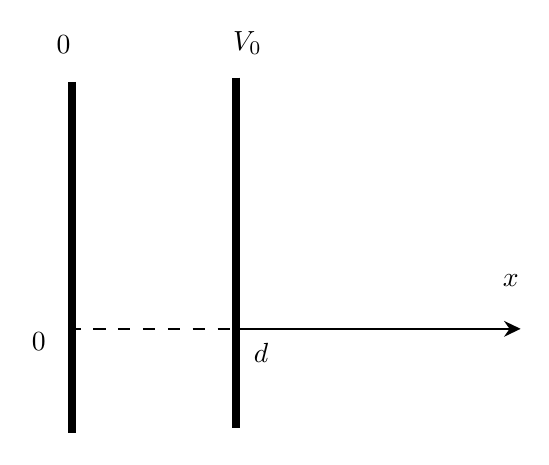
\begin{tikzpicture}[x=0.75pt,y=0.75pt,yscale=-1,xscale=1]
%uncomment if require: \path (0,405); %set diagram left start at 0, and has height of 405

%Straight Lines [id:da57718417654712] 
\draw    (189,211) -- (323,211) ;
\draw [shift={(326,211)}, rotate = 180] [fill={rgb, 255:red, 0; green, 0; blue, 0 }  ][line width=0.08]  [draw opacity=0] (8.04,-3.86) -- (0,0) -- (8.04,3.86) -- (5.34,0) -- cycle    ;
%Straight Lines [id:da33264098994674063] 
\draw [line width=3]    (189,90) -- (189,259) ;
%Straight Lines [id:da5362736509857038] 
\draw [line width=3]    (110,92) -- (110,261) ;
%Straight Lines [id:da5291705370025799] 
\draw  [dash pattern={on 4.5pt off 4.5pt}]  (108,211) -- (189,211) ;

% Text Node
\draw (316,183.4) node [anchor=north west][inner sep=0.75pt]    {$x$};
% Text Node
\draw (196,216.4) node [anchor=north west][inner sep=0.75pt]    {$d$};
% Text Node
\draw (186,66.4) node [anchor=north west][inner sep=0.75pt]    {$V_{0}$};
% Text Node
\draw (101,68.4) node [anchor=north west][inner sep=0.75pt]    {$0$};
% Text Node
\draw (89,211.4) node [anchor=north west][inner sep=0.75pt]    {$0$};


\end{tikzpicture}

\end{center}
\begin{center}
    Hình $1$.
\end{center}
Điện thế thỏa mãn phương trình Poisson:
$$\dfrac{\dd^2 V\tron{x}}{\dd x^2}=-\dfrac{\rho\tron{x}}{\varepsilon_0}=\dfrac{j_0}{\varepsilon_0 v\tron{x}}.$$
Sử dụng hệ thức năng lượng: $\dfrac{1}{2}mv^2\tron{x}=eV$, ta nhận được
$$\dfrac{\dd^2 V\tron{x}}{\dd x^2}=\dfrac{j_0}{\varepsilon_0}\sqrt{\dfrac{m}{2eV\tron{x}}}.$$
Để giải phương trình vi phân này, ta đặt $u=\dfrac{\dd V}{\dd x}.$ Khi đó ta có:
$$\dfrac{\dd^2 V\tron{x}}{\dd x^2}=\dfrac{\dd u}{\dd x}=\dfrac{\dd u}{\dd V}\dfrac{\dd V}{\dd x}=u\dfrac{\dd u}{\dd V},$$
Và phương trình trên trở thành:
$$u\dd u=AV^{-\frac{1}{2}}\dd V,$$
trong đó $A=\dfrac{j_0}{\varepsilon_0}\sqrt{\dfrac{m}{2e}}$.
\\Lưu ý rằng $\dfrac{\dd V}{\dd x}=0$ tại $x=0$, khi các electron nằm yên tại đó. Lấy tích phân phương trình trên ta có:
$$\dfrac{1}{2}u^2=2AV^{\frac{1}{2}},$$
hay
$$V^{-\frac{1}{4}}\dd V=2A^{\frac{1}{2}}\dd x.$$
Vì $V=0$ tại $x=0$ và $V=V_0$ tại $x=d$, tích phân phương trình trên, ta được:
$$\dfrac{4}{3} V_{0}^{\frac{3}{4}}=2 A^{\frac{1}{2}} d=2\left(\dfrac{j_{0}}{\varepsilon_{0}} \sqrt{\dfrac{m}{2 e}}\right)^{\frac{1}{2}} d.$$
Cuối cùng, từ phương trình trên, ta nhận được:
$$\ot{j}=-j_0\ot{e_x}=-\dfrac{4\varepsilon_0V_0}{9d^2}\sqrt{\dfrac{2eV_0}{m}}\ot{e_x}.$$
\end{loigiai}


 \begin{vd}[Suy hao điện tích trong một tụ dò]
 Một tụ cầu có bán kính trong $a$ và bán kính ngoài $b$. Vùng không gian giữa $a<r<b$ được lấp đầy bởi một chất điện môi không cách điện hoàn toàn có hằng số điện môi $\varepsilon_r$ và độ dẫn điện $\sigma$. Ở thời điểm $t=0$, điện tích của tụ là $Q_0$.
 
\begin{center}
\tikzset{every picture/.style={line width=0.75pt}} %set default line width to 0.75pt        

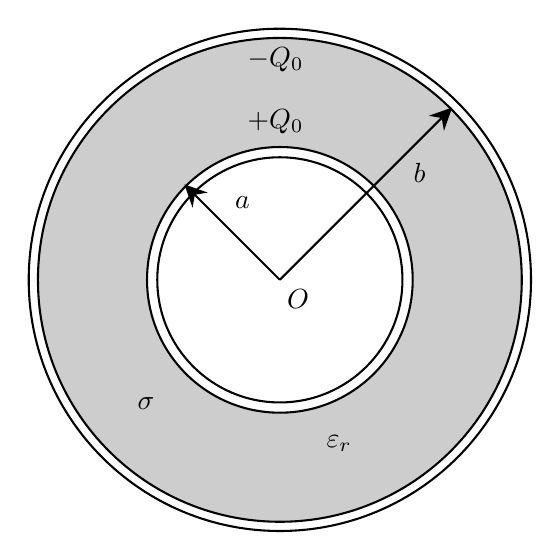
\begin{tikzpicture}[x=0.75pt,y=0.75pt,yscale=-1,xscale=1]
%uncomment if require: \path (0,300); %set diagram left start at 0, and has height of 300

%Flowchart: Connector [id:dp8689538518227609] 
\draw   (144,148) .. controls (144,81.17) and (198.17,27) .. (265,27) .. controls (331.83,27) and (386,81.17) .. (386,148) .. controls (386,214.83) and (331.83,269) .. (265,269) .. controls (198.17,269) and (144,214.83) .. (144,148) -- cycle ;
%Flowchart: Connector [id:dp3998481510353209] 
\draw  [fill={rgb, 255:red, 155; green, 155; blue, 155 }  ,fill opacity=0.5 ] (148.45,148) .. controls (148.45,83.63) and (200.63,31.45) .. (265,31.45) .. controls (329.37,31.45) and (381.55,83.63) .. (381.55,148) .. controls (381.55,212.37) and (329.37,264.55) .. (265,264.55) .. controls (200.63,264.55) and (148.45,212.37) .. (148.45,148) -- cycle ;
%Flowchart: Connector [id:dp5100465094392685] 
\draw  [fill={rgb, 255:red, 255; green, 255; blue, 255 }  ,fill opacity=1 ] (201,148) .. controls (201,112.65) and (229.65,84) .. (265,84) .. controls (300.35,84) and (329,112.65) .. (329,148) .. controls (329,183.35) and (300.35,212) .. (265,212) .. controls (229.65,212) and (201,183.35) .. (201,148) -- cycle ;
%Flowchart: Connector [id:dp8311056122424716] 
\draw   (205.94,148) .. controls (205.94,115.38) and (232.38,88.94) .. (265,88.94) .. controls (297.62,88.94) and (324.06,115.38) .. (324.06,148) .. controls (324.06,180.62) and (297.62,207.06) .. (265,207.06) .. controls (232.38,207.06) and (205.94,180.62) .. (205.94,148) -- cycle ;
%Straight Lines [id:da5001759335183538] 
\draw    (265,148) -- (221.12,104.12) ;
\draw [shift={(219,102)}, rotate = 405] [fill={rgb, 255:red, 0; green, 0; blue, 0 }  ][line width=0.08]  [draw opacity=0] (10.72,-5.15) -- (0,0) -- (10.72,5.15) -- (7.12,0) -- cycle    ;
%Straight Lines [id:da9263270767028116] 
\draw    (265,148) -- (345.88,67.12) ;
\draw [shift={(348,65)}, rotate = 495] [fill={rgb, 255:red, 0; green, 0; blue, 0 }  ][line width=0.08]  [draw opacity=0] (10.72,-5.15) -- (0,0) -- (10.72,5.15) -- (7.12,0) -- cycle    ;


% Text Node
\draw (242,106.4) node [anchor=north west][inner sep=0.75pt]    {$a$};
% Text Node
\draw (328,90.4) node [anchor=north west][inner sep=0.75pt]    {$b$};
% Text Node
\draw (195,203.4) node [anchor=north west][inner sep=0.75pt]    {$\sigma $};
% Text Node
\draw (267,151.4) node [anchor=north west][inner sep=0.75pt]    {$O$};
% Text Node
\draw (286,221.4) node [anchor=north west][inner sep=0.75pt]    {$\varepsilon _{r}$};
% Text Node
\draw (248,34.4) node [anchor=north west][inner sep=0.75pt]    {$-Q_{0}$};
% Text Node
\draw (248,64.4) node [anchor=north west][inner sep=0.75pt]    {$+Q_{0}$};


\end{tikzpicture}
\end{center}
  \begin{enumerate}[1)]
  \item Tìm thời gian đặc trưng của quá trình dò điện trên tụ.
 \item Tìm công suất tỏa nhiệt Joule bên trong tụ và so sánh nó với năng lượng tĩnh điện tức thời.
 \end{enumerate}
\end{vd}
\begin{loigiai}\[\]
  \begin{enumerate}[1)]
  \item Chúng ta dùng hệ tọa độ cầu $(r,\theta,\phi)$, với gốc tọa độ $O$ nằm tại tâm của tụ điện. Chúng ta có $\ot{E} = 0$ tại $r<a$ và $r>b$. Vì hệ có tính đối xứng nên điện trường $\ot{E}$ là theo phương bán kính trong vùng không gian $a<r<b$ và chỉ phụ thuộc vào $r$ và $t$. Điện thông $\varepsilon_r \ot{E} $ thông qua mặt cầu tâm $O$ bán kính $r$ là đồng nhất và không phụ thuộc vào $r$.
   \[\varepsilon_r \oint \ot{E} (r,t) \cdot \dd \ot{S}= 4\pi k_e Q(t) , \tag{1}\]

ở đây $Q(t)$ là điện tích tự do trên bề mặt của quả cầu dẫn điện bán kính $a$. Do đó ta có:
    \[\ot{E}(r,t)= \frac{k_e}{\varepsilon_r} \frac{Q(t)}{r^2}r_c . \tag{2} \]

Ngoài điện tích tự do, hệ còn bao gồm điện tích phân cực tại $r=b$ và $r=a$, có độ lớn lần lượt là $\pm Q(\varepsilon_r -1)/\varepsilon_r$. Không có mật độ điện tích khối bởi vì:
    \[\nabla \cdot \ot{P} = \frac{\varepsilon_r -1}{4\pi k_e} \nabla \cdot \ot{E} (r,t) =0 . \tag{3} \]
Điện trường $\ot{E}(r,t)$ trong vật liệu có độ dẫn điện $\sigma$ sẽ gây ra một mật độ dòng điện $\ot{J}$
      \[\ot{J} = \sigma \ot{E} = \sigma \frac{k_e}{\varepsilon_r}\frac{Q(t)}{r^2} \hat{{r}}, \tag{4} \]

và chúng ta có tổng cường độ dòng điện chạy qua bề mặt:
  \[ I = \frac{\dd Q}{\dd t} = \oint \ot{J} \cdot \dd \ot{S} = \frac{4\pi \sigma k_e}{\varepsilon_r} Q(t). \tag{5}\]

Điện tích bị dịch chuyển đi do điện trường sẽ làm giảm lượng điện tích tự do trên bề mặt quả cầu bên trong, do đó:
  \[\frac{\dd Q(t)}{\dd t}= -\frac{4\pi \sigma k_e}{\varepsilon_r}Q(t), \tag{6}\]

dẫn tới
    \[ Q(t) = Q_0 e^{-t/\tau},\quad \text{với} \quad \tau = \frac{\varepsilon_r}{4\pi\sigma k_e} , \tag{7}\]

và hằng số suy giảm là không phụ thuộc vào kích thước của tụ!
  \item Tổng công suất tỏa nhiệt trên toàn bộ không gian của tụ là:
   \[\begin{aligned} P_d &= \int \ot{J} \cdot \ot{E} \dd^3 x = \sigma \int \ot{E}^2 \dd^3 x = \sigma \int_{a}^{b} \left[ \frac{k_e}{\varepsilon_r} \frac{Q(t)}{r^2}\right] ^2 4 \pi r^2 \dd r \\
    &= \frac{4\pi \sigma k_e^2}{\varepsilon_r^2} Q_0^2 e^{-2t/\tau} \int_{a}^{b} \frac{\dd r}{r^2} = \frac{4\pi \sigma k_e^2 (b-a)}{\varepsilon_r^2 ab} Q_0^2 e^{-2t/\tau} . \end{aligned} \tag{8}\]

Tổng năng lượng tĩnh điện của tụ là:
   \[U_{es} = \frac{1}{2} \frac{Q^2(t)}{C} = \frac{k_e (b-a)}{2 \varepsilon_r ab}Q_0^2 e^{-2t/\tau} , \tag{9}\]

do đó:
  \[\frac{\dd U_{es}}{\dd t} = - \frac{k_e (b-a)}{\tau \varepsilon_r ab} Q_0^2 e^{-2t/\tau} = -\frac{4\pi\sigma k_e^2(b-a)}{\varepsilon_r^2 ab} Q_0^2 e^{-2t/\tau} = -P_d. \tag{10} \]

Vậy, năng lượng tĩnh điện của hệ chỉ mất mát do tỏa nhiệt.
\end{enumerate}
\end{loigiai}



\newpage
\begin{vd}[Tụ phóng và dòng cực đại]%Prob 1C IPhO 2014
\immini{Cho mạch điện như trên hình. Ở thời điểm ban đầu, khoá $S$ ở trạng thái mở và tụ điện có điện dung $2 C$ được tích điện $q_{0}$, tụ điện có điện dung $C$ không tích điện, và không có dòng điện chạy trong các cuộn cảm có độ tự cảm $L$ và $2 L$. Tụ điện bắt đầu phóng điện, và ở đúng thời điểm mà dòng điện trong các cuộn cảm đạt giá trị cực đại thì khóa $S$ được đóng. Tìm giá trị cực đại $I_{\max}$ của dòng điện chạy qua khóa $S$ sau đó.}
{
\tikzset{every picture/.style={line width=0.75pt}} %set default line width to 0.75pt        

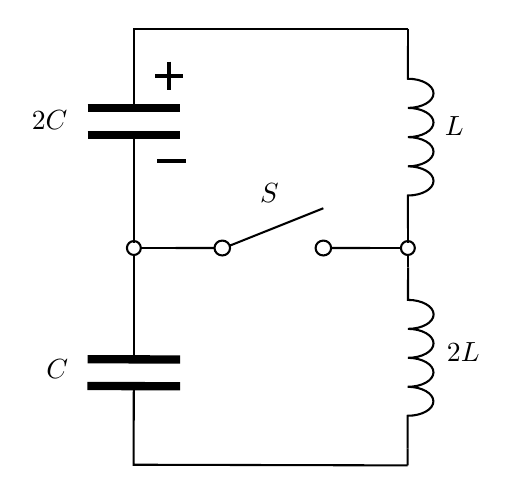
\begin{tikzpicture}[x=0.75pt,y=0.75pt,yscale=-1,xscale=1]
%uncomment if require: \path (0,507); %set diagram left start at 0, and has height of 507

%Straight Lines [id:da26344706665355866] 
\draw [line width=3]    (220.33,141.33) -- (265,141.33) ;
%Shape: Right Angle [id:dp8454753002156017] 
\draw   (242.67,141.33) -- (242.67,103.17) -- (374.67,103.17) ;
%Straight Lines [id:da7011250264858349] 
\draw [line width=3]    (220.33,154.33) -- (265,154.33) ;
%Straight Lines [id:da149592226753412] 
\draw    (242.67,154.33) -- (242.67,206.48) ;
\draw [shift={(242.67,208.83)}, rotate = 90] [color={rgb, 255:red, 0; green, 0; blue, 0 }  ][line width=0.75]      (0, 0) circle [x radius= 3.35, y radius= 3.35]   ;
%Shape: Inductor (Air Core) [id:dp8799427679172205] 
\draw   (374.67,111.44) -- (374.67,127.27) .. controls (381.49,127.27) and (387.03,130.42) .. (387.03,134.3) .. controls (387.03,138.18) and (381.49,141.33) .. (374.67,141.33) .. controls (381.49,141.33) and (387.03,144.48) .. (387.03,148.37) .. controls (387.03,152.25) and (381.49,155.4) .. (374.67,155.4) .. controls (381.49,155.4) and (387.03,158.55) .. (387.03,162.43) .. controls (387.03,166.32) and (381.49,169.47) .. (374.67,169.47) .. controls (381.49,169.47) and (387.03,172.62) .. (387.03,176.5) .. controls (387.03,180.38) and (381.49,183.53) .. (374.67,183.53) -- (374.67,199.36) ;
%Straight Lines [id:da5082876616231975] 
\draw    (374.67,197.11) -- (374.67,206.48) ;
\draw [shift={(374.67,208.83)}, rotate = 90] [color={rgb, 255:red, 0; green, 0; blue, 0 }  ][line width=0.75]      (0, 0) circle [x radius= 3.35, y radius= 3.35]   ;
%Straight Lines [id:da9450311547636574] 
\draw    (374.67,103.17) -- (374.67,111.44) ;
%Shape: Simple Switch [id:dp4720260811074597] 
\draw   (262.78,208.83) -- (281.51,208.83) (337.7,208.83) -- (356.43,208.83) (289,207.64) -- (333.95,189.68) (330.21,208.83) .. controls (330.21,206.85) and (331.88,205.24) .. (333.95,205.24) .. controls (336.02,205.24) and (337.7,206.85) .. (337.7,208.83) .. controls (337.7,210.82) and (336.02,212.42) .. (333.95,212.42) .. controls (331.88,212.42) and (330.21,210.82) .. (330.21,208.83) -- cycle (281.51,208.83) .. controls (281.51,206.85) and (283.19,205.24) .. (285.25,205.24) .. controls (287.32,205.24) and (289,206.85) .. (289,208.83) .. controls (289,210.82) and (287.32,212.42) .. (285.25,212.42) .. controls (283.19,212.42) and (281.51,210.82) .. (281.51,208.83) -- cycle ;
%Straight Lines [id:da906656742067266] 
\draw    (246.33,208.83) -- (262.78,208.83) ;
%Straight Lines [id:da5775940818375183] 
\draw    (356.43,208.83) -- (371.29,208.83) ;
%Straight Lines [id:da4066291176338004] 
\draw [line width=3]    (220.29,275.32) -- (264.96,275.42) ;
%Shape: Right Angle [id:dp183719375392559] 
\draw   (242.63,275.37) -- (242.53,313.24) -- (374.53,313.56) ;
%Straight Lines [id:da4194311109878792] 
\draw [line width=3]    (220.33,262.42) -- (264.99,262.53) ;
%Shape: Inductor (Air Core) [id:dp3140477071504184] 
\draw   (374.55,305.35) -- (374.59,289.65) .. controls (381.42,289.66) and (386.96,286.55) .. (386.97,282.7) .. controls (386.98,278.85) and (381.45,275.71) .. (374.63,275.69) .. controls (381.45,275.71) and (387,272.59) .. (387.01,268.74) .. controls (387.02,264.89) and (381.48,261.75) .. (374.66,261.73) .. controls (381.48,261.75) and (387.03,258.64) .. (387.04,254.79) .. controls (387.05,250.94) and (381.52,247.8) .. (374.69,247.78) .. controls (381.52,247.8) and (387.07,244.68) .. (387.08,240.83) .. controls (387.09,236.98) and (381.55,233.84) .. (374.73,233.82) -- (374.77,218.12) ;
%Straight Lines [id:da6089515590426191] 
\draw    (374.53,313.56) -- (374.55,305.35) ;
%Straight Lines [id:da2296661541164089] 
\draw    (242.66,212.53) -- (242.66,262.47) ;
%Straight Lines [id:da06067953052238306] 
\draw    (374.77,212.39) -- (374.77,218.12) ;
\draw  [line width=1.5]  (253,125.75) -- (266.5,125.75)(259.75,119) -- (259.75,132.5) ;
%Straight Lines [id:da794615618747962] 
\draw [line width=1.5]    (254,167) -- (267.67,167) ;

% Text Node
\draw (192,141.07) node [anchor=north west][inner sep=0.75pt]    {$2C$};
% Text Node
\draw (199,261.07) node [anchor=north west][inner sep=0.75pt]    {$C$};
% Text Node
\draw (302,176.07) node [anchor=north west][inner sep=0.75pt]    {$S$};
% Text Node
\draw (391,144.07) node [anchor=north west][inner sep=0.75pt]    {$L$};
% Text Node
\draw (392,253.07) node [anchor=north west][inner sep=0.75pt]    {$2L$};
\end{tikzpicture}
}
\end{vd}
\begin{loigiai}\\
\textit{Bài toán này có thể được giải bằng nhiều cách khác nhau. Dưới đây là một số cách giải.}\\
\textbf{Cách 1.}Phương pháp tiếp cận trực tiếp.\\
    Tại thời điểm cường độ dòng điện trong các cuộn dây đạt cực đại, tổng hiệu điện thế giữa hai đầu các cuộn dây bằng $0$, vì vậy điện áp của hai tụ điện phải bằng nhau về độ lớn và trái dấu. Gọi $U$ là điện áp trên của các tụ điện tại thời điểm dòng điện đạt giá trị cực đại $I_0$. Theo định luật bảo toàn điện tích.
    \[q_0 = 2CU + CU \tag{1.1} \label{q.11.1.1} \]
    \[\rt U=\dfrac{q_{0}}{3 C}. \tag{1.2} \label{q.11.1.2} \]
    Khi đó, theo định luật bảo toàn năng lượng:
    \[\dfrac{q_{0}^{2}}{2 \cdot 2 C}=\dfrac{L I_{0}^{2}}{2}+\dfrac{2 L I_{0}^{2}}{2}+\dfrac{C U^{2}}{2}+\dfrac{2 C U^{2}}{2}.\tag{1.3} \label{q.11.1.3}\]
    Dòng điện cực đại:
    \[I_{0}=\dfrac{q_{0}}{3 \sqrt{2 L C}}. \tag{1.4} \label{q.11.1.4}\]
    Sau khi khóa được đóng sẽ có dao động độc lập trong cả hai mạch với tần số:
    \[\omega = \dfrac{1}{\sqrt{2 L C}}. \tag{1.5} \label{q.11.1.5}\]
    Và biên độ của chúng được suy ra từ định luật bảo toàn năng lượng tưong ứng với các mạch được viết như sau:
    \[\dfrac{2 C U^{2}}{2}+\dfrac{L I_{0}^{2}}{2} = \dfrac{4 J_{1}^{2}}{2}, \tag{1.6} \label{q.11.1.6}\]
    \[\dfrac{C U^{2}}{2}+\dfrac{2 L I_{0}^{2}}{2} = \dfrac{2 LJ_2^{2}}{2}.\tag{1.7} \label{q.11.1.7}\]
    \immini{
    Do đó, biên độ tương ứng là:
    \[J_1 = \sqrt{5} I_0, \tag{1.8} \label{q.11.1.8}\]
    \[J_2 = \sqrt{2}I_0.\tag{1.9} \label{q.11.1.9}\]
    Chọn chiều dương của các dòng điện trong mạch như hình vẽ. Khi đó, dòng điện chạy qua khoá $S$ được viết như sau:
    \[I = I_1 - I_2. \tag{1.10} \label{q.11.1.10}\]}
    {

\tikzset{every picture/.style={line width=0.75pt}} %set default line width to 0.75pt        

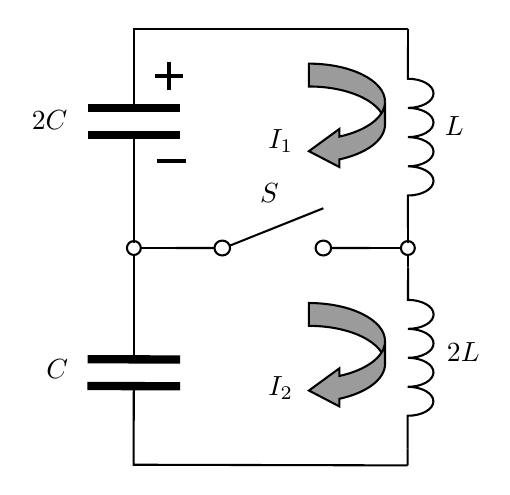
\begin{tikzpicture}[x=0.75pt,y=0.75pt,yscale=-1,xscale=1]
%uncomment if require: \path (0,507); %set diagram left start at 0, and has height of 507

%Straight Lines [id:da26344706665355866] 
\draw [line width=3]    (220.33,141.33) -- (265,141.33) ;
%Shape: Right Angle [id:dp8454753002156017] 
\draw   (242.67,141.33) -- (242.67,103.17) -- (374.67,103.17) ;
%Straight Lines [id:da7011250264858349] 
\draw [line width=3]    (220.33,154.33) -- (265,154.33) ;
%Straight Lines [id:da149592226753412] 
\draw    (242.67,154.33) -- (242.67,206.48) ;
\draw [shift={(242.67,208.83)}, rotate = 90] [color={rgb, 255:red, 0; green, 0; blue, 0 }  ][line width=0.75]      (0, 0) circle [x radius= 3.35, y radius= 3.35]   ;
%Shape: Inductor (Air Core) [id:dp8799427679172205] 
\draw   (374.67,111.44) -- (374.67,127.27) .. controls (381.49,127.27) and (387.03,130.42) .. (387.03,134.3) .. controls (387.03,138.18) and (381.49,141.33) .. (374.67,141.33) .. controls (381.49,141.33) and (387.03,144.48) .. (387.03,148.37) .. controls (387.03,152.25) and (381.49,155.4) .. (374.67,155.4) .. controls (381.49,155.4) and (387.03,158.55) .. (387.03,162.43) .. controls (387.03,166.32) and (381.49,169.47) .. (374.67,169.47) .. controls (381.49,169.47) and (387.03,172.62) .. (387.03,176.5) .. controls (387.03,180.38) and (381.49,183.53) .. (374.67,183.53) -- (374.67,199.36) ;
%Straight Lines [id:da5082876616231975] 
\draw    (374.67,197.11) -- (374.67,206.48) ;
\draw [shift={(374.67,208.83)}, rotate = 90] [color={rgb, 255:red, 0; green, 0; blue, 0 }  ][line width=0.75]      (0, 0) circle [x radius= 3.35, y radius= 3.35]   ;
%Straight Lines [id:da9450311547636574] 
\draw    (374.67,103.17) -- (374.67,111.44) ;
%Shape: Simple Switch [id:dp4720260811074597] 
\draw   (262.78,208.83) -- (281.51,208.83) (337.7,208.83) -- (356.43,208.83) (289,207.64) -- (333.95,189.68) (330.21,208.83) .. controls (330.21,206.85) and (331.88,205.24) .. (333.95,205.24) .. controls (336.02,205.24) and (337.7,206.85) .. (337.7,208.83) .. controls (337.7,210.82) and (336.02,212.42) .. (333.95,212.42) .. controls (331.88,212.42) and (330.21,210.82) .. (330.21,208.83) -- cycle (281.51,208.83) .. controls (281.51,206.85) and (283.19,205.24) .. (285.25,205.24) .. controls (287.32,205.24) and (289,206.85) .. (289,208.83) .. controls (289,210.82) and (287.32,212.42) .. (285.25,212.42) .. controls (283.19,212.42) and (281.51,210.82) .. (281.51,208.83) -- cycle ;
%Straight Lines [id:da906656742067266] 
\draw    (246.33,208.83) -- (262.78,208.83) ;
%Straight Lines [id:da5775940818375183] 
\draw    (356.43,208.83) -- (371.29,208.83) ;
%Straight Lines [id:da4066291176338004] 
\draw [line width=3]    (220.29,275.32) -- (264.96,275.42) ;
%Shape: Right Angle [id:dp183719375392559] 
\draw   (242.63,275.37) -- (242.53,313.24) -- (374.53,313.56) ;
%Straight Lines [id:da4194311109878792] 
\draw [line width=3]    (220.33,262.42) -- (264.99,262.53) ;
%Shape: Inductor (Air Core) [id:dp3140477071504184] 
\draw   (374.55,305.35) -- (374.59,289.65) .. controls (381.42,289.66) and (386.96,286.55) .. (386.97,282.7) .. controls (386.98,278.85) and (381.45,275.71) .. (374.63,275.69) .. controls (381.45,275.71) and (387,272.59) .. (387.01,268.74) .. controls (387.02,264.89) and (381.48,261.75) .. (374.66,261.73) .. controls (381.48,261.75) and (387.03,258.64) .. (387.04,254.79) .. controls (387.05,250.94) and (381.52,247.8) .. (374.69,247.78) .. controls (381.52,247.8) and (387.07,244.68) .. (387.08,240.83) .. controls (387.09,236.98) and (381.55,233.84) .. (374.73,233.82) -- (374.77,218.12) ;
%Straight Lines [id:da6089515590426191] 
\draw    (374.53,313.56) -- (374.55,305.35) ;
%Straight Lines [id:da2296661541164089] 
\draw    (242.66,212.53) -- (242.66,262.47) ;
%Straight Lines [id:da06067953052238306] 
\draw    (374.77,212.39) -- (374.77,218.12) ;
\draw  [line width=1.5]  (253,125.75) -- (266.5,125.75)(259.75,119) -- (259.75,132.5) ;
%Straight Lines [id:da794615618747962] 
\draw [line width=1.5]    (254,167) -- (267.67,167) ;
%Curve Right Arrow [id:dp8522988656363095] 
\draw  [fill={rgb, 255:red, 155; green, 155; blue, 155 }  ,fill opacity=1 ] (363.67,149.33) .. controls (363.67,139.21) and (347.25,131) .. (327,131) -- (327,120) .. controls (347.25,120) and (363.67,128.21) .. (363.67,138.33) ;\draw  [fill={rgb, 255:red, 155; green, 155; blue, 155 }  ,fill opacity=1 ] (363.67,138.33) .. controls (363.67,145.85) and (354.62,152.31) .. (341.67,155.14) -- (341.67,151.47) -- (327,162.17) -- (341.67,169.81) -- (341.67,166.14) .. controls (354.62,163.31) and (363.67,156.85) .. (363.67,149.33)(363.67,138.33) -- (363.67,149.33) ;
%Curve Right Arrow [id:dp7288764250559718] 
\draw  [fill={rgb, 255:red, 155; green, 155; blue, 155 }  ,fill opacity=1 ] (363.67,264.67) .. controls (363.67,254.54) and (347.25,246.33) .. (327,246.33) -- (327,235.33) .. controls (347.25,235.33) and (363.67,243.54) .. (363.67,253.67) ;\draw  [fill={rgb, 255:red, 155; green, 155; blue, 155 }  ,fill opacity=1 ] (363.67,253.67) .. controls (363.67,261.18) and (354.62,267.65) .. (341.67,270.47) -- (341.67,266.81) -- (327,277.5) -- (341.67,285.14) -- (341.67,281.47) .. controls (354.62,278.65) and (363.67,272.18) .. (363.67,264.67)(363.67,253.67) -- (363.67,264.67) ;

% Text Node
\draw (192,141.07) node [anchor=north west][inner sep=0.75pt]    {$2C$};
% Text Node
\draw (199,261.07) node [anchor=north west][inner sep=0.75pt]    {$C$};
% Text Node
\draw (302,176.07) node [anchor=north west][inner sep=0.75pt]    {$S$};
% Text Node
\draw (391,144.07) node [anchor=north west][inner sep=0.75pt]    {$L$};
% Text Node
\draw (392,253.07) node [anchor=north west][inner sep=0.75pt]    {$2L$};
% Text Node
\draw (306,150.4) node [anchor=north west][inner sep=0.75pt]    {$I_{1}$};
% Text Node
\draw (306,269.4) node [anchor=north west][inner sep=0.75pt]    {$I_{2}$};
\end{tikzpicture}
}
    Các dòng điện phụ thuộc vào thời gian như sau:
    \[ I_1(t) = A\cos \omega t + B \sin \omega t, \tag{1.11} \label{q.11.1.11}\]
    \[I_2(t) = D \cos \omega t + F \sin \omega t. \tag{1.12} \label{q.11.1.12}\]
    Các hằng số $A, B, D, F$ có thể được xác định từ các giá trị ban đầu của dòng điện và biên độ của chúng bằng cách thay vào các phương trình sau:
    \[ I_1(0) = A = I_0,\tag{1.13} \label{q.11.1.13}\]
    \[A^2 + B^2 = J_1^2,\tag{1.14} \label{q.11.1.14}\]
    \[I_2(0) = D = I_0,\tag{1.15} \label{q.11.1.15}\]
    \[D^2 + F^2 = J_2^2.\tag{1.16} \label{q.11.1.16}\]
    Giải hệ phương trình (\ref{q.11.1.13}) - (\ref{q.11.1.16}), ta được
    \[B = 2I_0,\tag{1.17} \label{q.11.1.17}\]
    \[F = -I_0,\tag{1.18} \label{q.11.1.18}\]
    Dấu của $F$ được chọn là âm vì tại thời điểm khoá $S$ đóng, dòng điện trong cuộn cảm $2L$ đang giảm.\\
    Do đó, sự phụ thuộc của các dòng điện vào thời gian $t$ là:
    \[I_1(t) = I_0 \tron{\cos \omega t + 2\sin \omega t}, \tag{1.19} \label{q.11.1.19}\]
    \[I_2(t) = I_0 \tron{\cos \omega t - \sin \omega t},\tag{1.20} \label{q.11.1.20}\]
    Theo phương trình (\ref{q.11.1.10}), dòng điện qua khoá $S$ phụ thuộc vào thời gian theo biểu thức:
    \[I(t) = I_1(t) - I_2(t) = 3I_0 \sin \omega t. \tag{1.21} \label{q.11.1.21} \]
    Do đó, biện độ của dòng điện qua khoá $S$ được tính bởi:
    \[I_{\max} = 3I_0 = \omega q_0 = \dfrac{q_0}{\sqrt{2LC}}. \tag{1.22} \label{q.11.1.22}\]
    
    \textbf{Cách 2.} Dùng giản đồ Vector\\
    Thay vì xác định các hệ số $A, B, D, F$, ta vẽ giản đồ vector như hình vẽ sau.
    \begin{center}
\tikzset{every picture/.style={line width=0.75pt}} %set default line width to 0.75pt        

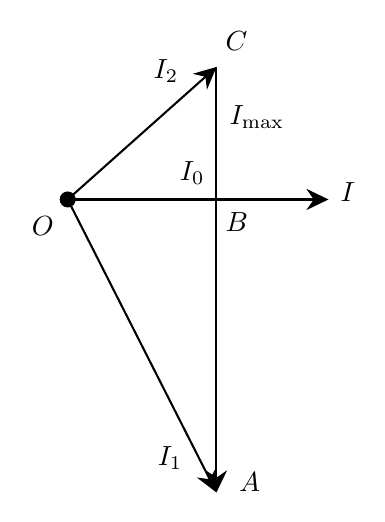
\begin{tikzpicture}[x=0.75pt,y=0.75pt,yscale=-1,xscale=1]
%uncomment if require: \path (0,470); %set diagram left start at 0, and has height of 470

%Straight Lines [id:da7202886787716356] 
\draw    (221,151) -- (343.67,151) ;
\draw [shift={(346.67,151)}, rotate = 180] [fill={rgb, 255:red, 0; green, 0; blue, 0 }  ][line width=0.08]  [draw opacity=0] (10.72,-5.15) -- (0,0) -- (10.72,5.15) -- (7.12,0) -- cycle    ;
\draw [shift={(221,151)}, rotate = 0] [color={rgb, 255:red, 0; green, 0; blue, 0 }  ][fill={rgb, 255:red, 0; green, 0; blue, 0 }  ][line width=0.75]      (0, 0) circle [x radius= 3.35, y radius= 3.35]   ;
%Straight Lines [id:da3460435475707393] 
\draw    (221,151) -- (290.43,89.16) ;
\draw [shift={(292.67,87.17)}, rotate = 498.31] [fill={rgb, 255:red, 0; green, 0; blue, 0 }  ][line width=0.08]  [draw opacity=0] (10.72,-5.15) -- (0,0) -- (10.72,5.15) -- (7.12,0) -- cycle    ;
%Straight Lines [id:da2677047873071534] 
\draw    (221,151) -- (291.31,289.49) ;
\draw [shift={(292.67,292.17)}, rotate = 243.07999999999998] [fill={rgb, 255:red, 0; green, 0; blue, 0 }  ][line width=0.08]  [draw opacity=0] (10.72,-5.15) -- (0,0) -- (10.72,5.15) -- (7.12,0) -- cycle    ;
%Straight Lines [id:da6430056460999514] 
\draw    (292.67,87.17) -- (292.67,289.17) ;
\draw [shift={(292.67,292.17)}, rotate = 270] [fill={rgb, 255:red, 0; green, 0; blue, 0 }  ][line width=0.08]  [draw opacity=0] (10.72,-5.15) -- (0,0) -- (10.72,5.15) -- (7.12,0) -- cycle    ;

% Text Node
\draw (351,141.4) node [anchor=north west][inner sep=0.75pt]    {$I$};
% Text Node
\draw (260.89,82.07) node [anchor=north west][inner sep=0.75pt]    {$I_{2}$};
% Text Node
\draw (262.89,268.73) node [anchor=north west][inner sep=0.75pt]    {$I_{1}$};
% Text Node
\draw (202.22,157.84) node [anchor=north west][inner sep=0.75pt]    {$O$};
% Text Node
\draw (302.22,281.18) node [anchor=north west][inner sep=0.75pt]    {$A$};
% Text Node
\draw (295.56,155.84) node [anchor=north west][inner sep=0.75pt]    {$B$};
% Text Node
\draw (295.56,68.73) node [anchor=north west][inner sep=0.75pt]    {$C$};
% Text Node
\draw (273.56,131.07) node [anchor=north west][inner sep=0.75pt]    {$I_{0}$};
% Text Node
\draw (297.56,104.18) node [anchor=north west][inner sep=0.75pt]    {$I_{\max}$};
\end{tikzpicture}
    \end{center}
    Đoạn $AC$ biểu thị dòng điện và hình chiếu của nó trên trục dòng điện là bằng $0$ tại thời điểm đóng khóa $S$. Dòng điện $I_{1}$ trong cuộn cảm $L$ tăng tại thời điểm đó vì tụ điện $2 C$ tiếp tục phóng điện, do đó, dòng điện này được mô tả trong hình bằng đoạn $O A$. Dòng điện $I_{2}$ trong cuộn cảm $2 L$ giảm tại thời điểm đóng khóa $S$ vì nó tiếp tục nạp điện cho tụ điện $2 C$, đó là lý do tại sao dòng điện $I_{2}$ được mô tả trong hình bằng đoạn $O C$.\\
    Ta biết rằng tại đó:
    \[OB = I_{0}, O A=\sqrt{5} I_{0}, OC = \sqrt{2} I_{0}\]
    Do đó, từ định lý Pythagore ta tính được:
    \[A B=\sqrt{O A^{2}-O B^{2}}=2 I_{0} \tag{2.1} \label{q.11.2.1}\]
    \[B C=\sqrt{O C^{2}-O B^{2}}=I_{0}\tag{2.2} \label{q.11.2.2}\]
    Vì vậy, dòng điện cực đại là:
    \[I_{\max} = AC =AB + BC = 3 I_{0} = \omega q_{0}=\dfrac{q_{0}}{\sqrt{2 L C}} \tag{2.3} \label{q.11.2.3}\]
    \textbf{Cách 3.} Cách tiếp cận phỏng đoán.\\
    Rõ ràng là dòng điện qua khóa $S$ thực hiện dao động điều hòa với tần số:
    \[\omega=\dfrac{1}{\sqrt{2 L C}}, \tag{3.1} \label{q.11.3.1}\]
    và nó bằng $0$ tại thời điểm đóng khóa $S$, tức là:
    \[I(t)=I_{\max} \sin \omega t. \tag{3.2} \label{q.11.3.2}\]
    Vì dòng điện bằng $0$ tại thời điểm đóng khóa $S$, biên độ dòng điện bằng với đạo hàm của dòng điện tại thời điểm này chia cho tần số dao động. Chúng ta đi tìm đạo hàm của dòng điện. Gọi $q_{1}$ là điện tích của tụ điện có điện dung $2 C$. Khi đó, điện tích trên tụ điện có điện dung $C$ được tìm thấy từ định luật bảo toàn điện tích
    \[q_{2}=q_{0}-q_{1}.\tag{3.3} \label{q.11.3.3} \]
    Sau khi đóng khóa $S$, tốc độ thay đổi dòng điện trong cuộn cảm $L$ là:
    \[\dot{I}_{1}=\dfrac{q_{1}}{2 L C}.\tag{3.4} \label{q.11.3.4}\]
    Trong khi đó, đối với cuộn dây có độ tự cảm $2 L$ bằng:
    \[\dot{I}_{2}=-\dfrac{q_{0}-q_{1}}{2 L C}. \tag{3.5} \label{q.11.3.5}\]
    Do điện áp đặt lên các tụ điện là ngược dấu, do đó đạo hàm của dòng điện đối với thời gian cuối cùng có dạng:
    \[\dot{I} = \dot{I}_{1} - \dot{I}_{2} = \dfrac{q_{0}}{2 L C} = \omega^{2} q_{0}\tag{3.6} \label{q.11.3.6}\]
    \textbf{Lưu ý.} Đạo hàm này độc lập với thời gian đóng khóa $S$!\\
    Do đó, dòng điện cực đại qua khoá $S$ là:
    \[I_{\max }=\dfrac{\dot{I}}{\omega}=\omega q_{0} = \dfrac{q_{0}}{\sqrt{2 L C}}\tag{3.7} \label{q.11.3.7}\]
    và nó độc lập với thời gian đóng khóa $S$!


\end{loigiai}
\begin{vd}[Mạch kích điện áp một chiều]
Loại xe hybrid điện và xăng hiện đại đòi hỏi điện áp cao để điều khiển động cơ của chúng từ pin có điện thế thấp hơn. Dòng điện xoay chiều (AC) có thể được tăng lên một cách dễ dàng bằng cách sử dụng các máy biến áp, nhưng điện áp dòng điện một chiều (DC) đòi hỏi thiết kế phức tạp hơn. Trong bài toán này, chúng ta nghiên cứu mạch kích điện một chiều có mạch cấu tạo như hình vẽ; gồm một nguồn điện thế vào $V_{i}$, một cuộn thuần cảm có độ tự cảm $L$, tụ điện có điện dung $C$, điện trở $R$ và diode lí tưởng $D$ (khi dòng thuận đi qua thì điện trở của $D$ bằng không và khi dòng ngược thì điện trở của $D$ bằng vô cùng).
\begin{center}
    

\tikzset{every picture/.style={line width=0.75pt}} %set default line width to 0.75pt        

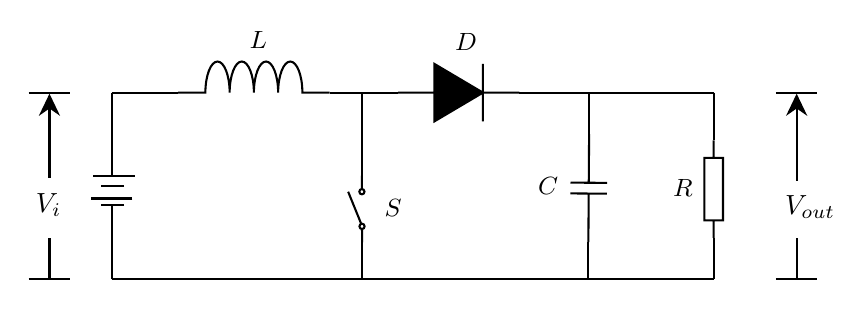
\begin{tikzpicture}[x=0.75pt,y=0.75pt,yscale=-1,xscale=1]
%uncomment if require: \path (0,300); %set diagram left start at 0, and has height of 300

%Shape: Inductor (Air Core) [id:dp7223413828463101] 
\draw   (112,120.2) -- (125.14,120.2) .. controls (125.14,111.92) and (127.76,105.2) .. (130.98,105.2) .. controls (134.21,105.2) and (136.83,111.92) .. (136.83,120.2) .. controls (136.83,111.92) and (139.44,105.2) .. (142.67,105.2) .. controls (145.89,105.2) and (148.51,111.92) .. (148.51,120.2) .. controls (148.51,111.92) and (151.13,105.2) .. (154.35,105.2) .. controls (157.57,105.2) and (160.19,111.92) .. (160.19,120.2) .. controls (160.19,111.92) and (162.81,105.2) .. (166.03,105.2) .. controls (169.26,105.2) and (171.87,111.92) .. (171.87,120.2) -- (185.02,120.2) ;
%Straight Lines [id:da2584191430229441] 
\draw    (185.02,120.2) -- (218.02,120.2) ;
%Shape: Diode [id:dp23920160245954047] 
\draw  [fill={rgb, 255:red, 0; green, 0; blue, 0 }  ,fill opacity=1 ] (235.53,106.39) -- (258.87,120.2) -- (235.53,134.01) -- (235.53,106.39) -- cycle (218.02,120.2) -- (235.53,120.2) (258.87,106.39) -- (258.87,134.01) (258.87,120.2) -- (276.38,120.2) ;
%Straight Lines [id:da9643863182670489] 
\draw    (276.38,120.2) -- (370.02,120.2) ;
%Shape: Resistor [id:dp039146831292158346] 
\draw   (374.52,151.66) -- (374.54,181.74) -- (365.54,181.74) -- (365.52,151.66) -- (374.52,151.66) -- cycle (370.02,143.2) -- (370.02,151.66) (370.04,181.74) -- (370.04,190.2) ;
%Straight Lines [id:da5255761377437085] 
\draw    (370.02,120.2) -- (370.02,143.2) ;
%Straight Lines [id:da27774903104069804] 
\draw    (370.04,190.2) -- (370.04,210.2) ;
%Straight Lines [id:da7136757057576355] 
\draw    (310.02,120.2) -- (310.02,140.2) ;
%Shape: Capacitor [id:dp031376412371586504] 
\draw   (310.02,140.2) -- (309.85,163.61) (318.63,168.88) -- (301.01,168.75) (318.66,163.67) -- (301.05,163.55) (309.82,168.81) -- (309.66,192.23) ;
%Straight Lines [id:da5888494213877151] 
\draw    (309.66,192.23) -- (309.66,210.2) ;
%Straight Lines [id:da029385651055682915] 
\draw    (80.02,210.2) -- (370.04,210.2) ;
%Straight Lines [id:da19558707003497977] 
\draw    (80.02,120.2) -- (112,120.2) ;
%Straight Lines [id:da7718653354203724] 
\draw    (80.02,210.2) -- (80.02,174.2) ;
%Straight Lines [id:da7827525948111083] 
\draw    (90.02,171.2) -- (70.02,171.2) ;
%Straight Lines [id:da5365489525546694] 
\draw    (91.02,160.2) -- (71.02,160.2) ;
%Straight Lines [id:da5598912472205531] 
\draw    (86.02,174.2) -- (75.02,174.2) ;
%Straight Lines [id:da3874602761186867] 
\draw    (86.02,165.2) -- (75.02,165.2) ;
%Straight Lines [id:da5891789301788788] 
\draw    (80.02,160.2) -- (80.02,120.2) ;
%Straight Lines [id:da3878997408989351] 
\draw    (200.52,160.2) -- (200.52,120.2) ;
%Shape: Simple Switch [id:dp04631457380122894] 
\draw   (200.64,192.34) -- (200.61,185.91) (200.54,166.63) -- (200.52,160.2) (200.19,183.34) -- (193.93,167.94) (200.55,169.2) .. controls (199.87,169.2) and (199.31,168.63) .. (199.31,167.92) .. controls (199.3,167.21) and (199.86,166.63) .. (200.54,166.63) .. controls (201.23,166.62) and (201.78,167.2) .. (201.79,167.91) .. controls (201.79,168.62) and (201.24,169.19) .. (200.55,169.2) -- cycle (200.61,185.91) .. controls (199.93,185.91) and (199.37,185.34) .. (199.37,184.63) .. controls (199.37,183.92) and (199.92,183.34) .. (200.6,183.34) .. controls (201.29,183.34) and (201.84,183.91) .. (201.85,184.62) .. controls (201.85,185.33) and (201.3,185.91) .. (200.61,185.91) -- cycle ;
%Straight Lines [id:da8729955824300575] 
\draw    (200.64,209.7) -- (200.64,192.34) ;
%Straight Lines [id:da766550663793581] 
\draw    (400.02,210.2) -- (420.02,210.2) ;
%Straight Lines [id:da0002445122940570865] 
\draw    (400.02,120.2) -- (420.02,120.2) ;
%Straight Lines [id:da6908529248928172] 
\draw    (410.02,123.7) -- (410.02,162.7) ;
\draw [shift={(410.02,120.7)}, rotate = 90] [fill={rgb, 255:red, 0; green, 0; blue, 0 }  ][line width=0.08]  [draw opacity=0] (10.72,-5.15) -- (0,0) -- (10.72,5.15) -- (7.12,0) -- cycle    ;
%Straight Lines [id:da481976252749885] 
\draw    (40.02,210.2) -- (60.02,210.2) ;
%Straight Lines [id:da01284165805310189] 
\draw    (40.02,120.2) -- (60.02,120.2) ;
%Straight Lines [id:da08238213380831083] 
\draw    (50.02,123.7) -- (50.02,161.2) ;
\draw [shift={(50.02,120.7)}, rotate = 90] [fill={rgb, 255:red, 0; green, 0; blue, 0 }  ][line width=0.08]  [draw opacity=0] (10.72,-5.15) -- (0,0) -- (10.72,5.15) -- (7.12,0) -- cycle    ;
%Straight Lines [id:da6240970111466693] 
\draw    (410.02,210.2) -- (410.02,190.2) ;
%Straight Lines [id:da10220899399995531] 
\draw    (50.02,210.2) -- (50.02,190.2) ;

% Text Node
\draw (349,160.4) node [anchor=north west][inner sep=0.75pt]  [font=\small]  {$R$};
% Text Node
\draw (244,90.4) node [anchor=north west][inner sep=0.75pt]  [font=\small]  {$D$};
% Text Node
\draw (145,89.4) node [anchor=north west][inner sep=0.75pt]  [font=\small]  {$L$};
% Text Node
\draw (284,159.4) node [anchor=north west][inner sep=0.75pt]  [font=\small]  {$C$};
% Text Node
\draw (42,167.4) node [anchor=north west][inner sep=0.75pt]    {$V_{i}$};
% Text Node
\draw (403,168.4) node [anchor=north west][inner sep=0.75pt]    {$V_{\text{out}}$};
% Text Node
\draw (210,170.4) node [anchor=north west][inner sep=0.75pt]  [font=\small]  {$S$};


\end{tikzpicture}
\end{center}
Khóa $S$ được điều khiển bởi một mạch điện khác không được thể hiện trong hình vẽ. Khóa đóng mở tuần hoàn với tần số cao. Một chu kì bao gồm một trạng thái đóng và một trạng thái mở. Trạng thái đóng kéo dài trong thời gian $t_1$ và trạng thái mở kéo dài trong thời gian $t_0$.
\begin{enumerate}[1) ]
    \item Tại thời điểm ban đầu, dòng điện trong mạch bằng $0$ và tụ điện không tích điện. Tại thời điểm $t=0$ khóa $S$ đóng. Tính cường độ dòng điện qua cuộn cảm tại thời điểm $t=t_1$.
    \item Tại thời điểm $t=t_1$, khóa $S$ mở. Tính dòng điện qua cuộn cảm tại thời điểm $t$ trong chu kì khóa mở $(t_1<t<t_1+t_0)$. Giả thiết rằng điện trở $R$ đủ lớn để có thể bỏ qua dòng điện chạy qua nó.\\
\end{enumerate}
 Trong các phần tiếp theo, ta xét chế độ hoạt động sao cho $t_1+t_0\ll\sqrt{LC}$. Trong chế độ này, khi tính toán ta chỉ cần giữ lại các đại lượng tỉ lệ thuận với $t_1$ và $t_0$.
\\
\begin{enumerate}  [1)]  
   \setcounter{enumi}{2}
    \item Tìm mối quan hệ giữa dòng đi qua cuộn cảm ở cuối chu kì mở thứ $n-1$  và cuối chu kì đóng thứ $n$, kí hiệu là $I_0(n-1)$ và $I_1(n)$.
    \item Ở chu kì đóng thứ $n$, dòng qua tải đủ lớn để phải tính đến giá trị của nó. Tìm liên hệ giữa điện áp trên tụ điện ở cuối chu kì mở thứ $n-1$ và cuối chu kì đóng thứ $n$, kí hiệu là $V_0(n-1)$ và $V_1(n)$.
    \item Ở cuối chu kì đóng thứ $n$, dòng điện qua cuộn cảm là $I_1(n)$ và điện áp trên tụ là $V_1(n)$. Tính dòng qua cuộn cảm $I_0(n)$ và điện áp trên tụ $V_0(n)$ ở cuối chu kì mở ngay sau đó.
    \item Khi hệ đạt đến trạng thái ổn định, tính tỉ số kích điện áp $\dfrac{V_{\text{out}}}{V_{i}}$. Để tăng tỉ số này lên, ta phải chọn $t_1$ và $t_0$ như thế nào?
    \item Tính dòng điện qua cuộn cảm trong chu kỳ đóng đạt trạng thái ổn định. Giải thích ý nghĩa vật lí của kết quả.
    \item Giải thích tầm quan trọng của diode trong mạch kích điện áp một chiều này.
    \item Ước tính thời gian cần thiết để đạt đến trạng thái ổn định. Chỉ sử dụng các đại lượng $t_1$, $t_0$, $L$, $C$, $R$ để diễn tả kết quả của bạn.
\end{enumerate}
\end{vd}
\begin{loigiai}\[\]
\begin{enumerate}[1) ]
    \item Khi khóa $S$ đóng, diode, tụ điện và điện trở có thể bỏ qua. Do đó
    \begin{align*}
        &V_{i}-L\dfrac{\mathrm{d}I}{\mathrm{d}t}=0\\
        &\rt I=\int_{0}^{t_1}\dfrac{V_{i}}{L}\mathrm{d}t=\dfrac{V_{i}}{L}t_1.
    \end{align*}
    \item Khi khóa $S$ mở, mạch điện bao gồm nguồn điện, cuộn cảm, diode và tụ điện (bỏ qua điện trở). \\
    Theo giả thiết điện trở của diode bằng $0$.
    \begin{align*}
        &V_{i}-L\dfrac{\mathrm{d}I}{\mathrm{d}t}-\dfrac{q}{LC}=0\\
        &I=\dfrac{\mathrm{d}q}{\mathrm{d}t}\\
        &\dfrac{\mathrm{d}^2q}{\mathrm{d}t^2}+\dfrac{q}{LC}=\dfrac{V_{i}}{L}\rt \dfrac{\mathrm{d}^2q}{\mathrm{d}t^2}+\dfrac{1}{LC}(q-CV_{i})=0
    \end{align*}
    Đại lượng $q-CV_{i}$ là một dao động điều hòa đơn giản với tần số góc $\omega=\dfrac{1}{\sqrt{LC}}$,\\
    Đặt $q=CV_{i}+A\mathrm{\sin{\omega(t-t_1)}}+B\mathrm{\cos{\omega(t-t_1)}}$\\
    Suy ra $I=A\omega\mathrm{\cos{\omega(t-t_1)}}-B\omega\mathrm{\sin{\omega(t-t_1)}}$\\
    Điều kiện ban đầu là $q=0$ và $I=\dfrac{V_{i}t_1}{L}$ tại $t=t_1$. Ta suy ra
    \begin{align*}
        &B=-CV_{i}\\
        &A=\dfrac{V_{i}t_1}{\omega L}\\
        &I=\dfrac{V_{i}t_1}{ L}\mathrm{\cos{\omega(t-t_1)}}+CV_{i}\omega\mathrm{\sin{\omega(t-t_1)}}
    \end{align*}
    \item Trong chu kì khóa đóng tiếp theo
    \[V_{i}-L\dfrac{\mathrm{d}I}{\mathrm{d}t}=0,\]
    \[\rt I_1(n)=I_0(n-1)+\int_0^{t_1}\dfrac{V_{i}}{L}\mathrm{d}t=I_0(n-1)+\dfrac{V_{i}}{L}t_1.\]
    \item Trong lần mở thứ $n$, tụ phóng điện và tạo ra dòng chạy qua tải
    \begin{align*}
        &\dfrac{q}{C}-IR=0\\
        &I=-\dfrac{\mathrm{d}q}{{\dd t}}\\
        &\dfrac{\mathrm{d}q}{\mathrm{d}t}+\dfrac{q}{RC}=0\\
        &q=q_0(n-1)e^{\frac{t}{RC}}\\
        &V_1(n)=V_0(n-1)e^{\frac{t}{RC}}\\
        &\approx V_0(n-1)-\dfrac{V_0(n-1)}{RC}t_1
    \end{align*}
    \item Ngay cuối chu kì đóng, khóa $S$ mở ta có:
    \[V_{i}-L\dfrac{\mathrm{d}I}{\mathrm{d}t}-\dfrac{q}{C}=0.\]
    Nghiệm của phương trình này có dạng giống như ý $(2)$, chỉ khác điều kiện ban đầu. Đặt
    \[q=CV_{i}+A\mathrm{\sin{\omega t}}+B\mathrm{\cos{\omega t}}\]
    ở đây, gốc thời gian được chọn ở cuối của chu kì hoạt động thứ $n$.\\
    Đạo hàm theo thời gian biểu thức điện tích ta được dòng điện có biểu thức:
    \[I=A\omega\mathrm{\cos{\omega t}}-B\omega\mathrm{\sin{\omega t}}\]
    Điều kiện ban đầu $q=CV_{1}(n)$ và $I=I_1(n)$ ở thời điểm $t=0$.
    \begin{align*}
        &B=CV_1(n)-CV_{i}\\
        &A=\dfrac{I_1(n)}{\omega}
    \end{align*}
    Suy ra cường độ dòng điện là:
    \begin{align*}
        I_0(n)&=I_1(n)\mathrm{\cos{\omega t_0}}-\omega(CV_1(n)-CV_{i})\mathrm{\sin{\omega t_0}}\\
        &\approx I_1(n)-\omega^2(CV_1(n)-CV_{i})t_0\\
        &=I_1(n)-\dfrac{V_1(n)-V_{i}}{L}t_0\\
        V_0(n)&=\dfrac{q(t_0)}{C}=V_{i}+\dfrac{I_1(n)\mathrm{\sin{\omega t_0}}}{\omega C}+(V_1(n)-V_{i})\mathrm{\cos{\omega t_0}}\\
        &\approx V_1(n) + \dfrac{I_1(n)t_0}{C}
    \end{align*}
    Chú ý ở đây ta đã dùng $\mathrm{\sin{\omega t_0}}\approx\omega t_0$.
    \item Khi thiết bị đạt tới trạng thái ổn định
    \[V_1(n-1)=V_1(n)\]
    và $I_1(n-1)=I_1(n)$\\
    suy ra $I_1=I_0+\dfrac{V_{i}}{L}t_1\rt I_0\approx I_1-\dfrac{V_1-V_{i}}{L}t_0$\\
    Khử $I_1$ và $I_0$ ta được:
    \[V_1\approx V_{i}\left(\dfrac{t_1+t_0}{t+0}\right).\]
    Đối với gần đúng bậc thấp nhất $V_0\approx V_1$ suy ra:
    \[\dfrac{V_{\text{out}}}{V_1}\approx\left(\dfrac{t_1+t_0}{t_0}\right).\]
    Để tăng tỉ số này lên thì $t_1$ phải lớn hơn $t_0$ khá nhiều.
    \[V_1\approx V_0\left(1-\dfrac{t_1}{RC}\right).\]
    Theo ý $5)$ ta suy ra
    \[V_0\approx V_1+\dfrac{I_1}{C}t_0.\]
    Khử $V_0$ đi ta được $I_1\approx\dfrac{V_1t_1}{Rt_0}$.\\
    Ý nghĩa vật lý: $I_1t_0$ là điện tích tích trữ trên tụ điện khi khóa $S$ mở. $\dfrac{V_1}{R}$ là dòng qua tụ khi khóa $S$ đóng. $\dfrac{V_1t_1}{R}$ là điện lượng thoát ra khỏi tụ trong khi khóa $S$ đóng. Hai đại lượng này bằng nhau do định luật bảo toàn điện tích.
    \item Diode ngăn không cho tụ điện phóng điện khi đoản mạch trong quá trình khóa đóng, không cho nguồn và cuộn cảm khi khóa mở, do vậy điện thế trên tụ điện mới tăng dần sau mỗi chu kỳ.
    \item Dòng điện tăng lên một lượng $\dfrac{V_{i}t_1}{L}$ sau mỗi chu kỳ. Trạng thái dòng điện ổn định là $\dfrac{V_1t_1}{Rt_0}$. \\
    Từ đây có thể đánh giá số chu kỳ cần thiết để đạt trạng thái ổn định là:
    \[\left(\dfrac{V_1t_1}{Rt_0}\right)\left(\dfrac{V_{i}t_1}{L}\right)^{-1}=\left(\dfrac{V_1}{V_{i}}\right)\left(\dfrac{L}{Rt_0}\right).\]
    \item Uớc lượng thời gian cần thiết vào cỡ
    \[\left(\dfrac{V_1}{V_{i}}\right)\left(\dfrac{L}{Rt_o}\right)\left(t_1+t_0\right)=\left(\dfrac{t_1+t_0}{t_0}\right)^2\left(\dfrac{L}{R}\right).\]
\end{enumerate}
\end{loigiai}


\begin{vd}[Nam châm siêu dẫn]%Prob 2 IPhO 1994
Nam châm siêu dẫn được dùng rộng rãi trong phòng thí nghiệm. Dạng phổ biến nhất của nam châm siêu dẫn là một cuộn dây solenoid bằng vật liệu siêu dẫn. Điều kì diệu là nam châm siêu dẫn có thể tạo từ trường cao mà không tốn năng lượng để tỏa nhiệt vì điện trở của chất siêu dẫn bằng không khi nó được nhúng trong heli lỏng ở $4,2 \mathrm{~K}$. Thông thường người ta làm kèm theo nam châm siêu dẫn một ngắt điện siêu dẫn như đã vẽ trên hình $1$. Điện trở $r$ của ngắt điện có thể kiểm soát được: $r = 0$ ở trạng thái siêu dẫn và $r = r_{n}$ ở trạng thái thường. Khi điện trở ở trạng thái siêu dẫn, nam châm có thể hoạt động ở chế độ vĩnh cửu, khi ấy dòng qua nam châm và qua ngắt điện là bất định. Chế độ vĩnh cửu cho ta tạo được một từ trường vĩnh cửu, có thể duy trì trong một thời gian rất dài khi đã ngắt nguồn điện.\\
Các chi tiết của ngắt điện siêu dẫn không vẽ trên hình $1$.  Nó thường là một đoạn dây siêu dẫn nhỏ cuộn cùng với một dây đốt nóng và cách nhiệt thích hợp với môi trường heli lỏng. Khi đốt nóng, nhiệt độ của dây siêu dẫn tăng lên và nó chuyển thành điện trở ở trạng thái thường. Giá trị tiêu biểu của $r_{n}$ là khoảng vài ohm. Ở đây ta lấy bằng $5 \Omega$. Cảm kháng của nam châm siêu dẫn tùy thuộc kích thước của nó. Với nam châm trên hình $1$ ta lấy nó bằng $10 \mathrm{~H}$. Dòng điện tổng cộng $I$ có thể thay đổi bằng cách thay đổi điện trở $\mathrm{R}$.\\
Trong bài toán này ta chỉ chấm điểm các hình vẽ!\\
Các mũi tên thể hiện chiều dương của dòng điện $I, I_1$ và $I_2$.
\begin{center}


\tikzset{every picture/.style={line width=0.75pt}} %set default line width to 0.75pt        

\begin{tikzpicture}[x=0.75pt,y=0.75pt,yscale=-1,xscale=1]
%uncomment if require: \path (0,472); %set diagram left start at 0, and has height of 472

%Straight Lines [id:da6234168830771203] 
\draw    (165.71,92.84) -- (390.49,92.84) -- (390.49,130.3) ;
\draw [shift={(278.1,92.84)}, rotate = 180] [fill={rgb, 255:red, 0; green, 0; blue, 0 }  ][line width=0.08]  [draw opacity=0] (10.72,-5.15) -- (0,0) -- (10.72,5.15) -- (7.12,0) -- cycle    ;
\draw [shift={(390.49,111.57)}, rotate = 270] [fill={rgb, 255:red, 0; green, 0; blue, 0 }  ][line width=0.08]  [draw opacity=0] (10.72,-5.15) -- (0,0) -- (10.72,5.15) -- (7.12,0) -- cycle    ;
%Shape: Inductor (Air Core) [id:dp5974456700881317] 
\draw   (416.64,130.3) -- (416.64,147.45) .. controls (424.11,147.69) and (430.5,150.07) .. (432.73,153.44) .. controls (434.97,156.81) and (432.59,160.48) .. (426.75,162.69) .. controls (422.19,164.39) and (416.3,165.09) .. (410.58,164.6) .. controls (408.34,164.6) and (406.53,163.74) .. (406.53,162.69) .. controls (406.53,161.64) and (408.34,160.79) .. (410.58,160.79) .. controls (416.3,160.29) and (422.19,160.99) .. (426.75,162.69) .. controls (431.6,164.67) and (434.36,167.43) .. (434.36,170.31) .. controls (434.36,173.2) and (431.6,175.95) .. (426.75,177.93) .. controls (422.19,179.63) and (416.3,180.33) .. (410.58,179.84) .. controls (408.34,179.84) and (406.53,178.98) .. (406.53,177.93) .. controls (406.53,176.88) and (408.34,176.03) .. (410.58,176.03) .. controls (416.3,175.54) and (422.19,176.23) .. (426.75,177.93) .. controls (431.6,179.91) and (434.36,182.67) .. (434.36,185.55) .. controls (434.36,188.44) and (431.6,191.2) .. (426.75,193.18) .. controls (422.19,194.88) and (416.3,195.57) .. (410.58,195.08) .. controls (408.34,195.08) and (406.53,194.23) .. (406.53,193.18) .. controls (406.53,192.12) and (408.34,191.27) .. (410.58,191.27) .. controls (416.3,190.78) and (422.19,191.47) .. (426.75,193.18) .. controls (432.59,195.38) and (434.97,199.05) .. (432.73,202.42) .. controls (430.5,205.79) and (424.11,208.17) .. (416.64,208.42) -- (416.64,225.57) ;
%Shape: Resistor [id:dp8961164450565862] 
\draw   (368.93,155.99) -- (368.93,201.94) -- (359.76,201.94) -- (359.76,155.99) -- (368.93,155.99) -- cycle (364.34,143.07) -- (364.34,155.99) (364.34,201.94) -- (364.34,214.86) ;
%Straight Lines [id:da9448206304339395] 
\draw    (364.34,130.3) -- (364.34,143.07) ;
%Straight Lines [id:da2390152263591112] 
\draw    (364.34,225.57) -- (416.64,225.57) ;
%Straight Lines [id:da03217440665968141] 
\draw    (364.34,214.86) -- (364.34,225.57) ;
%Shape: Rectangle [id:dp9256508174180105] 
\draw  [dash pattern={on 4.5pt off 4.5pt}] (447.38,107.52) -- (447.38,250.41) -- (333.15,250.41) -- (333.15,107.52) -- cycle ;
%Shape: Right Angle [id:dp08017407589164227] 
\draw   (390.49,225.57) -- (390.49,271.82) -- (166.62,271.82) ;
%Shape: Resistor [id:dp9145513488238022] 
\draw   (172.82,207.5) -- (172.82,257.7) -- (160.43,257.7) -- (160.43,207.5) -- (172.82,207.5) -- cycle (166.62,193.38) -- (166.62,207.5) (166.62,257.7) -- (166.62,271.82) ;
%Straight Lines [id:da18815819446501902] 
\draw    (148.73,250.03) -- (188.36,210.41) ;
\draw [shift={(190.48,208.29)}, rotate = 495] [fill={rgb, 255:red, 0; green, 0; blue, 0 }  ][line width=0.08]  [draw opacity=0] (10.72,-5.15) -- (0,0) -- (10.72,5.15) -- (7.12,0) -- cycle    ;
%Straight Lines [id:da2819253397655752] 
\draw    (166.46,178.89) -- (166.62,193.38) ;
%Shape: Simple Switch [id:dp45587157503666176] 
\draw   (165.71,150.07) -- (165.71,139.61) (165.71,108.21) -- (165.71,97.74) (165.01,135.42) -- (154.56,110.3) (165.71,112.4) .. controls (164.55,112.4) and (163.62,111.46) .. (163.62,110.3) .. controls (163.62,109.15) and (164.55,108.21) .. (165.71,108.21) .. controls (166.86,108.21) and (167.8,109.15) .. (167.8,110.3) .. controls (167.8,111.46) and (166.86,112.4) .. (165.71,112.4) -- cycle (165.71,139.61) .. controls (164.55,139.61) and (163.62,138.67) .. (163.62,137.51) .. controls (163.62,136.36) and (164.55,135.42) .. (165.71,135.42) .. controls (166.86,135.42) and (167.8,136.36) .. (167.8,137.51) .. controls (167.8,138.67) and (166.86,139.61) .. (165.71,139.61) -- cycle ;
%Straight Lines [id:da9071672509429347] 
\draw    (172.67,155.87) -- (160.24,155.87) ;
%Straight Lines [id:da8825142725273492] 
\draw    (180.96,173.25) -- (150.45,173.25) ;
%Straight Lines [id:da14539460865582132] 
\draw    (180.96,161.66) -- (150.45,161.66) ;
%Straight Lines [id:da7861425288446611] 
\draw    (180.96,150.07) -- (150.45,150.07) ;
%Straight Lines [id:da7635011990769063] 
\draw    (165.71,92.84) -- (165.71,97.74) ;
%Straight Lines [id:da8622164742543967] 
\draw    (390.49,130.3) -- (416.64,130.3) ;
\draw [shift={(403.57,130.3)}, rotate = 180] [fill={rgb, 255:red, 0; green, 0; blue, 0 }  ][line width=0.08]  [draw opacity=0] (10.72,-5.15) -- (0,0) -- (10.72,5.15) -- (7.12,0) -- cycle    ;
%Straight Lines [id:da18937023945577613] 
\draw    (390.49,130.3) -- (364.34,130.3) ;
\draw [shift={(377.42,130.3)}, rotate = 360] [fill={rgb, 255:red, 0; green, 0; blue, 0 }  ][line width=0.08]  [draw opacity=0] (10.72,-5.15) -- (0,0) -- (10.72,5.15) -- (7.12,0) -- cycle    ;
%Straight Lines [id:da46350883757607075] 
\draw    (409.76,249.42) -- (401,281) ;
%Straight Lines [id:da3908228739313271] 
\draw    (338,155) -- (359.3,181.53) ;
%Straight Lines [id:da681714108413767] 
\draw    (413.56,177.93) -- (457,177.93) ;
%Straight Lines [id:da11908006106279667] 
\draw    (172.67,167.87) -- (160.24,167.87) ;
%Straight Lines [id:da5935260295006299] 
\draw    (172.67,178.87) -- (160.24,178.87) ;

% Text Node
\draw (269.5,69.94) node [anchor=north west][inner sep=0.75pt]    {$I$};
% Text Node
\draw (402.72,109.93) node [anchor=north west][inner sep=0.75pt]    {$I_{1}$};
% Text Node
\draw (366.02,109.93) node [anchor=north west][inner sep=0.75pt]    {$I_{2}$};
% Text Node
\draw (461.57,158.73) node [anchor=north west][inner sep=0.75pt]   [align=left] {Nam châm\\siêu dẫn};
% Text Node
\draw (274.01,172.1) node [anchor=north west][inner sep=0.75pt]    {$ \begin{array}{l}
r\ =\ 0\ \\
\text{hoặc} \ r_{n}
\end{array}$};
% Text Node
\draw (260.08,282.68) node [anchor=north west][inner sep=0.75pt]   [align=left] {Phần trong miền bao bởi đường nét đứt\\được ngâm trong heli lỏng ở nhiệt độ $4,2 ~\mathrm{K}$. \ };
% Text Node
\draw (270.94,132.12) node [anchor=north west][inner sep=0.75pt]   [align=left] {Ngắt điện\\siêu dẫn};
% Text Node
\draw (84.53,227.25) node [anchor=north west][inner sep=0.75pt]   [align=left] {Biến trở};
% Text Node
\draw (188.15,227.98) node [anchor=north west][inner sep=0.75pt]    {$R$};
% Text Node
\draw (58.4,156.79) node [anchor=north west][inner sep=0.75pt]   [align=left] {Nguồn điện};
% Text Node
\draw (188.7,157.41) node [anchor=north west][inner sep=0.75pt]    {$E$};
% Text Node
\draw (79.29,114.58) node [anchor=north west][inner sep=0.75pt]   [align=left] {Công tắc};
% Text Node
\draw (188.66,116.12) node [anchor=north west][inner sep=0.75pt]    {$K$};
\end{tikzpicture}
\end{center}

\begin{enumerate}[1)]
    \item Nếu dòng điện tổng cộng $I$ và điện trở ${r}$ của ngắt điện siêu dẫn được làm cho thay đổi theo thời gian như đã vẽ trên hình $2{a)}$ và $2b)$, và cho rằng các dòng $I_{1}, I_{2}$ chạy qua nam châm và ngắt điện thoạt đầu bằng nhau (hình $2{c)}$ và $2{d)}$) thì các dòng điện này sẽ thay đổi thế nào trong thời gian từ ${t}_{1}$ đến ${t}_{4}$? Vẽ kết luận trên hình $2c)$ và $2d)$.
    \begin{center}
%hình 2

\tikzset{every picture/.style={line width=0.75pt}} %set default line width to 0.75pt        

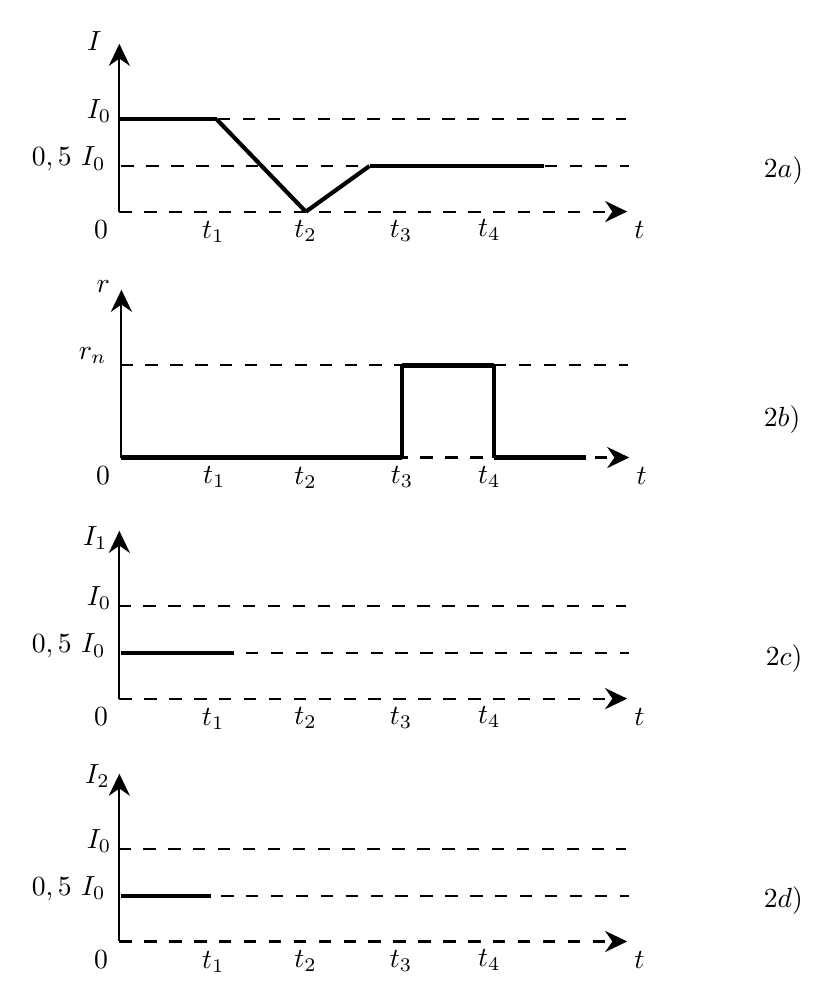
\begin{tikzpicture}[x=0.75pt,y=0.75pt,yscale=-1,xscale=1]
%uncomment if require: \path (0,506); %set diagram left start at 0, and has height of 506

%Straight Lines [id:da9338316650867005] 
\draw    (150,98) -- (150,20.17) ;
\draw [shift={(150,17.17)}, rotate = 450] [fill={rgb, 255:red, 0; green, 0; blue, 0 }  ][line width=0.08]  [draw opacity=0] (10.72,-5.15) -- (0,0) -- (10.72,5.15) -- (7.12,0) -- cycle    ;
%Straight Lines [id:da17632904655182458] 
\draw  [dash pattern={on 4.5pt off 4.5pt}]  (150,98) -- (391.67,98) ;
\draw [shift={(394.67,98)}, rotate = 180] [fill={rgb, 255:red, 0; green, 0; blue, 0 }  ][line width=0.08]  [draw opacity=0] (10.72,-5.15) -- (0,0) -- (10.72,5.15) -- (7.12,0) -- cycle    ;
%Straight Lines [id:da26463273704881884] 
\draw  [dash pattern={on 4.5pt off 4.5pt}]  (149.5,53.5) -- (394.17,53.5) ;
%Straight Lines [id:da15829977506592519] 
\draw  [dash pattern={on 4.5pt off 4.5pt}]  (151,76) -- (395.67,76) ;
%Straight Lines [id:da8291321619061571] 
\draw [line width=1.5]    (149.5,53.5) -- (196.83,53.5) ;
%Straight Lines [id:da3542938318151021] 
\draw [line width=1.5]    (196.83,53.5) -- (239.83,98.08) ;
%Straight Lines [id:da5570891195362955] 
\draw [line width=1.5]    (270.52,76.05) -- (239.83,98.08) ;
%Straight Lines [id:da6645035327577644] 
\draw    (151,216.5) -- (151,138.67) ;
\draw [shift={(151,135.67)}, rotate = 450] [fill={rgb, 255:red, 0; green, 0; blue, 0 }  ][line width=0.08]  [draw opacity=0] (10.72,-5.15) -- (0,0) -- (10.72,5.15) -- (7.12,0) -- cycle    ;
%Straight Lines [id:da7960419233770377] 
\draw  [dash pattern={on 4.5pt off 4.5pt}]  (151,216.5) -- (392.67,216.5) ;
\draw [shift={(395.67,216.5)}, rotate = 180] [fill={rgb, 255:red, 0; green, 0; blue, 0 }  ][line width=0.08]  [draw opacity=0] (10.72,-5.15) -- (0,0) -- (10.72,5.15) -- (7.12,0) -- cycle    ;
%Straight Lines [id:da796871502960965] 
\draw  [dash pattern={on 4.5pt off 4.5pt}]  (150.5,172) -- (395.17,172) ;
%Straight Lines [id:da7080780935391358] 
\draw [line width=1.5]    (151,216.5) -- (286,216.5) ;
%Straight Lines [id:da08584300148374124] 
\draw [line width=1.5]    (286,172.17) -- (286,216.5) ;
%Straight Lines [id:da296648831179557] 
\draw [line width=1.5]    (286,172.17) -- (330.5,172.17) ;
%Straight Lines [id:da8694451012709175] 
\draw [line width=1.5]    (330.5,172.17) -- (330.5,216.5) ;
%Straight Lines [id:da07268917107145612] 
\draw [line width=1.5]    (330.5,216.5) -- (375,216.5) ;
%Straight Lines [id:da06567669590801972] 
\draw [line width=1.5]    (270.52,76.05) -- (354.6,76.05) ;
%Straight Lines [id:da1786863319032621] 
\draw    (150,332.67) -- (150,254.83) ;
\draw [shift={(150,251.83)}, rotate = 450] [fill={rgb, 255:red, 0; green, 0; blue, 0 }  ][line width=0.08]  [draw opacity=0] (10.72,-5.15) -- (0,0) -- (10.72,5.15) -- (7.12,0) -- cycle    ;
%Straight Lines [id:da6712184904672815] 
\draw  [dash pattern={on 4.5pt off 4.5pt}]  (150,332.67) -- (391.67,332.67) ;
\draw [shift={(394.67,332.67)}, rotate = 180] [fill={rgb, 255:red, 0; green, 0; blue, 0 }  ][line width=0.08]  [draw opacity=0] (10.72,-5.15) -- (0,0) -- (10.72,5.15) -- (7.12,0) -- cycle    ;
%Straight Lines [id:da7600334011864698] 
\draw  [dash pattern={on 4.5pt off 4.5pt}]  (149.5,288.17) -- (394.17,288.17) ;
%Straight Lines [id:da3620609296290802] 
\draw  [dash pattern={on 4.5pt off 4.5pt}]  (151,310.67) -- (395.67,310.67) ;
%Straight Lines [id:da8318661799802061] 
\draw [line width=1.5]    (151,310.67) -- (205,310.67) ;
%Straight Lines [id:da47464332085768346] 
\draw    (150,449.67) -- (150,371.83) ;
\draw [shift={(150,368.83)}, rotate = 450] [fill={rgb, 255:red, 0; green, 0; blue, 0 }  ][line width=0.08]  [draw opacity=0] (10.72,-5.15) -- (0,0) -- (10.72,5.15) -- (7.12,0) -- cycle    ;
%Straight Lines [id:da6122409938063353] 
\draw  [dash pattern={on 4.5pt off 4.5pt}]  (150,449.67) -- (391.67,449.67) ;
\draw [shift={(394.67,449.67)}, rotate = 180] [fill={rgb, 255:red, 0; green, 0; blue, 0 }  ][line width=0.08]  [draw opacity=0] (10.72,-5.15) -- (0,0) -- (10.72,5.15) -- (7.12,0) -- cycle    ;
%Straight Lines [id:da3106491168712966] 
\draw  [dash pattern={on 4.5pt off 4.5pt}]  (149.5,405.17) -- (394.17,405.17) ;
%Straight Lines [id:da7638398486706961] 
\draw  [dash pattern={on 4.5pt off 4.5pt}]  (151,427.67) -- (395.67,427.67) ;
%Straight Lines [id:da02984470672902484] 
\draw [line width=1.5]    (151,427.67) -- (194,427.67) ;

% Text Node
\draw (133,9.9) node [anchor=north west][inner sep=0.75pt]    {$I$};
% Text Node
\draw (396.67,101.4) node [anchor=north west][inner sep=0.75pt]    {$t$};
% Text Node
\draw (106.33,65.4) node [anchor=north west][inner sep=0.75pt]    {$0,5\ I_{0}$};
% Text Node
\draw (132.83,42.4) node [anchor=north west][inner sep=0.75pt]    {$I_{0}$};
% Text Node
\draw (136.33,100.9) node [anchor=north west][inner sep=0.75pt]    {$0$};
% Text Node
\draw (188.33,101.4) node [anchor=north west][inner sep=0.75pt]    {$t_{1}$};
% Text Node
\draw (232.83,100.9) node [anchor=north west][inner sep=0.75pt]    {$t_{2}$};
% Text Node
\draw (278.83,100.9) node [anchor=north west][inner sep=0.75pt]    {$t_{3}$};
% Text Node
\draw (321.33,100.4) node [anchor=north west][inner sep=0.75pt]    {$t_{4}$};
% Text Node
\draw (137.5,129.9) node [anchor=north west][inner sep=0.75pt]    {$r$};
% Text Node
\draw (397.67,219.9) node [anchor=north west][inner sep=0.75pt]    {$t$};
% Text Node
\draw (137.33,219.4) node [anchor=north west][inner sep=0.75pt]    {$0$};
% Text Node
\draw (188.83,219.4) node [anchor=north west][inner sep=0.75pt]    {$t_{1}$};
% Text Node
\draw (232.83,219.9) node [anchor=north west][inner sep=0.75pt]    {$t_{2}$};
% Text Node
\draw (279.33,219.4) node [anchor=north west][inner sep=0.75pt]    {$t_{3}$};
% Text Node
\draw (321.33,219.4) node [anchor=north west][inner sep=0.75pt]    {$t_{4}$};
% Text Node
\draw (131,248.07) node [anchor=north west][inner sep=0.75pt]    {$I_{1}$};
% Text Node
\draw (396.67,336.07) node [anchor=north west][inner sep=0.75pt]    {$t$};
% Text Node
\draw (106.33,300.07) node [anchor=north west][inner sep=0.75pt]    {$0,5\ I_{0}$};
% Text Node
\draw (132.83,277.07) node [anchor=north west][inner sep=0.75pt]    {$I_{0}$};
% Text Node
\draw (136.33,335.57) node [anchor=north west][inner sep=0.75pt]    {$0$};
% Text Node
\draw (188.33,336.07) node [anchor=north west][inner sep=0.75pt]    {$t_{1}$};
% Text Node
\draw (232.83,335.57) node [anchor=north west][inner sep=0.75pt]    {$t_{2}$};
% Text Node
\draw (278.83,335.57) node [anchor=north west][inner sep=0.75pt]    {$t_{3}$};
% Text Node
\draw (321.33,335.07) node [anchor=north west][inner sep=0.75pt]    {$t_{4}$};
% Text Node
\draw (132,363.07) node [anchor=north west][inner sep=0.75pt]    {$I_{2}$};
% Text Node
\draw (396.67,453.07) node [anchor=north west][inner sep=0.75pt]    {$t$};
% Text Node
\draw (106.33,417.07) node [anchor=north west][inner sep=0.75pt]    {$0,5\ I_{0}$};
% Text Node
\draw (132.83,394.07) node [anchor=north west][inner sep=0.75pt]    {$I_{0}$};
% Text Node
\draw (136.33,452.57) node [anchor=north west][inner sep=0.75pt]    {$0$};
% Text Node
\draw (188.33,453.07) node [anchor=north west][inner sep=0.75pt]    {$t_{1}$};
% Text Node
\draw (232.83,452.57) node [anchor=north west][inner sep=0.75pt]    {$t_{2}$};
% Text Node
\draw (278.83,452.57) node [anchor=north west][inner sep=0.75pt]    {$t_{3}$};
% Text Node
\draw (321.33,452.07) node [anchor=north west][inner sep=0.75pt]    {$t_{4}$};
% Text Node
\draw (459,70.07) node [anchor=north west][inner sep=0.75pt]    {$2a)$};
% Text Node
\draw (459,190.07) node [anchor=north west][inner sep=0.75pt]    {$2b)$};
% Text Node
\draw (460,305.07) node [anchor=north west][inner sep=0.75pt]    {$2c)$};
% Text Node
\draw (459,421.73) node [anchor=north west][inner sep=0.75pt]    {$2d)$};
% Text Node
\draw (129,162.07) node [anchor=north west][inner sep=0.75pt]    {$r_{n}$};
\end{tikzpicture}

    \end{center}
    \item Giả sử ta đóng công tắc nguồn điện $({K})$ ở thời điểm ${t}=0$, khi $r = 0$, ${I}_{1} = 0$ và $R = 7,5 ~\Omega$, dòng điện tổng cộng $I$ là $0,5 \mathrm{~A}$. Giữ ${K}$ tiếp tục đóng, và thay đổi điện trở ${r}$ của ngắt điện siêu dẫn như trên hình $3b)$. Vẽ đồ thị phụ thuộc theo thời gian của ${I}, {I}_{1}$ và ${I}_{2}$ vào các hình $3a), 3c)$ và $3d)$).
  \begin{center}
      

\tikzset{every picture/.style={line width=0.75pt}} %set default line width to 0.75pt        

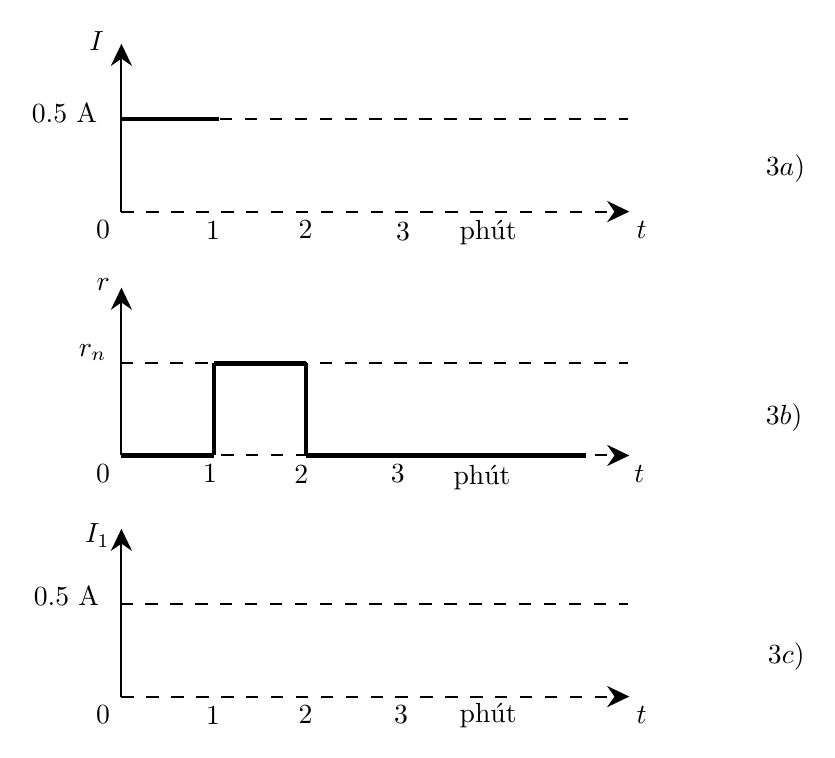
\begin{tikzpicture}[x=0.75pt,y=0.75pt,yscale=-1,xscale=1]
%uncomment if require: \path (0,526); %set diagram left start at 0, and has height of 526

%Straight Lines [id:da8557731562625317] 
\draw    (166,127.33) -- (166,49.5) ;
\draw [shift={(166,46.5)}, rotate = 90] [fill={rgb, 255:red, 0; green, 0; blue, 0 }  ][line width=0.08]  [draw opacity=0] (10.72,-5.15) -- (0,0) -- (10.72,5.15) -- (7.12,0) -- cycle    ;
%Straight Lines [id:da6510706798316066] 
\draw  [dash pattern={on 4.5pt off 4.5pt}]  (166,127.33) -- (407.67,127.33) ;
\draw [shift={(410.67,127.33)}, rotate = 180] [fill={rgb, 255:red, 0; green, 0; blue, 0 }  ][line width=0.08]  [draw opacity=0] (10.72,-5.15) -- (0,0) -- (10.72,5.15) -- (7.12,0) -- cycle    ;
%Straight Lines [id:da666633706117616] 
\draw  [dash pattern={on 4.5pt off 4.5pt}]  (165.5,82.83) -- (410.17,82.83) ;
%Straight Lines [id:da5850115538474359] 
\draw [line width=1.5]    (165.5,82.83) -- (212.83,82.83) ;
%Straight Lines [id:da44496516069002867] 
\draw    (166,244.83) -- (166,167) ;
\draw [shift={(166,164)}, rotate = 90] [fill={rgb, 255:red, 0; green, 0; blue, 0 }  ][line width=0.08]  [draw opacity=0] (10.72,-5.15) -- (0,0) -- (10.72,5.15) -- (7.12,0) -- cycle    ;
%Straight Lines [id:da14799723112305774] 
\draw  [dash pattern={on 4.5pt off 4.5pt}]  (166,244.83) -- (407.67,244.83) ;
\draw [shift={(410.67,244.83)}, rotate = 180] [fill={rgb, 255:red, 0; green, 0; blue, 0 }  ][line width=0.08]  [draw opacity=0] (10.72,-5.15) -- (0,0) -- (10.72,5.15) -- (7.12,0) -- cycle    ;
%Straight Lines [id:da006799380163398316] 
\draw  [dash pattern={on 4.5pt off 4.5pt}]  (165.5,200.33) -- (410.17,200.33) ;
%Straight Lines [id:da2320678379444503] 
\draw [line width=1.5]    (255,244.83) -- (390,244.83) ;
%Straight Lines [id:da4301475681339564] 
\draw [line width=1.5]    (210.5,200.5) -- (210.5,244.83) ;
%Straight Lines [id:da9665721217307168] 
\draw [line width=1.5]    (210.5,200.5) -- (255,200.5) ;
%Straight Lines [id:da5683091916500405] 
\draw [line width=1.5]    (255,200.5) -- (255,244.83) ;
%Straight Lines [id:da9250807216737327] 
\draw [line width=1.5]    (166,244.83) -- (210.5,244.83) ;
%Straight Lines [id:da8050523641167511] 
\draw    (166,361) -- (166,283.17) ;
\draw [shift={(166,280.17)}, rotate = 90] [fill={rgb, 255:red, 0; green, 0; blue, 0 }  ][line width=0.08]  [draw opacity=0] (10.72,-5.15) -- (0,0) -- (10.72,5.15) -- (7.12,0) -- cycle    ;
%Straight Lines [id:da6419178874081422] 
\draw  [dash pattern={on 4.5pt off 4.5pt}]  (166,361) -- (407.67,361) ;
\draw [shift={(410.67,361)}, rotate = 180] [fill={rgb, 255:red, 0; green, 0; blue, 0 }  ][line width=0.08]  [draw opacity=0] (10.72,-5.15) -- (0,0) -- (10.72,5.15) -- (7.12,0) -- cycle    ;
%Straight Lines [id:da39537108664158516] 
\draw  [dash pattern={on 4.5pt off 4.5pt}]  (165.5,316.5) -- (410.17,316.5) ;

% Text Node
\draw (149,39.23) node [anchor=north west][inner sep=0.75pt]    {$I$};
% Text Node
\draw (412.67,130.73) node [anchor=north west][inner sep=0.75pt]    {$t$};
% Text Node
\draw (121.33,73.73) node [anchor=north west][inner sep=0.75pt]    {$0.5\ \mathrm{A}$};
% Text Node
\draw (152.33,130.23) node [anchor=north west][inner sep=0.75pt]    {$0$};
% Text Node
\draw (205.33,130.73) node [anchor=north west][inner sep=0.75pt]    {$1$};
% Text Node
\draw (249.83,130.23) node [anchor=north west][inner sep=0.75pt]    {$2$};
% Text Node
\draw (296.83,131.23) node [anchor=north west][inner sep=0.75pt]    {$3$};
% Text Node
\draw (152.5,158.23) node [anchor=north west][inner sep=0.75pt]    {$r$};
% Text Node
\draw (411.67,248.23) node [anchor=north west][inner sep=0.75pt]    {$t$};
% Text Node
\draw (152.33,247.73) node [anchor=north west][inner sep=0.75pt]    {$0$};
% Text Node
\draw (203.83,247.73) node [anchor=north west][inner sep=0.75pt]    {$1$};
% Text Node
\draw (247.83,248.23) node [anchor=north west][inner sep=0.75pt]    {$2$};
% Text Node
\draw (294.33,247.73) node [anchor=north west][inner sep=0.75pt]    {$3$};
% Text Node
\draw (147,276.4) node [anchor=north west][inner sep=0.75pt]    {$I_{1}$};
% Text Node
\draw (412.67,364.4) node [anchor=north west][inner sep=0.75pt]    {$t$};
% Text Node
\draw (122.33,306.4) node [anchor=north west][inner sep=0.75pt]    {$0.5\ \mathrm{A}$};
% Text Node
\draw (152.33,363.9) node [anchor=north west][inner sep=0.75pt]    {$0$};
% Text Node
\draw (205.33,364.4) node [anchor=north west][inner sep=0.75pt]    {$1$};
% Text Node
\draw (249.83,363.9) node [anchor=north west][inner sep=0.75pt]    {$2$};
% Text Node
\draw (295.83,363.9) node [anchor=north west][inner sep=0.75pt]    {$3$};
% Text Node
\draw (475,98.4) node [anchor=north west][inner sep=0.75pt]    {$3a)$};
% Text Node
\draw (475,218.4) node [anchor=north west][inner sep=0.75pt]    {$3b)$};
% Text Node
\draw (476,333.4) node [anchor=north west][inner sep=0.75pt]    {$3c)$};
% Text Node
\draw (324.5,247.83) node [anchor=north west][inner sep=0.75pt]   [align=left] {phút};
% Text Node
\draw (327.5,129.83) node [anchor=north west][inner sep=0.75pt]   [align=left] {phút};
% Text Node
\draw (327.5,362.83) node [anchor=north west][inner sep=0.75pt]   [align=left] {phút};
% Text Node
\draw (144,189.9) node [anchor=north west][inner sep=0.75pt]    {$r_{n}$};


\end{tikzpicture}

  \end{center}  
   \begin{center}
       

\tikzset{every picture/.style={line width=0.75pt}} %set default line width to 0.75pt        

\begin{tikzpicture}[x=0.75pt,y=0.75pt,yscale=-1,xscale=1]
%uncomment if require: \path (0,526); %set diagram left start at 0, and has height of 526

%Straight Lines [id:da42971951892552873] 
\draw    (174,244.17) -- (174,166.33) ;
\draw [shift={(174,163.33)}, rotate = 90] [fill={rgb, 255:red, 0; green, 0; blue, 0 }  ][line width=0.08]  [draw opacity=0] (10.72,-5.15) -- (0,0) -- (10.72,5.15) -- (7.12,0) -- cycle    ;
%Straight Lines [id:da7911706656308835] 
\draw  [dash pattern={on 4.5pt off 4.5pt}]  (174,244.17) -- (415.67,244.17) ;
\draw [shift={(418.67,244.17)}, rotate = 180] [fill={rgb, 255:red, 0; green, 0; blue, 0 }  ][line width=0.08]  [draw opacity=0] (10.72,-5.15) -- (0,0) -- (10.72,5.15) -- (7.12,0) -- cycle    ;
%Straight Lines [id:da7063750104800608] 
\draw  [dash pattern={on 4.5pt off 4.5pt}]  (173.5,199.67) -- (418.17,199.67) ;

% Text Node
\draw (156,157.57) node [anchor=north west][inner sep=0.75pt]    {$I_{2}$};
% Text Node
\draw (420.67,247.57) node [anchor=north west][inner sep=0.75pt]    {$t$};
% Text Node
\draw (129.33,190.57) node [anchor=north west][inner sep=0.75pt]    {$0.5\ \mathrm{A}$};
% Text Node
\draw (160.33,247.07) node [anchor=north west][inner sep=0.75pt]    {$0$};
% Text Node
\draw (213.33,247.57) node [anchor=north west][inner sep=0.75pt]    {$1$};
% Text Node
\draw (257.83,247.07) node [anchor=north west][inner sep=0.75pt]    {$2$};
% Text Node
\draw (303.83,247.07) node [anchor=north west][inner sep=0.75pt]    {$3$};
% Text Node
\draw (483,216.23) node [anchor=north west][inner sep=0.75pt]    {$3d)$};
% Text Node
\draw (336.5,247) node [anchor=north west][inner sep=0.75pt]   [align=left] {phút};


\end{tikzpicture}

   \end{center} 
    
    
  
    \item Khi ở trạng thái thường, ta chỉ  được phép cho dòng điện nhỏ hơn $0.5 \mathrm{~A}$ chạy qua ngắt điện siêu dẫn, với dòng lớn hơn nó sẽ bị cháy. Giả sử nam châm siêu dẫn đang hoạt động ở chế độ vĩnh cửu, nghĩa là ${I}=0$ và ${I}_{1}={i}_{1}$ (lấy là $20 \mathrm{~A}), {I}_{2} = -{i}_{1}$ như hình $4$, trong khoảng thời gian từ ${t}=0$ đến ${t} = 3$ phút. Nếu ta muốn ngừng thí nghiệm lại bằng cách giảm dòng qua nam châm đến không, thì ta phải làm thế nào? Công việc phải thực hiện qua nhiều bước. Hãy vẽ các thay đổi của $I$, $r, I_{1}$ và $I_{2}$ vào hình $4)$.
    \begin{center}


\tikzset{every picture/.style={line width=0.75pt}} %set default line width to 0.75pt        

\begin{tikzpicture}[x=0.75pt,y=0.75pt,yscale=-1,xscale=1]
%uncomment if require: \path (0,602); %set diagram left start at 0, and has height of 602

%Straight Lines [id:da9412961228831267] 
\draw  [dash pattern={on 4.5pt off 4.5pt}]  (169.5,456.33) -- (449.5,456.33) ;
%Straight Lines [id:da5070998173179793] 
\draw  [dash pattern={on 4.5pt off 4.5pt}]  (169.5,222.17) -- (449.5,222.17) ;
%Straight Lines [id:da6363246798171784] 
\draw    (170,149.17) -- (170,71.33) ;
\draw [shift={(170,68.33)}, rotate = 450] [fill={rgb, 255:red, 0; green, 0; blue, 0 }  ][line width=0.08]  [draw opacity=0] (10.72,-5.15) -- (0,0) -- (10.72,5.15) -- (7.12,0) -- cycle    ;
%Straight Lines [id:da3253706306616817] 
\draw  [dash pattern={on 4.5pt off 4.5pt}]  (170,149.17) -- (447,149.17) ;
\draw [shift={(450,149.17)}, rotate = 180] [fill={rgb, 255:red, 0; green, 0; blue, 0 }  ][line width=0.08]  [draw opacity=0] (10.72,-5.15) -- (0,0) -- (10.72,5.15) -- (7.12,0) -- cycle    ;
%Straight Lines [id:da7693126819180351] 
\draw [line width=1.5]    (170,149.17) -- (215,149.17) ;
%Straight Lines [id:da805723798270102] 
\draw    (170,266.67) -- (170,188.83) ;
\draw [shift={(170,185.83)}, rotate = 450] [fill={rgb, 255:red, 0; green, 0; blue, 0 }  ][line width=0.08]  [draw opacity=0] (10.72,-5.15) -- (0,0) -- (10.72,5.15) -- (7.12,0) -- cycle    ;
%Straight Lines [id:da22914575324438813] 
\draw [line width=1.5]    (170,266.67) -- (214.5,266.67) ;
%Straight Lines [id:da5551158302590982] 
\draw  [dash pattern={on 4.5pt off 4.5pt}]  (170,266.67) -- (447,266.67) ;
\draw [shift={(450,266.67)}, rotate = 180] [fill={rgb, 255:red, 0; green, 0; blue, 0 }  ][line width=0.08]  [draw opacity=0] (10.72,-5.15) -- (0,0) -- (10.72,5.15) -- (7.12,0) -- cycle    ;
%Straight Lines [id:da8640658280353841] 
\draw    (170,381.83) -- (170,304) ;
\draw [shift={(170,301)}, rotate = 450] [fill={rgb, 255:red, 0; green, 0; blue, 0 }  ][line width=0.08]  [draw opacity=0] (10.72,-5.15) -- (0,0) -- (10.72,5.15) -- (7.12,0) -- cycle    ;
%Straight Lines [id:da5591763640761813] 
\draw  [dash pattern={on 4.5pt off 4.5pt}]  (170,381.83) -- (447,381.83) ;
\draw [shift={(450,381.83)}, rotate = 180] [fill={rgb, 255:red, 0; green, 0; blue, 0 }  ][line width=0.08]  [draw opacity=0] (10.72,-5.15) -- (0,0) -- (10.72,5.15) -- (7.12,0) -- cycle    ;
%Straight Lines [id:da664324058970788] 
\draw [line width=1.5]    (169.5,337.33) -- (216.83,337.33) ;
%Straight Lines [id:da17884525517541539] 
\draw    (170,562.67) -- (170,423) ;
\draw [shift={(170,420)}, rotate = 450] [fill={rgb, 255:red, 0; green, 0; blue, 0 }  ][line width=0.08]  [draw opacity=0] (10.72,-5.15) -- (0,0) -- (10.72,5.15) -- (7.12,0) -- cycle    ;
%Straight Lines [id:da6997362711536046] 
\draw  [dash pattern={on 4.5pt off 4.5pt}]  (170,500.83) -- (447,500.83) ;
\draw [shift={(450,500.83)}, rotate = 180] [fill={rgb, 255:red, 0; green, 0; blue, 0 }  ][line width=0.08]  [draw opacity=0] (10.72,-5.15) -- (0,0) -- (10.72,5.15) -- (7.12,0) -- cycle    ;
%Straight Lines [id:da989227080197443] 
\draw [line width=1.5]    (169.5,543.33) -- (216.83,543.33) ;
%Straight Lines [id:da21364527821825585] 
\draw  [dash pattern={on 4.5pt off 4.5pt}]  (170,108.75) -- (450,108.75) ;
%Straight Lines [id:da011102150036357727] 
\draw  [dash pattern={on 4.5pt off 4.5pt}]  (169.5,337.33) -- (449.5,337.33) ;
%Straight Lines [id:da7713401469398977] 
\draw  [dash pattern={on 4.5pt off 4.5pt}]  (169.5,543.33) -- (449.5,543.33) ;

% Text Node
\draw (153,61.07) node [anchor=north west][inner sep=0.75pt]    {$I$};
% Text Node
\draw (452,152.57) node [anchor=north west][inner sep=0.75pt]    {$t$};
% Text Node
\draw (128.33,95.57) node [anchor=north west][inner sep=0.75pt]    {$20\ \mathrm{A}$};
% Text Node
\draw (156.33,152.07) node [anchor=north west][inner sep=0.75pt]    {$0$};
% Text Node
\draw (209.33,152.57) node [anchor=north west][inner sep=0.75pt]    {$3$};
% Text Node
\draw (253.83,152.07) node [anchor=north west][inner sep=0.75pt]    {$6$};
% Text Node
\draw (300.83,153.07) node [anchor=north west][inner sep=0.75pt]    {$9$};
% Text Node
\draw (156.5,180.07) node [anchor=north west][inner sep=0.75pt]    {$r$};
% Text Node
\draw (156.33,269.57) node [anchor=north west][inner sep=0.75pt]    {$0$};
% Text Node
\draw (479,120.23) node [anchor=north west][inner sep=0.75pt]    {$4a)$};
% Text Node
\draw (479,240.23) node [anchor=north west][inner sep=0.75pt]    {$4b)$};
% Text Node
\draw (480,355.23) node [anchor=north west][inner sep=0.75pt]    {$4c)$};
% Text Node
\draw (479,490.9) node [anchor=north west][inner sep=0.75pt]    {$4d)$};
% Text Node
\draw (384.5,151.67) node [anchor=north west][inner sep=0.75pt]   [align=left] {phút};
% Text Node
\draw (341,151.4) node [anchor=north west][inner sep=0.75pt]    {$12$};
% Text Node
\draw (452,270.57) node [anchor=north west][inner sep=0.75pt]    {$t$};
% Text Node
\draw (209.33,269.57) node [anchor=north west][inner sep=0.75pt]    {$3$};
% Text Node
\draw (253.83,269.07) node [anchor=north west][inner sep=0.75pt]    {$6$};
% Text Node
\draw (300.83,269.07) node [anchor=north west][inner sep=0.75pt]    {$9$};
% Text Node
\draw (384.5,268.67) node [anchor=north west][inner sep=0.75pt]   [align=left] {phút};
% Text Node
\draw (341,269.4) node [anchor=north west][inner sep=0.75pt]    {$12$};
% Text Node
\draw (150,293.73) node [anchor=north west][inner sep=0.75pt]    {$I_{1}$};
% Text Node
\draw (452,385.23) node [anchor=north west][inner sep=0.75pt]    {$t$};
% Text Node
\draw (129.33,328.23) node [anchor=north west][inner sep=0.75pt]    {$20\ \mathrm{A}$};
% Text Node
\draw (156.33,384.73) node [anchor=north west][inner sep=0.75pt]    {$0$};
% Text Node
\draw (209.33,385.23) node [anchor=north west][inner sep=0.75pt]    {$3$};
% Text Node
\draw (253.83,384.73) node [anchor=north west][inner sep=0.75pt]    {$6$};
% Text Node
\draw (300.83,385.73) node [anchor=north west][inner sep=0.75pt]    {$9$};
% Text Node
\draw (384.5,384.33) node [anchor=north west][inner sep=0.75pt]   [align=left] {phút};
% Text Node
\draw (341,384.07) node [anchor=north west][inner sep=0.75pt]    {$12$};
% Text Node
\draw (150,412.73) node [anchor=north west][inner sep=0.75pt]    {$I_{2}$};
% Text Node
\draw (452,504.23) node [anchor=north west][inner sep=0.75pt]    {$t$};
% Text Node
\draw (128.33,446.23) node [anchor=north west][inner sep=0.75pt]    {$20\ \mathrm{A}$};
% Text Node
\draw (156.33,503.73) node [anchor=north west][inner sep=0.75pt]    {$0$};
% Text Node
\draw (209.33,504.23) node [anchor=north west][inner sep=0.75pt]    {$3$};
% Text Node
\draw (253.83,503.73) node [anchor=north west][inner sep=0.75pt]    {$6$};
% Text Node
\draw (300.83,504.73) node [anchor=north west][inner sep=0.75pt]    {$9$};
% Text Node
\draw (384.5,503.33) node [anchor=north west][inner sep=0.75pt]   [align=left] {phút};
% Text Node
\draw (341,503.07) node [anchor=north west][inner sep=0.75pt]    {$12$};
% Text Node
\draw (118.33,535.23) node [anchor=north west][inner sep=0.75pt]    {$-20\ \mathrm{A}$};
% Text Node
\draw (148,210.07) node [anchor=north west][inner sep=0.75pt]    {$r_{n}$};
\end{tikzpicture}
    \end{center}
    \item Giả sử nam châm đang hoạt động ở chế độ vĩnh cửu, dòng điện là $20 \mathrm{~A}$ (từ ${t} = 0$ đến ${t} = 3$ phút xem hình $5$ ). Làm thế nào có thể tăng dòng ở chế độ vĩnh cửu lên $30 \mathrm{~A}$. Vẽ trả lời lên hình $5)$.
    \begin{center}


\tikzset{every picture/.style={line width=0.75pt}} %set default line width to 0.75pt        

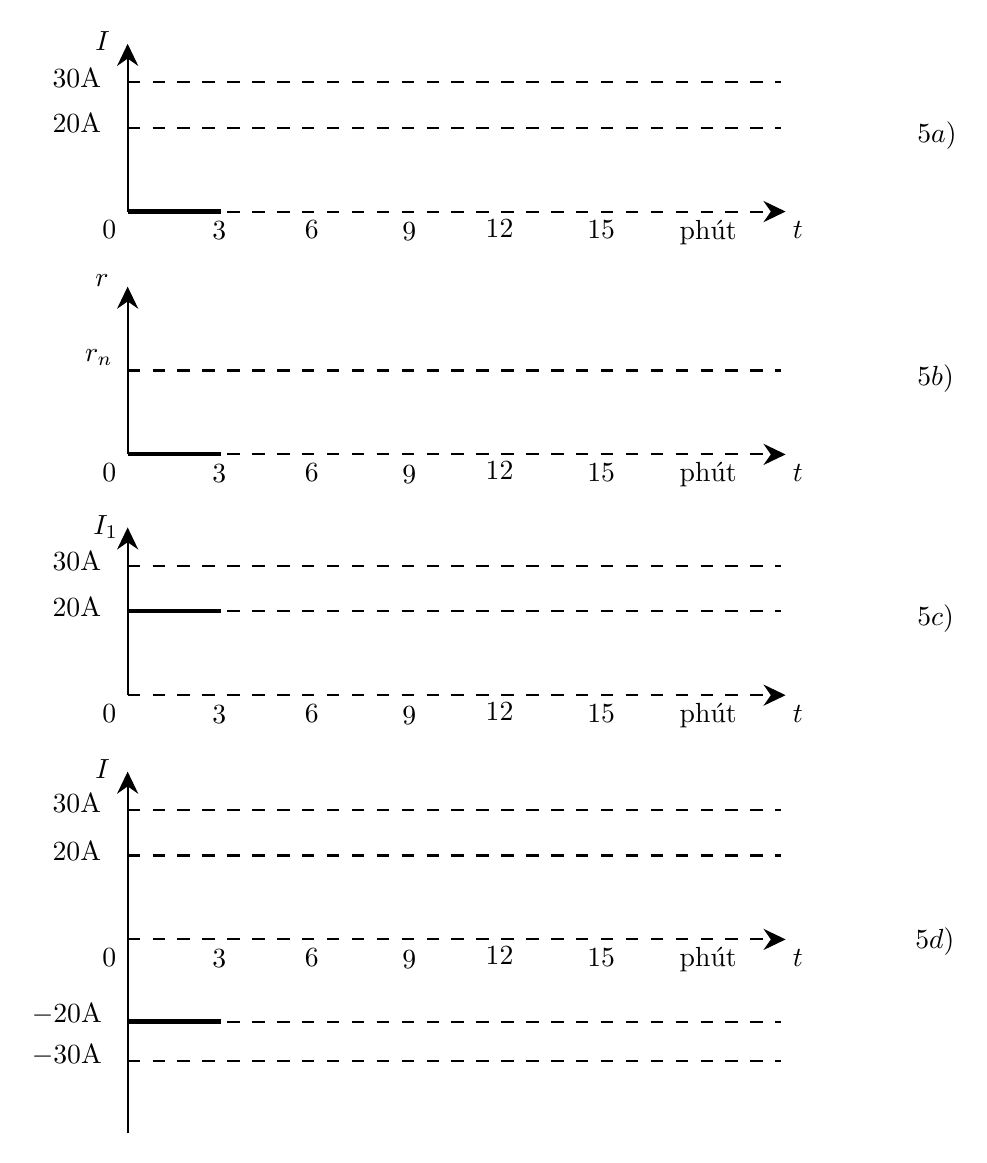
\begin{tikzpicture}[x=0.75pt,y=0.75pt,yscale=-1,xscale=1]
%uncomment if require: \path (0,602); %set diagram left start at 0, and has height of 602

%Straight Lines [id:da08002772457635476] 
\draw    (150,116.5) -- (150,38.67) ;
\draw [shift={(150,35.67)}, rotate = 450] [fill={rgb, 255:red, 0; green, 0; blue, 0 }  ][line width=0.08]  [draw opacity=0] (10.72,-5.15) -- (0,0) -- (10.72,5.15) -- (7.12,0) -- cycle    ;
%Straight Lines [id:da21657729261520298] 
\draw  [dash pattern={on 4.5pt off 4.5pt}]  (150,116.5) -- (464,116.5) ;
\draw [shift={(467,116.5)}, rotate = 180] [fill={rgb, 255:red, 0; green, 0; blue, 0 }  ][line width=0.08]  [draw opacity=0] (10.72,-5.15) -- (0,0) -- (10.72,5.15) -- (7.12,0) -- cycle    ;
%Straight Lines [id:da773982393174337] 
\draw  [dash pattern={on 4.5pt off 4.5pt}]  (150,76.08) -- (404,76.08) -- (464.75,76.08) ;
%Straight Lines [id:da599112320715431] 
\draw [line width=1.5]    (150,116.5) -- (195,116.5) ;
%Straight Lines [id:da03909998010164162] 
\draw  [dash pattern={on 4.5pt off 4.5pt}]  (150,54.08) -- (404,54.08) -- (464.75,54.08) ;
%Straight Lines [id:da16428153491268627] 
\draw    (150,233.5) -- (150,155.67) ;
\draw [shift={(150,152.67)}, rotate = 450] [fill={rgb, 255:red, 0; green, 0; blue, 0 }  ][line width=0.08]  [draw opacity=0] (10.72,-5.15) -- (0,0) -- (10.72,5.15) -- (7.12,0) -- cycle    ;
%Straight Lines [id:da5683030079759985] 
\draw  [dash pattern={on 4.5pt off 4.5pt}]  (150,233.5) -- (464,233.5) ;
\draw [shift={(467,233.5)}, rotate = 180] [fill={rgb, 255:red, 0; green, 0; blue, 0 }  ][line width=0.08]  [draw opacity=0] (10.72,-5.15) -- (0,0) -- (10.72,5.15) -- (7.12,0) -- cycle    ;
%Straight Lines [id:da08153005674363345] 
\draw  [dash pattern={on 4.5pt off 4.5pt}]  (150,193.08) -- (404,193.08) -- (464.75,193.08) ;
%Straight Lines [id:da6094322323932311] 
\draw [line width=1.5]    (150,233.5) -- (195,233.5) ;
%Straight Lines [id:da10092694263912483] 
\draw    (150,349.5) -- (150,271.67) ;
\draw [shift={(150,268.67)}, rotate = 450] [fill={rgb, 255:red, 0; green, 0; blue, 0 }  ][line width=0.08]  [draw opacity=0] (10.72,-5.15) -- (0,0) -- (10.72,5.15) -- (7.12,0) -- cycle    ;
%Straight Lines [id:da6380887399475066] 
\draw  [dash pattern={on 4.5pt off 4.5pt}]  (150,349.5) -- (464,349.5) ;
\draw [shift={(467,349.5)}, rotate = 180] [fill={rgb, 255:red, 0; green, 0; blue, 0 }  ][line width=0.08]  [draw opacity=0] (10.72,-5.15) -- (0,0) -- (10.72,5.15) -- (7.12,0) -- cycle    ;
%Straight Lines [id:da5785998322841315] 
\draw  [dash pattern={on 4.5pt off 4.5pt}]  (150,309.08) -- (404,309.08) -- (464.75,309.08) ;
%Straight Lines [id:da5687323393626402] 
\draw [line width=1.5]    (150,309.08) -- (195,309.08) ;
%Straight Lines [id:da3749723855751004] 
\draw  [dash pattern={on 4.5pt off 4.5pt}]  (150,287.08) -- (404,287.08) -- (464.75,287.08) ;
%Straight Lines [id:da25626979370832803] 
\draw    (150,560.67) -- (150,389.33) ;
\draw [shift={(150,386.33)}, rotate = 450] [fill={rgb, 255:red, 0; green, 0; blue, 0 }  ][line width=0.08]  [draw opacity=0] (10.72,-5.15) -- (0,0) -- (10.72,5.15) -- (7.12,0) -- cycle    ;
%Straight Lines [id:da18446980813227398] 
\draw  [dash pattern={on 4.5pt off 4.5pt}]  (150,467.17) -- (464,467.17) ;
\draw [shift={(467,467.17)}, rotate = 180] [fill={rgb, 255:red, 0; green, 0; blue, 0 }  ][line width=0.08]  [draw opacity=0] (10.72,-5.15) -- (0,0) -- (10.72,5.15) -- (7.12,0) -- cycle    ;
%Straight Lines [id:da047284291463099315] 
\draw  [dash pattern={on 4.5pt off 4.5pt}]  (150,426.75) -- (404,426.75) -- (464.75,426.75) ;
%Straight Lines [id:da6570814303519765] 
\draw [line width=1.5]    (150,506.75) -- (195,506.75) ;
%Straight Lines [id:da3734621981707995] 
\draw  [dash pattern={on 4.5pt off 4.5pt}]  (150,404.75) -- (404,404.75) -- (464.75,404.75) ;
%Straight Lines [id:da11516957614406942] 
\draw  [dash pattern={on 4.5pt off 4.5pt}]  (150,506.75) -- (404,506.75) -- (464.75,506.75) ;
%Straight Lines [id:da22328387762661728] 
\draw  [dash pattern={on 4.5pt off 4.5pt}]  (150,525.75) -- (404,525.75) -- (464.75,525.75) ;

% Text Node
\draw (133,28.4) node [anchor=north west][inner sep=0.75pt]    {$I$};
% Text Node
\draw (469,119.9) node [anchor=north west][inner sep=0.75pt]    {$t$};
% Text Node
\draw (112.33,67.9) node [anchor=north west][inner sep=0.75pt]    {$20\mathrm{A}$};
% Text Node
\draw (136.33,119.4) node [anchor=north west][inner sep=0.75pt]    {$0$};
% Text Node
\draw (189.33,119.9) node [anchor=north west][inner sep=0.75pt]    {$3$};
% Text Node
\draw (233.83,119.4) node [anchor=north west][inner sep=0.75pt]    {$6$};
% Text Node
\draw (280.83,120.4) node [anchor=north west][inner sep=0.75pt]    {$9$};
% Text Node
\draw (529,71.57) node [anchor=north west][inner sep=0.75pt]    {$5a)$};
% Text Node
\draw (414.5,119) node [anchor=north west][inner sep=0.75pt]   [align=left] {phút};
% Text Node
\draw (321,118.73) node [anchor=north west][inner sep=0.75pt]    {$12$};
% Text Node
\draw (370,119.4) node [anchor=north west][inner sep=0.75pt]    {$15$};
% Text Node
\draw (112.33,45.9) node [anchor=north west][inner sep=0.75pt]    {$30\mathrm{A}$};
% Text Node
\draw (133,145.4) node [anchor=north west][inner sep=0.75pt]    {$r$};
% Text Node
\draw (469,236.9) node [anchor=north west][inner sep=0.75pt]    {$t$};
% Text Node
\draw (136.33,236.4) node [anchor=north west][inner sep=0.75pt]    {$0$};
% Text Node
\draw (189.33,236.9) node [anchor=north west][inner sep=0.75pt]    {$3$};
% Text Node
\draw (233.83,236.4) node [anchor=north west][inner sep=0.75pt]    {$6$};
% Text Node
\draw (280.83,237.4) node [anchor=north west][inner sep=0.75pt]    {$9$};
% Text Node
\draw (529,188.57) node [anchor=north west][inner sep=0.75pt]    {$5b)$};
% Text Node
\draw (414.5,236) node [anchor=north west][inner sep=0.75pt]   [align=left] {phút};
% Text Node
\draw (321,235.73) node [anchor=north west][inner sep=0.75pt]    {$12$};
% Text Node
\draw (370,236.4) node [anchor=north west][inner sep=0.75pt]    {$15$};
% Text Node
\draw (132,261.4) node [anchor=north west][inner sep=0.75pt]    {$I_{1}$};
% Text Node
\draw (469,352.9) node [anchor=north west][inner sep=0.75pt]    {$t$};
% Text Node
\draw (112.33,300.9) node [anchor=north west][inner sep=0.75pt]    {$20\mathrm{A}$};
% Text Node
\draw (136.33,352.4) node [anchor=north west][inner sep=0.75pt]    {$0$};
% Text Node
\draw (189.33,352.9) node [anchor=north west][inner sep=0.75pt]    {$3$};
% Text Node
\draw (233.83,352.4) node [anchor=north west][inner sep=0.75pt]    {$6$};
% Text Node
\draw (280.83,353.4) node [anchor=north west][inner sep=0.75pt]    {$9$};
% Text Node
\draw (529,304.57) node [anchor=north west][inner sep=0.75pt]    {$5c)$};
% Text Node
\draw (414.5,352) node [anchor=north west][inner sep=0.75pt]   [align=left] {phút};
% Text Node
\draw (321,351.73) node [anchor=north west][inner sep=0.75pt]    {$12$};
% Text Node
\draw (370,352.4) node [anchor=north west][inner sep=0.75pt]    {$15$};
% Text Node
\draw (112.33,278.9) node [anchor=north west][inner sep=0.75pt]    {$30\mathrm{A}$};
% Text Node
\draw (133,379.07) node [anchor=north west][inner sep=0.75pt]    {$I$};
% Text Node
\draw (469,470.57) node [anchor=north west][inner sep=0.75pt]    {$t$};
% Text Node
\draw (112.33,418.57) node [anchor=north west][inner sep=0.75pt]    {$20\mathrm{A}$};
% Text Node
\draw (136.33,470.07) node [anchor=north west][inner sep=0.75pt]    {$0$};
% Text Node
\draw (189.33,470.57) node [anchor=north west][inner sep=0.75pt]    {$3$};
% Text Node
\draw (233.83,470.07) node [anchor=north west][inner sep=0.75pt]    {$6$};
% Text Node
\draw (280.83,471.07) node [anchor=north west][inner sep=0.75pt]    {$9$};
% Text Node
\draw (528,460.23) node [anchor=north west][inner sep=0.75pt]    {$5d)$};
% Text Node
\draw (414.5,469.67) node [anchor=north west][inner sep=0.75pt]   [align=left] {phút};
% Text Node
\draw (321,469.4) node [anchor=north west][inner sep=0.75pt]    {$12$};
% Text Node
\draw (370,470.07) node [anchor=north west][inner sep=0.75pt]    {$15$};
% Text Node
\draw (112.33,395.57) node [anchor=north west][inner sep=0.75pt]    {$30\mathrm{A}$};
% Text Node
\draw (128,181.4) node [anchor=north west][inner sep=0.75pt]    {$r_{n}$};
% Text Node
\draw (102.33,496.57) node [anchor=north west][inner sep=0.75pt]    {$-20\mathrm{A}$};
% Text Node
\draw (102.33,516.57) node [anchor=north west][inner sep=0.75pt]    {$-30\mathrm{A}$};
\end{tikzpicture}
    \end{center}
\end{enumerate}
\end{vd}
\begin{loigiai}\[\]
\begin{enumerate}[1)]
    \item 
    \begin{itemize}
        \item Với $t$ thay đổi từ $t = t_1 $ đến $t = t_3$:\\
    Vì $r = 0$ nên độ sụt thế trên nam châm $V_M = L\dfrac{\dd I_1}{\dd t} = 0$ nên
    \[\heva{I_1 &= I_1(t) = \dfrac{1}{2}I_0 \\ I_2 &= I - I_1 = I - \dfrac{1}{2}I_0}.\]
    \item Với $t$ thay đổi từ $t_3$ đến $t_4$:\\
    Vì $I_2 = 0$ tại $t = t_3$ và $I$ giữ nguyên giá trị $\dfrac{1}{2}I_0$ trong suốt thời gian sau đó. Khi $t = t_3$, $V_M = I_2r_n = 0$ nên $I_1$ và $I_2$ không đổi
    \[\heva{I_1 &= \dfrac{1}{2}I_0 \\ I_2 &= 0}.\]
    \end{itemize}
    Các kết quả được vẽ trên hình $6$.
    \begin{center}
        

\tikzset{every picture/.style={line width=0.75pt}} %set default line width to 0.75pt        

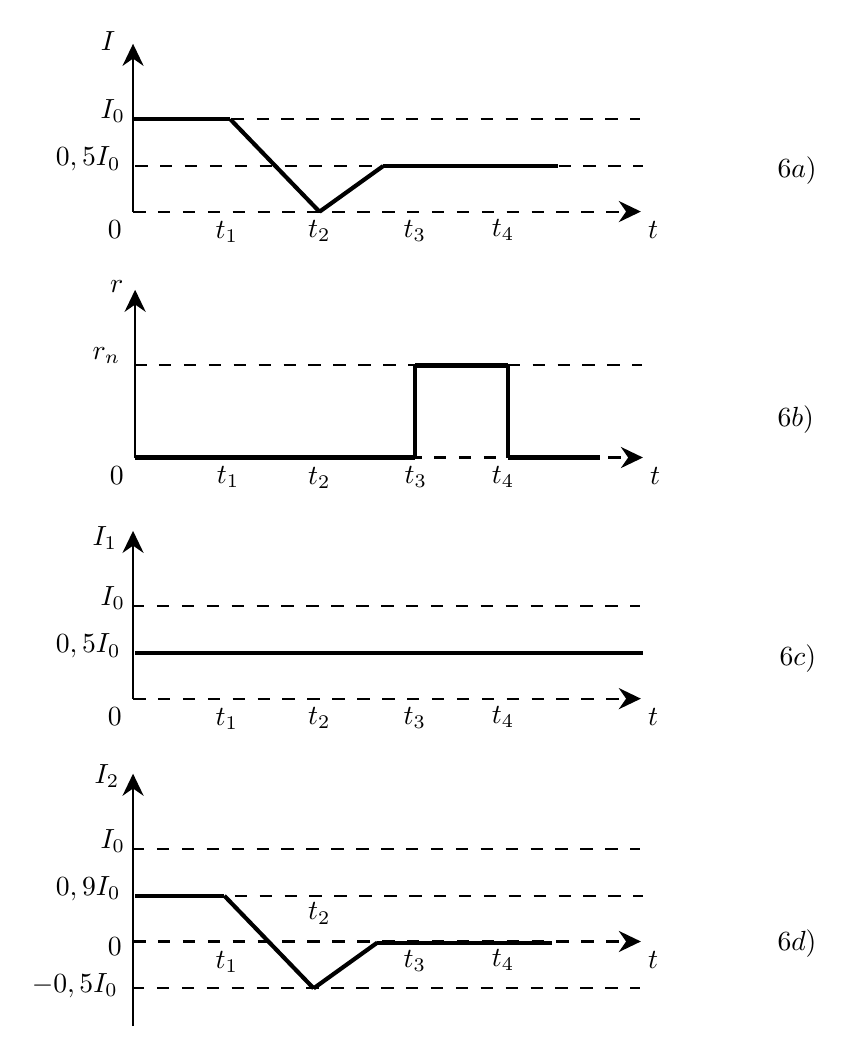
\begin{tikzpicture}[x=0.75pt,y=0.75pt,yscale=-1,xscale=1]
%uncomment if require: \path (0,576); %set diagram left start at 0, and has height of 576

%Straight Lines [id:da14930957180595983] 
\draw    (170,131.5) -- (170,53.67) ;
\draw [shift={(170,50.67)}, rotate = 450] [fill={rgb, 255:red, 0; green, 0; blue, 0 }  ][line width=0.08]  [draw opacity=0] (10.72,-5.15) -- (0,0) -- (10.72,5.15) -- (7.12,0) -- cycle    ;
%Straight Lines [id:da4124112122028407] 
\draw  [dash pattern={on 4.5pt off 4.5pt}]  (170,131.5) -- (411.67,131.5) ;
\draw [shift={(414.67,131.5)}, rotate = 180] [fill={rgb, 255:red, 0; green, 0; blue, 0 }  ][line width=0.08]  [draw opacity=0] (10.72,-5.15) -- (0,0) -- (10.72,5.15) -- (7.12,0) -- cycle    ;
%Straight Lines [id:da9794178852205824] 
\draw  [dash pattern={on 4.5pt off 4.5pt}]  (169.5,87) -- (414.17,87) ;
%Straight Lines [id:da2700423998936725] 
\draw  [dash pattern={on 4.5pt off 4.5pt}]  (171,109.5) -- (415.67,109.5) ;
%Straight Lines [id:da07994266409717654] 
\draw [line width=1.5]    (169.5,87) -- (216.83,87) ;
%Straight Lines [id:da3676328730279599] 
\draw [line width=1.5]    (216.83,87) -- (259.83,131.58) ;
%Straight Lines [id:da018807447854860992] 
\draw [line width=1.5]    (290.52,109.55) -- (259.83,131.58) ;
%Straight Lines [id:da49167658718040497] 
\draw    (171,250) -- (171,172.17) ;
\draw [shift={(171,169.17)}, rotate = 450] [fill={rgb, 255:red, 0; green, 0; blue, 0 }  ][line width=0.08]  [draw opacity=0] (10.72,-5.15) -- (0,0) -- (10.72,5.15) -- (7.12,0) -- cycle    ;
%Straight Lines [id:da813083250614121] 
\draw  [dash pattern={on 4.5pt off 4.5pt}]  (171,250) -- (412.67,250) ;
\draw [shift={(415.67,250)}, rotate = 180] [fill={rgb, 255:red, 0; green, 0; blue, 0 }  ][line width=0.08]  [draw opacity=0] (10.72,-5.15) -- (0,0) -- (10.72,5.15) -- (7.12,0) -- cycle    ;
%Straight Lines [id:da03993995848835108] 
\draw  [dash pattern={on 4.5pt off 4.5pt}]  (170.5,205.5) -- (415.17,205.5) ;
%Straight Lines [id:da5665756813629024] 
\draw [line width=1.5]    (171,250) -- (306,250) ;
%Straight Lines [id:da12031990569016249] 
\draw [line width=1.5]    (306,205.67) -- (306,250) ;
%Straight Lines [id:da4795982786470714] 
\draw [line width=1.5]    (306,205.67) -- (350.5,205.67) ;
%Straight Lines [id:da033230832098241514] 
\draw [line width=1.5]    (350.5,205.67) -- (350.5,250) ;
%Straight Lines [id:da9763619358232134] 
\draw [line width=1.5]    (350.5,250) -- (395,250) ;
%Straight Lines [id:da25285168820403325] 
\draw [line width=1.5]    (290.52,109.55) -- (374.6,109.55) ;
%Straight Lines [id:da3923545913880664] 
\draw    (170,366.17) -- (170,288.33) ;
\draw [shift={(170,285.33)}, rotate = 450] [fill={rgb, 255:red, 0; green, 0; blue, 0 }  ][line width=0.08]  [draw opacity=0] (10.72,-5.15) -- (0,0) -- (10.72,5.15) -- (7.12,0) -- cycle    ;
%Straight Lines [id:da8771404941943441] 
\draw  [dash pattern={on 4.5pt off 4.5pt}]  (170,366.17) -- (411.67,366.17) ;
\draw [shift={(414.67,366.17)}, rotate = 180] [fill={rgb, 255:red, 0; green, 0; blue, 0 }  ][line width=0.08]  [draw opacity=0] (10.72,-5.15) -- (0,0) -- (10.72,5.15) -- (7.12,0) -- cycle    ;
%Straight Lines [id:da3897149447457744] 
\draw  [dash pattern={on 4.5pt off 4.5pt}]  (169.5,321.67) -- (414.17,321.67) ;
%Straight Lines [id:da8014374144320113] 
\draw  [dash pattern={on 4.5pt off 4.5pt}]  (171,344.17) -- (415.67,344.17) ;
%Straight Lines [id:da052302555902765224] 
\draw [line width=1.5]    (171,344.17) -- (415.67,344.17) ;
%Straight Lines [id:da5481906291659824] 
\draw    (170,524) -- (170,405.33) ;
\draw [shift={(170,402.33)}, rotate = 450] [fill={rgb, 255:red, 0; green, 0; blue, 0 }  ][line width=0.08]  [draw opacity=0] (10.72,-5.15) -- (0,0) -- (10.72,5.15) -- (7.12,0) -- cycle    ;
%Straight Lines [id:da48278438795030754] 
\draw  [dash pattern={on 4.5pt off 4.5pt}]  (170,483.17) -- (411.67,483.17) ;
\draw [shift={(414.67,483.17)}, rotate = 180] [fill={rgb, 255:red, 0; green, 0; blue, 0 }  ][line width=0.08]  [draw opacity=0] (10.72,-5.15) -- (0,0) -- (10.72,5.15) -- (7.12,0) -- cycle    ;
%Straight Lines [id:da1922301980457426] 
\draw  [dash pattern={on 4.5pt off 4.5pt}]  (169.5,438.67) -- (414.17,438.67) ;
%Straight Lines [id:da3577934583777349] 
\draw  [dash pattern={on 4.5pt off 4.5pt}]  (171,461.17) -- (415.67,461.17) ;
%Straight Lines [id:da2715814333274458] 
\draw [line width=1.5]    (171,461.17) -- (196.07,461.17) -- (214,461.17) ;
%Straight Lines [id:da9780711539795166] 
\draw  [dash pattern={on 4.5pt off 4.5pt}]  (169.5,505.67) -- (283.67,505.67) -- (414.17,505.67) ;
%Straight Lines [id:da37071072164125685] 
\draw [line width=1.5]    (214,461.17) -- (257,505.75) ;
%Straight Lines [id:da014352319428391214] 
\draw [line width=1.5]    (287.69,483.71) -- (257,505.75) ;
%Straight Lines [id:da6101105759218803] 
\draw [line width=1.5]    (287.69,483.71) -- (371.77,483.71) ;

% Text Node
\draw (153,43.4) node [anchor=north west][inner sep=0.75pt]    {$I$};
% Text Node
\draw (416.67,134.9) node [anchor=north west][inner sep=0.75pt]    {$t$};
% Text Node
\draw (131.33,98.9) node [anchor=north west][inner sep=0.75pt]    {$0,5I_{0}$};
% Text Node
\draw (152.83,75.9) node [anchor=north west][inner sep=0.75pt]    {$I_{0}$};
% Text Node
\draw (156.33,134.4) node [anchor=north west][inner sep=0.75pt]    {$0$};
% Text Node
\draw (208.33,134.9) node [anchor=north west][inner sep=0.75pt]    {$t_{1}$};
% Text Node
\draw (252.83,134.4) node [anchor=north west][inner sep=0.75pt]    {$t_{2}$};
% Text Node
\draw (298.83,134.4) node [anchor=north west][inner sep=0.75pt]    {$t_{3}$};
% Text Node
\draw (341.33,133.9) node [anchor=north west][inner sep=0.75pt]    {$t_{4}$};
% Text Node
\draw (157.5,163.4) node [anchor=north west][inner sep=0.75pt]    {$r$};
% Text Node
\draw (417.67,253.4) node [anchor=north west][inner sep=0.75pt]    {$t$};
% Text Node
\draw (157.33,252.9) node [anchor=north west][inner sep=0.75pt]    {$0$};
% Text Node
\draw (208.83,252.9) node [anchor=north west][inner sep=0.75pt]    {$t_{1}$};
% Text Node
\draw (252.83,253.4) node [anchor=north west][inner sep=0.75pt]    {$t_{2}$};
% Text Node
\draw (299.33,252.9) node [anchor=north west][inner sep=0.75pt]    {$t_{3}$};
% Text Node
\draw (341.33,252.9) node [anchor=north west][inner sep=0.75pt]    {$t_{4}$};
% Text Node
\draw (149,281.57) node [anchor=north west][inner sep=0.75pt]    {$I_{1}$};
% Text Node
\draw (416.67,369.57) node [anchor=north west][inner sep=0.75pt]    {$t$};
% Text Node
\draw (131.33,333.57) node [anchor=north west][inner sep=0.75pt]    {$0,5I_{0}$};
% Text Node
\draw (152.83,310.57) node [anchor=north west][inner sep=0.75pt]    {$I_{0}$};
% Text Node
\draw (156.33,369.07) node [anchor=north west][inner sep=0.75pt]    {$0$};
% Text Node
\draw (208.33,369.57) node [anchor=north west][inner sep=0.75pt]    {$t_{1}$};
% Text Node
\draw (252.83,369.07) node [anchor=north west][inner sep=0.75pt]    {$t_{2}$};
% Text Node
\draw (298.83,369.07) node [anchor=north west][inner sep=0.75pt]    {$t_{3}$};
% Text Node
\draw (341.33,368.57) node [anchor=north west][inner sep=0.75pt]    {$t_{4}$};
% Text Node
\draw (150,396.57) node [anchor=north west][inner sep=0.75pt]    {$I_{2}$};
% Text Node
\draw (416.67,486.57) node [anchor=north west][inner sep=0.75pt]    {$t$};
% Text Node
\draw (131.33,450.57) node [anchor=north west][inner sep=0.75pt]    {$0,9I_{0}$};
% Text Node
\draw (152.83,427.57) node [anchor=north west][inner sep=0.75pt]    {$I_{0}$};
% Text Node
\draw (156.33,479.67) node [anchor=north west][inner sep=0.75pt]    {$0$};
% Text Node
\draw (208.33,486.57) node [anchor=north west][inner sep=0.75pt]    {$t_{1}$};
% Text Node
\draw (252.83,463.07) node [anchor=north west][inner sep=0.75pt]    {$t_{2}$};
% Text Node
\draw (298.83,486.07) node [anchor=north west][inner sep=0.75pt]    {$t_{3}$};
% Text Node
\draw (341.33,485.57) node [anchor=north west][inner sep=0.75pt]    {$t_{4}$};
% Text Node
\draw (479,103.57) node [anchor=north west][inner sep=0.75pt]    {$6a)$};
% Text Node
\draw (479,223.57) node [anchor=north west][inner sep=0.75pt]    {$6b)$};
% Text Node
\draw (480,338.57) node [anchor=north west][inner sep=0.75pt]    {$6c)$};
% Text Node
\draw (479,476.23) node [anchor=north west][inner sep=0.75pt]    {$6d)$};
% Text Node
\draw (149,195.57) node [anchor=north west][inner sep=0.75pt]    {$r_{n}$};
% Text Node
\draw (119.73,497.17) node [anchor=north west][inner sep=0.75pt]    {$-0,5I_{0}$};
\end{tikzpicture}
    \end{center}
    \item 
    \begin{itemize}
        \item Với $t$ thay đổi từ $t = 0$ đến $t = 1$ phút:\\
    Vì $r =0$ nên $V_M = L\dfrac{\dd I_1}{\dd t}$
    \[\rt \heva{I_1 &= I_1(0) = 0 \\ I_2 &= I - I_1 = 0,5 ~\mathrm{A} }.\]
    \item Với $t = 1$ phút, $r$ tăng đột ngột từ $0$ đến $r_n$, $I$ sẽ giảm từ $\dfrac{E}{R}$ đến $\dfrac{E}{R + r}$ một cách đột ngột, vì $I_1$ không thể thay đổi đột ngột do cảm kháng của cuộn nam châm. Với $\dfrac{E}{R} = 0,5 ~\mathrm{A}$, $R = 7.5~\Omega$ và $r_n = 5~\Omega
$, $I$ giảm còn $0,3 ~\mathrm{A}$.\\
    \item Với $t= 1$ phút đến $t = 2$ phút:\\
    $I, I_1$ và $I_2$ tiến dần đến giá trị ổn định:
    \[\heva{I &= \dfrac{E}{R} = 0,5 ~\mathrm{A}\\ I_1 &= I = 0,5 ~\mathrm{A}\\ I_2 &=0}.\]
    Hằng số thời gian \[\tau = \dfrac{L(R+r_n)}{Rr_n}.\]
    Với $L = 10~\mathrm{H}, R = 7.5~\Omega$ và $r_n = 5~\Omega$, thì $\tau = 3$ giây.
    \item Vời $t$ thay đổi từ $t = 2$ phút đến $t = 3$ phút:\\
    Vì $r = 0$, $I_1$ và $I_2$ không thay đổi, nghĩa là:
    \[\heva{I_1 &= 0,5~\mathrm{A} \\ I_2 &= 0}.\]
    \end{itemize}
    Các kết quả được vẽ trên hình $7$.
    \begin{center}
        

\tikzset{every picture/.style={line width=0.75pt}} %set default line width to 0.75pt        

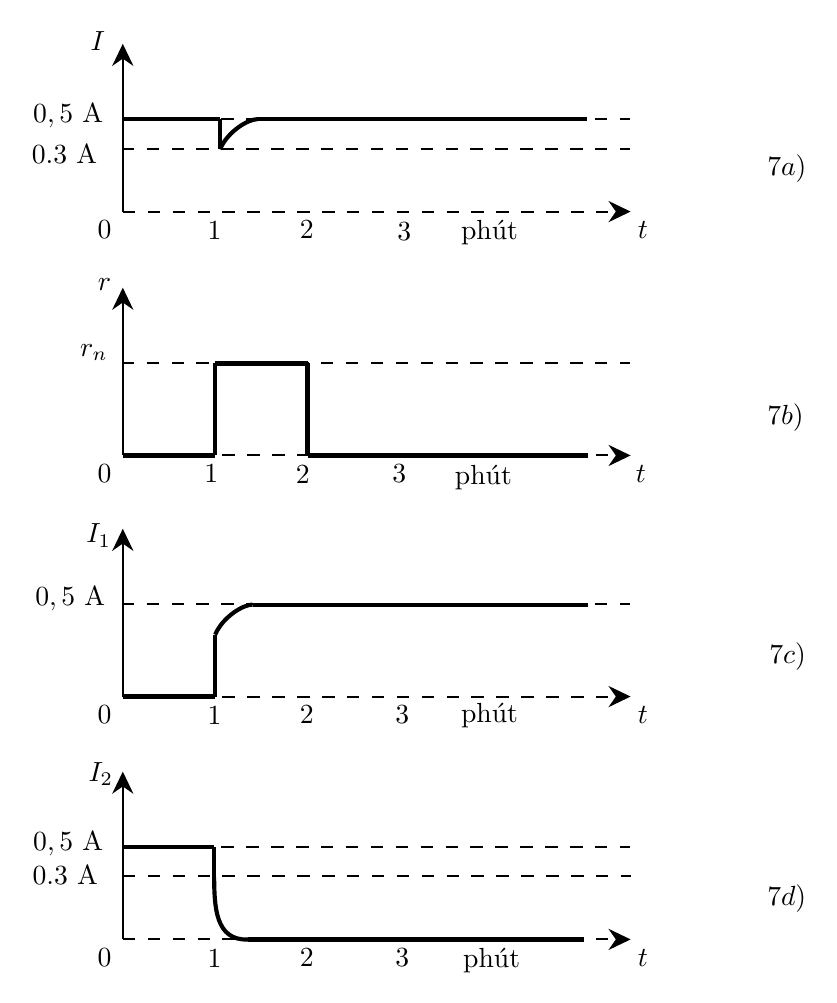
\begin{tikzpicture}[x=0.75pt,y=0.75pt,yscale=-1,xscale=1]
%uncomment if require: \path (0,546); %set diagram left start at 0, and has height of 546

%Straight Lines [id:da3622605915928372] 
\draw    (170,131.5) -- (170,53.67) ;
\draw [shift={(170,50.67)}, rotate = 450] [fill={rgb, 255:red, 0; green, 0; blue, 0 }  ][line width=0.08]  [draw opacity=0] (10.72,-5.15) -- (0,0) -- (10.72,5.15) -- (7.12,0) -- cycle    ;
%Straight Lines [id:da9404061608748968] 
\draw  [dash pattern={on 4.5pt off 4.5pt}]  (170,131.5) -- (411.67,131.5) ;
\draw [shift={(414.67,131.5)}, rotate = 180] [fill={rgb, 255:red, 0; green, 0; blue, 0 }  ][line width=0.08]  [draw opacity=0] (10.72,-5.15) -- (0,0) -- (10.72,5.15) -- (7.12,0) -- cycle    ;
%Straight Lines [id:da707448613408626] 
\draw  [dash pattern={on 4.5pt off 4.5pt}]  (169.5,87) -- (414.17,87) ;
%Straight Lines [id:da874896240588432] 
\draw [line width=1.5]    (169.5,87) -- (216.83,87) ;
%Straight Lines [id:da5672675351855623] 
\draw    (170,249) -- (170,171.17) ;
\draw [shift={(170,168.17)}, rotate = 450] [fill={rgb, 255:red, 0; green, 0; blue, 0 }  ][line width=0.08]  [draw opacity=0] (10.72,-5.15) -- (0,0) -- (10.72,5.15) -- (7.12,0) -- cycle    ;
%Straight Lines [id:da9374137675535845] 
\draw  [dash pattern={on 4.5pt off 4.5pt}]  (170,249) -- (411.67,249) ;
\draw [shift={(414.67,249)}, rotate = 180] [fill={rgb, 255:red, 0; green, 0; blue, 0 }  ][line width=0.08]  [draw opacity=0] (10.72,-5.15) -- (0,0) -- (10.72,5.15) -- (7.12,0) -- cycle    ;
%Straight Lines [id:da2603105587798038] 
\draw  [dash pattern={on 4.5pt off 4.5pt}]  (169.5,204.5) -- (414.17,204.5) ;
%Straight Lines [id:da47141955325658214] 
\draw [line width=1.5]    (259,249) -- (394,249) ;
%Straight Lines [id:da8019199330734006] 
\draw [line width=1.5]    (214.5,204.67) -- (214.5,249) ;
%Straight Lines [id:da031284897541808965] 
\draw [line width=1.5]    (214.5,204.67) -- (259,204.67) ;
%Straight Lines [id:da27012687941849256] 
\draw [line width=1.5]    (259,204.67) -- (259,249) ;
%Straight Lines [id:da8531834591692431] 
\draw [line width=1.5]    (170,249) -- (214.5,249) ;
%Straight Lines [id:da30073485695453495] 
\draw    (170,365.17) -- (170,287.33) ;
\draw [shift={(170,284.33)}, rotate = 450] [fill={rgb, 255:red, 0; green, 0; blue, 0 }  ][line width=0.08]  [draw opacity=0] (10.72,-5.15) -- (0,0) -- (10.72,5.15) -- (7.12,0) -- cycle    ;
%Straight Lines [id:da9515377753441434] 
\draw  [dash pattern={on 4.5pt off 4.5pt}]  (170,365.17) -- (411.67,365.17) ;
\draw [shift={(414.67,365.17)}, rotate = 180] [fill={rgb, 255:red, 0; green, 0; blue, 0 }  ][line width=0.08]  [draw opacity=0] (10.72,-5.15) -- (0,0) -- (10.72,5.15) -- (7.12,0) -- cycle    ;
%Straight Lines [id:da3948231760740648] 
\draw  [dash pattern={on 4.5pt off 4.5pt}]  (169.5,320.67) -- (414.17,320.67) ;
%Straight Lines [id:da02055663791477258] 
\draw    (170,482.17) -- (170,404.33) ;
\draw [shift={(170,401.33)}, rotate = 450] [fill={rgb, 255:red, 0; green, 0; blue, 0 }  ][line width=0.08]  [draw opacity=0] (10.72,-5.15) -- (0,0) -- (10.72,5.15) -- (7.12,0) -- cycle    ;
%Straight Lines [id:da38146925064184756] 
\draw  [dash pattern={on 4.5pt off 4.5pt}]  (170,482.17) -- (411.67,482.17) ;
\draw [shift={(414.67,482.17)}, rotate = 180] [fill={rgb, 255:red, 0; green, 0; blue, 0 }  ][line width=0.08]  [draw opacity=0] (10.72,-5.15) -- (0,0) -- (10.72,5.15) -- (7.12,0) -- cycle    ;
%Straight Lines [id:da31453969533564763] 
\draw  [dash pattern={on 4.5pt off 4.5pt}]  (169.5,437.67) -- (414.17,437.67) ;
%Straight Lines [id:da05018268291352013] 
\draw  [dash pattern={on 4.5pt off 4.5pt}]  (169.5,101.17) -- (414.17,101.17) ;
%Straight Lines [id:da2933139093108008] 
\draw [line width=1.5]    (216.83,101.48) -- (216.83,87) ;
%Straight Lines [id:da15460095282800213] 
\draw [line width=1.5]    (234.83,87) -- (393.8,87) ;
%Curve Lines [id:da6725955731992166] 
\draw [line width=1.5]    (216.83,101.48) .. controls (220.71,92.52) and (230.8,86.9) .. (234.83,87) ;
%Straight Lines [id:da7475796935491477] 
\draw [line width=1.5]    (170,365.17) -- (214.5,365.17) ;
%Straight Lines [id:da4848085287975703] 
\draw [line width=1.5]    (214.5,365.17) -- (214.5,335.33) ;
%Curve Lines [id:da3124656184712311] 
\draw [line width=1.5]    (214.5,335.33) .. controls (218.38,326.38) and (228.47,320.76) .. (232.5,320.86) ;
%Straight Lines [id:da2619787753591578] 
\draw [line width=1.5]    (232.5,320.86) -- (394.2,320.86) ;
%Straight Lines [id:da5919889737937591] 
\draw [line width=1.5]    (169.5,437.67) -- (214,437.67) ;
%Straight Lines [id:da5117932791681985] 
\draw [line width=1.5]    (214,452.14) -- (214,437.67) ;
%Straight Lines [id:da897260510823183] 
\draw [line width=1.5]    (230.5,482.2) -- (392.2,482.2) ;
%Curve Lines [id:da11835083029647753] 
\draw [line width=1.5]    (230.5,482.2) .. controls (214.43,483) and (214.14,466.14) .. (214,452.14) ;
%Straight Lines [id:da8336491239125836] 
\draw  [dash pattern={on 4.5pt off 4.5pt}]  (170,451.67) -- (414.67,451.67) ;

% Text Node
\draw (153,43.4) node [anchor=north west][inner sep=0.75pt]    {$I$};
% Text Node
\draw (416.67,134.9) node [anchor=north west][inner sep=0.75pt]    {$t$};
% Text Node
\draw (125.33,77.9) node [anchor=north west][inner sep=0.75pt]    {$0,5~\mathrm{A}$};
% Text Node
\draw (156.33,134.4) node [anchor=north west][inner sep=0.75pt]    {$0$};
% Text Node
\draw (209.33,134.9) node [anchor=north west][inner sep=0.75pt]    {$1$};
% Text Node
\draw (253.83,134.4) node [anchor=north west][inner sep=0.75pt]    {$2$};
% Text Node
\draw (300.83,135.4) node [anchor=north west][inner sep=0.75pt]    {$3$};
% Text Node
\draw (156.5,162.4) node [anchor=north west][inner sep=0.75pt]    {$r$};
% Text Node
\draw (415.67,252.4) node [anchor=north west][inner sep=0.75pt]    {$t$};
% Text Node
\draw (156.33,251.9) node [anchor=north west][inner sep=0.75pt]    {$0$};
% Text Node
\draw (207.83,251.9) node [anchor=north west][inner sep=0.75pt]    {$1$};
% Text Node
\draw (251.83,252.4) node [anchor=north west][inner sep=0.75pt]    {$2$};
% Text Node
\draw (298.33,251.9) node [anchor=north west][inner sep=0.75pt]    {$3$};
% Text Node
\draw (151,280.57) node [anchor=north west][inner sep=0.75pt]    {$I_{1}$};
% Text Node
\draw (416.67,368.57) node [anchor=north west][inner sep=0.75pt]    {$t$};
% Text Node
\draw (126.33,310.57) node [anchor=north west][inner sep=0.75pt]    {$0,5~\mathrm{A}$};
% Text Node
\draw (156.33,368.07) node [anchor=north west][inner sep=0.75pt]    {$0$};
% Text Node
\draw (209.33,368.57) node [anchor=north west][inner sep=0.75pt]    {$1$};
% Text Node
\draw (253.83,368.07) node [anchor=north west][inner sep=0.75pt]    {$2$};
% Text Node
\draw (299.83,368.07) node [anchor=north west][inner sep=0.75pt]    {$3$};
% Text Node
\draw (152,395.57) node [anchor=north west][inner sep=0.75pt]    {$I_{2}$};
% Text Node
\draw (416.67,485.57) node [anchor=north west][inner sep=0.75pt]    {$t$};
% Text Node
\draw (125.33,428.57) node [anchor=north west][inner sep=0.75pt]    {$0,5~\mathrm{A}$};
% Text Node
\draw (156.33,485.07) node [anchor=north west][inner sep=0.75pt]    {$0$};
% Text Node
\draw (209.33,485.57) node [anchor=north west][inner sep=0.75pt]    {$1$};
% Text Node
\draw (253.83,485.07) node [anchor=north west][inner sep=0.75pt]    {$2$};
% Text Node
\draw (299.83,485.07) node [anchor=north west][inner sep=0.75pt]    {$3$};
% Text Node
\draw (479,102.57) node [anchor=north west][inner sep=0.75pt]    {$7a)$};
% Text Node
\draw (479,222.57) node [anchor=north west][inner sep=0.75pt]    {$7b)$};
% Text Node
\draw (480,337.57) node [anchor=north west][inner sep=0.75pt]    {$7c)$};
% Text Node
\draw (479,454.23) node [anchor=north west][inner sep=0.75pt]    {$7d)$};
% Text Node
\draw (328.5,252) node [anchor=north west][inner sep=0.75pt]   [align=left] {phút};
% Text Node
\draw (331.5,134) node [anchor=north west][inner sep=0.75pt]   [align=left] {phút};
% Text Node
\draw (331.5,367) node [anchor=north west][inner sep=0.75pt]   [align=left] {phút};
% Text Node
\draw (332.5,485) node [anchor=north west][inner sep=0.75pt]   [align=left] {phút};
% Text Node
\draw (148,194.07) node [anchor=north west][inner sep=0.75pt]    {$r_{n}$};
% Text Node
\draw (124.67,97.9) node [anchor=north west][inner sep=0.75pt]    {$0.3~\mathrm{A}$};
% Text Node
\draw (125,444.9) node [anchor=north west][inner sep=0.75pt]    {$0.3~\mathrm{A}$};
\end{tikzpicture}

    \end{center}
    \item Các bước thực hiện là:
    \begin{itemize}
        \item Bước $1$: Đóng công tắc $K$ và tăng dòng điện toàn phần $I$ lên $20~\mathrm{A}$, tức bằng $I_1$. Vì nắt điện đang ở trạng thái $r = 0$ nên $V_M = L\dfrac{\dd I_1}{\dd t} = 0$, nghĩa là $I_1$ không đổi còn $I_2$ tăng thêm $20~\mathrm{A}$, nói cách khác, $I_2$ tăng từ $-20~\mathrm{A}$ đến $0$.
        \item Bước $2$:  Ngắt điện siêu dẫn chuyển từ $0$ đến $r$.
        \item Bước $3$: Giảm dần dòng $I$ về $0$ trong khi giữ $I_2 < 0,5 ~\mathrm{A}$. Vì $I_2 = \dfrac{V_M}{r_n}$ và $V_M = L\dfrac{\dd I_1}{\dd t}$, trong đó $L = 10~\mathrm{H}, r_n = 5~\Omega$. Yêu cầu $I_2 < 0,5~\mathrm{A}$ ứng với $\dfrac{\dd I_1}{\dd t} < 0,25 ~\mathrm{A/s}$ nghĩa là giảm ít hơn $15~\mathrm{A}$ trong $1$ phút. Trên hình $8$ $\dfrac{\dd I}{\dd t} \sim 0,1~\mathrm{A/s}$ và $\dfrac{\dd I_1}{\dd t}$ cũng xấp xỉ giá trị ấy nên yêu cầu được thỏa mãn.
        \item Bước $4$: Chuyển ngắt điện siêu dẫn về giá trị $r = 0$, khi ấy $V_M = 0$ và tắt công tắt $K$. 
    \end{itemize}
    Các kết quả được vẽ trên hình $8$.
    \begin{center}
        

\tikzset{every picture/.style={line width=0.75pt}} %set default line width to 0.75pt        

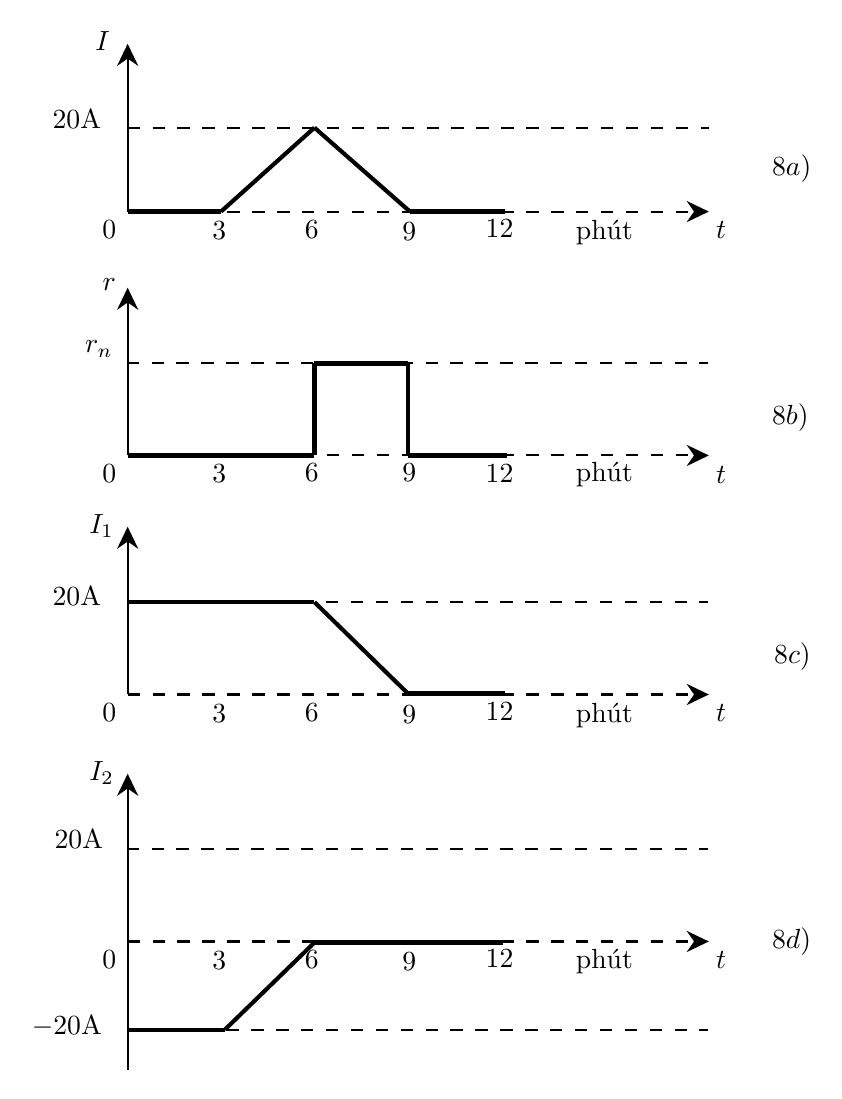
\begin{tikzpicture}[x=0.75pt,y=0.75pt,yscale=-1,xscale=1]
%uncomment if require: \path (0,721); %set diagram left start at 0, and has height of 721

%Straight Lines [id:da9177038101463004] 
\draw  [dash pattern={on 4.5pt off 4.5pt}]  (189.5,319.67) -- (469.5,319.67) ;
%Straight Lines [id:da49737031270433074] 
\draw  [dash pattern={on 4.5pt off 4.5pt}]  (190,249) -- (467,249) ;
\draw [shift={(470,249)}, rotate = 180] [fill={rgb, 255:red, 0; green, 0; blue, 0 }  ][line width=0.08]  [draw opacity=0] (10.72,-5.15) -- (0,0) -- (10.72,5.15) -- (7.12,0) -- cycle    ;
%Straight Lines [id:da0008113661676119044] 
\draw  [dash pattern={on 4.5pt off 4.5pt}]  (189.5,438.67) -- (469.5,438.67) ;
%Straight Lines [id:da481166371070721] 
\draw  [dash pattern={on 4.5pt off 4.5pt}]  (189.5,204.5) -- (469.5,204.5) ;
%Straight Lines [id:da2797124667624027] 
\draw    (190,131.5) -- (190,53.67) ;
\draw [shift={(190,50.67)}, rotate = 450] [fill={rgb, 255:red, 0; green, 0; blue, 0 }  ][line width=0.08]  [draw opacity=0] (10.72,-5.15) -- (0,0) -- (10.72,5.15) -- (7.12,0) -- cycle    ;
%Straight Lines [id:da6648202643395054] 
\draw  [dash pattern={on 4.5pt off 4.5pt}]  (190,131.5) -- (467,131.5) ;
\draw [shift={(470,131.5)}, rotate = 180] [fill={rgb, 255:red, 0; green, 0; blue, 0 }  ][line width=0.08]  [draw opacity=0] (10.72,-5.15) -- (0,0) -- (10.72,5.15) -- (7.12,0) -- cycle    ;
%Straight Lines [id:da582288440655655] 
\draw [line width=1.5]    (190,131.5) -- (235,131.5) ;
%Straight Lines [id:da6492676255712364] 
\draw    (190,249) -- (190,171.17) ;
\draw [shift={(190,168.17)}, rotate = 450] [fill={rgb, 255:red, 0; green, 0; blue, 0 }  ][line width=0.08]  [draw opacity=0] (10.72,-5.15) -- (0,0) -- (10.72,5.15) -- (7.12,0) -- cycle    ;
%Straight Lines [id:da3005030750271125] 
\draw [line width=1.5]    (190,249) -- (280,249) ;
%Straight Lines [id:da6604821210115626] 
\draw    (190,364.17) -- (190,286.33) ;
\draw [shift={(190,283.33)}, rotate = 450] [fill={rgb, 255:red, 0; green, 0; blue, 0 }  ][line width=0.08]  [draw opacity=0] (10.72,-5.15) -- (0,0) -- (10.72,5.15) -- (7.12,0) -- cycle    ;
%Straight Lines [id:da35926289006282297] 
\draw  [dash pattern={on 4.5pt off 4.5pt}]  (190,364.17) -- (467,364.17) ;
\draw [shift={(470,364.17)}, rotate = 180] [fill={rgb, 255:red, 0; green, 0; blue, 0 }  ][line width=0.08]  [draw opacity=0] (10.72,-5.15) -- (0,0) -- (10.72,5.15) -- (7.12,0) -- cycle    ;
%Straight Lines [id:da43753546613122496] 
\draw [line width=1.5]    (189.5,319.67) -- (280,319.67) ;
%Straight Lines [id:da24128318868746002] 
\draw    (190,545) -- (190,405.33) ;
\draw [shift={(190,402.33)}, rotate = 450] [fill={rgb, 255:red, 0; green, 0; blue, 0 }  ][line width=0.08]  [draw opacity=0] (10.72,-5.15) -- (0,0) -- (10.72,5.15) -- (7.12,0) -- cycle    ;
%Straight Lines [id:da09060887757537328] 
\draw  [dash pattern={on 4.5pt off 4.5pt}]  (190,483.17) -- (467,483.17) ;
\draw [shift={(470,483.17)}, rotate = 180] [fill={rgb, 255:red, 0; green, 0; blue, 0 }  ][line width=0.08]  [draw opacity=0] (10.72,-5.15) -- (0,0) -- (10.72,5.15) -- (7.12,0) -- cycle    ;
%Straight Lines [id:da1259269764601494] 
\draw [line width=1.5]    (189.5,525.67) -- (236.83,525.67) ;
%Straight Lines [id:da45912327924945284] 
\draw  [dash pattern={on 4.5pt off 4.5pt}]  (190,91.08) -- (470,91.08) ;
%Straight Lines [id:da33482680228328454] 
\draw  [dash pattern={on 4.5pt off 4.5pt}]  (189.5,525.67) -- (469.5,525.67) ;
%Straight Lines [id:da8903230947994576] 
\draw [line width=1.5]    (235,131.5) -- (280,91.08) ;
%Straight Lines [id:da21421825062842492] 
\draw [line width=1.5]    (280,91.08) -- (326,131.5) ;
%Straight Lines [id:da702497645891849] 
\draw [line width=1.5]    (326,131.5) -- (372,131.5) ;
%Straight Lines [id:da5302587493970403] 
\draw [line width=1.5]    (280,204.67) -- (280,249) ;
%Straight Lines [id:da12348316378735325] 
\draw [line width=1.5]    (280,204.67) -- (325,204.67) ;
%Straight Lines [id:da8733145794724839] 
\draw [line width=1.5]    (325,204.67) -- (325,249) ;
%Straight Lines [id:da04114162853334258] 
\draw [line width=1.5]    (325,249) -- (373,249) ;
%Straight Lines [id:da2787784069118626] 
\draw [line width=1.5]    (325,363.67) -- (372,363.67) ;
%Straight Lines [id:da35165346083235494] 
\draw [line width=1.5]    (280,319.67) -- (325,363.67) ;
%Straight Lines [id:da10786681054271696] 
\draw [line width=1.5]    (236.83,525.67) -- (280,483.67) ;
%Straight Lines [id:da674647620488287] 
\draw [line width=1.5]    (280,483.67) -- (371,483.67) ;

% Text Node
\draw (173,43.4) node [anchor=north west][inner sep=0.75pt]    {$I$};
% Text Node
\draw (472,134.9) node [anchor=north west][inner sep=0.75pt]    {$t$};
% Text Node
\draw (152.33,80.9) node [anchor=north west][inner sep=0.75pt]    {$20\mathrm{A}$};
% Text Node
\draw (176.33,134.4) node [anchor=north west][inner sep=0.75pt]    {$0$};
% Text Node
\draw (229.33,134.9) node [anchor=north west][inner sep=0.75pt]    {$3$};
% Text Node
\draw (273.83,134.4) node [anchor=north west][inner sep=0.75pt]    {$6$};
% Text Node
\draw (320.83,135.4) node [anchor=north west][inner sep=0.75pt]    {$9$};
% Text Node
\draw (176.5,162.4) node [anchor=north west][inner sep=0.75pt]    {$r$};
% Text Node
\draw (176.33,251.9) node [anchor=north west][inner sep=0.75pt]    {$0$};
% Text Node
\draw (499,102.57) node [anchor=north west][inner sep=0.75pt]    {$8a)$};
% Text Node
\draw (499,222.57) node [anchor=north west][inner sep=0.75pt]    {$8b)$};
% Text Node
\draw (500,337.57) node [anchor=north west][inner sep=0.75pt]    {$8c)$};
% Text Node
\draw (499,475.23) node [anchor=north west][inner sep=0.75pt]    {$8d)$};
% Text Node
\draw (404.5,134) node [anchor=north west][inner sep=0.75pt]   [align=left] {phút};
% Text Node
\draw (361,133.73) node [anchor=north west][inner sep=0.75pt]    {$12$};
% Text Node
\draw (472,252.9) node [anchor=north west][inner sep=0.75pt]    {$t$};
% Text Node
\draw (229.33,251.9) node [anchor=north west][inner sep=0.75pt]    {$3$};
% Text Node
\draw (273.83,251.4) node [anchor=north west][inner sep=0.75pt]    {$6$};
% Text Node
\draw (320.83,251.4) node [anchor=north west][inner sep=0.75pt]    {$9$};
% Text Node
\draw (404.5,251) node [anchor=north west][inner sep=0.75pt]   [align=left] {phút};
% Text Node
\draw (361,251.73) node [anchor=north west][inner sep=0.75pt]    {$12$};
% Text Node
\draw (170,276.07) node [anchor=north west][inner sep=0.75pt]    {$I_{1}$};
% Text Node
\draw (472,367.57) node [anchor=north west][inner sep=0.75pt]    {$t$};
% Text Node
\draw (152.33,310.57) node [anchor=north west][inner sep=0.75pt]    {$20\mathrm{A}$};
% Text Node
\draw (176.33,367.07) node [anchor=north west][inner sep=0.75pt]    {$0$};
% Text Node
\draw (229.33,367.57) node [anchor=north west][inner sep=0.75pt]    {$3$};
% Text Node
\draw (273.83,367.07) node [anchor=north west][inner sep=0.75pt]    {$6$};
% Text Node
\draw (320.83,368.07) node [anchor=north west][inner sep=0.75pt]    {$9$};
% Text Node
\draw (404.5,366.67) node [anchor=north west][inner sep=0.75pt]   [align=left] {phút};
% Text Node
\draw (361,366.4) node [anchor=north west][inner sep=0.75pt]    {$12$};
% Text Node
\draw (170,395.07) node [anchor=north west][inner sep=0.75pt]    {$I_{2}$};
% Text Node
\draw (472,486.57) node [anchor=north west][inner sep=0.75pt]    {$t$};
% Text Node
\draw (153.33,427.57) node [anchor=north west][inner sep=0.75pt]    {$20\mathrm{A}$};
% Text Node
\draw (176.33,486.07) node [anchor=north west][inner sep=0.75pt]    {$0$};
% Text Node
\draw (229.33,486.57) node [anchor=north west][inner sep=0.75pt]    {$3$};
% Text Node
\draw (273.83,486.07) node [anchor=north west][inner sep=0.75pt]    {$6$};
% Text Node
\draw (320.83,487.07) node [anchor=north west][inner sep=0.75pt]    {$9$};
% Text Node
\draw (404.5,485.67) node [anchor=north west][inner sep=0.75pt]   [align=left] {phút};
% Text Node
\draw (361,485.4) node [anchor=north west][inner sep=0.75pt]    {$12$};
% Text Node
\draw (142.33,517.57) node [anchor=north west][inner sep=0.75pt]    {$-20\mathrm{A}$};
% Text Node
\draw (168,192.4) node [anchor=north west][inner sep=0.75pt]    {$r_{n}$};
\end{tikzpicture}
    \end{center}
    \item 
    \begin{itemize}
        \item Bước $1$ và bước $2$ cũng giống như trong câu $3$, làm cho dòng $I_2 = 0$.
        \item Bước $3$: Tăng $I$ thêm $10~\mathrm{A}$ để đạt $30~\mathrm{A}$ với tốc độ tăng sao cho thỏa điều kiện $I_2 < 0,5~\mathrm{A}$.
        \item Bước $4$: Chuyển ngắt điện siêu dẫn về trạng thái $r = 0$, khi đó $V_M = 0$.
        \item Bước $5$: Giảm dòng $I$ về $0$, $I_1 = 30~\mathrm{A}$ không đổi vì $V_M = 0$. $I_2 = I - I_1$ sẽ chuyển thành $-30~\mathrm{A}$. Dòng điện qua nam châm bây giờ được đóng mạch do ngắt điện siêu dẫn.
        \item Bước $6$: Mở công tắc $K$. Nam châm bây giờ hoạt động ở chế độ vĩnh cửu.
    \end{itemize}
    Các kết quả được ghi trên hình $9$.
    \begin{center}
        

\tikzset{every picture/.style={line width=0.75pt}} %set default line width to 0.75pt        

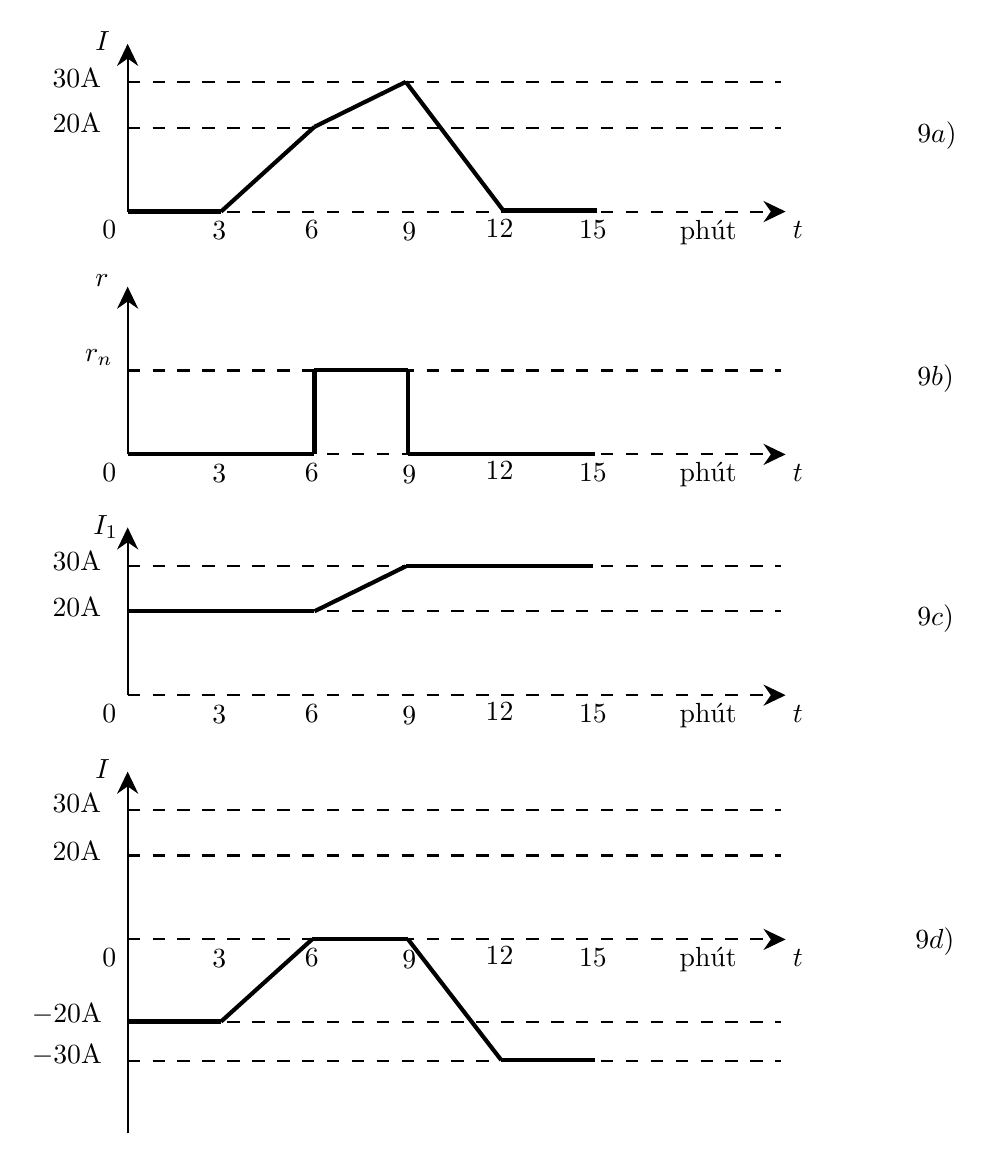
\begin{tikzpicture}[x=0.75pt,y=0.75pt,yscale=-1,xscale=1]
%uncomment if require: \path (0,656); %set diagram left start at 0, and has height of 656

%Straight Lines [id:da4420519557129017] 
\draw  [dash pattern={on 4.5pt off 4.5pt}]  (170,521.75) -- (424,521.75) -- (484.75,521.75) ;
%Straight Lines [id:da49705981879598293] 
\draw    (170,131.5) -- (170,53.67) ;
\draw [shift={(170,50.67)}, rotate = 450] [fill={rgb, 255:red, 0; green, 0; blue, 0 }  ][line width=0.08]  [draw opacity=0] (10.72,-5.15) -- (0,0) -- (10.72,5.15) -- (7.12,0) -- cycle    ;
%Straight Lines [id:da8598925670906716] 
\draw  [dash pattern={on 4.5pt off 4.5pt}]  (170,131.5) -- (484,131.5) ;
\draw [shift={(487,131.5)}, rotate = 180] [fill={rgb, 255:red, 0; green, 0; blue, 0 }  ][line width=0.08]  [draw opacity=0] (10.72,-5.15) -- (0,0) -- (10.72,5.15) -- (7.12,0) -- cycle    ;
%Straight Lines [id:da8231100373261879] 
\draw  [dash pattern={on 4.5pt off 4.5pt}]  (170,91.08) -- (424,91.08) -- (484.75,91.08) ;
%Straight Lines [id:da5941494212249259] 
\draw [line width=1.5]    (170,131.5) -- (215,131.5) ;
%Straight Lines [id:da08895878327051321] 
\draw  [dash pattern={on 4.5pt off 4.5pt}]  (170,69.08) -- (424,69.08) -- (484.75,69.08) ;
%Straight Lines [id:da7578714251862264] 
\draw    (170,248.5) -- (170,170.67) ;
\draw [shift={(170,167.67)}, rotate = 450] [fill={rgb, 255:red, 0; green, 0; blue, 0 }  ][line width=0.08]  [draw opacity=0] (10.72,-5.15) -- (0,0) -- (10.72,5.15) -- (7.12,0) -- cycle    ;
%Straight Lines [id:da44684179436000604] 
\draw  [dash pattern={on 4.5pt off 4.5pt}]  (170,248.5) -- (484,248.5) ;
\draw [shift={(487,248.5)}, rotate = 180] [fill={rgb, 255:red, 0; green, 0; blue, 0 }  ][line width=0.08]  [draw opacity=0] (10.72,-5.15) -- (0,0) -- (10.72,5.15) -- (7.12,0) -- cycle    ;
%Straight Lines [id:da011184537192552524] 
\draw  [dash pattern={on 4.5pt off 4.5pt}]  (170,208.08) -- (424,208.08) -- (484.75,208.08) ;
%Straight Lines [id:da8256331253292983] 
\draw [line width=1.5]    (170,248.5) -- (260,248.5) ;
%Straight Lines [id:da7161566497928653] 
\draw    (170,364.5) -- (170,286.67) ;
\draw [shift={(170,283.67)}, rotate = 450] [fill={rgb, 255:red, 0; green, 0; blue, 0 }  ][line width=0.08]  [draw opacity=0] (10.72,-5.15) -- (0,0) -- (10.72,5.15) -- (7.12,0) -- cycle    ;
%Straight Lines [id:da8258287568515554] 
\draw  [dash pattern={on 4.5pt off 4.5pt}]  (170,364.5) -- (484,364.5) ;
\draw [shift={(487,364.5)}, rotate = 180] [fill={rgb, 255:red, 0; green, 0; blue, 0 }  ][line width=0.08]  [draw opacity=0] (10.72,-5.15) -- (0,0) -- (10.72,5.15) -- (7.12,0) -- cycle    ;
%Straight Lines [id:da940106222677902] 
\draw  [dash pattern={on 4.5pt off 4.5pt}]  (170,324.08) -- (424,324.08) -- (484.75,324.08) ;
%Straight Lines [id:da2809999455580745] 
\draw [line width=1.5]    (170,324.08) -- (260,324.08) ;
%Straight Lines [id:da91713480537205] 
\draw  [dash pattern={on 4.5pt off 4.5pt}]  (170,302.08) -- (424,302.08) -- (484.75,302.08) ;
%Straight Lines [id:da7543277052410247] 
\draw    (170,575.67) -- (170,404.33) ;
\draw [shift={(170,401.33)}, rotate = 450] [fill={rgb, 255:red, 0; green, 0; blue, 0 }  ][line width=0.08]  [draw opacity=0] (10.72,-5.15) -- (0,0) -- (10.72,5.15) -- (7.12,0) -- cycle    ;
%Straight Lines [id:da15298176416220333] 
\draw  [dash pattern={on 4.5pt off 4.5pt}]  (170,482.17) -- (484,482.17) ;
\draw [shift={(487,482.17)}, rotate = 180] [fill={rgb, 255:red, 0; green, 0; blue, 0 }  ][line width=0.08]  [draw opacity=0] (10.72,-5.15) -- (0,0) -- (10.72,5.15) -- (7.12,0) -- cycle    ;
%Straight Lines [id:da9557607260621945] 
\draw  [dash pattern={on 4.5pt off 4.5pt}]  (170,441.75) -- (424,441.75) -- (484.75,441.75) ;
%Straight Lines [id:da7180462350750434] 
\draw [line width=1.5]    (170,521.75) -- (215,521.75) ;
%Straight Lines [id:da3302990309658136] 
\draw  [dash pattern={on 4.5pt off 4.5pt}]  (170,419.75) -- (424,419.75) -- (484.75,419.75) ;
%Straight Lines [id:da9141235126440275] 
\draw  [dash pattern={on 4.5pt off 4.5pt}]  (170,540.75) -- (424,540.75) -- (484.75,540.75) ;
%Straight Lines [id:da009233200512799078] 
\draw [line width=1.5]    (215,131.5) -- (260,90.67) ;
%Straight Lines [id:da30345641200415097] 
\draw [line width=1.5]    (260,90.67) -- (304,69) ;
%Straight Lines [id:da5542701581895288] 
\draw [line width=1.5]    (304,69) -- (351,131) ;
%Straight Lines [id:da41867538342499144] 
\draw [line width=1.5]    (260,248.5) -- (260,207.67) ;
%Straight Lines [id:da9947733120190345] 
\draw [line width=1.5]    (260,207.67) -- (305,207.67) ;
%Straight Lines [id:da5475286076018206] 
\draw [line width=1.5]    (305,248.5) -- (305,207.67) ;
%Straight Lines [id:da06697639264405852] 
\draw [line width=1.5]    (305,248.5) -- (395,248.5) ;
%Straight Lines [id:da49924556554981203] 
\draw [line width=1.5]    (351,131) -- (396,131) ;
%Straight Lines [id:da22560873500685474] 
\draw [line width=1.5]    (260,324.08) -- (304,302.42) ;
%Straight Lines [id:da09180556721252464] 
\draw [line width=1.5]    (304,302.42) -- (394,302.42) ;
%Straight Lines [id:da1124207599610152] 
\draw [line width=1.5]    (259,482) -- (305,482) ;
%Straight Lines [id:da310361333668018] 
\draw [line width=1.5]    (350,540.33) -- (305,482) ;
%Straight Lines [id:da7303638964791419] 
\draw [line width=1.5]    (350,540.33) -- (395,540.33) ;
%Straight Lines [id:da0541943184108884] 
\draw [line width=1.5]    (215,521.75) -- (259,482) ;

% Text Node
\draw (153,43.4) node [anchor=north west][inner sep=0.75pt]    {$I$};
% Text Node
\draw (489,134.9) node [anchor=north west][inner sep=0.75pt]    {$t$};
% Text Node
\draw (132.33,82.9) node [anchor=north west][inner sep=0.75pt]    {$20\mathrm{A}$};
% Text Node
\draw (156.33,134.4) node [anchor=north west][inner sep=0.75pt]    {$0$};
% Text Node
\draw (209.33,134.9) node [anchor=north west][inner sep=0.75pt]    {$3$};
% Text Node
\draw (253.83,134.4) node [anchor=north west][inner sep=0.75pt]    {$6$};
% Text Node
\draw (300.83,135.4) node [anchor=north west][inner sep=0.75pt]    {$9$};
% Text Node
\draw (549,86.57) node [anchor=north west][inner sep=0.75pt]    {$9a)$};
% Text Node
\draw (434.5,134) node [anchor=north west][inner sep=0.75pt]   [align=left] {phút};
% Text Node
\draw (341,133.73) node [anchor=north west][inner sep=0.75pt]    {$12$};
% Text Node
\draw (386,134.4) node [anchor=north west][inner sep=0.75pt]    {$15$};
% Text Node
\draw (132.33,60.9) node [anchor=north west][inner sep=0.75pt]    {$30\mathrm{A}$};
% Text Node
\draw (153,160.4) node [anchor=north west][inner sep=0.75pt]    {$r$};
% Text Node
\draw (489,251.9) node [anchor=north west][inner sep=0.75pt]    {$t$};
% Text Node
\draw (156.33,251.4) node [anchor=north west][inner sep=0.75pt]    {$0$};
% Text Node
\draw (209.33,251.9) node [anchor=north west][inner sep=0.75pt]    {$3$};
% Text Node
\draw (253.83,251.4) node [anchor=north west][inner sep=0.75pt]    {$6$};
% Text Node
\draw (300.83,252.4) node [anchor=north west][inner sep=0.75pt]    {$9$};
% Text Node
\draw (549,203.57) node [anchor=north west][inner sep=0.75pt]    {$9b)$};
% Text Node
\draw (434.5,251) node [anchor=north west][inner sep=0.75pt]   [align=left] {phút};
% Text Node
\draw (341,250.73) node [anchor=north west][inner sep=0.75pt]    {$12$};
% Text Node
\draw (386,251.4) node [anchor=north west][inner sep=0.75pt]    {$15$};
% Text Node
\draw (152,276.4) node [anchor=north west][inner sep=0.75pt]    {$I_{1}$};
% Text Node
\draw (489,367.9) node [anchor=north west][inner sep=0.75pt]    {$t$};
% Text Node
\draw (132.33,315.9) node [anchor=north west][inner sep=0.75pt]    {$20\mathrm{A}$};
% Text Node
\draw (156.33,367.4) node [anchor=north west][inner sep=0.75pt]    {$0$};
% Text Node
\draw (209.33,367.9) node [anchor=north west][inner sep=0.75pt]    {$3$};
% Text Node
\draw (253.83,367.4) node [anchor=north west][inner sep=0.75pt]    {$6$};
% Text Node
\draw (300.83,368.4) node [anchor=north west][inner sep=0.75pt]    {$9$};
% Text Node
\draw (549,319.57) node [anchor=north west][inner sep=0.75pt]    {$9c)$};
% Text Node
\draw (434.5,367) node [anchor=north west][inner sep=0.75pt]   [align=left] {phút};
% Text Node
\draw (341,366.73) node [anchor=north west][inner sep=0.75pt]    {$12$};
% Text Node
\draw (386,367.4) node [anchor=north west][inner sep=0.75pt]    {$15$};
% Text Node
\draw (132.33,293.9) node [anchor=north west][inner sep=0.75pt]    {$30\mathrm{A}$};
% Text Node
\draw (153,394.07) node [anchor=north west][inner sep=0.75pt]    {$I$};
% Text Node
\draw (489,485.57) node [anchor=north west][inner sep=0.75pt]    {$t$};
% Text Node
\draw (132.33,433.57) node [anchor=north west][inner sep=0.75pt]    {$20\mathrm{A}$};
% Text Node
\draw (156.33,485.07) node [anchor=north west][inner sep=0.75pt]    {$0$};
% Text Node
\draw (209.33,485.57) node [anchor=north west][inner sep=0.75pt]    {$3$};
% Text Node
\draw (253.83,485.07) node [anchor=north west][inner sep=0.75pt]    {$6$};
% Text Node
\draw (300.83,486.07) node [anchor=north west][inner sep=0.75pt]    {$9$};
% Text Node
\draw (548,475.23) node [anchor=north west][inner sep=0.75pt]    {$9d)$};
% Text Node
\draw (434.5,484.67) node [anchor=north west][inner sep=0.75pt]   [align=left] {phút};
% Text Node
\draw (341,484.4) node [anchor=north west][inner sep=0.75pt]    {$12$};
% Text Node
\draw (386,485.07) node [anchor=north west][inner sep=0.75pt]    {$15$};
% Text Node
\draw (132.33,410.57) node [anchor=north west][inner sep=0.75pt]    {$30\mathrm{A}$};
% Text Node
\draw (148,196.4) node [anchor=north west][inner sep=0.75pt]    {$r_{n}$};
% Text Node
\draw (122.33,511.57) node [anchor=north west][inner sep=0.75pt]    {$-20\mathrm{A}$};
% Text Node
\draw (122.33,531.57) node [anchor=north west][inner sep=0.75pt]    {$-30\mathrm{A}$};
\end{tikzpicture}
    \end{center}
\end{enumerate}
\end{loigiai}

\begin{vd}[Bật tức thời]
Một máy biến thế gồm một lõi sắt từ hình xuyến (có độ từ hóa $\mu \gg1$) với chiều dài $l< 1 ~\mathrm{m}$ và tiết diện mặt cắt $S$, cuộn sơ cấp có $N_1 = 20$ vòng và cuộn thứ cấp có $N_2 = 100$ vòng. Máy biến thế là một phần của mạch điện được thể hiện trên hình vẽ.
\begin{center}


\tikzset{every picture/.style={line width=0.75pt}} %set default line width to 0.75pt        

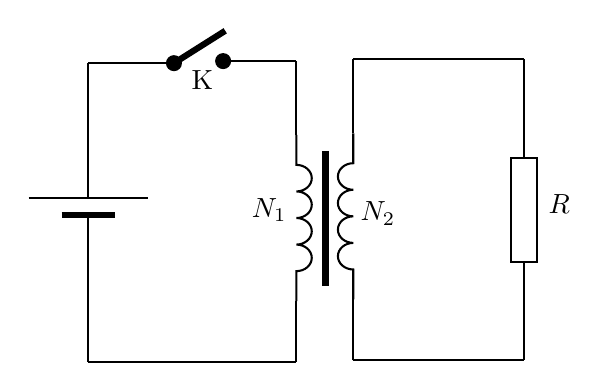
\begin{tikzpicture}[x=0.75pt,y=0.75pt,yscale=-1,xscale=1]
%uncomment if require: \path (0,300); %set diagram left start at 0, and has height of 300

%Straight Lines [id:da6897041654057285] 
\draw    (203.7,213.8) -- (304,213.8) ;
%Straight Lines [id:da13203459476295043] 
\draw    (203.7,213.8) -- (203.7,142.8) ;
%Straight Lines [id:da6385637755262643] 
\draw    (304,213.8) -- (304,184.4) ;
%Straight Lines [id:da20048328577729957] 
\draw    (331.4,103.6) -- (331.4,68) ;
%Straight Lines [id:da6188967294774059] 
\draw    (304,68.8) -- (268.7,68.8) ;
\draw [shift={(268.7,68.8)}, rotate = 180] [color={rgb, 255:red, 0; green, 0; blue, 0 }  ][fill={rgb, 255:red, 0; green, 0; blue, 0 }  ][line width=0.75]      (0, 0) circle [x radius= 3.35, y radius= 3.35]   ;
%Straight Lines [id:da9480852333785736] 
\draw    (245,69.8) -- (203.7,69.8) ;
\draw [shift={(245,69.8)}, rotate = 180] [color={rgb, 255:red, 0; green, 0; blue, 0 }  ][fill={rgb, 255:red, 0; green, 0; blue, 0 }  ][line width=0.75]      (0, 0) circle [x radius= 3.35, y radius= 3.35]   ;
%Straight Lines [id:da9895905934104963] 
\draw    (203.7,134.8) -- (203.7,69.8) ;
%Shape: Inductor (Air Core) [id:dp9252111777802665] 
\draw   (304,104.4) -- (304,118.8) .. controls (308.08,118.8) and (311.4,121.67) .. (311.4,125.2) .. controls (311.4,128.73) and (308.08,131.6) .. (304,131.6) .. controls (308.08,131.6) and (311.4,134.47) .. (311.4,138) .. controls (311.4,141.53) and (308.08,144.4) .. (304,144.4) .. controls (308.08,144.4) and (311.4,147.27) .. (311.4,150.8) .. controls (311.4,154.33) and (308.08,157.2) .. (304,157.2) .. controls (308.08,157.2) and (311.4,160.07) .. (311.4,163.6) .. controls (311.4,167.13) and (308.08,170) .. (304,170) -- (304,184.4) ;
%Straight Lines [id:da2454204779869844] 
\draw    (331.4,213) -- (413.7,213) ;
%Straight Lines [id:da041147928920516996] 
\draw    (331.4,213) -- (331.4,183.6) ;
%Straight Lines [id:da7960273025439635] 
\draw    (304,104.4) -- (304,68.8) ;
%Shape: Inductor (Air Core) [id:dp6838018215732404] 
\draw   (331.4,183.6) -- (331.4,169.2) .. controls (327.32,169.2) and (324,166.33) .. (324,162.8) .. controls (324,159.27) and (327.32,156.4) .. (331.4,156.4) .. controls (327.32,156.4) and (324,153.53) .. (324,150) .. controls (324,146.47) and (327.32,143.6) .. (331.4,143.6) .. controls (327.32,143.6) and (324,140.73) .. (324,137.2) .. controls (324,133.67) and (327.32,130.8) .. (331.4,130.8) .. controls (327.32,130.8) and (324,127.93) .. (324,124.4) .. controls (324,120.87) and (327.32,118) .. (331.4,118) -- (331.4,103.6) ;
%Straight Lines [id:da6972269819681767] 
\draw    (331.4,68) -- (413.7,68) ;
%Straight Lines [id:da3356019596591966] 
\draw    (413.7,213) -- (413.7,68) ;
%Straight Lines [id:da19382391406082378] 
\draw [line width=2.25]    (318,112) -- (318,177.2) ;
%Shape: Rectangle [id:dp5402243054566243] 
\draw  [fill={rgb, 255:red, 255; green, 255; blue, 255 }  ,fill opacity=1 ] (407.35,115.4) -- (420.05,115.4) -- (420.05,165.6) -- (407.35,165.6) -- cycle ;
%Straight Lines [id:da9137907411136375] 
\draw [line width=2.25]    (245,69.8) -- (269.7,54.2) ;
%Straight Lines [id:da6575373168861844] 
\draw [line width=2.25]    (190.85,142.8) -- (216.55,142.8) ;
%Straight Lines [id:da8905291120826924] 
\draw    (175.03,134.8) -- (232.38,134.8) ;


% Text Node
\draw (252,72) node [anchor=north west][inner sep=0.75pt]   [align=left] {K};
% Text Node
\draw (281,133.4) node [anchor=north west][inner sep=0.75pt]    {$N_{1}$};
% Text Node
\draw (333.4,135.2) node [anchor=north west][inner sep=0.75pt]    {$N_{2}$};
% Text Node
\draw (424,131.4) node [anchor=north west][inner sep=0.75pt]    {$R$};


\end{tikzpicture}
\end{center}

Suất điện động của nguồn là $\varepsilon = 24~\mathrm{V}$, điện trở trong của nguồn là $r= 4~ \Omega.$ Cuộn dây thứ cấp được kết nối với một điện trở $R= 100~ \Omega$. Ban đầu khi khóa $K$ mở, không có dòng điện chạy trong mạch. Sau đó khóa $K$ được đóng đột ngột. Điện trở của khóa chạy về không vô cùng nhanh (nhưng không phải tức thời) trong khoảng thời gian rất nhỏ hơn $\tau \equiv \dfrac{\mu_0 \mu N_1^2 S}{lr}= 0,05$ giây. Điện trở của hai cuộn dây là vô cùng nhỏ. Sự mất mát từ thông khi truyền giữa hai cuộn dây là không đáng kể.
\begin{enumerate}[1)]
\item Dẫn ra một phương trình liên hệ giữa từ thông $\phi$ trong lõi và các dòng điện $I_1$ và $I_2$ trong các cuộn dây sơ cấp và thứ cấp. Xem rằng chiều dòng điện dương của hai cuộn dây là như nhau.
\item Xét mạch kín bao gồm cuộn dây sơ cấp và điện trở trong của nguồn điện. Coi rằng trong thời gian khóa $K$ đóng, hiệu điện thế hai đầu mạch biến thiên theo quy luật $U_1 = U(t)$. Viết hệ phương trình chứa đạo hàm bậc nhất của $I_1(t)$ và $I_2(t)$ mô tả dòng điện trong cuộn sơ cấp và thứ cấp.
\item Xác định giá trị ban đầu của $I_1(0)$ và $I_2(0)$ (điều kiện biên của các phương trình vi phân ở câu trên).
\item Xác định tỉ lệ của dòng điện trong cuộn dây thứ cấp ở thời điểm $t_1 = 2\tau$ và thời điểm $t_2 = 4\tau$ sau khi nguồn điện $U(t)$ được bật lên. Đưa ra một giá trị tính số gần đúng của tỉ số $\dfrac{I_2(2\tau)}{I_2 (4\tau)}$.
\item Xác định giá trị của dòng điện cực đại trong cuộn dây thứ cấp sau khi mạch điện được đóng. Đưa ra biểu thức cho $I_{2}^{\max}$ theo các thông số đề bài cho và tính giá trị số gần đúng cho $I_{2}^{\max}$.
\item Tìm biểu thức dòng điện phụ thuộc thời gian $I_2(t)$ ở thời điểm $t>\tau$ theo các thông số đề bài.
\item Vẽ một đồ thị gần đúng cho sự phụ thuộc $I_2(t)$ từ thời điểm công tắc được đóng cho đến $T= 0,5$ giây.
\item Tính dòng điện cực đại ở cuộn dây sơ cấp sau khi công tắc được đóng. Dẫn ra biểu thức của $I_{1}^{\max}$ theo các thông số đề bài và tính giá trị số.
\item Tìm biểu thức phụ thuộc $I_1(t)$ cho $t>\tau$ theo các thông số đề bài.
\item Vẽ đồ thị gần đúng của sự phụ thuộc $I_1(t)$ từ thời điểm công tắc được đóng cho đến khi $T= 0,5$ giây.
\end{enumerate}
\end{vd}


\begin{loigiai}
\begin{enumerate}[1)]
\item Vì chiều dài của lõi $l<1~\mathrm{m}$ có thể coi là đạt điều kiện chuẩn dừng nên mối liên hệ giữa từ thông trong lõi và dòng điện chạy trong hai cuộn dây có mối liên hệ:
   $$
\Phi=\dfrac{\mu_{0} \mu S}{l}\left[N_{1} I_{1}+N_{2} I_{2}\right],
$$
(chọn cùng chiều dòng điện dương cho hai cuộn dây).
\item Nếu hiệu điện thế của hai đầu mạch sơ cấp sau khi đóng khóa $K$ biến thiên theo quy luật $U_1 = U(t)$, định luật Kirchhoff sẽ cho ta (nếu bỏ qua điện trở của cuộn dây):
\[\heva{U(t)-N_{1} \dfrac{\mu_{0} \mu S}{l}\left[N_{1} \dfrac{\dd I_{1}}{\dd t}+N_{2} \dfrac{\dd I_{2}}{\dd t}\right] &= I_{1} r, \\
-N_{2} \dfrac{\mu_{0} \mu S}{l}\left[N_{1} \dfrac{\dd I_{1}}{d t}+N_{2} \dfrac{\dd I_{2}}{\dd t}\right] &= I_{2} R.}\]

\item Vì dòng điện trong cuộn dây không thể thay đổi một cách đột ngột, điều kiện đầu tại $t=0$ (thời điểm đóng khóa $K$) phải đạt được là $I_1(0)=I_2(0)=0$.
\item Bằng cách nhân phương trình đầu với $N_1$ và phương trình sau với $N_2$ và sau đó thế hai phương trình ta thu được: 
   $$
I_{1}=\dfrac{U(t)}{r}+\dfrac{R}{k r} I_{2},
$$
ở mọi thời điểm (ở đây $k \equiv \dfrac{N_1}{N_2}$). Thế phương trình này vào phương trình thứ hai ta thu được phương trình dòng điện ở cuộn dây thứ cấp:
    $$\dfrac{\dd I_{2}}{\dd t}+\dfrac{R}{R+k^{2} r} \cdot \dfrac{I_{2}}{\tau}=-\dfrac{k}{R+k^{2} r} \dfrac{\dd U}{\dd t}.$$
Do đó, ngay khi hiệu điện thế hai đầu mạch sơ cấp bằng giá trị của suất điện động pin và trở nên gần như không đổi ($\dfrac{\dd U}{\dd t} \approx 0$), sự phụ thuộc $I_2(t)$ sẽ được tính gần đúng là:
    $$I_{2}(t) \approx C \cdot \exp \left[-\dfrac{R}{\left(R+k^{2} r\right) \tau} t\right]=C \cdot \exp \left[-\dfrac{t}{2 \tau}\right].$$
Ta thay số vào phương trình trên theo các giá trị $R$, $r$ và $k$. Từ đây ta thu được:
   $$
\dfrac{I_{2}(2 \tau)}{I_{2}(4 \tau)} \approx e \approx 2.72.$$
\item Tuy nhiên phương trình trên không thể xác định trực tiếp biểu thức cuối cho $I_2(t)$ vì hằng số $C \neq 0$ phải được tính là dòng điện ở cuối quá trình ``bật tức thời'' của nguồn điện. Để làm được điều này, ta phải xây dựng một hàm $U(t)$ sao cho $U(0)=0$ và $U(\tau_0) = \varepsilon$, ở đây $\tau_0 \ll \tau $ là thời gian bật của pin (thời gian để điện trở của điểm nối giảm về không). Ví dụ, chúng ta xét $U(t) \approx \varepsilon \dfrac{t}{\tau_0}$ trong khoảng thời gian từ không tới $\tau_0$. Do đó, đối với $t \leq \tau_0$ chúng ta thu được:
   $$\dfrac{\dd I_{2}}{\dd t}+\dfrac{R}{R+k^{2} r} \cdot \dfrac{I_{2}}{\tau} \approx-\dfrac{k}{R+k^{2} r} \cdot \dfrac{\varepsilon}{\tau_{0}} \Rightarrow \dfrac{\dd I_{2}}{\dd t} \approx-\dfrac{k}{R+k^{2} r} \cdot \dfrac{\varepsilon}{\tau_{0}},$$
(thành phần chứa $I_2$ có thể được bỏ qua do $I_2 \leq k \dfrac{\varepsilon}{R}$ và $\dfrac{\tau_0}{\tau} \ll 1$), ở đây $I_2(0) =0$. Do đó, trong khoảng thời gian này ta có:
   $$I_{2}(t) \approx-\dfrac{k}{R+k^{2} r} \cdot \dfrac{\varepsilon}{\tau_{0}} t.$$
Điều này thể hiện rằng ở cuối của quá trình ``bật tức thời'', dòng điện ở cuộn dây thứ cấp ngược chiều với dòng điện ở cuộn dây sơ cấp.
\item Dòng điện cực đại trong cuộn dây thứ cấp là:
    $$
I_{2}^{\max } \approx \dfrac{k \varepsilon}{R+k^{2} r} \approx 0.6 \mathrm{~A}.
$$
Sau đó, dòng điện suy giảm theo hàm
   $$
I_{2}(t) \approx-\dfrac{k \varepsilon}{R+k^{2} r} \cdot \exp \left[-\dfrac{R}{\left(R+k^{2} r\right) \tau} t\right].
$$
\item Vì $\dfrac{RT}{(R_k^2 r)\tau} =5 $, dòng điện ở cuộn dây sơ cấp ở $T=0,5$ giây sẽ nhỏ hơn $0,7\% $ so với giá trị cực đại. Do đó, một đồ thị gần đúng cho $I_2(t)$ được thể hiện ở hình vẽ dưới.
  \begin{center}


\tikzset{every picture/.style={line width=0.75pt}} %set default line width to 0.75pt        

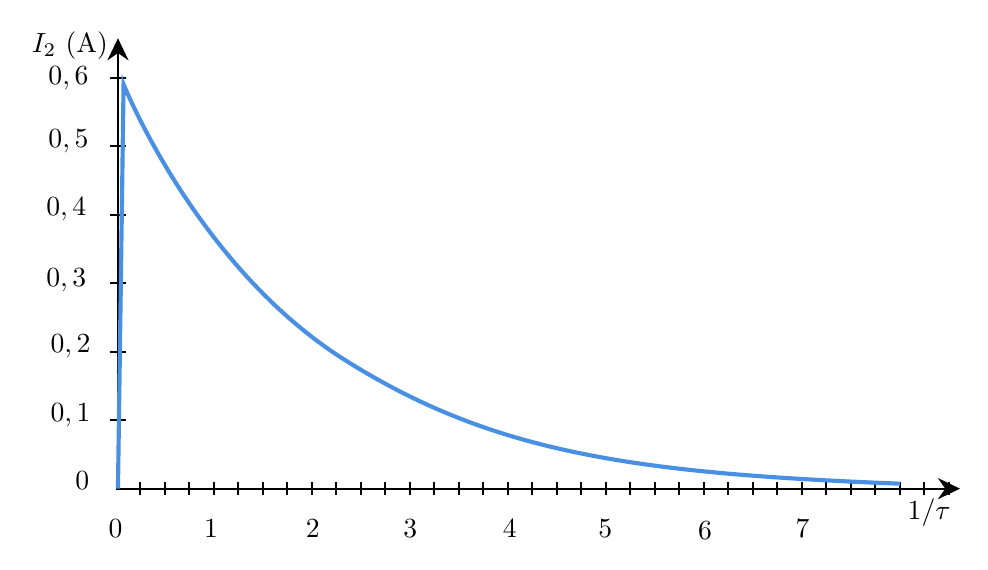
\begin{tikzpicture}[x=0.75pt,y=0.75pt,yscale=-1,xscale=1]
%uncomment if require: \path (0,393); %set diagram left start at 0, and has height of 393

%Straight Lines [id:da855065133258567] 
\draw    (166,263) -- (569.7,263) (177.8,260) -- (177.8,266)(189.6,260) -- (189.6,266)(201.4,260) -- (201.4,266)(213.2,260) -- (213.2,266)(225,260) -- (225,266)(236.8,260) -- (236.8,266)(248.6,260) -- (248.6,266)(260.4,260) -- (260.4,266)(272.2,260) -- (272.2,266)(284,260) -- (284,266)(295.8,260) -- (295.8,266)(307.6,260) -- (307.6,266)(319.4,260) -- (319.4,266)(331.2,260) -- (331.2,266)(343,260) -- (343,266)(354.8,260) -- (354.8,266)(366.6,260) -- (366.6,266)(378.4,260) -- (378.4,266)(390.2,260) -- (390.2,266)(402,260) -- (402,266)(413.8,260) -- (413.8,266)(425.6,260) -- (425.6,266)(437.4,260) -- (437.4,266)(449.2,260) -- (449.2,266)(461,260) -- (461,266)(472.8,260) -- (472.8,266)(484.6,260) -- (484.6,266)(496.4,260) -- (496.4,266)(508.2,260) -- (508.2,266)(520,260) -- (520,266)(531.8,260) -- (531.8,266)(543.6,260) -- (543.6,266)(555.4,260) -- (555.4,266)(567.2,260) -- (567.2,266) ;
\draw [shift={(572.7,263)}, rotate = 180] [fill={rgb, 255:red, 0; green, 0; blue, 0 }  ][line width=0.08]  [draw opacity=0] (10.72,-5.15) -- (0,0) -- (10.72,5.15) -- (7.12,0) -- cycle    ;
%Straight Lines [id:da8764626731237466] 
\draw    (167,263) -- (167,49) (163,230) -- (171,230)(163,197) -- (171,197)(163,164) -- (171,164)(163,131) -- (171,131)(163,98) -- (171,98)(163,65) -- (171,65) ;
\draw [shift={(167,46)}, rotate = 450] [fill={rgb, 255:red, 0; green, 0; blue, 0 }  ][line width=0.08]  [draw opacity=0] (10.72,-5.15) -- (0,0) -- (10.72,5.15) -- (7.12,0) -- cycle    ;
%Curve Lines [id:da08280362912197425] 
\draw [color={rgb, 255:red, 74; green, 144; blue, 226 }  ,draw opacity=1 ][line width=1.5]    (167,263) .. controls (168.7,142.6) and (169.7,68.2) .. (169.7,68.2) .. controls (169.7,68.2) and (204.7,155.6) .. (275.7,200.6) .. controls (346.7,245.6) and (414.7,255.6) .. (543.7,260.6) ;


% Text Node
\draw (161,276.4) node [anchor=north west][inner sep=0.75pt]    {$0$};
% Text Node
\draw (207,276.4) node [anchor=north west][inner sep=0.75pt]    {$1$};
% Text Node
\draw (256,276.4) node [anchor=north west][inner sep=0.75pt]    {$2$};
% Text Node
\draw (303,276.4) node [anchor=north west][inner sep=0.75pt]    {$3$};
% Text Node
\draw (351,276.4) node [anchor=north west][inner sep=0.75pt]    {$4$};
% Text Node
\draw (397,276.4) node [anchor=north west][inner sep=0.75pt]    {$5$};
% Text Node
\draw (445,277.4) node [anchor=north west][inner sep=0.75pt]    {$6$};
% Text Node
\draw (492,276.4) node [anchor=north west][inner sep=0.75pt]    {$7$};
% Text Node
\draw (546,266.4) node [anchor=north west][inner sep=0.75pt]    {$1/\tau $};
% Text Node
\draw (145,253.4) node [anchor=north west][inner sep=0.75pt]    {$0$};
% Text Node
\draw (133,220.4) node [anchor=north west][inner sep=0.75pt]    {$0,1$};
% Text Node
\draw (133,187.4) node [anchor=north west][inner sep=0.75pt]    {$0,2$};
% Text Node
\draw (131,155.4) node [anchor=north west][inner sep=0.75pt]    {$0,3$};
% Text Node
\draw (131,121.4) node [anchor=north west][inner sep=0.75pt]    {$0,4$};
% Text Node
\draw (132,88.4) node [anchor=north west][inner sep=0.75pt]    {$0,5$};
% Text Node
\draw (132,58.4) node [anchor=north west][inner sep=0.75pt]    {$0,6$};
% Text Node
\draw (124,41.4) node [anchor=north west][inner sep=0.75pt]    {$I_{2}~(\mathrm{A})$};


\end{tikzpicture}
\end{center}
\item 9) 10) Sử dụng các phương trình đã thu được ở trên chúng ta tìm được biểu thức cho dòng điện chạy trong cuộn sơ cấp:
  \[I_{1}(t) \approx\left\{\begin{array}{cc}
  \dfrac{k^{2}}{R+k^{2} r} \dfrac{\varepsilon}{\tau_{0}} t, & t \leq \tau_{0} ; \\
  \dfrac{\varepsilon}{r}\left[1-\dfrac{R}{R+k^{2} r} \exp \left(-\dfrac{R}{\left(R+k^{2} r\right) \tau} t\right)\right], & t>\tau_{0}.\end{array}\right.\]
Do đó, ngay sau khi quá trình đóng mạch bắt đầu, dòng điện ở cuộn dây thứ cấp rất nhanh (với $\tau_0 \ll \tau$) tăng đến giá trị $\dfrac{k^2 \varepsilon}{R + k^2 r} \approx 3~\mathrm{A}$ và sau đó chậm rãi tiến đến giá trị ổn định $\dfrac{\varepsilon}{r} =6 ~\mathrm{A}$ và xấp xỉ đạt được giá trị đó tại thời điểm $T$. Một đồ thị gần đúng của $I_1(t)$ được thể hiện trên hình vẽ.
  \begin{center}
 
 
\tikzset{every picture/.style={line width=0.75pt}} %set default line width to 0.75pt        
 
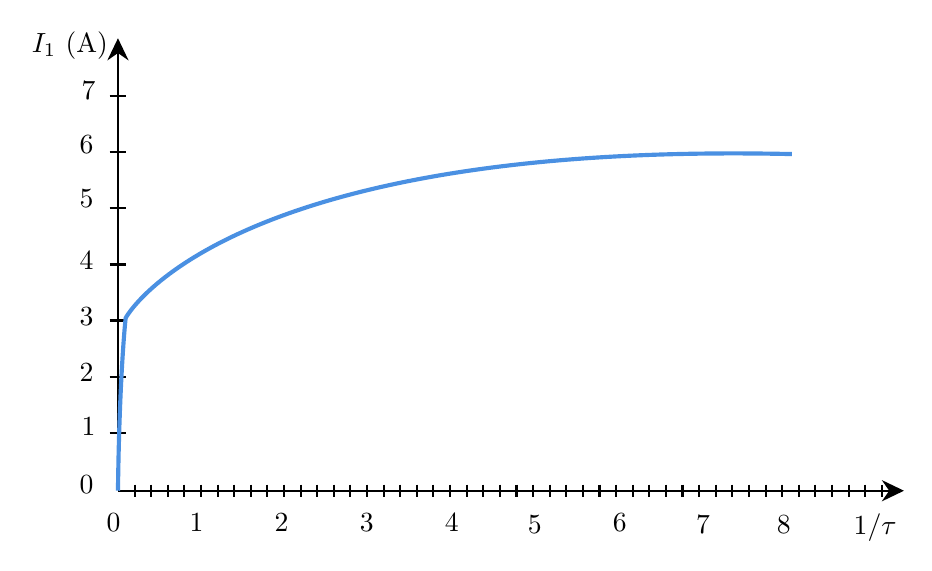
\begin{tikzpicture}[x=0.75pt,y=0.75pt,yscale=-1,xscale=1]
%uncomment if require: \path (0,291); %set diagram left start at 0, and has height of 291
 
%Straight Lines [id:da8247638492749725] 
\draw    (172,247) -- (547.7,247) (180,244) -- (180,250)(188,244) -- (188,250)(196,244) -- (196,250)(204,244) -- (204,250)(212,244) -- (212,250)(220,244) -- (220,250)(228,244) -- (228,250)(236,244) -- (236,250)(244,244) -- (244,250)(252,244) -- (252,250)(260,244) -- (260,250)(268,244) -- (268,250)(276,244) -- (276,250)(284,244) -- (284,250)(292,244) -- (292,250)(300,244) -- (300,250)(308,244) -- (308,250)(316,244) -- (316,250)(324,244) -- (324,250)(332,244) -- (332,250)(340,244) -- (340,250)(348,244) -- (348,250)(356,244) -- (356,250)(364,244) -- (364,250)(372,244) -- (372,250)(380,244) -- (380,250)(388,244) -- (388,250)(396,244) -- (396,250)(404,244) -- (404,250)(412,244) -- (412,250)(420,244) -- (420,250)(428,244) -- (428,250)(436,244) -- (436,250)(444,244) -- (444,250)(452,244) -- (452,250)(460,244) -- (460,250)(468,244) -- (468,250)(476,244) -- (476,250)(484,244) -- (484,250)(492,244) -- (492,250)(500,244) -- (500,250)(508,244) -- (508,250)(516,244) -- (516,250)(524,244) -- (524,250)(532,244) -- (532,250)(540,244) -- (540,250) ;
\draw [shift={(550.7,247)}, rotate = 180] [fill={rgb, 255:red, 0; green, 0; blue, 0 }  ][line width=0.08]  [draw opacity=0] (10.72,-5.15) -- (0,0) -- (10.72,5.15) -- (7.12,0) -- cycle    ;
%Straight Lines [id:da72713247435419] 
\draw    (172,246) -- (172,32) (168,219) -- (176,219)(168,192) -- (176,192)(168,165) -- (176,165)(168,138) -- (176,138)(168,111) -- (176,111)(168,84) -- (176,84)(168,57) -- (176,57) ;
\draw [shift={(172,29)}, rotate = 450] [fill={rgb, 255:red, 0; green, 0; blue, 0 }  ][line width=0.08]  [draw opacity=0] (10.72,-5.15) -- (0,0) -- (10.72,5.15) -- (7.12,0) -- cycle    ;
%Curve Lines [id:da7704435517389567] 
\draw [color={rgb, 255:red, 74; green, 144; blue, 226 }  ,draw opacity=1 ][line width=1.5]    (172,247) .. controls (172.7,190.8) and (175.7,163.8) .. (175.7,163.8) .. controls (175.7,163.8) and (220.7,78.6) .. (496.7,84.8) ;
 
% Text Node
\draw (165,256.4) node [anchor=north west][inner sep=0.75pt]    {$0$};
% Text Node
\draw (205,256.4) node [anchor=north west][inner sep=0.75pt]    {$1$};
% Text Node
\draw (246,256.4) node [anchor=north west][inner sep=0.75pt]    {$2$};
% Text Node
\draw (287,256.4) node [anchor=north west][inner sep=0.75pt]    {$3$};
% Text Node
\draw (328,256.4) node [anchor=north west][inner sep=0.75pt]    {$4$};
% Text Node
\draw (368,257.4) node [anchor=north west][inner sep=0.75pt]    {$5$};
% Text Node
\draw (409,256.4) node [anchor=north west][inner sep=0.75pt]    {$6$};
% Text Node
\draw (449,257.4) node [anchor=north west][inner sep=0.75pt]    {$7$};
% Text Node
\draw (488,257.4) node [anchor=north west][inner sep=0.75pt]    {$8$};
% Text Node
\draw (525,256.4) node [anchor=north west][inner sep=0.75pt]    {$1/\tau $};
% Text Node
\draw (152,238.4) node [anchor=north west][inner sep=0.75pt]    {$0$};
% Text Node
\draw (153,210.4) node [anchor=north west][inner sep=0.75pt]    {$1$};
% Text Node
\draw (152,184.4) node [anchor=north west][inner sep=0.75pt]    {$2$};
% Text Node
\draw (152,157.4) node [anchor=north west][inner sep=0.75pt]    {$3$};
% Text Node
\draw (152,130.4) node [anchor=north west][inner sep=0.75pt]    {$4$};
% Text Node
\draw (152,100.4) node [anchor=north west][inner sep=0.75pt]    {$5$};
% Text Node
\draw (152,74.4) node [anchor=north west][inner sep=0.75pt]    {$6$};
% Text Node
\draw (153,48.4) node [anchor=north west][inner sep=0.75pt]    {$7$};
% Text Node
\draw (129,24.4) node [anchor=north west][inner sep=0.75pt]    {$I_{1}~(\mathrm{A})$};
 
 
\end{tikzpicture}
\end{center}
Chú ý rằng dòng điện cực đại trong cuộn dây sơ cấp sau khi mạch đóng (kết quả của câu $8)$) có thể được tính đơn giản bằng cách xét trường hợp dòng điện ở hai cuộn dây là hằng số và suất điện động cảm ứng ở trong hai cuộn dây bằng không.\\
\textbf{Lưu ý:} Dĩ nhiên rằng mô hình tuyến tính cho $U(t)$ trong khoảng thời gian ``bật tức thời'' là không bắt buộc, mọi mô hình hợp lí đều cho ra kết quả gần tương tự nhau trong khoảng $\tau_0 \ll \tau$. Mô hình tuyến tính chỉ là mô hình đơn giản nhất. Ví dụ, chúng ta có thể định nghĩa
     $$U(t) \approx \varepsilon \dfrac{t}{\tau_{0}}\left(2-\dfrac{t}{\tau_{0}}\right),$$
cho $t \leq \tau_0$ (một biểu thức cong trơn ở điểm chuyển tiếp $U(t) \approx \varepsilon$ với $t\leq \tau_0$). Một cách làm hiệu quả khác đó chính là chọn biểu thức
    $$U(t)= \varepsilon \cdot\left[1-e^{ \left(-t / \tau_{0}\right)}\right],$$
(mô tả này là đúng với mọi $t$, do đó chúng ta không cần dùng hai hàm cho hai quãng thời gian khác nhau). Do đó, chúng ta sẽ phải giải một phương trình vi phân phức tạp hơn và thu được lời giải:
\[\begin{aligned}
    I_{2}(t) &= \dfrac{k \varepsilon}{R+k^{2} r} \cdot\left[\exp \left(-\dfrac{t}{\tau_{0}}\right)-\exp \left(-\dfrac{R t}{\left(R+k^{2} r\right) \tau}\right)\right],\\
    I_{1}(t) &\approx \dfrac{\varepsilon}{r} \cdot\left[1-\dfrac{k^{2} r}{R+k^{2} r} \exp \left(-\dfrac{t}{\tau_{0}}\right)-\dfrac{R}{R+k^{2} r} \exp \left(-\dfrac{R t}{\left(R+k^{2} r\right) \tau}\right)\right].
\end{aligned}\]
   
Chúng ta có thể thấy, với mọi mô hình, sự phụ thuộc của dòng điện vào thời gian trong khoảng $\tau_0\ll \tau$ là như nhau (do đó $I_{2}^{\max} $ cũng là như nhau) tương tự với mô hình tuyến tính. 
\end{enumerate}
\end{loigiai}

\begin{vd}[Mạch khuếch đại pin]\\
    Để có nguồn điện có hiệu điện thế cao bằng pin, người ta dùng đoạn mạch sau.
    \\Một công tắc điện từ $K_1$ nối một pin có suất điện động $E$ với cuộn cảm có độ tự cảm $L$: nó đóng nếu trong cuộn cảm không có dòng điện (lò xo giữ nó đóng), nhưng nếu dòng điện trong cuộn cảm đạt giá trị tới hạn $I_0$ thì từ trường được tạo bởi cuộn cảm sẽ kéo nó mở. Do quán tính, một khi khóa đã mở, cần một khoảng thời gian nhất định $\tau_K$ để đóng lại ngay cả khi dòng điện giảm về không.
    \\Đối với diode $D$, bạn có thể giả định rằng dòng điện của nó bằng không đối với bất kỳ điện áp ngược nào $(V_D <0)$ và đối với bất kỳ điện áp thuận nào nhỏ hơn điện áp mở $V_0$ (tức là cho $0 <V_D <V_0)$. Đối với bất kỳ dòng điện thuận nào khác không, điện áp của diode $V_D$ đều bằng $V_0$.
    \\Bạn có thể biểu diễn các kết quả theo $L,~E,~I_0,~V_0$ và điện dung $C$ (xem hình vẽ).
    \begin{center}
        

\tikzset{every picture/.style={line width=0.75pt}} %set default line width to 0.75pt        

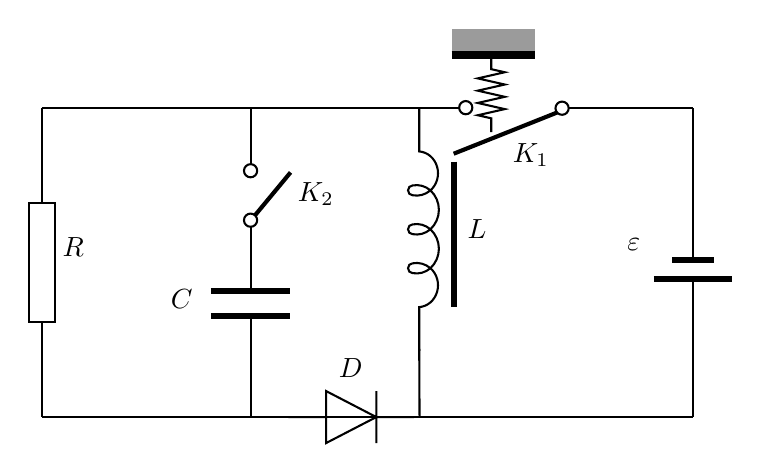
\begin{tikzpicture}[x=0.75pt,y=0.75pt,yscale=-1,xscale=1]
%uncomment if require: \path (0,521); %set diagram left start at 0, and has height of 521

%Straight Lines [id:da11142939000156349] 
\draw    (97.45,120) -- (97.45,269.08) ;
%Straight Lines [id:da11356844905882446] 
\draw    (97.45,120) -- (298.44,120) ;
%Straight Lines [id:da12494577393228479] 
\draw    (351.2,120.26) -- (410.94,120.26) ;
%Straight Lines [id:da6549789482998163] 
\draw    (410.94,120.26) -- (410.94,193.51) ;
%Straight Lines [id:da7908024127293314] 
\draw    (410.94,202.6) -- (410.94,269.08) ;
%Straight Lines [id:da126927769569803] 
\draw    (97.45,269.08) -- (410.94,269.08) ;
%Straight Lines [id:da1562269692992182] 
\draw    (197.94,120) -- (197.94,147.22) ;
%Straight Lines [id:da07076026015682313] 
\draw    (197.94,177.4) -- (197.94,208.51) ;
%Straight Lines [id:da6608265176343087] 
\draw [line width=2.25]    (178.79,208.51) -- (217.09,208.51) ;
%Straight Lines [id:da01869770884462585] 
\draw [line width=2.25]    (178.79,220.4) -- (217.09,220.4) ;
%Straight Lines [id:da08124205152605946] 
\draw    (197.94,220.4) -- (197.94,269.08) ;
%Shape: Diode [id:dp1758927390953775] 
\draw   (234.33,256.55) -- (258.51,269.08) -- (234.33,281.6) -- (234.33,256.55) -- cycle (216.2,269.08) -- (234.33,269.08) (258.51,256.55) -- (258.51,281.6) (258.51,269.08) -- (276.64,269.08) ;
%Shape: Inductor (Air Core) [id:dp14572860138547017] 
\draw   (279.2,120) -- (279.2,141.1) .. controls (283.2,141.4) and (286.61,144.33) .. (287.8,148.47) .. controls (289,152.62) and (287.73,157.13) .. (284.6,159.85) .. controls (282.17,161.94) and (279.02,162.8) .. (275.96,162.19) .. controls (274.77,162.19) and (273.8,161.14) .. (273.8,159.85) .. controls (273.8,158.55) and (274.77,157.5) .. (275.96,157.5) .. controls (279.02,156.9) and (282.17,157.75) .. (284.6,159.85) .. controls (287.2,162.28) and (288.67,165.68) .. (288.67,169.22) .. controls (288.67,172.77) and (287.2,176.16) .. (284.6,178.6) .. controls (282.17,180.69) and (279.02,181.55) .. (275.96,180.94) .. controls (274.77,180.94) and (273.8,179.89) .. (273.8,178.6) .. controls (273.8,177.31) and (274.77,176.26) .. (275.96,176.26) .. controls (279.02,175.65) and (282.17,176.51) .. (284.6,178.6) .. controls (287.2,181.04) and (288.67,184.43) .. (288.67,187.98) .. controls (288.67,191.52) and (287.2,194.92) .. (284.6,197.35) .. controls (282.17,199.45) and (279.02,200.3) .. (275.96,199.7) .. controls (274.77,199.7) and (273.8,198.65) .. (273.8,197.35) .. controls (273.8,196.06) and (274.77,195.01) .. (275.96,195.01) .. controls (279.02,194.4) and (282.17,195.26) .. (284.6,197.35) .. controls (287.73,200.07) and (289,204.58) .. (287.8,208.73) .. controls (286.61,212.87) and (283.2,215.8) .. (279.2,216.1) -- (279.2,237.2) ;
%Straight Lines [id:da7026494423224043] 
\draw    (279.2,236.2) -- (279.35,269.02) ;
%Straight Lines [id:da009555528342141129] 
\draw [line width=2.25]    (401.2,193.51) -- (421.2,193.51) ;
%Straight Lines [id:da6868847749521525] 
\draw [line width=2.25]    (392.2,202.6) -- (430.09,202.6) ;
%Shape: Circle [id:dp9039655080115059] 
\draw   (194.76,174.22) .. controls (194.76,172.47) and (196.19,171.04) .. (197.94,171.04) .. controls (199.7,171.04) and (201.12,172.47) .. (201.12,174.22) .. controls (201.12,175.98) and (199.7,177.4) .. (197.94,177.4) .. controls (196.19,177.4) and (194.76,175.98) .. (194.76,174.22) -- cycle ;
%Shape: Circle [id:dp539652557394968] 
\draw   (194.76,150.39) .. controls (194.76,148.64) and (196.19,147.22) .. (197.94,147.22) .. controls (199.7,147.22) and (201.12,148.64) .. (201.12,150.39) .. controls (201.12,152.15) and (199.7,153.57) .. (197.94,153.57) .. controls (196.19,153.57) and (194.76,152.15) .. (194.76,150.39) -- cycle ;
%Shape: Circle [id:dp5595402579980537] 
\draw   (298.44,120) .. controls (298.44,118.24) and (299.86,116.82) .. (301.62,116.82) .. controls (303.37,116.82) and (304.79,118.24) .. (304.79,120) .. controls (304.79,121.76) and (303.37,123.18) .. (301.62,123.18) .. controls (299.86,123.18) and (298.44,121.76) .. (298.44,120) -- cycle ;
%Shape: Circle [id:dp2923688067821817] 
\draw   (344.84,120.26) .. controls (344.84,118.51) and (346.27,117.08) .. (348.02,117.08) .. controls (349.78,117.08) and (351.2,118.51) .. (351.2,120.26) .. controls (351.2,122.02) and (349.78,123.44) .. (348.02,123.44) .. controls (346.27,123.44) and (344.84,122.02) .. (344.84,120.26) -- cycle ;
%Shape: Rectangle [id:dp7157880602665709] 
\draw  [draw opacity=0][fill={rgb, 255:red, 155; green, 155; blue, 155 }  ,fill opacity=1 ] (294.8,81.97) -- (334.8,81.97) -- (334.8,94.8) -- (294.8,94.8) -- cycle ;
%Straight Lines [id:da7280968760637461] 
\draw [line width=3]    (294.8,94.8) -- (334.8,94.8) ;
%Shape: Resistor [id:dp22063949198262733] 
\draw   (313.9,94.8) -- (313.9,101.46) -- (320.4,102.94) -- (307.4,105.9) -- (320.4,108.86) -- (307.4,111.82) -- (320.4,114.78) -- (307.4,117.74) -- (320.4,120.7) -- (307.4,123.66) -- (313.9,125.14) -- (313.9,131.8) ;
%Straight Lines [id:da9694535109174542] 
\draw [line width=1.5]    (345.84,122.26) -- (295.8,142.2) ;
%Straight Lines [id:da7350531204026427] 
\draw [line width=1.5]    (217.2,151.2) -- (199.94,172.04) ;
%Straight Lines [id:da735776063217783] 
\draw [line width=2.25]    (296,146) -- (296,216.2) ;
%Shape: Rectangle [id:dp8198792718253196] 
\draw  [fill={rgb, 255:red, 255; green, 255; blue, 255 }  ,fill opacity=1 ] (91.05,165.94) -- (103.85,165.94) -- (103.85,223.14) -- (91.05,223.14) -- cycle ;


% Text Node
\draw (158,206.4) node [anchor=north west][inner sep=0.75pt]    {$C$};
% Text Node
\draw (239,239.4) node [anchor=north west][inner sep=0.75pt]    {$D$};
% Text Node
\draw (301,172.4) node [anchor=north west][inner sep=0.75pt]    {$L$};
% Text Node
\draw (219.2,154.6) node [anchor=north west][inner sep=0.75pt]    {$K_{2}$};
% Text Node
\draw (322.82,135.63) node [anchor=north west][inner sep=0.75pt]    {$K_{1}$};
% Text Node
\draw (105.85,181.34) node [anchor=north west][inner sep=0.75pt]    {$R$};
% Text Node
\draw (378,181.4) node [anchor=north west][inner sep=0.75pt]  {$\varepsilon $};


\end{tikzpicture}
    \end{center}
    \begin{enumerate}[1)]
        \item Đầu tiên mở khóa $K_2$. Nếu dòng điện qua cuộn cảm ban đầu bằng không thì sau khoảng thời gian $
        \tau_L$ bằng bao nhiêu thì khóa $K_1$ mở?
        \item  Giả sử (cho cả phần sau) rằng $L/R \ll \tau_K \ll \tau_L$, hãy vẽ đồ thị dòng điện dẫn dưới dạng hàm của thời gian 
        $t$ (với $0 \leqslant t < 3\tau_L$).
        \item Hiệu điện thế cực đại $V_\mathrm{max}$ trên biến trở $R$ là?
        \item Giả sử $V_\mathrm{max}$ là $V_0$ thì công suất tiêu hao trung bình trên diode là bao nhiêu?
    \end{enumerate}
\end{vd}
\begin{loigiai}\[\]
    \begin{enumerate}[1)]
        \item Áp dụng định luật Kirchoff cho vòng mạch gồm $L$ và $\varepsilon$, ta có:
        \[\varepsilon=L \dfrac{\mathrm{d}I}{\mathrm{d}t},\]
        do đó:
        \[I=\dfrac{\varepsilon t}{L}.\]
        Mặt khác, $I_0=\dfrac{\varepsilon \tau_L}{L}$ nên:
        \[\tau_L=\dfrac{LI_0}{\varepsilon}.\]
        \item Khi dòng điện đạt đến $I_0$, khóa sẽ được mở, dòng điện qua $L$ không thể thay đổi ngay lập tức và buộc phải tắt dần thông qua điện trở R. Vì thời gian đặc trưng của dòng điện này (bao gồm $L$ và $R$ là rất ngắn $(L/R \ll \tau_K)$), dòng điện giảm rất nhanh và về không trong khi khóa vẫn mở. Bây giờ không có dòng điện qua cuộn cảm để khóa sẽ đóng lại và quá trình sẽ bắt đầu lặp lại từ đầu. Kết quả là chúng ta sẽ có đồ thị tuần hoàn như hình:
        \begin{center}
            \tikzset{every picture/.style={line width=0.75pt}} %set default line width to 0.75pt        
            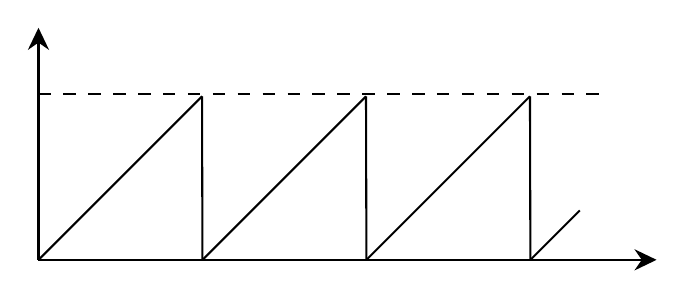
\begin{tikzpicture}[x=0.75pt,y=0.75pt,yscale=-1,xscale=1]
            \draw    (163,195) -- (163,86.2) ;
            \draw [shift={(163,83.2)}, rotate = 450] [fill={rgb, 255:red, 0; green, 0; blue, 0 }  ][line width=0.08]  [draw opacity=0] (10.72,-5.15) -- (0,0) -- (10.72,5.15) -- (7.12,0) -- cycle    ;
            \draw    (163,195) -- (457.8,195) ;
            \draw [shift={(460.8,195)}, rotate = 180] [fill={rgb, 255:red, 0; green, 0; blue, 0 }  ][line width=0.08]  [draw opacity=0] (10.72,-5.15) -- (0,0) -- (10.72,5.15) -- (7.12,0) -- cycle    ;
            \draw  [dash pattern={on 4.5pt off 4.5pt}]  (163,115) -- (433.8,115) ;
            \draw    (163,195) -- (241.8,116.2) ;
            \draw    (242,195) -- (320.8,116.2) ;
            \draw    (321,195) -- (399.8,116.2) ;
            \draw    (242,195) -- (241.8,116.2) ;
            \draw    (321,195) -- (320.8,116.2) ;
            \draw    (400,195) -- (399.8,116.2) ;
            \draw    (400,195) -- (423.8,171.2) ;
        \end{tikzpicture}
        \end{center}
        \item Điện áp qua điện trở cực đại khi cường độ dòng điện cực đại, điều này xảy ra ngay sau khi mở công tắc; dòng điện cực đại là $I_0$ nên:
        \[V_\mathrm{max} = RI_0.\]
        \item Vì $V_\mathrm{max} \gg V_0$, ta có thể bỏ qua ảnh hưởng của diode. Từ định luật Kirchoff, ta có:
        \[L\dfrac{\mathrm{d}I}{\mathrm{d}t}=RI=R\dfrac{\mathrm{d}q}{\mathrm{d}t}.\]
        Lấy tích phân trong một chu kỳ (khi dòng điện giảm từ $I_0$ tới 0), ta được:
        \[LI_0=R \Delta q,\]
        do đó điện tích qua điện trở (và diode) là \[\Delta q=\dfrac{I_0 L}{R}.\] Trong suốt chu kỳ, diode có hiệu điện thế không đổi là $V_0$ nên điện trường thực hiện công:
        \[A=V_0 \Delta q\]
        tỏa ra dưới dạng nhiệt trong diode. Vì vậy công suất tiêu thụ trung bình là:
        \[P=\dfrac{A}{\tau_L}=\dfrac{V_0 I_0 L}{R \tau_L}=\dfrac{V_0 \varepsilon}{R}.\]
    \end{enumerate}
\end{loigiai}


\begin{vd}[Dynamo tự kích điện]
Một đĩa kim loại có bán kính $a$, gắn vào một trục mảnh, quay với tốc độ góc không đổi $\omega$ trong lòng một ống dây thẳng, có chiều dài $l$, có độ tự cảm $L$; hai đầu cuộn dây được mắc thành mạch điện với đĩa quay nhờ hai chổi quét như trên hình. Điện trở toàn phần của cả mạch là $R$. Một sự nhiễu loạn từ trường nhỏ có thể khơi mào cho một suất điện động cảm ứng tăng dần giữa hai đầu $P$, $Q$.
\begin{enumerate}[1)]
    \item Hãy viết phương trình vi phân cho dòng điện $i(t)$ chạy trong mạch. Viết kết quả theo $L$, $R$ và suất điện động cảm ứng $\mathcal{E}$ giữa hai đầu $P$ và $Q$.
    \item  Hãy xác định cảm ứng từ $(B)$ theo $i, N, l$, và $\mu_{0}$. Bỏ qua từ trường gây nên bởi đĩa và trục quay. 
    \item Hãy tìm biểu thức của suất điện động cảm ứng $(\mathcal{E})$ theo $\mu_{0}, N, a, l, i$ và tốc độ góc $\omega$.    
    \item Giải phương trình ở câu $1)$ cho giá trị dòng điện ở một thời điểm bất kì $t$ theo giá trị dòng điện ở thời điểm ban đầu $i(0)$ và các tham số khác.
    \item Hãy cho biết giá trị tối thiểu của tốc độ góc để cho dòng điện mạnh lên dần. Viết kết quả theo $R, \mu_{0}, N, a$, và $l$.
\begin{center}
\tikzset{every picture/.style={line width=0.75pt}} %set default line width to 0.75pt        

\begin{tikzpicture}[x=0.75pt,y=0.75pt,yscale=-0.65,xscale=0.65,scale=0.7]
%uncomment if require: \path (0,725); %set diagram left start at 0, and has height of 725

%Shape: Can [id:dp7604484302816266] 
\draw  [fill={rgb, 255:red, 255; green, 255; blue, 255 }  ,fill opacity=1 ] (265.7,534.5) -- (265.79,299.25) .. controls (265.79,298.56) and (267.64,298.01) .. (269.93,298.01) .. controls (272.21,298.01) and (274.07,298.57) .. (274.07,299.25) -- (273.99,534.5) .. controls (273.99,535.19) and (272.13,535.74) .. (269.84,535.74) .. controls (267.56,535.74) and (265.7,535.18) .. (265.7,534.5) .. controls (265.7,533.81) and (267.56,533.25) .. (269.85,533.26) .. controls (272.13,533.26) and (273.99,533.81) .. (273.99,534.5) ;
%Shape: Ellipse [id:dp9073150731380437] 
\draw  [fill={rgb, 255:red, 255; green, 255; blue, 255 }  ,fill opacity=1 ] (223.99,298.18) .. controls (224.03,289.06) and (243.96,281.75) .. (268.51,281.84) .. controls (293.06,281.94) and (312.93,289.41) .. (312.89,298.52) .. controls (312.86,307.64) and (292.93,314.96) .. (268.38,314.86) .. controls (243.83,314.77) and (223.96,307.3) .. (223.99,298.18) -- cycle ;
%Shape: Ellipse [id:dp7831632242132669] 
\draw  [fill={rgb, 255:red, 255; green, 255; blue, 255 }  ,fill opacity=1 ] (224.02,289.93) .. controls (224.06,280.81) and (243.99,273.49) .. (268.54,273.59) .. controls (293.09,273.68) and (312.96,281.15) .. (312.93,290.27) .. controls (312.89,299.39) and (292.96,306.7) .. (268.41,306.61) .. controls (243.86,306.51) and (223.99,299.05) .. (224.02,289.93) -- cycle ;
%Straight Lines [id:da15211630183630298] 
\draw [fill={rgb, 255:red, 255; green, 255; blue, 255 }  ,fill opacity=1 ]   (224.03,288.68) -- (223.99,298.18) ;
%Straight Lines [id:da4152297399713436] 
\draw    (312.93,290.27) -- (312.89,298.52) ;

%Shape: Can [id:dp5127794527972624] 
\draw  [fill={rgb, 255:red, 255; green, 255; blue, 255 }  ,fill opacity=1 ] (273.35,29.99) -- (274,298) .. controls (274,298) and (272.18,298) .. (269.93,298.01) .. controls (267.68,298.02) and (265.85,298.02) .. (265.85,298.02) -- (265.2,30.01) .. controls (265.2,30.01) and (267.02,30.01) .. (269.27,30) .. controls (271.52,30) and (273.35,29.99) .. (273.35,29.99) .. controls (273.35,29.99) and (271.52,30) .. (269.27,30) .. controls (267.02,30.01) and (265.2,30.01) .. (265.2,30.01) ;
%Shape: Spring [id:dp7488865465602574] 
\draw   (271.18,484.01) .. controls (233.02,481.1) and (194.86,473.57) .. (194.86,458.54) .. controls (194.87,428.47) and (347.53,428.52) .. (347.53,435.46) .. controls (347.53,442.4) and (194.87,442.34) .. (194.88,412.27) .. controls (194.89,382.2) and (347.55,382.26) .. (347.54,389.2) .. controls (347.54,396.13) and (194.88,396.08) .. (194.89,366.01) .. controls (194.9,335.94) and (347.56,335.99) .. (347.56,342.93) .. controls (347.56,349.87) and (194.9,349.82) .. (194.91,319.75) .. controls (194.92,289.68) and (347.58,289.73) .. (347.58,296.67) .. controls (347.57,303.61) and (194.92,303.56) .. (194.93,273.48) .. controls (194.94,243.41) and (347.59,243.47) .. (347.59,250.41) .. controls (347.59,257.35) and (194.93,257.29) .. (194.94,227.22) .. controls (194.95,197.15) and (347.61,197.2) .. (347.61,204.14) .. controls (347.61,211.08) and (194.95,211.03) .. (194.96,180.96) .. controls (194.97,150.89) and (347.63,150.94) .. (347.62,157.88) .. controls (347.62,164.82) and (194.96,164.77) .. (194.97,134.69) .. controls (194.98,104.62) and (347.64,104.68) .. (347.64,111.62) .. controls (347.64,118.56) and (194.98,118.5) .. (194.99,88.43) .. controls (195,58.36) and (347.66,58.41) .. (347.66,65.35) .. controls (347.66,70.33) and (269.18,71.71) .. (224.77,61.01) ;
%Straight Lines [id:da5630346149293071] 
\draw    (424.69,483.06) -- (269.83,483.01) ;
%Straight Lines [id:da47499195768076596] 
\draw    (424.69,521) -- (274,521) ;
\draw [shift={(271,521)}, rotate = 360] [fill={rgb, 255:red, 0; green, 0; blue, 0 }  ][line width=0.08]  [draw opacity=0] (10.72,-5.15) -- (0,0) -- (10.72,5.15) -- (7.12,0) -- cycle    ;
%Straight Lines [id:da8696990269799538] 
\draw    (424.69,521) -- (424.69,483.06) ;
\draw [shift={(424.69,521)}, rotate = 270] [color={rgb, 255:red, 0; green, 0; blue, 0 }  ][fill={rgb, 255:red, 0; green, 0; blue, 0 }  ][line width=0.75]      (0, 0) circle [x radius= 3.35, y radius= 3.35]   ;
%Shape: Arc [id:dp47701387251480987] 
\draw  [draw opacity=0] (265.15,24.36) .. controls (266.18,24.27) and (267.25,24.23) .. (268.33,24.23) .. controls (278.64,24.23) and (287,28.21) .. (287,33.12) .. controls (286.99,38.02) and (278.64,42) .. (268.33,41.99) .. controls (258.02,41.99) and (249.67,38.01) .. (249.67,33.11) .. controls (249.67,30.45) and (252.13,28.06) .. (256.02,26.43) -- (268.33,33.11) -- cycle ; \draw   (265.15,24.36) .. controls (266.18,24.27) and (267.25,24.23) .. (268.33,24.23) .. controls (278.64,24.23) and (287,28.21) .. (287,33.12) .. controls (286.99,38.02) and (278.64,42) .. (268.33,41.99) .. controls (258.02,41.99) and (249.67,38.01) .. (249.67,33.11) .. controls (249.67,30.45) and (252.13,28.06) .. (256.02,26.43) ;
\draw   (276.01,28.65) .. controls (271.55,26.19) and (267.23,24.85) .. (263.06,24.62) .. controls (267.1,23.73) and (271.01,21.72) .. (274.78,18.58) ;

%Straight Lines [id:da733838350163033] 
\draw    (270,62) -- (416,62) ;
%Straight Lines [id:da6775431897128024] 
\draw    (416,62) -- (416,149) ;
%Shape: Resistor [id:dp6779924473844934] 
\draw   (416,149) -- (415.99,162.86) -- (435.24,165.96) -- (396.73,172.09) -- (435.24,178.28) -- (396.72,184.42) -- (435.23,190.61) -- (396.71,196.74) -- (435.22,202.93) -- (396.7,209.07) -- (415.96,212.16) -- (415.95,226.03) ;
%Straight Lines [id:da6026431717982224] 
\draw    (415.95,226.03) -- (415.95,311.02) ;
\draw [shift={(415.95,311.02)}, rotate = 90] [color={rgb, 255:red, 0; green, 0; blue, 0 }  ][fill={rgb, 255:red, 0; green, 0; blue, 0 }  ][line width=0.75]      (0, 0) circle [x radius= 3.35, y radius= 3.35]   ;
%Straight Lines [id:da26180785748529756] 
\draw    (298.13,311.02) -- (415.95,311.02) ;
\draw [shift={(295.13,311.02)}, rotate = 0] [fill={rgb, 255:red, 0; green, 0; blue, 0 }  ][line width=0.08]  [draw opacity=0] (10.72,-5.15) -- (0,0) -- (10.72,5.15) -- (7.12,0) -- cycle    ;
%Straight Lines [id:da4991351312278298] 
\draw    (268.47,290.1) -- (243.77,276.94) ;
\draw [shift={(242,276)}, rotate = 388.03999999999996] [color={rgb, 255:red, 0; green, 0; blue, 0 }  ][line width=0.75]    (10.93,-3.29) .. controls (6.95,-1.4) and (3.31,-0.3) .. (0,0) .. controls (3.31,0.3) and (6.95,1.4) .. (10.93,3.29)   ;
%Straight Lines [id:da7968373327917957] 
\draw    (189,536) -- (265.13,506.72) ;
\draw [shift={(267,506)}, rotate = 518.96] [color={rgb, 255:red, 0; green, 0; blue, 0 }  ][line width=0.75]    (10.93,-3.29) .. controls (6.95,-1.4) and (3.31,-0.3) .. (0,0) .. controls (3.31,0.3) and (6.95,1.4) .. (10.93,3.29)   ;
%Straight Lines [id:da22059494271578495] 
\draw    (394,372) -- (345.76,345.95) ;
\draw [shift={(344,345)}, rotate = 388.37] [color={rgb, 255:red, 0; green, 0; blue, 0 }  ][line width=0.75]    (10.93,-3.29) .. controls (6.95,-1.4) and (3.31,-0.3) .. (0,0) .. controls (3.31,0.3) and (6.95,1.4) .. (10.93,3.29)   ;

% Text Node
\draw (244,279.4) node [anchor=north west][inner sep=0.75pt]    {$a$};
% Text Node
\draw (419,307.4) node [anchor=north west][inner sep=0.75pt]    {$P$};
% Text Node
\draw (432,513.4) node [anchor=north west][inner sep=0.75pt]    {$Q$};
% Text Node
\draw (286,9.4) node [anchor=north west][inner sep=0.75pt]    {$\omega $};
% Text Node
\draw (145,537) node [anchor=north west][inner sep=0.75pt]   [align=left] {Chổi quét};
% Text Node
\draw (364.5,369.5) node [anchor=north west][inner sep=0.75pt]   [align=left] {Solenoid };

\end{tikzpicture}
\end{center}
\item Để giữ giá trị tốc độ góc $\omega$ không đổi, cần phải tác dụng vào trục quay một moment lực bằng bao nhiêu ở thời điểm $t$?
\end{enumerate}
\end{vd}

\begin{loigiai}\[\]
\begin{enumerate}[1)]
\item Phương trình vi phân đối với $i(t)$ theo $L$, $R$ và $\mathcal{E}$:
\[L \dfrac{\dd i}{\dd t}+R i=\mathcal{E}. \tag{1} \label{1z}\]
\item Nếu chiều dài $l$ của solenoid lớn hơn nhiều so với đường kính của nó thì mật độ từ thông qua tiết diện của solenoid được cho bởi:
\[B=\dfrac{\mu_{0} N i}{l}. \tag{2}\]
\item Tìm biểu thức của $\mathcal{E}$ theo $\mu_0$, $a$, $l$, $i$ và $\omega$.
\begin{center}
\tikzset{every picture/.style={line width=0.75pt}} %set default line width to 0.75pt
\begin{tikzpicture}[x=0.75pt,y=0.75pt,yscale=-1,xscale=1]
%uncomment if require: \path (0,300); %set diagram left start at 0, and has height of 300
%Shape: Circle [id:dp6982145546368537] 
\draw   (114,134) .. controls (114,93.13) and (147.13,60) .. (188,60) .. controls (228.87,60) and (262,93.13) .. (262,134) .. controls (262,174.87) and (228.87,208) .. (188,208) .. controls (147.13,208) and (114,174.87) .. (114,134) -- cycle ;
%Straight Lines [id:da21799845372928073] 
\draw    (188,134) -- (335.62,134) ;
\draw [shift={(335.62,134)}, rotate = 0] [color={rgb, 255:red, 0; green, 0; blue, 0 }  ][fill={rgb, 255:red, 0; green, 0; blue, 0 }  ][line width=0.75]      (0, 0) circle [x radius= 3.35, y radius= 3.35]   ;
\draw [shift={(261.81,134)}, rotate = 0] [fill={rgb, 255:red, 0; green, 0; blue, 0 }  ][line width=0.08]  [draw opacity=0] (10.72,-5.15) -- (0,0) -- (10.72,5.15) -- (7.12,0) -- cycle    ;
\draw [shift={(188,134)}, rotate = 0] [color={rgb, 255:red, 0; green, 0; blue, 0 }  ][fill={rgb, 255:red, 0; green, 0; blue, 0 }  ][line width=0.75]      (0, 0) circle [x radius= 3.35, y radius= 3.35]   ;
%Straight Lines [id:da8989346078920936] 
\draw    (219,134) -- (219,102) ;
\draw [shift={(219,99)}, rotate = 450] [fill={rgb, 255:red, 0; green, 0; blue, 0 }  ][line width=0.08]  [draw opacity=0] (10.72,-5.15) -- (0,0) -- (10.72,5.15) -- (7.12,0) -- cycle    ;
%Straight Lines [id:da44122871908464045] 
\draw  [dash pattern={on 4.5pt off 4.5pt}]  (188,134) -- (123.03,169) ;
%Shape: Arc [id:dp6237544388117521] 
\draw  [draw opacity=0] (175.88,135.31) .. controls (175.82,134.88) and (175.8,134.44) .. (175.8,134) .. controls (175.8,127.58) and (181.26,122.38) .. (188,122.38) .. controls (194.74,122.38) and (200.2,127.58) .. (200.2,134) .. controls (200.2,137.05) and (198.97,139.83) .. (196.95,141.9) -- (188,134) -- cycle ; \draw   (175.88,135.31) .. controls (175.82,134.88) and (175.8,134.44) .. (175.8,134) .. controls (175.8,127.58) and (181.26,122.38) .. (188,122.38) .. controls (194.74,122.38) and (200.2,127.58) .. (200.2,134) .. controls (200.2,137.05) and (198.97,139.83) .. (196.95,141.9) ;
\draw   (179.33,129.41) .. controls (177.25,132.05) and (175.89,134.75) .. (175.25,137.52) .. controls (175.16,134.67) and (174.37,131.76) .. (172.84,128.77) ;
%Shape: Arc [id:dp10875179935801371] 
\draw  [draw opacity=0] (265.69,153.66) .. controls (261.86,169.32) and (253.05,183.03) .. (241.04,193) -- (193.9,136) -- cycle ; \draw   (265.69,153.66) .. controls (261.86,169.32) and (253.05,183.03) .. (241.04,193) ;
\draw   (257.92,162.3) .. controls (262.08,158.9) and (265,155.18) .. (266.67,151.15) .. controls (266.24,155.49) and (267.05,160.15) .. (269.09,165.11) ;
%Straight Lines [id:da030895954017012284] 
\draw    (97,89) -- (122.3,95.54) ;
\draw [shift={(124.24,96.04)}, rotate = 194.48] [color={rgb, 255:red, 0; green, 0; blue, 0 }  ][line width=0.75]    (10.93,-3.29) .. controls (6.95,-1.4) and (3.31,-0.3) .. (0,0) .. controls (3.31,0.3) and (6.95,1.4) .. (10.93,3.29)   ;

% Text Node
\draw (334,141.4) node [anchor=north west][inner sep=0.75pt]    {$P$};
% Text Node
\draw (177.88,138.71) node [anchor=north west][inner sep=0.75pt]    {$O$};
% Text Node
\draw (141,136.4) node [anchor=north west][inner sep=0.75pt]    {$a$};
% Text Node
\draw (172,105.4) node [anchor=north west][inner sep=0.75pt]    {$\omega $};
% Text Node
\draw (220,109.4) node [anchor=north west][inner sep=0.75pt]    {$\omega r$};
% Text Node
\draw (71,76) node [anchor=north west][inner sep=0.75pt]   [align=left] {đĩa};
\end{tikzpicture}
\end{center}
Cường độ điện trường $E$ ở khoảng cách $r$ từ tâm của trục là:
\[E=B \omega r, \tag{3} \]
và hướng về phía vành đĩa. Suất điện động cảm ứng $\mathcal{E}$ giữa các đầu $P$ và $Q$ cho bởi:
\[\mathcal{E} = \int_{r=0}^{a} B \omega r \mathrm{d}r=\dfrac{B_{0} \omega a^{2}}{2}=\dfrac{\mu_{0} N i \omega a^{2}}{2 l}. \tag{4} \label{4z}\]
\item Giải phương trình (\ref{1z}) để tìm ra $i(t)$ theo $i(0)$ và các thông số khác:\\
Dựa vào hai phương trình (\ref{1z}) và phương trình (\ref{4z}) ta thu được:
\begin{align*} 
L \dfrac{\dd i}{\dd t}+R i&=\dfrac{\mu_{0} N a^{2} \omega}{2 \ell} i,\\
\Rightarrow \dfrac{\dd i}{\dd t}&=\dfrac{1}{L}\left(\dfrac{\mu_{0} N a^{2} \omega}{2 \ell}-R\right)
i,\\
&=\gamma i, \ \text{ với } \ \gamma=\dfrac{1}{L}\left(\dfrac{\mu_{0} {Na}^{2} \omega}{2 \ell}-R\right), \\  \Rightarrow i&=i(0) e^{\gamma t}. \tag{5} \label{5z} \end{align*}
\item Tìm giá trị cực tiểu của vận tốc góc theo $R$, $\mu_0$, $N$, $a$ và $l$ để dòng điện tăng dần. \\
Để dòng điện $i(t)$ tăng, giá trị của $\gamma$ phải không âm. Nếu $\gamma$ âm thì dòng điện sẽ giảm từ từ. Do đó:
\[\gamma = \dfrac{1}{L}\left(\dfrac{\mu_{0}{Na}^{2} \omega}{2 \ell}-R\right)>0 \Rightarrow \omega_{\min}= \dfrac{2lR}{\mu_{0} N a^2}. \tag{6} \]
\item Xác định moment lực để $\omega$ không đổi.
\begin{center}
\tikzset{every picture/.style={line width=0.75pt}} %set default line width to 0.75pt        

\begin{tikzpicture}[x=0.75pt,y=0.75pt,yscale=-1.2,xscale=1.2]
%uncomment if require: \path (0,300); %set diagram left start at 0, and has height of 300

%Shape: Circle [id:dp6982145546368537] 
\draw   (114,134) .. controls (114,93.13) and (147.13,60) .. (188,60) .. controls (228.87,60) and (262,93.13) .. (262,134) .. controls (262,174.87) and (228.87,208) .. (188,208) .. controls (147.13,208) and (114,174.87) .. (114,134) -- cycle ;
%Straight Lines [id:da21799845372928073] 
\draw    (188,134) -- (335.62,134) ;
\draw [shift={(335.62,134)}, rotate = 0] [color={rgb, 255:red, 0; green, 0; blue, 0 }  ][fill={rgb, 255:red, 0; green, 0; blue, 0 }  ][line width=0.75]      (0, 0) circle [x radius= 3.35, y radius= 3.35]   ;
\draw [shift={(261.81,134)}, rotate = 0] [fill={rgb, 255:red, 0; green, 0; blue, 0 }  ][line width=0.08]  [draw opacity=0] (10.72,-5.15) -- (0,0) -- (10.72,5.15) -- (7.12,0) -- cycle    ;
\draw [shift={(188,134)}, rotate = 0] [color={rgb, 255:red, 0; green, 0; blue, 0 }  ][fill={rgb, 255:red, 0; green, 0; blue, 0 }  ][line width=0.75]      (0, 0) circle [x radius= 3.35, y radius= 3.35]   ;
%Straight Lines [id:da8989346078920936] 
\draw    (219,134) -- (219,165.02) ;
\draw [shift={(219,168.02)}, rotate = 270] [fill={rgb, 255:red, 0; green, 0; blue, 0 }  ][line width=0.08]  [draw opacity=0] (10.72,-5.15) -- (0,0) -- (10.72,5.15) -- (7.12,0) -- cycle    ;
%Straight Lines [id:da44122871908464045] 
\draw  [dash pattern={on 4.5pt off 4.5pt}]  (188,134) -- (123.03,169) ;
%Shape: Arc [id:dp6237544388117521] 
\draw  [draw opacity=0] (175.88,135.31) .. controls (175.82,134.88) and (175.8,134.44) .. (175.8,134) .. controls (175.8,127.58) and (181.26,122.38) .. (188,122.38) .. controls (194.74,122.38) and (200.2,127.58) .. (200.2,134) .. controls (200.2,137.05) and (198.97,139.83) .. (196.95,141.9) -- (188,134) -- cycle ; \draw   (175.88,135.31) .. controls (175.82,134.88) and (175.8,134.44) .. (175.8,134) .. controls (175.8,127.58) and (181.26,122.38) .. (188,122.38) .. controls (194.74,122.38) and (200.2,127.58) .. (200.2,134) .. controls (200.2,137.05) and (198.97,139.83) .. (196.95,141.9) ;
\draw   (179.33,129.41) .. controls (177.25,132.05) and (175.89,134.75) .. (175.25,137.52) .. controls (175.16,134.67) and (174.37,131.76) .. (172.84,128.77) ;
%Shape: Arc [id:dp10875179935801371] 
\draw  [draw opacity=0] (265.69,153.66) .. controls (261.86,169.32) and (253.05,183.03) .. (241.04,193) -- (193.9,136) -- cycle ; \draw   (265.69,153.66) .. controls (261.86,169.32) and (253.05,183.03) .. (241.04,193) ;
\draw   (257.92,162.3) .. controls (262.08,158.9) and (265,155.18) .. (266.67,151.15) .. controls (266.24,155.49) and (267.05,160.15) .. (269.09,165.11) ;
%Straight Lines [id:da030895954017012284] 
\draw    (97,89) -- (122.3,95.54) ;
\draw [shift={(124.24,96.04)}, rotate = 194.48] [color={rgb, 255:red, 0; green, 0; blue, 0 }  ][line width=0.75]    (10.93,-3.29) .. controls (6.95,-1.4) and (3.31,-0.3) .. (0,0) .. controls (3.31,0.3) and (6.95,1.4) .. (10.93,3.29)   ;
%Shape: Rectangle [id:dp29179414865692976] 
\draw  [fill={rgb, 255:red, 0; green, 0; blue, 0 }  ,fill opacity=1 ] (215.24,130.85) -- (222.76,130.85) -- (222.76,137.15) -- (215.24,137.15) -- cycle ;
%Shape: Circle [id:dp03695991734473969] 
\draw   (281,174.37) .. controls (281,167.54) and (286.54,162) .. (293.37,162) .. controls (300.2,162) and (305.73,167.54) .. (305.73,174.37) .. controls (305.73,181.2) and (300.2,186.73) .. (293.37,186.73) .. controls (286.54,186.73) and (281,181.2) .. (281,174.37) -- cycle ;
%Shape: Circle [id:dp026217855609385055] 
\draw  [fill={rgb, 255:red, 0; green, 0; blue, 0 }  ,fill opacity=1 ] (290.68,174.37) .. controls (290.68,172.88) and (291.88,171.68) .. (293.37,171.68) .. controls (294.85,171.68) and (296.05,172.88) .. (296.05,174.37) .. controls (296.05,175.85) and (294.85,177.05) .. (293.37,177.05) .. controls (291.88,177.05) and (290.68,175.85) .. (290.68,174.37) -- cycle ;

% Text Node
\draw (334,141.4) node [anchor=north west][inner sep=0.75pt]    {$P$};
% Text Node
\draw (177.88,138.71) node [anchor=north west][inner sep=0.75pt]    {$O$};
% Text Node
\draw (141,136.4) node [anchor=north west][inner sep=0.75pt]    {$a$};
% Text Node
\draw (172,105.4) node [anchor=north west][inner sep=0.75pt]    {$\omega $};
% Text Node
\draw (206,111.4) node [anchor=north west][inner sep=0.75pt]    {$i\cdot \delta r$};
% Text Node
\draw (71,76) node [anchor=north west][inner sep=0.75pt]   [align=left] {đĩa};
% Text Node
\draw (192.76,158.55) node [anchor=north west][inner sep=0.75pt]    {$\delta f$};
% Text Node
\draw (309,161.4) node [anchor=north west][inner sep=0.75pt]    {$\ot{B}$};


\end{tikzpicture}
\end{center}
Có thể giải bằng hai phương pháp.\\
\begin{itemize}
    \item Theo phương pháp $1$, tại thời điểm $t$, dòng điện được cho trong công thức (\ref{5z}) là $i=i(0) e^{\gamma t}$. Lực từ $\delta f$ trên phần tử dòng điện $i \delta r$ là: $\delta f=Bi \cdot \delta r$.\\
Moment lực $\delta \tau =r \cdot \delta f=B i r \cdot \delta r$ hướng ngược chiều với sự quay của đĩa. Moment lực tổng cộng là:
\[\tau = \di \int_{r=0}^{r=a} B i r \dd r = \dfrac{B i a^{2}}{2}=\dfrac{\mu_{0} N a^{2}}{2 l} i^{2}. \tag{7}\]
Hay dễ dàng suy ra:
\[\tau=\dfrac{\mu_{0} N a^{2}}{2 l} i^{2}(0) \cdot e^{2 \gamma t}. \tag{8} \label{8z}\]
Để duy trì vận tốc góc của đĩa ở một giá trị ổn định, ta phải tác dụng một moment quay có cùng độ lớn và ngược hướng với moment trong phương trình (\ref{8z}).
    \item Ở phương pháp $2$, ta có:
\[ \tau \omega =i^2 R + \dfrac{{\dd U}}{\mathrm{d} t}, \tag{9}\]
trong đó $U$ là năng lượng từ trong ống solenoid. Có thể viết lại:
\[ \tau \omega =i^2 R + L\dfrac{{\dd i}}{\mathrm{d}t }i. \tag{10}\]
Do đó:
\[\tau=\dfrac{\mu_{0} N a^{2}}{2 l} i^{2}(0) \cdot e^{2 \gamma t}. \tag{11}\]
\end{itemize}
\end{enumerate}
\end{loigiai}



\begin{vd}[Dây dẫn dài]
Giả sử rằng chúng ta có một thiết bị điện được nối vào nguồn $U_0 = 120$V một chiều thông qua một dây dẫn dài. Vì các phần tử của thiết bị điện gần với nhau nên ta có một sơ đồ mạch tương đương như hình vẽ.
   \begin{center}


\tikzset{every picture/.style={line width=0.75pt}} %set default line width to 0.75pt        

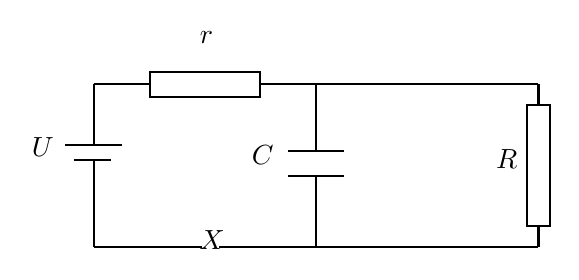
\begin{tikzpicture}[x=0.75pt,y=0.75pt,yscale=-1,xscale=1]
%uncomment if require: \path (0,300); %set diagram left start at 0, and has height of 300

%Straight Lines [id:da992635552977859] 
\draw    (159.43,99.05) -- (266.58,99.05) ;
%Shape: Rectangle [id:dp40515807470760334] 
\draw  [fill={rgb, 255:red, 255; green, 255; blue, 255 }  ,fill opacity=1 ] (186.38,92.98) -- (239.64,92.98) -- (239.64,105.13) -- (186.38,105.13) -- cycle ;
%Straight Lines [id:da9013646240831978] 
\draw    (266.58,131.38) -- (266.58,99.05) ;
%Straight Lines [id:da843756955596408] 
\draw    (266.58,99.05) -- (373.73,99.05) ;
%Straight Lines [id:da6880281635624372] 
\draw    (373.73,177.42) -- (373.73,99.05) ;
%Straight Lines [id:da10033565086863971] 
\draw    (266.58,177.42) -- (373.73,177.42) ;
%Straight Lines [id:da7517210738689919] 
\draw    (219.88,177.42) -- (266.58,177.42) ;
%Straight Lines [id:da6294900742240948] 
\draw    (159.43,128.44) -- (159.43,99.05) ;
%Straight Lines [id:da7676124152868049] 
\draw    (159.43,177.42) -- (159.43,135.3) ;
%Straight Lines [id:da9227393314302665] 
\draw    (145.83,128.44) -- (173.04,128.44) ;
%Straight Lines [id:da4284739815829446] 
\draw    (149.99,135.3) -- (167.79,135.3) ;
%Straight Lines [id:da08072848111989406] 
\draw    (266.58,177.42) -- (266.58,143.13) ;
%Straight Lines [id:da44210756207608326] 
\draw    (252.98,131.38) -- (280.19,131.38) ;
%Straight Lines [id:da8980247380162103] 
\draw    (252.98,143.13) -- (280.19,143.13) ;
%Shape: Rectangle [id:dp25862548825541065] 
\draw  [fill={rgb, 255:red, 255; green, 255; blue, 255 }  ,fill opacity=1 ] (379.3,109.19) -- (379.3,167.28) -- (368.16,167.28) -- (368.16,109.19) -- cycle ;
%Straight Lines [id:da8646847580277894] 
\draw    (159.43,177.42) -- (211.8,177.42) ;


% Text Node
\draw (209.02,168.25) node [anchor=north west][inner sep=0.75pt]    {$X$};
% Text Node
\draw (128.13,123.19) node [anchor=north west][inner sep=0.75pt]    {$U$};
% Text Node
\draw (234.17,127.11) node [anchor=north west][inner sep=0.75pt]    {$C$};
% Text Node
\draw (209.07,72.25) node [anchor=north west][inner sep=0.75pt]    {$r$};
% Text Node
\draw (351.82,129.07) node [anchor=north west][inner sep=0.75pt]    {$R$};


\end{tikzpicture}
\end{center}
Điện trở $R$ chính là thiết bị điện, điện trở $r \ll R$ đặc trưng cho điện trở của dây dẫn và tụ điện có điện dung $C=420\,\mathrm{nF}$ đặc trưng cho trở kháng của dây. Điểm được đánh dấu $X$ trên mạch là một điểm nối tiếp xúc kém, do đó nó sẽ đóng mở mạch theo các chu kì. Mỗi nửa chu kì đóng và mở đều kéo dài $0,001~\mathrm{s}$. Tìm công suất mà nguồn điện cung cấp cho thiết bị điện sau một thời gian rất dài mạch được đóng. Cho rằng nếu điểm tiếp xúc là ổn định (không bị đóng mở theo chu kì) thì công suất cung cấp bởi nguồn sẽ là $P_0 = 30~\mathrm{W}$.
\end{vd}
\begin{loigiai}\[\]
Đầu tiên, chúng ta tính cường độ dòng điện chạy trong mạch. Từ định luật Kirchhoff chúng ta biết rằng dòng điện $I$ chạy qua điện trở $r$ và nguồn là tổng của hai dòng điện $I_C$ và $I_R$ lần lượt chạy qua tụ điện và điện trở $R$. Hiệu điện thế đặt lên hai đầu tụ điện và hai đầu điện trở là bằng nhau, do đó ta có:
   \[R I_R = U_C .\]
Đạo hàm theo thời gian với $C\,\dd U= \dd Q$ ta có:
   \[RC \dot{I}_R = I_C , \]

ở đây dấu chấm ở trên $I_R$ mang ý nghĩa là đạo hàm theo thời gian. Công thức cơ bản cuối cùng mà chúng ta cần là phân bố điện thế trên các điện trở:
    \[U_0 = rI + RI_R .\]

Mỗi khi điểm tiếp xúc $X$ làm hở mạch, tụ điện sẽ phóng điện qua thiết bị. Lúc đó dòng điện qua nguồn $I=0$, nên $I_R=-I_C$ và
    \[-RC \dot{I}_C = I_C .\]

Nghiệm của phương trình là một hàm mũ suy giảm:
    \[ I_{C}^{V}(t) = I_{C}^{V}(0)  e^{-\frac{t}{RC}}.\]

Khi pin được kết nối trở lại ta có:
   \[ R I_R + rI_C + rI_R = U_0,\]

từ đây, đạo hàm theo thời gian ta có:
    \[ \frac{R+r}{RC} I_C + r \dot{I}_C =0,\]

và nghiệm của phương trình là:
  \[I_{C}^{z} = I_{C}^{z} (0) e^{-(\frac{R}{r} +1)\frac{t}{RC}}. \]

Bước tiếp theo là đảm bảo các phương trình này thỏa mãn tính liên tục khi pin được ngắt và đóng. Hiệu điện thế trên tụ điện phải thay đổi liên tục theo thời gian (nếu không sẽ phải tồn tại một dòng năng lượng bằng vô cùng vào và ra khỏi tụ). Hiệu điện thế này được “đo” trên thiết bị điện $R$, do đó dòng điện $I_R$ trên thiết bị cũng là liên tục. Ở thời điểm pin bị ngắt điện
    \[ I_{R}^{z}(T) = I_{R}^{V} (0) . \]

và khi pin được kết nối trở lại
    \[I_{R}^{V}(T) = I_{R}^{z}(0) . \]

Chúng ta có thể tính được cường độ dòng qua điện trở phụ theo hệ phương trình sau đây
  \[ \begin{aligned}  I_{R}^{V} & = - I_{C}^{V}, \\
          I_{R}^{z} &= \dfrac{U_0 - rI_{C}^{z} }{R+ r} . \end{aligned} \]

Thay nghiệm của hệ vào các phương trình phía trước ta có nghiệm cho $I_{C}^{V}(0)$ và $I_{C}^{Z}(0)$ 
  \[  \begin{aligned} \frac{U_0}{r} + \frac{R+r}{r} I_{C}^{V}(0) &= I_{C}^{z} (0) e^{-(\frac{R}{r} +1) \frac{T}{RC}} , \\
    I_{C}^{z}(0) &= \frac{U_0}{r} + \frac{R+r}{r}I_{C}^{V} (0) e^{-\frac{T}{RC}}. \end{aligned}\]

Đồng nhất các phương trình, ta có phương trình cho sự thay đổi điện tích
   \[\frac{R+r}{r}I_{C}^{V} (0) \left(1- e^{-\frac{T}{RC}}\right) = - I_{C}^{z} (0) \left( 1 - e^{-(\frac{R}{r} +1) \frac{T}{RC}}\right) .\]

Từ đây ta giải ra
 \[ I_{C}^{V}(0) = - \frac{U_0}{R+r} \dfrac{1 - e^{-\frac{R+r}{r}\frac{T}{RC}} }{1 - e^{- (\frac{R}{r} +2 ) \frac{T}{RC}} }. \]

và dùng các kết quả trước đó
   \[I_{C}{z} (0) = \frac{U_0}{r} \frac{1- e^{-\frac{T}{RC} }}{1 - e^{-(\frac{R}{r} +2)\frac{T}{RC}}} .\]

Chúng ta có thể thấy dòng phóng điện có có dấu âm, thỏa mãn với cách chọn chiều dòng điện ban đầu.Đây là toàn bộ các phương trình dòng cho đoạn mạch, tiếp theo ta tính đến công suất cung cấp. \\
Công sinh bởi nguồn điện trong một chu kì đóng mở là:
  \[ W =\int_{0}^{T} U_0 I^{z} (t) \dd t + \int_{0}^{T} U_0 I^{V}(t) \dd t = \int_{0}^{T} U_0 I^{z} (t) \dd t. \]

Dòng điện qua nguồn là:
   \[ I^{z} = I_{C}^{z} + I_{R}^{z} = I_{C}^{z} + \frac{U_0 - r I_{C}^{z}}{R+r} , \]

do đó dòng này sinh công:
   \[\begin{aligned}
W &=\frac{U_{0}}{R+r} \int_{0}^{T}\left(U_{0}+R I_{C}^{\mathrm{Z}}(0) \mathrm{e}^{-\left(\frac{R}{r}+1\right) \frac{t}{R C}}\right) \mathrm{d} t=\\
&=\frac{U_{0}}{R+r}\left[U_{0} t-\left(\left(\frac{R}{r}+1\right) \frac{1}{R C}\right)^{-1} R I_{C}^{2}(0) \mathrm{e}^{-\left(\frac{R}{r}+1\right) \frac{t}{R C}}\right]_{0}^{T}=\\
&=\frac{U_{0}}{R+r}\left(U_{0} T+\frac{r R^{2} C}{R+r} I_{C}^{2}(0)\left(1-\mathrm{e}^{-\left(\frac{R}{r}+1\right) \frac{T}{R C}}\right)\right)=\\
&=\frac{U_{0}^{2}}{R+r}\left(T+\frac{R^{2} C}{R+r} \frac{\left(1-\mathrm{e}^{-\frac{T}{R C}}\right)\left(1-\mathrm{e}^{\left.-\left(\frac{R}{r}+1\right) \frac{T}{R C}\right)}\right.}{1-\mathrm{e}^{-\left(\frac{R}{r}+2\right) \frac{T}{R C}}}\right) .
\end{aligned}\]
Để tính công suất trung bình, dùng $P_0 = \frac{U_0^2}{R+r}$ ta có:
  \[ P = \frac{W}{2T} = \frac{P_0}{2} \left(1 + \frac{R^2 C}{T(R+r)} \frac{\left(1 - e^{-\frac{T}{RC} }\right) \left(1 - e^{-(\frac{R}{r} +1) \frac{T}{RC}}\right) }{1 - e^{-(\frac{R}{r} +2) \frac{T}{RC}}} \right).\]

Hơn nữa, lại có $R \gg r$ ta rút gọn lại được thành
    \[ P \approx \frac{P_0}{2} \left( 1 + \frac{RC}{T} \left(1 - e^{-\frac{T}{RC}}\right)\right) .\]

Chúng ta có thể thấy, công suất sẽ xấp xỉ $P_0/2$ với $RC/T$ nhỏ và tiến đến $P_0$ khi $RC/T$ tiến đến vô cùng. Do đó, khi tụ điện có điện dung nhỏ, mạch điện sẽ không khác đáng kể so với việc không có tụ điện, và ngược lại, nếu tụ điện có điện dung lớn, mạch điện xấp xỉ luôn đóng mà không bị ngắt. Đây là một công dụng phổ biến của tụ điện $-$ giữ cho mạch điện không bị sụt thế đột ngột khi nguồn cấp xuất hiện thăng giáng. Biết điện thế và công suất mạch khi mạch điện luôn được đóng kín, chúng ta có điện trở của thiết bị:
      \[ R \approx \frac{U_0^2}{P_0} ,\]
và do đó công suất như đề bài yêu cầu:
         \[ P =\frac{P_0}{2} + \frac{U_0^2}{2T} \left( 1 - e^{-\frac{P_0T}{U_0^2 C}} \right) = 18,0 ~\mathrm{W} . \]

\end{loigiai}

\begin{vd}[Quá trình cảm nhận các tín hiệu điện] %Prob2 IPhO 2002
Một số sinh vật biển có khả năng phát hiện được các sinh vật khác từ một khoảng cách nào đó dựa trên dòng điện mà các sinh vật đó sinh ra trong quá trình thở hoặc các quá trình co cơ khác. Một số cá săn mồi dùng tín hiệu điện ấy để định vị con mồi ngay cả khi con mồi vùi mình dưới cát.\\
Cơ chế vật lý của sự sinh ra dòng điện từ con mồi và cách cá săn mồi phát hiện dòng điện ấy đã được mô hình hoá trên hình 1. Dòng điện sinh ra bởi con mồi chạy giữa hai hình cầu có điện thế dương và âm trên thân con mồi. Khoảng cách giữa các tâm của hai hình cầu đó là $l_s$ , mỗi hình cầu có bán kính là $r_s$ rất nhỏ so với $l_s$. Điện trở suất của nước biển là $\rho$. Cho rằng điện trở suất của thân con mồi có cùng giá trị với nước biển bao quanh nó. Khi ấy, trên hình vẽ, ta có thể không xét đến bờ phân cách giữa con mồi và môi trường xung quanh.
\begin{center}
\tikzset{every picture/.style={line width=0.75pt}} %set default line width to 0.75pt        
\begin{tikzpicture}[x=0.75pt,y=0.75pt,yscale=-1,xscale=1]
%uncomment if require: \path (0,528); %set diagram left start at 0, and has height of 528

%Shape: Resistor [id:dp6250723636150566] 
\draw   (348.73,145.13) -- (355.9,145.13) -- (357.49,130.74) -- (360.68,159.52) -- (363.87,130.74) -- (367.05,159.52) -- (370.24,130.74) -- (373.42,159.52) -- (376.61,130.74) -- (379.79,159.52) -- (381.39,145.13) -- (388.55,145.13) ;
%Straight Lines [id:da6937081601394308] 
\draw    (388.55,145.13) -- (413.17,145.13) ;
%Straight Lines [id:da5454777120579675] 
\draw    (324.12,145.13) -- (348.73,145.13) ;
%Straight Lines [id:da10639832468286481] 
\draw    (413.17,145.13) -- (413.17,170.56) ;
%Straight Lines [id:da678094125261552] 
\draw    (324.12,145.13) -- (324.12,170.56) ;
%Shape: Circle [id:dp438142038358325] 
\draw   (316.15,178.53) .. controls (316.15,174.13) and (319.72,170.56) .. (324.12,170.56) .. controls (328.51,170.56) and (332.08,174.13) .. (332.08,178.53) .. controls (332.08,182.93) and (328.51,186.49) .. (324.12,186.49) .. controls (319.72,186.49) and (316.15,182.93) .. (316.15,178.53) -- cycle ;
%Shape: Circle [id:dp006011042445173365] 
\draw   (405.21,178.53) .. controls (405.21,174.13) and (408.77,170.56) .. (413.17,170.56) .. controls (417.57,170.56) and (421.13,174.13) .. (421.13,178.53) .. controls (421.13,182.93) and (417.57,186.49) .. (413.17,186.49) .. controls (408.77,186.49) and (405.21,182.93) .. (405.21,178.53) -- cycle ;
%Shape: Circle [id:dp8565224096581663] 
\draw  [fill={rgb, 255:red, 0; green, 0; blue, 0 }  ,fill opacity=1 ] (303.84,353.74) .. controls (303.84,349.34) and (307.41,345.78) .. (311.81,345.78) .. controls (316.21,345.78) and (319.77,349.34) .. (319.77,353.74) .. controls (319.77,358.14) and (316.21,361.7) .. (311.81,361.7) .. controls (307.41,361.7) and (303.84,358.14) .. (303.84,353.74) -- cycle ;
%Shape: Ellipse [id:dp9292507440846232] 
\draw  [fill={rgb, 255:red, 0; green, 0; blue, 0 }  ,fill opacity=1 ] (418.96,354.46) .. controls (418.96,350.07) and (422.53,346.5) .. (426.93,346.5) .. controls (431.33,346.5) and (434.89,350.07) .. (434.89,354.46) .. controls (434.89,358.86) and (431.33,362.43) .. (426.93,362.43) .. controls (422.53,362.43) and (418.96,358.86) .. (418.96,354.46) -- cycle ;
\draw   (421.38,340.04) -- (432.6,340.04)(426.99,334.43) -- (426.99,345.66) ;
%Straight Lines [id:da5447229893783567] 
\draw    (305.65,339.62) -- (319.77,339.62) ;
%Straight Lines [id:da23567329313537821] 
\draw  [dash pattern={on 4.5pt off 4.5pt}]  (205.74,354.46) -- (512.24,354.46) ;
%Straight Lines [id:da12542128129149144] 
\draw  [dash pattern={on 4.5pt off 4.5pt}]  (368.64,369.08) -- (368.64,178.53) ;
%Straight Lines [id:da6280856311331429] 
\draw  [dash pattern={on 4.5pt off 4.5pt}]  (332.08,178.53) -- (405.21,178.53) ;
%Straight Lines [id:da7900095397375582] 
\draw    (327.12,201.38) -- (410.17,201.38) ;
\draw [shift={(413.17,201.38)}, rotate = 180] [fill={rgb, 255:red, 0; green, 0; blue, 0 }  ][line width=0.08]  [draw opacity=0] (10.72,-5.15) -- (0,0) -- (10.72,5.15) -- (7.12,0) -- cycle    ;
\draw [shift={(324.12,201.38)}, rotate = 0] [fill={rgb, 255:red, 0; green, 0; blue, 0 }  ][line width=0.08]  [draw opacity=0] (10.72,-5.15) -- (0,0) -- (10.72,5.15) -- (7.12,0) -- cycle    ;
%Straight Lines [id:da5935848877927736] 
\draw    (314.81,395.25) -- (423.93,395.25) ;
\draw [shift={(426.93,395.25)}, rotate = 180] [fill={rgb, 255:red, 0; green, 0; blue, 0 }  ][line width=0.08]  [draw opacity=0] (10.72,-5.15) -- (0,0) -- (10.72,5.15) -- (7.12,0) -- cycle    ;
\draw [shift={(311.81,395.25)}, rotate = 0] [fill={rgb, 255:red, 0; green, 0; blue, 0 }  ][line width=0.08]  [draw opacity=0] (10.72,-5.15) -- (0,0) -- (10.72,5.15) -- (7.12,0) -- cycle    ;
%Straight Lines [id:da7865025666050354] 
\draw    (324.12,189.39) -- (324.12,214.82) ;
%Straight Lines [id:da19240439653140862] 
\draw    (413.17,188.66) -- (413.17,214.1) ;
%Straight Lines [id:da3565828698213691] 
\draw    (311.81,373.29) -- (311.81,398.72) ;
%Straight Lines [id:da01048176854550853] 
\draw    (426.93,372.93) -- (426.93,398.36) ;
%Curve Lines [id:da31620849287150943] 
\draw    (111.5,175.08) .. controls (196.5,138.08) and (434.17,86.08) .. (532.17,174.75) ;
%Curve Lines [id:da8672347428077531] 
\draw    (111.5,175.08) .. controls (163.67,203.42) and (444.67,275.25) .. (532.17,174.75) ;
%Curve Lines [id:da4535109370826258] 
\draw    (227.5,354.33) .. controls (284.5,328.08) and (423.5,304.08) .. (477,354.08) ;
%Curve Lines [id:da6653411087326846] 
\draw    (227.5,354.33) .. controls (260.5,371.08) and (420,412.08) .. (477,354.08) ;

% Text Node
\draw (376.08,207.04) node [anchor=north west][inner sep=0.75pt]    {$l_{d}$};
% Text Node
\draw (363.15,101.07) node [anchor=north west][inner sep=0.75pt]    {$R_{d}$};
% Text Node
\draw (364.98,401.9) node [anchor=north west][inner sep=0.75pt]    {$l_{s}$};
% Text Node
\draw (375.36,261.23) node [anchor=north west][inner sep=0.75pt]    {$y$};
% Text Node
\draw (364.68,159.42) node [anchor=north west][inner sep=0.75pt]    {$P$};
% Text Node
\draw (492.5,122.33) node [anchor=north west][inner sep=0.75pt]   [align=left] {Cá săn mồi};
% Text Node
\draw (447.5,313.33) node [anchor=north west][inner sep=0.75pt]   [align=left] {con mồi};
\end{tikzpicture}\\
    Hình 1 . Một mô hình diễn tả cách cá săn mồi phát hiện công suất điện từ con mồi phát ra.
\end{center}
Để mô tả cách cá săn mồi phát hiện công suất điện từ con mồi phát ra, ta cũng dùng mô hình tương tự như trên đối với đầu thu điện. Đầu thu là hai quả cầu ở trên thân cá săn mồi và tiếp xúc với môi trường nước biển bao quanh. Cặp quả cầu này nằm song song với cặp quả cầu trên thân con mồi. Hai quả cầu đó cách  nhau khoảng $l_d$ và mỗi quả có bán kính là $r_d$ rất nhỏ so với $l_d$. Trong trường hợp này, tâm của đầu thu nằm ngay trên nguồn phát dòng điện và cách nó khoảng $y$. Đường nối tâm của hai quả cầu song song với điện trường tại đấy, như đã vẽ trên hình 1. Cả $l_s$ lẫn $l_d$ đều rất nhỏ so với $y$. Cường độ điện trường dọc theo đường nối $2$ quả cầu xem như có giá trị không đổi. Như thế, đầu thu khép kín mạch điện tạo bởi con mồi, môi trường nước xung quanh và con cá săn mồi như đã vẽ trên hình 2.
\begin{center}
\tikzset{every picture/.style={line width=0.75pt}} %set default line width to 0.75pt        

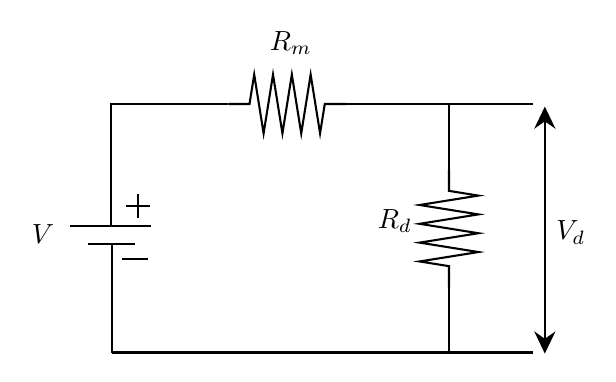
\begin{tikzpicture}[x=0.75pt,y=0.75pt,yscale=-1,xscale=1]
%uncomment if require: \path (0,502); %set diagram left start at 0, and has height of 502

%Shape: Resistor [id:dp6031376192161455] 
\draw   (277,117.83) -- (287.2,117.83) -- (289.47,103.67) -- (294,132) -- (298.53,103.67) -- (303.07,132) -- (307.6,103.67) -- (312.13,132) -- (316.67,103.67) -- (321.2,132) -- (323.47,117.83) -- (333.67,117.83) ;
%Shape: Resistor [id:dp01885050926410048] 
\draw   (383.33,149.5) -- (383.33,159.7) -- (397.5,161.97) -- (369.17,166.5) -- (397.5,171.03) -- (369.17,175.57) -- (397.5,180.1) -- (369.17,184.63) -- (397.5,189.17) -- (369.17,193.7) -- (383.33,195.97) -- (383.33,206.17) ;
%Shape: Right Angle [id:dp3330470857496082] 
\draw   (333.67,117.83) -- (383.33,117.83) -- (383.33,149.5) ;
%Shape: Right Angle [id:dp5522408490603117] 
\draw   (383.33,206.17) -- (383.33,237.58) -- (220.83,237.58) ;
%Straight Lines [id:da5649548194013958] 
\draw    (220.83,185.08) -- (220.83,237.58) ;
%Shape: Right Angle [id:dp4263793688907498] 
\draw   (220.33,176.58) -- (220.33,117.83) -- (277,117.83) ;
%Straight Lines [id:da5748733114306972] 
\draw    (200.96,176.58) -- (239.71,176.58) ;
%Straight Lines [id:da9774571131081751] 
\draw    (209.4,185.08) -- (232.27,185.08) ;
\draw   (227.83,166.96) -- (239.08,166.96)(233.46,161.33) -- (233.46,172.58) ;
%Straight Lines [id:da24253384653698062] 
\draw    (225.9,192.58) -- (238.33,192.58) ;
%Straight Lines [id:da26726830275677926] 
\draw    (429.5,122.08) -- (429.5,235.08) ;
\draw [shift={(429.5,238.08)}, rotate = 270] [fill={rgb, 255:red, 0; green, 0; blue, 0 }  ][line width=0.08]  [draw opacity=0] (10.72,-5.15) -- (0,0) -- (10.72,5.15) -- (7.12,0) -- cycle    ;
\draw [shift={(429.5,119.08)}, rotate = 90] [fill={rgb, 255:red, 0; green, 0; blue, 0 }  ][line width=0.08]  [draw opacity=0] (10.72,-5.15) -- (0,0) -- (10.72,5.15) -- (7.12,0) -- cycle    ;
%Straight Lines [id:da07378917413551034] 
\draw    (383.33,237.58) -- (423.83,237.58) ;
%Straight Lines [id:da24601213846576897] 
\draw    (383.33,117.83) -- (423.83,117.83) ;

% Text Node
\draw (180.83,174.23) node [anchor=north west][inner sep=0.75pt]    {$V$};
% Text Node
\draw (295.5,81.57) node [anchor=north west][inner sep=0.75pt]    {$R_{m}$};
% Text Node
\draw (347.5,167.07) node [anchor=north west][inner sep=0.75pt]    {$R_{d}$};
% Text Node
\draw (433.5,172.73) node [anchor=north west][inner sep=0.75pt]    {$V_{d}$};
\end{tikzpicture}
    \\Hình 2. Mạch kín tương đương gồm cá săn mồi, con mồi và nước biển bao quanh.
\end{center}
Trên hình vẽ, $V$ là hiệu điện thế giữa hai quả cầu của đầu thu do điện trường của con mồi cảm ứng mà có, $R_m$ là điện trở trong gây ra bởi nước biển bao quanh. Ngoài ra, $V_d$ và $R_d$ lần lượt là hiệu điện thế giữa hai quả cầu của đầu 
thu và điện trở của đầu thu trên cá săn mồi.\\
\begin{enumerate}[1)]
    \item  Hãy xác định vector mật độ dòng $\ot j$ (dòng điện qua một đơn vị diện tích) được gây ra bởi một điểm nguồn phát dòng điện $I_s$ tại một điểm cách nó khoảng $r$ trong môi trường dẫn điện rộng vô hạn. 
    \item Dựa trên định luật $\ot{E} = \rho \ot{j}$, hãy xác định cường độ địện trường $\ot{E_p}$ tại điểm giữa đường nối hai quả cầu của đầu thu (điểm $P$) khi biết dòng $I_s$ chạy giữa hai quả cầu trên thân con mồi.
    \item Với cùng dòng điện $I_s$, hãy xác định hiệu điện thế $(V_s)$ giữa hai quả cầu phát điện trên thân con mồi. Hãy xác định điện trở giữa hai quả cầu phát điện $(R_s)$ và công suất sinh ra bởi nguồn $(P_s)$.
    \item Xác định $R_m$, $V_d$ trên hình 2 và tính công suất truyền từ nguồn phát điện đến đầu thu $(P_d)$. 
    \item Hãy xác định giá trị tối ưu của $R_d$ để cho công suất mà cá săn mồi phát hiện được đạt cực đại và xác định công suất cực đại ấy.
\end{enumerate}
\end{vd}
\begin{loigiai}
\begin{enumerate}[1)]
    \item Khi nguồn dòng điểm $I_s$ ở trong môi trường đẳng hướng vô hạn, vector mật độ dòng điện ở khoảng cách $r$ tính từ nguồn điểm là:
    \[\ot{j} = \dfrac{I_{s}}{4 \pi r^{3}} \ot r .\]
    \item Giả sử rằng điện trở suất của cơ thể con mồi và môi trường nước biển xung quanh là như nhau, nghĩa là loại bỏ ranh giới xung quanh con mồi, hai quả cầu được coi như là các vật đẳng hướng vô hạn với điện trở suất $\rho$. Khi một quả cầu nhỏ tạo ra dòng điện với một tỉ lệ $I_{s}$, mật độ thông lượng dòng điện ở khoảng cách $r$ tính từ tâm của quả cầu cũng là
    \[\ot{j} = \dfrac{I_{s}}{4 \pi r^{3}} \ot r .\]
    Điện trở suất của nước biển là $\rho$, do đó cường độ điện trường tại điềm cách tâm quả cầu $r$ là:
    \[\ot{E}\tron{\ot r} = \rho \ot j = \dfrac{\rho I_{s}}{4 \pi r^{3}} \ot r .\]
    Trong mô hình này, chúng ta có hai quả cầu nhỏ. Một quả có điện thế dương so với quả kia, do đó có dòng $I_s$ chạy từ quả cầu tích điện dương tới quả cầu tích âm. Chúng được phân cách nhau bởi $I_s$.
    \begin{center}
        

\tikzset{every picture/.style={line width=0.75pt}} %set default line width to 0.75pt        

\begin{tikzpicture}[x=0.75pt,y=0.75pt,yscale=-1,xscale=1]
%uncomment if require: \path (0,510); %set diagram left start at 0, and has height of 510

%Shape: Circle [id:dp19698912476050778] 
\draw  [fill={rgb, 255:red, 0; green, 0; blue, 0 }  ,fill opacity=1 ] (235.84,298.91) .. controls (235.84,294.51) and (239.41,290.94) .. (243.81,290.94) .. controls (248.21,290.94) and (251.77,294.51) .. (251.77,298.91) .. controls (251.77,303.31) and (248.21,306.87) .. (243.81,306.87) .. controls (239.41,306.87) and (235.84,303.31) .. (235.84,298.91) -- cycle ;
%Shape: Ellipse [id:dp8872597777432196] 
\draw  [fill={rgb, 255:red, 0; green, 0; blue, 0 }  ,fill opacity=1 ] (350.96,299.63) .. controls (350.96,295.23) and (354.53,291.67) .. (358.93,291.67) .. controls (363.33,291.67) and (366.89,295.23) .. (366.89,299.63) .. controls (366.89,304.03) and (363.33,307.6) .. (358.93,307.6) .. controls (354.53,307.6) and (350.96,304.03) .. (350.96,299.63) -- cycle ;
\draw   (353.38,285.21) -- (364.6,285.21)(358.99,279.6) -- (358.99,290.82) ;
%Straight Lines [id:da7123421579712839] 
\draw    (237.65,284.79) -- (251.77,284.79) ;
%Straight Lines [id:da935547014999208] 
\draw  [dash pattern={on 4.5pt off 4.5pt}]  (137.74,299.63) -- (444.24,299.63) ;
%Straight Lines [id:da6246118276516146] 
\draw  [dash pattern={on 4.5pt off 4.5pt}]  (300.64,314.25) -- (300.64,123.7) ;
%Straight Lines [id:da48446922723622654] 
\draw    (243.81,308.46) -- (243.81,320) ;
%Curve Lines [id:da6640680535268084] 
\draw    (159.5,299.5) .. controls (216.5,273.25) and (355.5,249.25) .. (409,299.25) ;
%Curve Lines [id:da9078645717603522] 
\draw    (159.5,299.5) .. controls (192.5,316.25) and (352,357.25) .. (409,299.25) ;
%Straight Lines [id:da8795076103514246] 
\draw  [dash pattern={on 4.5pt off 4.5pt}]  (243.81,298.91) -- (300.64,123.7) ;
%Straight Lines [id:da5462344759239897] 
\draw  [dash pattern={on 4.5pt off 4.5pt}]  (358.93,299.63) -- (300.64,123.7) ;
%Straight Lines [id:da49158962946942064] 
\draw [line width=1.5]    (300.64,123.7) -- (279.39,189.94) ;
\draw [shift={(278.17,193.75)}, rotate = 287.79] [fill={rgb, 255:red, 0; green, 0; blue, 0 }  ][line width=0.08]  [draw opacity=0] (13.4,-6.43) -- (0,0) -- (13.4,6.44) -- (8.9,0) -- cycle    ;
%Straight Lines [id:da5498110379576178] 
\draw [line width=1.5]    (300.64,123.7) -- (279.17,60.34) ;
\draw [shift={(277.89,56.56)}, rotate = 431.28] [fill={rgb, 255:red, 0; green, 0; blue, 0 }  ][line width=0.08]  [draw opacity=0] (13.4,-6.43) -- (0,0) -- (13.4,6.44) -- (8.9,0) -- cycle    ;
%Straight Lines [id:da643688473273047] 
\draw    (358.93,308.6) -- (358.93,320.14) ;

% Text Node
\draw (307.36,206.4) node [anchor=north west][inner sep=0.75pt]    {$y$};
% Text Node
\draw (379.5,258.5) node [anchor=north west][inner sep=0.75pt]   [align=left] {con mồi};
% Text Node
\draw (308,112.4) node [anchor=north west][inner sep=0.75pt]    {$P$};
% Text Node
\draw (280,338.07) node [anchor=north west][inner sep=0.75pt]    {$x=0$};
% Text Node
\draw (339,324.07) node [anchor=north west][inner sep=0.75pt]    {$x = + \dfrac{l_{s}}{2}$};
% Text Node
\draw (200,324.07) node [anchor=north west][inner sep=0.75pt]    {$x = - \dfrac{l_{s}}{2}$};
\end{tikzpicture}
    \end{center}
    Cường độ điện trường tại điểm ${P}(0, {y})$ là:
    \[\begin{aligned}
    \ot{E_p} &= \ot{E_+} + \ot{E_-}\\
    &= \dfrac{\rho I_{s}}{4 \pi}\left[\dfrac{1}{\left(\left(\dfrac{l_{s}}{2}\right)^{2}+y^{2}\right)^{\dfrac{3}{2}}}\left(-\dfrac{l_{s}}{2} \hat{i} +y \hat{j}\right) + \dfrac{1}{\left(\left(\dfrac{l_{s}}{2}\right)^{2}+y^{2}\right)^{\dfrac{3}{2}}}\left(-\dfrac{l_{s}}{2} \hat{i} - y \hat{j}\right)\right]\\
    &= \dfrac{\rho I_{s}}{4 \pi}\dfrac{l_{s}(-\hat{i})}{\left(\left(\dfrac{l_{s}}{2}\right)^{2} + y^{2}\right)^{\dfrac{3}{2}}}
    \end{aligned}\]
    \[\ot{E}_{p} \approx \dfrac{\rho I_{s} l_{s}}{4 \pi y^{3}}\tron{-\hat{i}} \quad \text{vì} \quad {l_s} \ll {y} .\]
    
    \item Cường độ điện trường dọc theo trục giữa hai quả cầu là:
    \[
\ot{E}(x) = \dfrac{\rho I_{s}}{4 \pi}\tron{\dfrac{1}{\left(x-\dfrac{l_{s}}{2}\right)^{2}}+\dfrac{1}{\tron{x+\dfrac{l_{s}}{2}}^{2}}}\tron{-\hat{i}}
\]
Hiệu điện thế tạo ra dòng $I_{s}$ đã cho là:

\[\begin{aligned}
V_{s} &= \Delta V = V_{+} - V_{-} = -\int^{\tron{\frac{l_s}{2} - r_{s}}}_{\tron{-\frac{l_s}{2} + r_{s}}}    \ot{E}(x) \dd x \\
&= - \dfrac{\rho I_{s}}{4 \pi} \int^{\tron{\frac{l_s}{2} - r_{s}}}_{\tron{-\frac{l_s}{2} + r_{s}}} \tron{\dfrac{1}{\tron{x-\dfrac{l_s}{2}}^{2}}+\dfrac{1}{\tron{x+\dfrac{l_s}{2}}^{2}}}\tron{-\hat{i}}\tron{\hat{i} \dd x}\\
&= \dfrac{\rho l_{s}}{4 \pi}\left[\dfrac{1}{-2+1}\tron{\dfrac{1}{\tron{\dfrac{l_{s}}{2}-r_{s}-\dfrac{l_{s}}{2}}}-\dfrac{1}{\tron{-\dfrac{l_{s}}{2}+r_{s}-\dfrac{l_{s}}{2}}}}\right.\\
&+ \left.  \dfrac{1}{-2+1}\tron{\dfrac{1}{\tron{\dfrac{l_{s}}{2}-r_{s}+\dfrac{l_{s}}{2}}}-\dfrac{1}{\tron{-\dfrac{l_{s}}{2}+r_{s}+\dfrac{l_{s}}{2}}}}\right]\\
&= \dfrac{\rho I_{s}}{4 \pi}\left(\dfrac{2}{r_{s}}-\dfrac{2}{l_{s}-r_{s}}\right) = \dfrac{2 \rho I_{s}}{4 \pi}\left(\dfrac{l_{s}-r_{s}-r_{s}}{\left(l_{s}-r_{s}\right) r_{s}}\right) = \dfrac{\rho I_{s}}{2 \pi r_{s}}\left(\dfrac{l_{s}-2 r_{s}}{l_{s}-r_{s}}\right).
\end{aligned}\]
Hay: \[V_s = \Delta V \approx \dfrac{\rho I_{s}}{2 \pi r_{s}} \quad \text{vì} \quad l_s \gg r_s .\]
Điện trở giữa hai quả cầu là:
\[R_s = \dfrac{V_s}{I_s} = \dfrac{\rho}{2\pi r_s}.\]
Công suất của nguồn:
\[P = I_sV_s = \dfrac{\rho I_s^2}{2\pi r_s}.\]
\item ${V}$ là hiệu điện thế giữa quả cầu của máy dò do điện trường gây ra bởi con mồi, $R_{m}$ là điện trở trong do nước biển xung quanh gây ra. $V_{d}$ và $R_{d}$ lần lượt là hiệu điện thế giữa quả cầu thu và điện trở của máy thu bên trong con cá săn mồi
và $i_{d}$ là dòng điện chạy trong trạng thái đóng mạch.
\begin{center}
    

\tikzset{every picture/.style={line width=0.75pt}} %set default line width to 0.75pt        

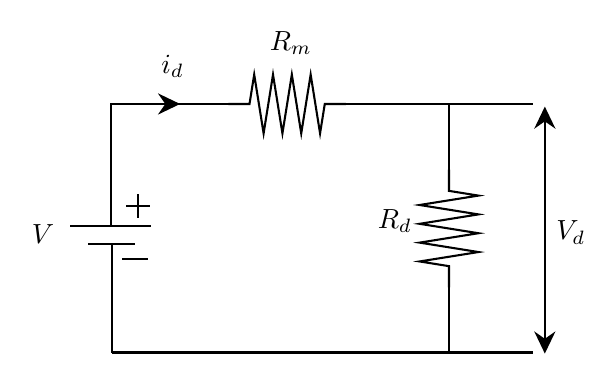
\begin{tikzpicture}[x=0.75pt,y=0.75pt,yscale=-1,xscale=1]
%uncomment if require: \path (0,502); %set diagram left start at 0, and has height of 502

%Shape: Resistor [id:dp6031376192161455] 
\draw   (277,117.83) -- (287.2,117.83) -- (289.47,103.67) -- (294,132) -- (298.53,103.67) -- (303.07,132) -- (307.6,103.67) -- (312.13,132) -- (316.67,103.67) -- (321.2,132) -- (323.47,117.83) -- (333.67,117.83) ;
%Shape: Resistor [id:dp01885050926410048] 
\draw   (383.33,149.5) -- (383.33,159.7) -- (397.5,161.97) -- (369.17,166.5) -- (397.5,171.03) -- (369.17,175.57) -- (397.5,180.1) -- (369.17,184.63) -- (397.5,189.17) -- (369.17,193.7) -- (383.33,195.97) -- (383.33,206.17) ;
%Shape: Right Angle [id:dp3330470857496082] 
\draw   (333.67,117.83) -- (383.33,117.83) -- (383.33,149.5) ;
%Shape: Right Angle [id:dp5522408490603117] 
\draw   (383.33,206.17) -- (383.33,237.58) -- (220.83,237.58) ;
%Straight Lines [id:da5649548194013958] 
\draw    (220.83,185.08) -- (220.83,237.58) ;
%Shape: Right Angle [id:dp4263793688907498] 
\draw   (220.33,176.58) -- (220.33,117.83) -- (277,117.83) ;
%Straight Lines [id:da5748733114306972] 
\draw    (200.96,176.58) -- (239.71,176.58) ;
%Straight Lines [id:da9774571131081751] 
\draw    (209.4,185.08) -- (232.27,185.08) ;
\draw   (227.83,166.96) -- (239.08,166.96)(233.46,161.33) -- (233.46,172.58) ;
%Straight Lines [id:da24253384653698062] 
\draw    (225.9,192.58) -- (238.33,192.58) ;
%Straight Lines [id:da26726830275677926] 
\draw    (429.5,122.08) -- (429.5,235.08) ;
\draw [shift={(429.5,238.08)}, rotate = 270] [fill={rgb, 255:red, 0; green, 0; blue, 0 }  ][line width=0.08]  [draw opacity=0] (10.72,-5.15) -- (0,0) -- (10.72,5.15) -- (7.12,0) -- cycle    ;
\draw [shift={(429.5,119.08)}, rotate = 90] [fill={rgb, 255:red, 0; green, 0; blue, 0 }  ][line width=0.08]  [draw opacity=0] (10.72,-5.15) -- (0,0) -- (10.72,5.15) -- (7.12,0) -- cycle    ;
%Straight Lines [id:da07378917413551034] 
\draw    (383.33,237.58) -- (423.83,237.58) ;
%Straight Lines [id:da24601213846576897] 
\draw    (383.33,117.83) -- (423.83,117.83) ;
%Straight Lines [id:da5741858825472315] 
\draw    (220.33,117.83) -- (287.2,117.83) ;
\draw [shift={(253.77,117.83)}, rotate = 180] [fill={rgb, 255:red, 0; green, 0; blue, 0 }  ][line width=0.08]  [draw opacity=0] (10.72,-5.15) -- (0,0) -- (10.72,5.15) -- (7.12,0) -- cycle    ;

% Text Node
\draw (180.83,174.23) node [anchor=north west][inner sep=0.75pt]    {$V$};
% Text Node
\draw (295.5,81.57) node [anchor=north west][inner sep=0.75pt]    {$R_{m}$};
% Text Node
\draw (347.5,167.07) node [anchor=north west][inner sep=0.75pt]    {$R_{d}$};
% Text Node
\draw (433.5,172.73) node [anchor=north west][inner sep=0.75pt]    {$V_{d}$};
% Text Node
\draw (243.22,92.96) node [anchor=north west][inner sep=0.75pt]    {$i_{d}$};
\end{tikzpicture}
\end{center}
\begin{center}
    

\tikzset{every picture/.style={line width=0.75pt}} %set default line width to 0.75pt        

\begin{tikzpicture}[x=0.75pt,y=0.75pt,yscale=-1,xscale=1]
%uncomment if require: \path (0,528); %set diagram left start at 0, and has height of 528

%Shape: Resistor [id:dp6250723636150566] 
\draw   (348.73,145.13) -- (355.9,145.13) -- (357.49,130.74) -- (360.68,159.52) -- (363.87,130.74) -- (367.05,159.52) -- (370.24,130.74) -- (373.42,159.52) -- (376.61,130.74) -- (379.79,159.52) -- (381.39,145.13) -- (388.55,145.13) ;
%Straight Lines [id:da6937081601394308] 
\draw    (388.55,145.13) -- (413.17,145.13) ;
%Straight Lines [id:da5454777120579675] 
\draw    (324.12,145.13) -- (348.73,145.13) ;
%Straight Lines [id:da10639832468286481] 
\draw    (413.17,145.13) -- (413.17,170.56) ;
%Straight Lines [id:da678094125261552] 
\draw    (324.12,145.13) -- (324.12,170.56) ;
%Shape: Circle [id:dp438142038358325] 
\draw   (316.15,178.53) .. controls (316.15,174.13) and (319.72,170.56) .. (324.12,170.56) .. controls (328.51,170.56) and (332.08,174.13) .. (332.08,178.53) .. controls (332.08,182.93) and (328.51,186.49) .. (324.12,186.49) .. controls (319.72,186.49) and (316.15,182.93) .. (316.15,178.53) -- cycle ;
%Shape: Circle [id:dp006011042445173365] 
\draw   (405.21,178.53) .. controls (405.21,174.13) and (408.77,170.56) .. (413.17,170.56) .. controls (417.57,170.56) and (421.13,174.13) .. (421.13,178.53) .. controls (421.13,182.93) and (417.57,186.49) .. (413.17,186.49) .. controls (408.77,186.49) and (405.21,182.93) .. (405.21,178.53) -- cycle ;
%Shape: Circle [id:dp8565224096581663] 
\draw  [fill={rgb, 255:red, 0; green, 0; blue, 0 }  ,fill opacity=1 ] (303.84,353.74) .. controls (303.84,349.34) and (307.41,345.78) .. (311.81,345.78) .. controls (316.21,345.78) and (319.77,349.34) .. (319.77,353.74) .. controls (319.77,358.14) and (316.21,361.7) .. (311.81,361.7) .. controls (307.41,361.7) and (303.84,358.14) .. (303.84,353.74) -- cycle ;
%Shape: Ellipse [id:dp9292507440846232] 
\draw  [fill={rgb, 255:red, 0; green, 0; blue, 0 }  ,fill opacity=1 ] (418.96,354.46) .. controls (418.96,350.07) and (422.53,346.5) .. (426.93,346.5) .. controls (431.33,346.5) and (434.89,350.07) .. (434.89,354.46) .. controls (434.89,358.86) and (431.33,362.43) .. (426.93,362.43) .. controls (422.53,362.43) and (418.96,358.86) .. (418.96,354.46) -- cycle ;
\draw   (421.38,340.04) -- (432.6,340.04)(426.99,334.43) -- (426.99,345.66) ;
%Straight Lines [id:da5447229893783567] 
\draw    (305.65,339.62) -- (319.77,339.62) ;
%Straight Lines [id:da23567329313537821] 
\draw  [dash pattern={on 4.5pt off 4.5pt}]  (205.74,354.46) -- (512.24,354.46) ;
%Straight Lines [id:da12542128129149144] 
\draw  [dash pattern={on 4.5pt off 4.5pt}]  (368.64,369.08) -- (368.64,178.53) ;
%Straight Lines [id:da6280856311331429] 
\draw  [dash pattern={on 4.5pt off 4.5pt}]  (332.08,178.53) -- (405.21,178.53) ;
%Straight Lines [id:da7900095397375582] 
\draw    (327.12,201.38) -- (410.17,201.38) ;
\draw [shift={(413.17,201.38)}, rotate = 180] [fill={rgb, 255:red, 0; green, 0; blue, 0 }  ][line width=0.08]  [draw opacity=0] (10.72,-5.15) -- (0,0) -- (10.72,5.15) -- (7.12,0) -- cycle    ;
\draw [shift={(324.12,201.38)}, rotate = 0] [fill={rgb, 255:red, 0; green, 0; blue, 0 }  ][line width=0.08]  [draw opacity=0] (10.72,-5.15) -- (0,0) -- (10.72,5.15) -- (7.12,0) -- cycle    ;
%Straight Lines [id:da5935848877927736] 
\draw    (314.81,395.25) -- (423.93,395.25) ;
\draw [shift={(426.93,395.25)}, rotate = 180] [fill={rgb, 255:red, 0; green, 0; blue, 0 }  ][line width=0.08]  [draw opacity=0] (10.72,-5.15) -- (0,0) -- (10.72,5.15) -- (7.12,0) -- cycle    ;
\draw [shift={(311.81,395.25)}, rotate = 0] [fill={rgb, 255:red, 0; green, 0; blue, 0 }  ][line width=0.08]  [draw opacity=0] (10.72,-5.15) -- (0,0) -- (10.72,5.15) -- (7.12,0) -- cycle    ;
%Straight Lines [id:da7865025666050354] 
\draw    (324.12,189.39) -- (324.12,214.82) ;
%Straight Lines [id:da19240439653140862] 
\draw    (413.17,188.66) -- (413.17,214.1) ;
%Straight Lines [id:da3565828698213691] 
\draw    (311.81,373.29) -- (311.81,398.72) ;
%Straight Lines [id:da01048176854550853] 
\draw    (426.93,372.93) -- (426.93,398.36) ;
%Curve Lines [id:da31620849287150943] 
\draw    (111.5,175.08) .. controls (196.5,138.08) and (434.17,86.08) .. (532.17,174.75) ;
%Curve Lines [id:da8672347428077531] 
\draw    (111.5,175.08) .. controls (163.67,203.42) and (444.67,275.25) .. (532.17,174.75) ;
%Curve Lines [id:da4535109370826258] 
\draw    (227.5,354.33) .. controls (284.5,328.08) and (423.5,304.08) .. (477,354.08) ;
%Curve Lines [id:da6653411087326846] 
\draw    (227.5,354.33) .. controls (260.5,371.08) and (420,412.08) .. (477,354.08) ;

% Text Node
\draw (376.08,207.04) node [anchor=north west][inner sep=0.75pt]    {$l_{d}$};
% Text Node
\draw (363.15,101.07) node [anchor=north west][inner sep=0.75pt]    {$R_{d}$};
% Text Node
\draw (364.98,401.9) node [anchor=north west][inner sep=0.75pt]    {$l_{s}$};
% Text Node
\draw (375.36,261.23) node [anchor=north west][inner sep=0.75pt]    {$y$};
% Text Node
\draw (364.68,159.42) node [anchor=north west][inner sep=0.75pt]    {$P$};
% Text Node
\draw (492.5,122.33) node [anchor=north west][inner sep=0.75pt]   [align=left] {Cá săn mồi};
% Text Node
\draw (447.5,313.33) node [anchor=north west][inner sep=0.75pt]   [align=left] {con mồi};
% Text Node
\draw (348,364.07) node [anchor=north west][inner sep=0.75pt]    {$x=0$};
\end{tikzpicture}
\end{center}
Tương tự với điện trở giữa hai quả cầu nguồn, điện trở của môi trường với điện trở suất $\rho$ giữa các quả cầu của máy thu, mỗi quả có bán kính $r_{d}$ là:
\[R_{m} = \dfrac{\rho}{2 \pi r_{d}}.\]
Vì $l_{d}$ nhỏ hơn nhiều so với $y$, cường độ điện trường giữa các quả cầu thu có thể được giả thiết là hằng số, đó là:
\[ E = \dfrac{\rho I_{s} l_{s}}{4 \pi y^{3}}.\]
Do đó, hiệu điện thế giữa môi trường với các quả cầu thu là:
\[V = E l_{d} = \dfrac{\rho I_{s} l_{s} l_{d}}{4\pi y^{3}}.\]
Do đó, hiệu điện thế giữa các quả cầu thu là:
\[V_d = V \dfrac{R_d}{R_d + R_m} = \dfrac{\rho I_{s} l_{s} l_{d}}{4\pi y^{3}} \dfrac{R_d}{R_d + \dfrac{\rho}{2\pi r_d}}. \]
Công suất truyền tải từ nguồn đến máy thu là:
\[P_{d} = i_{d} V_{d} = \dfrac{V}{R_{d}+R_{m}} V_{d} = \left(\dfrac{\rho I_{s} l_{s} l_{d}}{4 \pi y^{3}}\right)^{2} \dfrac{R_{d}}{\left(R_{d}+\dfrac{\rho}{2 \pi r_{d}}\right)^{2}}.\]
\item Công suất $P_d$ đạt cực đại khi:
\[R_{t} = \dfrac{R_{d}}{\left(R_{d}+\dfrac{\rho}{2 \pi r_{d}}\right)^{2}} = \dfrac{R_{d}}{\left(R_{d}+R_{m}\right)^{2}} \] đạt cực đại. Do đó,
\[\dfrac{\dd R_{t}}{\dd R_{d}} = \dfrac{1\left(R_{d}+R_{m}\right)^{2}-R_{d} 2\left(R_{d}+R_{m}\right)}{\left(R_{d}+R_{m}\right)^{4}}=0.\]
\[\rt \tron{R_d + R_m} - 2R_d = 0 \rt R_d^{\text{tối ưu}} = R_m = \dfrac{\rho}{2\pi r_d}.\]
Công suất cực đại là:
\[P_d^{max} = \left(\frac{\rho I_{s} l_{s} l_{d}}{4 \pi y^{3}}\right)^{2} \dfrac{\pi r_d}{2\rho} = \dfrac{\rho\left(I_{s} l_{s} l_{d}\right)^{2} r_{d}}{32 \pi y^{6}}.\]
\end{enumerate}
\end{loigiai}



\begin{vd}[Ống nhỏ giọt Kelvin]
%Prob 2 IPhO 2012
Các sự kiện sau đây về lực căng bề mặt có thể có ích cho bài toán này. Đối với các phân tử của một chất lỏng, các vị trí ở mặt phân cách chất lỏng-không khí là không thuận lọi so với các vị trí trong lòng khối chất lỏng. Vì vậy, mặt phân cách này được gán cho cái gọi là năng lượng bề mặt $U=\sigma S$, trong đó, $S$ là diện tích bề mặt của mặt phân cách, và $\sigma$ là hệ số căng bề mặt của chất lỏng. Ngoài ra, hai phần của bề mặt chất lỏng kéo nhau với lực $F=\sigma l$, trong đó, $l$ là độ dài của đoạn thẳng giữa hai phần của bề mặt chất lỏng.\\
Một ống kim loại dài có đường kính trong $d$ hướng thẳng xuống dưới; nước từ từ nhỏ giọt qua miệng ống ở đầu dưới của ống, xem hình. Nước có thể được coi là vật dẫn điện; hệ số căng bề mặt của nước là $\sigma$ và khối lượng riêng của nước là $\rho$. Luôn giả thiết rằng $d \ll r.$ Ở đây, $r$ là bán kính của giọt nưóc treo dưới miệng ống, bán kính này tăng dần theo thời gian đến khi giọt nước tách khỏi miệng ống do gia tốc rơi tự do $g$.
\begin{enumerate}[\bf Phần A.]
    \item Một ống
    \begin{center}
        

\tikzset{every picture/.style={line width=0.75pt}} %set default line width to 0.75pt        

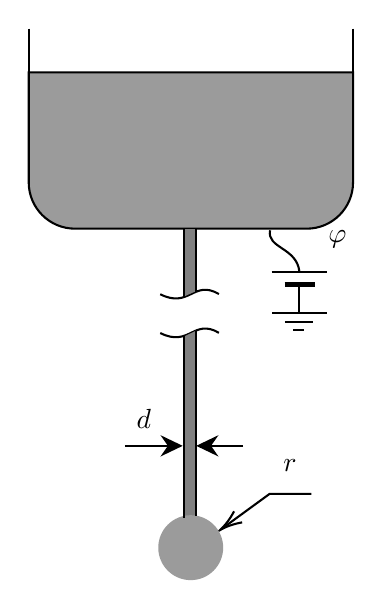
\begin{tikzpicture}[x=0.75pt,y=0.75pt,yscale=-1,xscale=1]
%uncomment if require: \path (0,481); %set diagram left start at 0, and has height of 481

%Shape: Path Data [id:dp38041072718809676] 
\draw  [fill={rgb, 255:red, 155; green, 155; blue, 155 }  ,fill opacity=1 ] (372.26,133.02) .. controls (372.26,145.35) and (362.26,155.34) .. (349.94,155.34) -- (238.32,155.34) .. controls (225.99,155.34) and (216,145.35) .. (216,133.02) -- (216,80.01) -- (372.26,80.01) -- (372.26,133.02) -- cycle ;
%Straight Lines [id:da979260137675585] 
\draw    (216,59) -- (216,80.01) ;
%Straight Lines [id:da9508250115650108] 
\draw    (372.26,59) -- (372.26,80.01) ;
%Straight Lines [id:da9336870957935353] 
\draw    (290.9,155.49) -- (290.9,188.09) ;
%Curve Lines [id:da6891291278793996] 
\draw    (279.37,186.93) .. controls (293.51,194.05) and (295.37,179.64) .. (307.65,186.84) ;
%Curve Lines [id:da20165780363618113] 
\draw    (279.37,205.61) .. controls (293.51,212.72) and (295.37,198.31) .. (307.65,205.52) ;
%Straight Lines [id:da960348632937355] 
\draw    (352.15,283.14) -- (332.02,283.14) -- (315.78,294.99) -- (309.67,299.44) ;
\draw [shift={(308.06,300.62)}, rotate = 323.89] [color={rgb, 255:red, 0; green, 0; blue, 0 }  ][line width=0.75]    (10.93,-3.29) .. controls (6.95,-1.4) and (3.31,-0.3) .. (0,0) .. controls (3.31,0.3) and (6.95,1.4) .. (10.93,3.29)   ;
%Straight Lines [id:da42993321894113445] 
\draw    (262.28,259.97) -- (287.19,259.97) ;
\draw [shift={(290.19,259.97)}, rotate = 180] [fill={rgb, 255:red, 0; green, 0; blue, 0 }  ][line width=0.08]  [draw opacity=0] (10.72,-5.15) -- (0,0) -- (10.72,5.15) -- (7.12,0) -- cycle    ;
%Straight Lines [id:da8777988841491311] 
\draw    (319.34,259.97) -- (299.72,259.97) ;
\draw [shift={(296.72,259.97)}, rotate = 360] [fill={rgb, 255:red, 0; green, 0; blue, 0 }  ][line width=0.08]  [draw opacity=0] (10.72,-5.15) -- (0,0) -- (10.72,5.15) -- (7.12,0) -- cycle    ;
%Curve Lines [id:da49129258051656444] 
\draw    (332.28,156.12) .. controls (330.55,164.88) and (345.18,164.26) .. (346.42,176.09) ;
%Straight Lines [id:da8039907925299354] 
\draw    (333.04,176.09) -- (359.81,176.09) ;
%Straight Lines [id:da6894888887093238] 
\draw [line width=1.5]    (339.26,182.26) -- (354,182.26) ;
%Straight Lines [id:da8800138646372373] 
\draw    (346.42,181.69) -- (346.42,195.91) ;
%Straight Lines [id:da03669626488440847] 
\draw    (333.27,195.91) -- (359.57,195.91) ;
%Straight Lines [id:da43999739209438515] 
\draw    (339.37,200.26) -- (352.75,200.26) ;
%Straight Lines [id:da8257723391561582] 
\draw    (343.41,204) -- (348.7,204) ;
%Shape: Rectangle [id:dp4174560488818635] 
\draw  [color={rgb, 255:red, 0; green, 0; blue, 0 }  ,draw opacity=0 ][fill={rgb, 255:red, 128; green, 128; blue, 128 }  ,fill opacity=1 ] (291.37,207.25) -- (296.15,207.25) -- (296.15,293.79) -- (291.37,293.79) -- cycle ;
%Shape: Circle [id:dp6620904343540928] 
\draw  [color={rgb, 255:red, 0; green, 0; blue, 0 }  ,draw opacity=0 ][fill={rgb, 255:red, 155; green, 155; blue, 155 }  ,fill opacity=1 ] (278.41,309.03) .. controls (278.41,300.39) and (285.41,293.38) .. (294.05,293.38) .. controls (302.69,293.38) and (309.69,300.39) .. (309.69,309.03) .. controls (309.69,317.66) and (302.69,324.67) .. (294.05,324.67) .. controls (285.41,324.67) and (278.41,317.66) .. (278.41,309.03) -- cycle ;
%Shape: Rectangle [id:dp6460372691544913] 
\draw  [color={rgb, 255:red, 0; green, 0; blue, 0 }  ,draw opacity=0 ][fill={rgb, 255:red, 128; green, 128; blue, 128 }  ,fill opacity=1 ] (291.37,155.67) -- (296.03,155.67) -- (296.03,185.74) -- (291.37,185.74) -- cycle ;
%Shape: Diagonal Stripe [id:dp48463075849565906] 
\draw  [color={rgb, 255:red, 0; green, 0; blue, 0 }  ,draw opacity=0 ][fill={rgb, 255:red, 128; green, 128; blue, 128 }  ,fill opacity=1 ] (296.43,207.35) -- (290.9,207.25) -- (296.55,204.53) -- (296.51,207.31) -- cycle ;
%Shape: Diagonal Stripe [id:dp4893234440290084] 
\draw  [color={rgb, 255:red, 0; green, 0; blue, 0 }  ,draw opacity=0 ][fill={rgb, 255:red, 128; green, 128; blue, 128 }  ,fill opacity=1 ] (291.45,185.54) -- (296.51,185.51) -- (291.39,187.74) -- (291.37,185.57) -- cycle ;
%Shape: Diagonal Stripe [id:dp5673904027318517] 
\draw  [color={rgb, 255:red, 0; green, 0; blue, 0 }  ,draw opacity=0 ][fill={rgb, 255:red, 128; green, 128; blue, 128 }  ,fill opacity=1 ] (294.18,183.85) -- (296.03,185.16) -- (291.39,187.74) -- (294.12,183.89) -- cycle ;
%Straight Lines [id:da5600211889642523] 
\draw    (296.51,155.49) -- (296.51,186.06) ;
%Straight Lines [id:da48910406449059796] 
\draw    (296.51,204.53) -- (296.51,293.83) ;
%Straight Lines [id:da9321633790876751] 
\draw    (290.9,206.56) -- (290.9,294.72) ;

% Text Node
\draw (337.2,265.14) node [anchor=north west][inner sep=0.75pt]    {$r$};
% Text Node
\draw (266.44,241.07) node [anchor=north west][inner sep=0.75pt]    {$d$};
% Text Node
\draw (358.86,154.74) node [anchor=north west][inner sep=0.75pt]    {$\varphi $};
\end{tikzpicture}
    \end{center}
    \begin{enumerate}[1)]
        \item Hãy tìm bán kính $r_{\max }$ của giọt nưóc ngay trưóc khi nó tách khỏi miệng ống.
        \item Điện thế tĩnh điện của ống so với các vật xung quanh ở rất xa là $\varphi$. Hãy tìm điện tích $Q$ của một giọt nước khi bán kính của nó là $r$.
        \item Trong câu hỏi này, giả thiết rằng $r$ được giữ không đối và $\varphi$ được tăng lên từ từ. Giọt nước trở nên không ổn định và vỡ ra thành hai mảnh nếu áp suất thủy tĩnh bên trong giọt trở nên nhỏ hơn áp suất khí quyển. Hãy tìm điện thế tới hạn $\varphi_{{\max }}$ mà ở đó điều này xảy ra.
    \end{enumerate}
    \item Hai ống\\
    Một dụng cụ, được gọi là "Ống nhỏ giọt Kelvin" gồm hai ống (giống hệt như ống đã mô tả ở Phần $\mathrm{A}$ ), được nối với nhau qua một mối nối hình chữ ${T}$, xem hình vẽ. Đầu cuối của hai ống nằm ở tâm của hai điện cực hình trụ (có độ cao $L$ và đường kính $D, L \gg D \gg r$ ); với cả hai ống, tốc độ nhỏ giọt là $n$ giọt trong một đơn vị thời gian. Các giọt nước rơi từ độ cao $H$ vào các chậu dẫn điện đặt ở dưới hai miệng ống, được mắc bắt chéo với các điện cực, như thấy trên hình; các điện cực được mắc với một tụ điện có điện dung $C$. Điện tích tổng cộng trong hệ các chậu và các điện cực bằng không. Chú ý rằng bình chứa nước được nối đất.\\
    Giọt nước đầu tiên rơi xuống mang một điện tích rất nhỏ, điện tích này gây nên sự mất cân bằng giữa hai bản của tụ điện và sự tách một lượng điện tích nhỏ giữa hai bản.
    \begin{center}
        

\tikzset{every picture/.style={line width=0.75pt}} %set default line width to 0.75pt        

\begin{tikzpicture}[x=0.75pt,y=0.75pt,yscale=-1,xscale=1]
%uncomment if require: \path (0,510); %set diagram left start at 0, and has height of 510

%Shape: Path Data [id:dp42450143317129996] 
\draw  [fill={rgb, 255:red, 155; green, 155; blue, 155 }  ,fill opacity=1 ] (389,114.42) .. controls (389,123.65) and (381.52,131.13) .. (372.29,131.13) -- (288.71,131.13) .. controls (279.48,131.13) and (272,123.65) .. (272,114.42) -- (272,74.73) -- (389,74.73) -- (389,114.42) -- cycle ;
%Straight Lines [id:da8851781572215351] 
\draw    (272,59) -- (272,74.73) ;
%Straight Lines [id:da4195462985340874] 
\draw    (389,59) -- (389,74.73) ;
%Straight Lines [id:da605998882497383] 
\draw    (327.34,131.32) -- (327.34,158) ;
%Curve Lines [id:da14920292517459854] 
\draw    (359.07,131.72) .. controls (357.77,138.28) and (368.72,137.82) .. (369.66,146.67) ;
%Straight Lines [id:da8629737388241765] 
\draw    (359.81,146.67) -- (379.5,146.67) ;
%Straight Lines [id:da7201802182966857] 
\draw    (364.37,149.8) -- (374.39,149.8) ;
%Straight Lines [id:da02448563415033389] 
\draw    (367.4,152.6) -- (371.36,152.6) ;
%Straight Lines [id:da6379873328702239] 
\draw    (332.28,130.84) -- (332.28,158) ;
%Curve Lines [id:da338533327779462] 
\draw    (244,188.52) .. controls (243.4,171.07) and (256.6,157.47) .. (268.59,158.01) ;
%Curve Lines [id:da04442258427846291] 
\draw    (416.15,188.52) .. controls (416.2,170.67) and (404.2,157.87) .. (391.56,158.01) ;
%Straight Lines [id:da6825196588989106] 
\draw    (244,188.52) -- (244,261) ;
%Straight Lines [id:da8217419592544943] 
\draw    (416.15,188.52) -- (416.15,261) ;
%Straight Lines [id:da7467371843087216] 
\draw    (268.59,158.01) -- (391.56,158.01) ;
%Curve Lines [id:da196904363482729] 
\draw    (247,192.17) .. controls (246.42,174.87) and (259.08,161.39) .. (270.57,161.93) ;
%Curve Lines [id:da06579108141887646] 
\draw    (413,192.17) .. controls (413.05,174.47) and (401.54,161.78) .. (389.43,161.93) ;
%Straight Lines [id:da8760803653733615] 
\draw    (247,192.17) -- (247,261) ;
%Straight Lines [id:da7490170370702902] 
\draw    (413,192.17) -- (413,261) ;
%Straight Lines [id:da20054774576861734] 
\draw    (270.57,161.93) -- (389.43,161.93) ;
%Straight Lines [id:da5424917424587179] 
\draw [line width=2.25]    (216,199.58) -- (216,322.42) ;
%Straight Lines [id:da7561108199821576] 
\draw [line width=2.25]    (276,199.58) -- (276,322.42) ;
%Straight Lines [id:da3119651005328443] 
\draw [line width=2.25]    (384.15,199.58) -- (384.15,322.42) ;
%Straight Lines [id:da6719017620997423] 
\draw [line width=2.25]    (443.15,199.58) -- (443.15,322.42) ;
%Straight Lines [id:da5553469383900194] 
\draw  [dash pattern={on 4.5pt off 4.5pt}]  (216,199.58) -- (276,199.58) ;
%Straight Lines [id:da2164460357829876] 
\draw  [dash pattern={on 4.5pt off 4.5pt}]  (216,322.42) -- (276,322.42) ;
%Straight Lines [id:da6101544202404989] 
\draw  [dash pattern={on 4.5pt off 4.5pt}]  (384.15,199.58) -- (444.15,199.58) ;
%Straight Lines [id:da019741114812177107] 
\draw  [dash pattern={on 4.5pt off 4.5pt}]  (384.15,322.42) -- (444.15,322.42) ;
%Shape: Path Data [id:dp619610459490628] 
\draw  [fill={rgb, 255:red, 155; green, 155; blue, 155 }  ,fill opacity=1 ] (302,416.32) .. controls (302,422.51) and (295.03,427.54) .. (286.43,427.54) -- (208.57,427.54) .. controls (199.97,427.54) and (193,422.51) .. (193,416.32) -- (193,389.67) -- (302,389.67) -- (302,416.32) -- cycle ;
%Straight Lines [id:da5256895095341783] 
\draw    (302,365.67) -- (302,389.67) ;
%Straight Lines [id:da7018381980716173] 
\draw    (193,365.67) -- (193,389.67) ;
%Shape: Path Data [id:dp23030455333276012] 
\draw  [fill={rgb, 255:red, 155; green, 155; blue, 155 }  ,fill opacity=1 ] (474,416.32) .. controls (474,422.51) and (467.03,427.54) .. (458.43,427.54) -- (380.57,427.54) .. controls (371.97,427.54) and (365,422.51) .. (365,416.32) -- (365,389.67) -- (474,389.67) -- (474,416.32) -- cycle ;
%Straight Lines [id:da6960348695075216] 
\draw    (474,365.67) -- (474,389.67) ;
%Straight Lines [id:da7604878295487274] 
\draw    (365,365.67) -- (365,389.67) ;
%Curve Lines [id:da7235996752818259] 
\draw    (276,322.42) .. controls (293,328.67) and (315,348.67) .. (365,365.67) ;
\draw [shift={(365,365.67)}, rotate = 18.78] [color={rgb, 255:red, 0; green, 0; blue, 0 }  ][fill={rgb, 255:red, 0; green, 0; blue, 0 }  ][line width=0.75]      (0, 0) circle [x radius= 2.01, y radius= 2.01]   ;
\draw [shift={(276,322.42)}, rotate = 20.18] [color={rgb, 255:red, 0; green, 0; blue, 0 }  ][fill={rgb, 255:red, 0; green, 0; blue, 0 }  ][line width=0.75]      (0, 0) circle [x radius= 2.01, y radius= 2.01]   ;
%Shape: Arc [id:dp03104125885768405] 
\draw  [draw opacity=0] (337.35,347.2) .. controls (337.96,347.74) and (338.48,348.39) .. (338.89,349.14) .. controls (340.77,352.61) and (339.48,356.94) .. (336.01,358.82) .. controls (332.54,360.7) and (328.21,359.41) .. (326.33,355.94) .. controls (325.92,355.18) and (325.67,354.39) .. (325.55,353.59) -- (332.61,352.54) -- cycle ; \draw   (337.35,347.2) .. controls (337.96,347.74) and (338.48,348.39) .. (338.89,349.14) .. controls (340.77,352.61) and (339.48,356.94) .. (336.01,358.82) .. controls (332.54,360.7) and (328.21,359.41) .. (326.33,355.94) .. controls (325.92,355.18) and (325.67,354.39) .. (325.55,353.59) ;
%Curve Lines [id:da13879854521724977] 
\draw    (337.35,347.2) .. controls (362.83,333.92) and (389.89,316.44) .. (384.15,322.42) ;
\draw [shift={(384.15,322.42)}, rotate = 133.85] [color={rgb, 255:red, 0; green, 0; blue, 0 }  ][fill={rgb, 255:red, 0; green, 0; blue, 0 }  ][line width=0.75]      (0, 0) circle [x radius= 2.01, y radius= 2.01]   ;
%Curve Lines [id:da8849865810804174] 
\draw    (302,365.67) .. controls (327.48,352.38) and (314.47,358.93) .. (325.55,353.59) ;
\draw [shift={(302,365.67)}, rotate = 332.47] [color={rgb, 255:red, 0; green, 0; blue, 0 }  ][fill={rgb, 255:red, 0; green, 0; blue, 0 }  ][line width=0.75]      (0, 0) circle [x radius= 2.01, y radius= 2.01]   ;
%Curve Lines [id:da5211199320904487] 
\draw    (276.52,223.81) .. controls (288.19,226.5) and (301.29,227.49) .. (318.29,227.67) ;
\draw [shift={(276.52,223.81)}, rotate = 13] [color={rgb, 255:red, 0; green, 0; blue, 0 }  ][fill={rgb, 255:red, 0; green, 0; blue, 0 }  ][line width=0.75]      (0, 0) circle [x radius= 2.01, y radius= 2.01]   ;
%Shape: Contact [id:dp11839770990052623] 
\draw  [line width=2.25]  (318.29,227.67) -- (325.99,227.67) (343.95,227.67) -- (336.25,227.67) (325.99,218.05) -- (325.99,237.3) (336.25,218.05) -- (336.25,237.3) ;
%Curve Lines [id:da7037249551592384] 
\draw    (343.95,227.67) .. controls (354.47,228) and (371.27,226) .. (384.47,224.4) ;
\draw [shift={(384.47,224.4)}, rotate = 353.09] [color={rgb, 255:red, 0; green, 0; blue, 0 }  ][fill={rgb, 255:red, 0; green, 0; blue, 0 }  ][line width=0.75]      (0, 0) circle [x radius= 2.01, y radius= 2.01]   ;
%Straight Lines [id:da7842014146043463] 
\draw    (226,221.97) -- (240.19,221.97) ;
\draw [shift={(243.19,221.97)}, rotate = 180] [fill={rgb, 255:red, 0; green, 0; blue, 0 }  ][line width=0.08]  [draw opacity=0] (10.72,-5.15) -- (0,0) -- (10.72,5.15) -- (7.12,0) -- cycle    ;
%Straight Lines [id:da17191387347745546] 
\draw    (263,221.97) -- (250.19,221.97) ;
\draw [shift={(247.19,221.97)}, rotate = 360] [fill={rgb, 255:red, 0; green, 0; blue, 0 }  ][line width=0.08]  [draw opacity=0] (10.72,-5.15) -- (0,0) -- (10.72,5.15) -- (7.12,0) -- cycle    ;
%Straight Lines [id:da9157719417444774] 
\draw    (200,261) -- (235.2,261) ;
%Straight Lines [id:da9700031127005864] 
\draw    (200,264) -- (200,386) ;
\draw [shift={(200,389)}, rotate = 270] [fill={rgb, 255:red, 0; green, 0; blue, 0 }  ][line width=0.08]  [draw opacity=0] (10.72,-5.15) -- (0,0) -- (10.72,5.15) -- (7.12,0) -- cycle    ;
\draw [shift={(200,261)}, rotate = 90] [fill={rgb, 255:red, 0; green, 0; blue, 0 }  ][line width=0.08]  [draw opacity=0] (10.72,-5.15) -- (0,0) -- (10.72,5.15) -- (7.12,0) -- cycle    ;
%Straight Lines [id:da7473425562457661] 
\draw    (440.15,301.42) -- (387.15,301.42) ;
\draw [shift={(384.15,301.42)}, rotate = 360] [fill={rgb, 255:red, 0; green, 0; blue, 0 }  ][line width=0.08]  [draw opacity=0] (10.72,-5.15) -- (0,0) -- (10.72,5.15) -- (7.12,0) -- cycle    ;
\draw [shift={(443.15,301.42)}, rotate = 180] [fill={rgb, 255:red, 0; green, 0; blue, 0 }  ][line width=0.08]  [draw opacity=0] (10.72,-5.15) -- (0,0) -- (10.72,5.15) -- (7.12,0) -- cycle    ;
%Straight Lines [id:da5567744893942874] 
\draw    (443.15,199.58) -- (468,199.58) ;
%Straight Lines [id:da4656694571611153] 
\draw    (443.15,322.42) -- (468,322.42) ;
%Straight Lines [id:da8278754881137489] 
\draw    (455.58,202.58) -- (455.58,319.42) ;
\draw [shift={(455.58,322.42)}, rotate = 270] [fill={rgb, 255:red, 0; green, 0; blue, 0 }  ][line width=0.08]  [draw opacity=0] (10.72,-5.15) -- (0,0) -- (10.72,5.15) -- (7.12,0) -- cycle    ;
\draw [shift={(455.58,199.58)}, rotate = 90] [fill={rgb, 255:red, 0; green, 0; blue, 0 }  ][line width=0.08]  [draw opacity=0] (10.72,-5.15) -- (0,0) -- (10.72,5.15) -- (7.12,0) -- cycle    ;
%Shape: Polygon Curved [id:ds11788841734154176] 
\draw  [fill={rgb, 255:red, 128; green, 128; blue, 128 }  ,fill opacity=1 ] (268.59,158.01) .. controls (273.84,157.52) and (379,158.21) .. (391.56,158.01) .. controls (407,158.96) and (416,172.96) .. (416.15,188.52) .. controls (416.25,199.54) and (416.25,232.04) .. (416.25,249.54) .. controls (415,260.49) and (417.77,258.33) .. (413.13,250.5) .. controls (412.93,231.23) and (412.93,219.03) .. (413,192.17) .. controls (412.53,167.43) and (395.33,162.03) .. (389.43,161.93) .. controls (359.2,161.83) and (303.6,162.03) .. (270.57,161.93) .. controls (254,163.23) and (247,178.03) .. (247,192.17) .. controls (247.2,218.3) and (247,220.88) .. (247.25,249.88) .. controls (242.13,260.03) and (248.44,259.41) .. (244.25,249.96) .. controls (244.25,209.54) and (244.25,207.29) .. (244,188.52) .. controls (243,171.46) and (256.25,160.21) .. (262.67,158.5) .. controls (265,158.17) and (265.17,158.17) .. (265.41,158.19) .. controls (265.53,158.2) and (265.67,158.22) .. (266.1,158.2) .. controls (266.32,158.19) and (266.61,158.17) .. (267.02,158.14) .. controls (267.22,158.13) and (267.45,158.11) .. (267.71,158.09) .. controls (267.84,158.08) and (267.98,158.07) .. (268.12,158.05) .. controls (268.2,158.05) and (268.27,158.04) .. (268.35,158.03) .. controls (268.39,158.03) and (268.43,158.03) .. (268.47,158.02) .. controls (268.49,158.02) and (268.51,158.02) .. (268.53,158.02) .. controls (268.54,158.02) and (268.55,158.01) .. (268.56,158.01) .. controls (268.57,158.01) and (268.58,158.01) .. (268.59,158.01) -- cycle ;
%Shape: Circle [id:dp4465313406784768] 
\draw  [color={rgb, 255:red, 0; green, 0; blue, 0 }  ,draw opacity=0 ][fill={rgb, 255:red, 155; green, 155; blue, 155 }  ,fill opacity=1 ] (403.36,261) .. controls (403.36,255.04) and (408.19,250.2) .. (414.15,250.2) .. controls (420.11,250.2) and (424.95,255.04) .. (424.95,261) .. controls (424.95,266.96) and (420.11,271.8) .. (414.15,271.8) .. controls (408.19,271.8) and (403.36,266.96) .. (403.36,261) -- cycle ;
%Shape: Circle [id:dp37636809259094317] 
\draw  [color={rgb, 255:red, 0; green, 0; blue, 0 }  ,draw opacity=0 ][fill={rgb, 255:red, 155; green, 155; blue, 155 }  ,fill opacity=1 ] (235.2,261) .. controls (235.2,255.04) and (240.04,250.2) .. (246,250.2) .. controls (251.96,250.2) and (256.79,255.04) .. (256.79,261) .. controls (256.79,266.96) and (251.96,271.8) .. (246,271.8) .. controls (240.04,271.8) and (235.2,266.96) .. (235.2,261) -- cycle ;
%Shape: Rectangle [id:dp33663081014716334] 
\draw  [color={rgb, 255:red, 0; green, 0; blue, 0 }  ,draw opacity=0 ][fill={rgb, 255:red, 128; green, 128; blue, 128 }  ,fill opacity=1 ] (327.75,131.48) -- (331.89,131.48) -- (331.89,160.25) -- (327.75,160.25) -- cycle ;

% Text Node
\draw (325.47,197.4) node [anchor=north west][inner sep=0.75pt]    {$C$};
% Text Node
\draw (229.44,202.07) node [anchor=north west][inner sep=0.75pt]    {$d$};
% Text Node
\draw (180,316.4) node [anchor=north west][inner sep=0.75pt]    {$H$};
% Text Node
\draw (406,283.4) node [anchor=north west][inner sep=0.75pt]    {$D$};
% Text Node
\draw (460,252.4) node [anchor=north west][inner sep=0.75pt]    {$L$};
% Text Node
\draw (360,321) node [anchor=north west][inner sep=0.75pt]  [rotate=-270] [align=left] {Điện cực hình trụ};
\end{tikzpicture}
    \end{center}
    \begin{enumerate}[1)]
        \item Hãy biểu thị giá trị tuyệt đối của điện tích $Q_{0}$ của các giọt nước tách ra vào lúc mà điện tích của tụ điện là $q$, theo $r_{\max }$ (từ Phần A-1). Bỏ qua hiệu ứng đã được mô tả ở Phần A-3.
        \item Hãy tìm sự phụ thuộc của $q$ vào thời gian $t$ bằng cách làm gần đúng nó bằng một hàm liên tục $q(t)$ và giả thiết rằng $q(0)=q_{0}$.
        \item Hoạt động của ống nhỏ giọt có thể bị cản trở bởi hiệu ứng đã nêu ở Phần A-3. Thêm vào đó, có một giới hạn $U_{\max}$ cho điện áp có thể đạt được giữa các điện cực, điện áp này được xác lập bởi lực đẩy tĩnh điện giữa một giọt và chậu ở phía dưới nó; hãy tìm $U_{\max }$.
    \end{enumerate}
\end{enumerate}
\end{vd}
\begin{loigiai}\[\]
\begin{enumerate}[\bf Phần A.]
    \item 
    \begin{enumerate}[1)]
        \item Hãy viết cân bằng lực cho giọt nước. Vì $d \ll r$, chúng ta có thể bỏ qua lực $\dfrac{\pi}{4} \Delta p d^2$ do áp suất phụ $\Delta p$ bên trong ống. Vì vậy, lực hấp dẫn $\dfrac{4}{3} \pi r_{\max }^{3}\rho g$ được cân bởi lực mao dẫn (lực căng mặt ngoài). Khi giọt nước rời khỏi ống, mặt nước tạo trong vùng lân cận của vòi một "cổ", có tiếp tuyến thẳng đứng. Trong mặt cắt ngang của "cổ" đó, lực mao dẫn có phương thẳng đứng và có thể được tính bởi $\pi \sigma d$. Vì thế:
        \[r_{\max }=\sqrt[3]{\dfrac{3 \sigma d}{4 \rho g}}.\]
        \item Vì $d \ll r$ nên ta có thể bỏ qua sự thay đổi của điện dung của giọt nước do ống. Điện thế của giọt $\varphi$ bằng $\dfrac{1}{4 \pi \varepsilon_{0}} \dfrac{Q}{r}$. Vì vậy
        \[Q = 4 \pi \varepsilon_{0} \varphi r.\]
        \item Áp suất phụ bên trong giọt nước là do áp suất mao dẫn $ \dfrac{2 \sigma}{r}$ (tăng áp suất bên trong), và bởi áp suất tĩnh điện $\dfrac{1}{2} \varepsilon_{0} E^{2} = \dfrac{1}{2} \varepsilon_{0} \dfrac{\varphi^{2}}{r^{2}}$ (giảm áp suất bên trong). Vì vậy, dấu của áp suất phụ sẽ thay đổi, nếu $\dfrac{1}{2} \varepsilon_{0} \dfrac{\varphi_{\max}^{2}}{r^{2}}=\dfrac{2 \sigma}{r}$, do đó:
        \[\varphi_{\max }=2 \sqrt{\dfrac{\sigma r}{\varepsilon_{0}}}.\]
        Biểu thức cho áp suất tĩnh điện được sử dụng ở trên có thể được suy ra như sau. Lực tĩnh điện tác dụng lên một bề mặt có diện tích ${S}$ và có mật độ điện tích mặt $\sigma$ được cho bởi biểu thức $F=\sigma S \overline{E}$, trong đó $\overline{E}$ là điện trường tại vị trí mà không có điện trường được tạo bởi chính yếu tố điện tích bề mặt đó. Lưu ý rằng, lực này vuông góc với bề mặt, vì vậy $\dfrac{F}{S}$ có thể được hiểu là một áp suất.\\
        Điện tích trên bề mặt gây ra một điện trường tại điểm ở sát bề mặt có độ lớn bằng $\Delta E = \dfrac{\sigma}{\varepsilon_0}$ (theo định luật Gauss) làm giảm điện trường ở bên ngoài; bên trong giọt nước, không có trường do  tính dẫn điện của nước: $\overline{E} - \dfrac{1}{2}\Delta E = 0$; bên ngoài giọt nước, có trường $E = \overline{E} + \dfrac{1}{2}\Delta  E$, do đó $\overline{E} = \dfrac{1}{2}E = \dfrac{1}{2}\Delta E$. Kết hợp mọi thứ lại với nhau, chúng ta có được biểu thức được sử dụng ở trên.\\
        \textbf{Lưu ý.} Biểu thức này có thể được suy ra bằng cách xét một sự dịch chuyển ảo của bề mặt tụ điện và so sánh với công của áp suất $p \Delta V$ với thay đổi của năng lượng trường tĩnh điện.
        \[\dfrac{1}{2} \varepsilon_{0} E^{2} \Delta V.\]
        Cuối cùng, câu trả lời cho câu hỏi cũng có thể được bắt nguồn từ yêu cầu rằng công cơ học $\dd A$ sinh ra khi làm giãn nở một giọt rất nhỏ cần phải bằng không. Từ định luật bảo toàn năng lượng,
        \[\dd W + \dd W_\text{el}= \sigma \dd\left(4 \pi r^{2}\right) + \dfrac{1}{2} \varphi_{\max }^{2} \dd C_{d},\]
        ở đây điện dung của giọt nước là $C_{{d}}=4 \pi \varepsilon_{0} r$, và công của lực điện
        \[\dd W_\text{el}=\varphi_{\max} \dd q = 4 \pi \varepsilon_{0} \varphi_{\max }^{2} \dd r.\]
        Cho $\dd W=0$ ta thu được phương trình cho $\varphi_{\max }$, từ đó ta thu được kết quả trước đó.
    \end{enumerate}
    \item 
    \begin{enumerate}[1)]
        \item Về cơ bản giống như Phần A-2, ngoại trừ điện thế xung quanh là điện thế của các điện cực xung quanh, $-\dfrac{U}{2}$ (trong đó $U = \dfrac{q}{C}$ là điện áp của tụ điện) và giọt nước có điện thế mặt đất ($0$). Vì không xác định được điện cực nào là điện cực dương, nên dấu của điện thế có thể được chọn ngược lại, nếu được thực hiện một cách nhất quán. Lưu ý rằng vì điện cực có dạng hình trụ dài, nó là lá chắn hiệu quả điện thế của môi trường (mặt đất, tường,...). Vì vậy, so với môi trường xung quanh, điện thế của giọt nước là  $\dfrac{U}{2}$. Sử dụng kết quả của Phần $A$ chúng ta có được:
        \[Q=2 \pi \varepsilon_{0} U r_{\max}=2 \pi \varepsilon_{0} r_{\max } \dfrac{q}{C}.\]
        \item  Dấu của giọt điện tích giống với dấu  của bản tụ đối diện (được nối với điện cực xa hơn). Vì vậy, khi giọt nước rơi vào chậu, nó sẽ làm tăng điện tích của chậu một lượng là $Q$:
        \[\dd q = 2\pi \varepsilon_0 U r_{\max} \dd N =  2\pi \varepsilon_0 v n \dd t  \dfrac{q}{C},\]
        trong đó $\dd N = n \dd t$ là số giọt rơi xuống trong thời gian $\dd t$. Đây là phương trình vi phân tuyến tính đơn giản, ta dễ dàng giải và thu được kết quả:
        \[ q=q_{0} e^{\gamma t}, \quad \gamma = \dfrac{2 \pi \varepsilon_{0} r_{\max} n}{C} = \dfrac{\pi \varepsilon_{0} n}{C} \sqrt[3]{\dfrac{6 \sigma d}{\rho g}}.\]
        \item Các giọt nước có thể chạm tới các chậu nếu năng lượng cơ học của chúng ${mgH}$ (trong đó ${m}$ là khối lượng của giọt nước) đủ lớn để vượt qua lực đẩy tĩnh điện. Các giọt bắt đầu tại điểm mà điện thế là $0$, là tổng của điện thế $\dfrac{U}{2}$ do điện cực, và điện thế tự tạo ra của nó $-\dfrac{U}{2}$. Chuyển động của nó không bị ảnh hưởng bởi trường tự tạo ra, do đó, nó cần phải rơi từ điện thế $\dfrac{U}{2}$ xuống điện thế $-\dfrac{U}{2}$, dẫn đến sự thay đổi năng lượng tĩnh điện bằng $U Q \leq m g H$, trong đó $Q=2 \pi \varepsilon_{0} U r_{\max }$ (xem ở trên). Vì thế,
        \[U_{\max} = \dfrac{mgH}{2\pi \varepsilon_0 U_{\max} r_{\max}},\]
        \[\rt U_{\max} = \sqrt{\dfrac{H\sigma d}{2\varepsilon_0 r_{\max}}} = \sqrt[6]{\dfrac{H^3 g \sigma^2 \rho d^2}{6\varepsilon_0^3}}.\]
    \end{enumerate}
\end{enumerate}
\end{loigiai}


\begin{vd}[Túi khí] %IPhO 2007
Trong bài này chúng ta xét mô hình đơn giản hóa của một gia tốc kế dùng để kích hoạt các túi khí an toàn trong các ô tô khi xảy ra va chạm. Chúng ta muốn xây dựng một hệ cơ điện sao cho khi gia tốc vượt quá một giới hạn nhất định thì một trong những thông số điện của hệ thống, chẳng hạn như điện thế ở một điểm nhất định nào đó của mạch điện sẽ vượt quá ngưỡng và kết quả là túi khí sẽ bị kích hoạt.\\
\textbf{Chú thích.} Bỏ qua trọng lực trong bài toán này.
\begin{enumerate}[1)]
    \item Xét một tụ điện có các bản song song như trên Hình $1$. Diện tích của mỗi bản tụ điện là $A$ và khoảng cách giữa hai bản là $d$. Khoảng cách giữa hai bản rất nhỏ so với kích thước của các bản. Một trong các bản này gắn với tường bởi một lò xo có độ cứng $k$, và bản còn lại được giữ cố định. Khi khoảng cách giữa các bản là $d$ thì lò xo không bị nén cũng như không bị dãn, nói cách khác, không có lực nào xuất hiện trong lò xo ở trạng thái này. Giả thiết rằng độ điện thẩm của không khí giữa các bản bằng độ điện thẩm của chân không $\varepsilon_{0}$. Điện dung tương ứng với khoảng cách này giữa các bản tụ điện là $C_{0} = \dfrac{\varepsilon_{0} A }{d}$. Ta nạp điện tích $+Q$ và $-Q$ vào các bản và để hệ thống đạt trạng thái cân bằng cơ học.
    \begin{center}
    

\tikzset{every picture/.style={line width=0.75pt}} %set default line width to 0.75pt        

\begin{tikzpicture}[x=0.75pt,y=0.75pt,yscale=-1,xscale=1]
%uncomment if require: \path (0,504); %set diagram left start at 0, and has height of 504

%Straight Lines [id:da4078078527754736] 
\draw    (221,181) -- (284.67,181) ;
%Straight Lines [id:da33020380433553953] 
\draw    (284.67,115.63) -- (284.67,246.38) ;
%Straight Lines [id:da470619580645242] 
\draw    (369.67,115.63) -- (369.67,246.38) ;
%Shape: Spring [id:dp971528578457076] 
\draw   (369.93,182.2) .. controls (371.17,177.44) and (374.38,172.69) .. (380.81,172.69) .. controls (393.65,172.69) and (393.65,191.71) .. (390.69,191.71) .. controls (387.72,191.71) and (387.72,172.69) .. (400.57,172.69) .. controls (413.42,172.69) and (413.42,191.71) .. (410.46,191.71) .. controls (407.49,191.71) and (407.49,172.69) .. (420.34,172.69) .. controls (433.19,172.69) and (433.19,191.71) .. (430.22,191.71) .. controls (427.26,191.71) and (427.26,172.69) .. (440.11,172.69) .. controls (452.95,172.69) and (452.95,191.71) .. (449.99,191.71) .. controls (447.02,191.71) and (447.02,172.69) .. (459.87,172.69) .. controls (465.66,172.69) and (468.84,176.55) .. (470.32,180.8) ;
%Straight Lines [id:da16366822956322924] 
\draw    (470.5,96.25) -- (470.5,268.83) ;
%Straight Lines [id:da01501965660468585] 
\draw    (470.5,96.25) -- (482.91,83.83) ;
%Straight Lines [id:da3775024785484553] 
\draw    (470.5,268.83) -- (482.91,256.42) ;
%Straight Lines [id:da20108059353196794] 
\draw    (470.5,182.54) -- (482.91,170.13) ;
%Straight Lines [id:da15742694506344024] 
\draw    (470.35,127.73) -- (482.76,115.32) ;
%Straight Lines [id:da20122683633239236] 
\draw    (470.62,155.16) -- (483.03,142.75) ;
%Straight Lines [id:da3221890761363029] 
\draw    (470.5,209.92) -- (482.91,197.51) ;
%Straight Lines [id:da8839894786534996] 
\draw    (470.5,237.17) -- (482.91,224.76) ;
%Straight Lines [id:da41255172104265436] 
\draw    (287.67,263.38) -- (366.67,263.38) ;
\draw [shift={(369.67,263.38)}, rotate = 180] [fill={rgb, 255:red, 0; green, 0; blue, 0 }  ][line width=0.08]  [draw opacity=0] (10.72,-5.15) -- (0,0) -- (10.72,5.15) -- (7.12,0) -- cycle    ;
\draw [shift={(284.67,263.38)}, rotate = 0] [fill={rgb, 255:red, 0; green, 0; blue, 0 }  ][line width=0.08]  [draw opacity=0] (10.72,-5.15) -- (0,0) -- (10.72,5.15) -- (7.12,0) -- cycle    ;

% Text Node
\draw (321.17,268.77) node [anchor=north west][inner sep=0.75pt]    {$d$};
% Text Node
\draw (420,155.4) node [anchor=north west][inner sep=0.75pt]    {$k$};
\end{tikzpicture}\\ Hình $1$.
    \end{center}
    \begin{enumerate}[a)]
        \item Hãy tính lực điện $F_{E}$ mà các bản tác dụng lên nhau.
        \item Gọi $x$ là độ dịch của bản nối với lò xo. Hãy tìm $x$.
        \item Ở trạng thái này, hãy tìm hiệu điện thế $V$ giữa các bản tụ điện theo $Q, A, d, k$.
        \item Gọi $C$ là điện dung của tụ điện, được định nghĩa là tỉ số của điện tích với hiệu điện thế. Hãy tìm $ \dfrac{C}{C_0}$ theo $Q, A, d$ và $k$.
        \item Tìm năng lượng toàn phần $U$ dự trữ trong hệ thống theo $Q, A, d$ và $k$.
    \end{enumerate}
    \end{enumerate}
    Hình $2$ trình bày một vật khối lượng $M$ gắn với một bản dẫn điện có khối lượng không đáng kể. Vật đó cũng được gắn với hai lò xo có cùng độ cứng $k$. Bản dẫn điện này (gọi là bản di động) có thể dịch chuyển trong khoảng giữa hai bản dẫn điện cố định. Tất cả các bản đều giống nhau và có cùng diện tích $A$. Như vậy, ba bản này tạo thành hai tụ điện. Như trình bày trên Hình $2$, các bản cố định được nối với các điện thế cho trước $V$ và $-V$, còn bản ở giữa thì nối đất thông qua một cái chuyển mạch hai trạng thái. Dây dẫn nối với bản di động không làm ảnh hưởng đến chuyển động của bản và ba bản này luôn luôn song song với nhau. Khi toàn bộ hệ thống không có gia tốc thì khoảng cách giữa mỗi bản cố định và bản di động là $d$, nhỏ hơn rất nhiều so với kích thước của các bản. Độ dày của các bản có thể bỏ qua.
    \begin{center}
        

% Pattern Info
 
\tikzset{
pattern size/.store in=\mcSize, 
pattern size = 5pt,
pattern thickness/.store in=\mcThickness, 
pattern thickness = 0.3pt,
pattern radius/.store in=\mcRadius, 
pattern radius = 1pt}
\makeatletter
\pgfutil@ifundefined{pgf@pattern@name@_nxjf0hm4p}{
\makeatletter
\pgfdeclarepatternformonly[\mcRadius,\mcThickness,\mcSize]{_nxjf0hm4p}
{\pgfpoint{-0.5*\mcSize}{-0.5*\mcSize}}
{\pgfpoint{0.5*\mcSize}{0.5*\mcSize}}
{\pgfpoint{\mcSize}{\mcSize}}
{
\pgfsetcolor{\tikz@pattern@color}
\pgfsetlinewidth{\mcThickness}
\pgfpathcircle\pgfpointorigin{\mcRadius}
\pgfusepath{stroke}
}}
\makeatother
\tikzset{every picture/.style={line width=0.75pt}} %set default line width to 0.75pt        

\begin{tikzpicture}[x=0.75pt,y=0.75pt,yscale=-1,xscale=1]
%uncomment if require: \path (0,645); %set diagram left start at 0, and has height of 645

%Flowchart: Process [id:dp9361072921990328] 
\draw  [line width=3]  (270,65) -- (421.67,65) -- (421.67,207.5) -- (270,207.5) -- cycle ;
%Shape: Rectangle [id:dp678216249227884] 
\draw  [color={rgb, 255:red, 0; green, 0; blue, 0 }  ,draw opacity=1 ][fill={rgb, 255:red, 0; green, 0; blue, 0 }  ,fill opacity=1 ] (301.5,117.42) -- (306.5,117.42) -- (306.5,207.92) -- (301.5,207.92) -- cycle ;
%Shape: Rectangle [id:dp3833196180860883] 
\draw  [color={rgb, 255:red, 0; green, 0; blue, 0 }  ,draw opacity=1 ][fill={rgb, 255:red, 0; green, 0; blue, 0 }  ,fill opacity=1 ] (343.5,117.42) -- (348.5,117.42) -- (348.5,207.92) -- (343.5,207.92) -- cycle ;
%Shape: Rectangle [id:dp5311323292842491] 
\draw  [color={rgb, 255:red, 0; green, 0; blue, 0 }  ,draw opacity=1 ][fill={rgb, 255:red, 0; green, 0; blue, 0 }  ,fill opacity=1 ] (385.5,117.42) -- (390.5,117.42) -- (390.5,207.92) -- (385.5,207.92) -- cycle ;
%Shape: Spring [id:dp9326877077286746] 
\draw   (269.5,100.96) .. controls (269.75,97.65) and (270.75,94.33) .. (272.75,94.33) .. controls (276.75,94.33) and (276.75,107.58) .. (274.75,107.58) .. controls (272.75,107.58) and (272.75,94.33) .. (276.75,94.33) .. controls (280.75,94.33) and (280.75,107.58) .. (278.75,107.58) .. controls (276.75,107.58) and (276.75,94.33) .. (280.75,94.33) .. controls (284.75,94.33) and (284.75,107.58) .. (282.75,107.58) .. controls (280.75,107.58) and (280.75,94.33) .. (284.75,94.33) .. controls (288.75,94.33) and (288.75,107.58) .. (286.75,107.58) .. controls (284.75,107.58) and (284.75,94.33) .. (288.75,94.33) .. controls (292.75,94.33) and (292.75,107.58) .. (290.75,107.58) .. controls (288.75,107.58) and (288.75,94.33) .. (292.75,94.33) .. controls (296.75,94.33) and (296.75,107.58) .. (294.75,107.58) .. controls (292.75,107.58) and (292.75,94.33) .. (296.75,94.33) .. controls (300.75,94.33) and (300.75,107.58) .. (298.75,107.58) .. controls (296.75,107.58) and (296.75,94.33) .. (300.75,94.33) .. controls (304.75,94.33) and (304.75,107.58) .. (302.75,107.58) .. controls (300.75,107.58) and (300.75,94.33) .. (304.75,94.33) .. controls (308.75,94.33) and (308.75,107.58) .. (306.75,107.58) .. controls (304.75,107.58) and (304.75,94.33) .. (308.75,94.33) .. controls (312.75,94.33) and (312.75,107.58) .. (310.75,107.58) .. controls (308.75,107.58) and (308.75,94.33) .. (312.75,94.33) .. controls (313.22,94.33) and (313.64,94.52) .. (314,94.84) ;
%Flowchart: Process [id:dp363389129882153] 
\draw  [pattern=_nxjf0hm4p,pattern size=0.75pt,pattern thickness=0.75pt,pattern radius=0.75pt, pattern color={rgb, 255:red, 0; green, 0; blue, 0}][line width=3]  (315.5,86.08) -- (376,86.08) -- (376,116.08) -- (315.5,116.08) -- cycle ;
%Shape: Spring [id:dp3124009056316599] 
\draw   (377,100.46) .. controls (377.25,97.15) and (378.25,93.83) .. (380.25,93.83) .. controls (384.25,93.83) and (384.25,107.08) .. (382.25,107.08) .. controls (380.25,107.08) and (380.25,93.83) .. (384.25,93.83) .. controls (388.25,93.83) and (388.25,107.08) .. (386.25,107.08) .. controls (384.25,107.08) and (384.25,93.83) .. (388.25,93.83) .. controls (392.25,93.83) and (392.25,107.08) .. (390.25,107.08) .. controls (388.25,107.08) and (388.25,93.83) .. (392.25,93.83) .. controls (396.25,93.83) and (396.25,107.08) .. (394.25,107.08) .. controls (392.25,107.08) and (392.25,93.83) .. (396.25,93.83) .. controls (400.25,93.83) and (400.25,107.08) .. (398.25,107.08) .. controls (396.25,107.08) and (396.25,93.83) .. (400.25,93.83) .. controls (404.25,93.83) and (404.25,107.08) .. (402.25,107.08) .. controls (400.25,107.08) and (400.25,93.83) .. (404.25,93.83) .. controls (408.25,93.83) and (408.25,107.08) .. (406.25,107.08) .. controls (404.25,107.08) and (404.25,93.83) .. (408.25,93.83) .. controls (412.25,93.83) and (412.25,107.08) .. (410.25,107.08) .. controls (408.25,107.08) and (408.25,93.83) .. (412.25,93.83) .. controls (416.25,93.83) and (416.25,107.08) .. (414.25,107.08) .. controls (412.25,107.08) and (412.25,93.83) .. (416.25,93.83) .. controls (420.25,93.83) and (420.25,107.08) .. (418.25,107.08) .. controls (416.25,107.08) and (416.25,93.83) .. (420.25,93.83) .. controls (420.72,93.83) and (421.14,94.02) .. (421.5,94.34) ;
%Straight Lines [id:da3835283048207645] 
\draw    (451,87.67) -- (516,87.67) ;
\draw [shift={(519,87.67)}, rotate = 180] [fill={rgb, 255:red, 0; green, 0; blue, 0 }  ][line width=0.08]  [draw opacity=0] (10.72,-5.15) -- (0,0) -- (10.72,5.15) -- (7.12,0) -- cycle    ;
%Straight Lines [id:da08567129540443297] 
\draw  [dash pattern={on 4.5pt off 4.5pt}]  (304,162.67) -- (227.84,136.64) ;
\draw [shift={(225,135.67)}, rotate = 378.87] [fill={rgb, 255:red, 0; green, 0; blue, 0 }  ][line width=0.08]  [draw opacity=0] (10.72,-5.15) -- (0,0) -- (10.72,5.15) -- (7.12,0) -- cycle    ;
%Straight Lines [id:da7777756485484231] 
\draw  [dash pattern={on 4.5pt off 4.5pt}]  (346,162.67) -- (453.09,189.93) ;
\draw [shift={(456,190.67)}, rotate = 194.28] [fill={rgb, 255:red, 0; green, 0; blue, 0 }  ][line width=0.08]  [draw opacity=0] (10.72,-5.15) -- (0,0) -- (10.72,5.15) -- (7.12,0) -- cycle    ;
%Straight Lines [id:da18137330979689503] 
\draw  [dash pattern={on 4.5pt off 4.5pt}]  (388,162.67) -- (455.2,136.75) ;
\draw [shift={(458,135.67)}, rotate = 518.9100000000001] [fill={rgb, 255:red, 0; green, 0; blue, 0 }  ][line width=0.08]  [draw opacity=0] (10.72,-5.15) -- (0,0) -- (10.72,5.15) -- (7.12,0) -- cycle    ;
%Straight Lines [id:da05669685539945046] 
\draw [line width=1.5]    (373.89,314.88) -- (393.67,314.88) ;
%Straight Lines [id:da14028819679317484] 
\draw [line width=1.5]    (376.89,317.88) -- (391.19,317.88) ;
%Straight Lines [id:da036001937633450165] 
\draw [line width=1.5]    (379.88,320.87) -- (387.28,320.87) ;
%Straight Lines [id:da5643344794637897] 
\draw [line width=1.5]    (383.78,306.44) -- (383.78,314.88) ;
%Straight Lines [id:da42714708102841636] 
\draw [line width=1.5]    (264,255.67) -- (264,274.67) ;
%Straight Lines [id:da4832986651657398] 
\draw [line width=1.5]    (247.88,274.67) -- (280.13,274.67) ;
%Straight Lines [id:da23302727576769144] 
\draw [line width=1.5]    (259.88,279.67) -- (267.5,279.67) ;
%Straight Lines [id:da5333285739640938] 
\draw [line width=1.5]    (264,279.67) -- (264,306.75) ;
%Straight Lines [id:da2906958439654783] 
\draw [line width=1.5]    (264,306.75) -- (412.5,306.75) ;
%Straight Lines [id:da7010042363184581] 
\draw [line width=1.5]    (412,255.67) -- (412,274.67) ;
%Straight Lines [id:da420339840247002] 
\draw [line width=1.5]    (395.88,279.67) -- (428.13,279.67) ;
%Straight Lines [id:da4710928948907174] 
\draw [line width=1.5]    (408.38,274.67) -- (416,274.67) ;
%Straight Lines [id:da01566268084683542] 
\draw [line width=1.5]    (412,279.67) -- (412,306.75) ;
%Straight Lines [id:da6088299736356777] 
\draw [line width=1.5]    (309,274.42) -- (309,306.67) ;
%Straight Lines [id:da39776679769460577] 
\draw [line width=1.5]    (309,274.42) -- (318.02,274.42) ;
\draw [shift={(320.5,274.42)}, rotate = 0] [color={rgb, 255:red, 0; green, 0; blue, 0 }  ][line width=1.5]      (0, 0) circle [x radius= 3.48, y radius= 3.48]   ;
%Straight Lines [id:da9885210946157079] 
\draw [line width=1.5]    (359,274.42) -- (348.98,274.42) ;
\draw [shift={(346.5,274.42)}, rotate = 180] [color={rgb, 255:red, 0; green, 0; blue, 0 }  ][line width=1.5]      (0, 0) circle [x radius= 3.48, y radius= 3.48]   ;
%Shape: Contact [id:dp5899055879903967] 
\draw  [line width=1.5]  (359,282.42) -- (359,286.32) (359,295.42) -- (359,291.52) (371.19,286.32) -- (346.81,286.32) (371.19,291.52) -- (346.81,291.52) ;
%Straight Lines [id:da647628343951719] 
\draw [line width=1.5]    (359,274.42) -- (359,282.42) ;
%Straight Lines [id:da8485235813789611] 
\draw [line width=1.5]    (359,295.42) -- (359,306.42) ;
%Curve Lines [id:da005621489203940344] 
\draw [line width=1.5]    (264,255.67) .. controls (270.33,227.44) and (290.33,230.78) .. (303.5,207.92) ;
%Curve Lines [id:da5567771366282519] 
\draw [line width=1.5]    (412,255.67) .. controls (406.33,226.78) and (391,238.11) .. (387.5,207.92) ;
%Curve Lines [id:da19270139838726275] 
\draw [line width=1.5]    (330.88,271.61) .. controls (336.42,244.98) and (332.73,230.09) .. (345.5,207.92) ;
\draw [shift={(330.33,274.11)}, rotate = 282.65] [color={rgb, 255:red, 0; green, 0; blue, 0 }  ][line width=1.5]      (0, 0) circle [x radius= 3.48, y radius= 3.48]   ;

% Text Node
\draw (287,75.4) node [anchor=north west][inner sep=0.75pt]    {$k$};
% Text Node
\draw (395,74.4) node [anchor=north west][inner sep=0.75pt]    {$k$};
% Text Node
\draw (476,69.07) node [anchor=north west][inner sep=0.75pt]    {$a$};
% Text Node
\draw (138,124.67) node [anchor=north west][inner sep=0.75pt]   [align=left] {Bản cố định};
% Text Node
\draw (460,126.67) node [anchor=north west][inner sep=0.75pt]   [align=left] {Bản cố định};
% Text Node
\draw (459,182.67) node [anchor=north west][inner sep=0.75pt]   [align=left] {Bản di động};
% Text Node
\draw (337,93.73) node [anchor=north west][inner sep=0.75pt]    {$M$};
% Text Node
\draw (230.67,268.18) node [anchor=north west][inner sep=0.75pt]    {$V$};
% Text Node
\draw (433.33,270.18) node [anchor=north west][inner sep=0.75pt]    {$V$};
% Text Node
\draw (306,255.18) node [anchor=north west][inner sep=0.75pt]    {$\alpha $};
% Text Node
\draw (350.67,253.84) node [anchor=north west][inner sep=0.75pt]    {$\beta $};
% Text Node
\draw (373.33,281.29) node [anchor=north west][inner sep=0.75pt]    {$C_{s}$};
\end{tikzpicture}\\
Hình $2$.
    \end{center}
    Chuyển mạch có thể ở một trong hai trạng thái $\alpha$ và $\beta$. Giả thiết rằng hệ tụ điện được gia tốc cùng với ô tô với gia tốc không đổi. Ta cũng giả thiết rằng trong quá trình gia tốc đó, lò xo không dao động và tất cả các thành phần của tụ điện phức hợp này đều ở vị trí cân bằng của chúng, tức là chúng không chuyển động đối với nhau và do đó, cũng không chuyển động so với ô tô.\\
    Do sự gia tốc này, bản di động sẽ bị dịch đi một đoạn nhất định $x$ tính từ vị trí ở chính giữa hai bản cố định.
    \begin{enumerate}[1)]
        \setcounter{enumi}{1}
    \item Xét trường hợp chuyển mạch ở trạng thái $\alpha$, tức là bản di động nối đất thông qua dây dẫn. Hãy
    \begin{enumerate}[a)]
        \item Tìm điện tích trên từng tụ điện như là hàm của $x$.
        \item Tìm độ lớn $F_{E}$ của hợp lực các lực điện tác dụng lên bản di động như là hàm của $x$.
        \item Giả thiết rằng $d \gg x$ và có thể bỏ qua các số hạng bậc $x^{2}$ so các số hạng bậc $d^{2}$. Hãy đơn giản hóa các kết quả của câu $b)$.
        \item Hãy viết biểu thức của lực tổng cộng tác dụng lên bản di động (tổng hợp của lực điện và lực đàn hồi của lò xo) dưới dạng $-k_{eff}x$ và viết dạng của $k_{eff}$.
        \item Biểu diễn gia tốc không đổi $a$ như là hàm của $x$.
    \end{enumerate}
    \item Bây giờ giả thiết rằng chuyển mạch ở trạng thái $\beta$, tức là bản di động được nối đất thông qua một tụ điện có điện dung $C_{s}$ (tụ điện này không có điện tích ban đầu). Giả sử bản di động này bị dịch đi một đoạn $x$ tính từ vị trí ở giữa của nó,
    \begin{enumerate}[a)]
        \item Hãy tìm hiệu điện thế $V_{s}$ giữa hai bản tụ điện $C_{S}$ như là hàm của $x$.
        \item Lại giả thiết rằng $d \gg x$ và bỏ qua các số hạng bậc $x^{2}$ so với các số hạng bậc $d^{2}$. Hãy đơn giản hóa kết quả của câu trên.
    \end{enumerate}
    \item Ta muốn điều chỉnh các thông số trong bài toán sao cho túi khí không bị kích hoạt khi phanh bình thường nhưng mở ra đủ nhanh khi có va chạm để tránh cho đầu của lái xe khỏi bị va vào kính hoặc tay lái. Như em đã biết ở Phần $2$, lực do các lò xo và các điện tích tác dụng lên bản di động có thể xem như lực tác dụng bởi một lò xo có độ cứng hiệu dụng $k_{eff}$. Toàn bộ hệ tụ điện giống như một hệ vật - lò xo gồm vật có khối lượng $M$ và lò xo có độ cứng $k_{eff}$ chịu ảnh hưởng của gia tốc không đổi $a$, trong bài toán này đó là gia tốc của ô tô.\\
    
    \textbf{Chú thích.} Trong phần này của bài toán, giả thiết cho rằng vật và lò xo ở trạng thái cân bằng khi có gia tốc không đổi, và do đó, cố định đối với ô tô, là không còn đúng nữa.\\
    Bỏ qua ma sát và cho giá trị bằng số của các thông số như sau:
    \begin{itemize}
        \item $d = 1,0 \mathrm{~cm}$,
        \item $A = 2,5 \times 10^{-2} \mathrm{~m}^{2},$
        \item $k = 4,2 \times 10^{3} \mathrm{~N} / \mathrm{m},$
        \item $\varepsilon_{0} = 8,85 \times 10^{-12} ~\mathrm{C}^{2} / \mathrm{N}\mathrm{m}^{2},$
        \item $V = 12 \mathrm{~V},$
        \item  $ M = 0,15 \mathrm{~kg}$.
    \end{itemize}
    \begin{enumerate}[a)]
        \item Sử dụng các số liệu này, hãy tìm tỉ số giữa lực điện đã tính ở mục $2c)$ với lực của các lò xo và chứng tỏ rằng có thể bỏ qua lực điện so với lực của các lò xo.\\
    Mặc dù chúng ta không tính lực điện cho trường hợp chuyển mạch ở trạng thái $\beta$, có thể chỉ ra một cách hoàn toàn tương tự rằng, trong trường hợp này, các lực điện cũng nhỏ và có thể bỏ qua.
        \item Nếu ô tô đang chuyển động với vận tốc không đổi mà phanh đột ngột với gia tốc không đổi $a$ thì độ dịch cực đại của bản di động sẽ là bao nhiêu? Biểu diễn kết quả qua các thông số.
        \item Giả thiết rằng chuyển mạch ở trạng thái $\beta$ và hệ thống được thiết kế sao cho khi hiệu điện thế trên tụ điện $C_{S}$ đạt giá trị $V_{s}=0,15 \mathrm{~V}$ thì túi khí sẽ được kích hoạt. Chúng ta muốn rằng túi khí không bị kích hoạt trong quá trình phanh bình thường, khi mà gia tốc của ô tô nhỏ hơn gia tốc trọng trường $g=9,8 \mathrm{~m} / \mathrm{s}^{2}$, nhưng sẽ bị kích hoạt nếu $a \geq g$. Để đạt được điều đó thì $C_{s}$ phải là bao nhiêu?
        \item Ta muốn biết xem liệu túi khí có được kích hoạt đủ nhanh để tránh cho đầu của lái xe không bị đập vào kính chắn gió hoặc tay lái hay không. Giả thiết rằng do va chạm, ô tô chạy chậm dần với gia tốc bằng $g$ nhưng đầu của người lái xe vẫn tiếp tục chuyển động với vận tốc không đổi.\\
        Bằng cách ước lượng khoảng cách giữa đầu người lái xe và tay lái, hãy tính thời gian $t_{1}$ kể từ lúc va chạm đến khi đầu người lái xe đập vào tay lái.
        \item Hãy tính thời gian $t_{2}$ kể từ lúc va chạm đến khi túi khí được kích hoạt và so sánh nó với $t_{1}$. Túi khí có được kích hoạt kịp thời không? Giả thiết rằng túi khí mở tức thời.
    \end{enumerate}
\end{enumerate}
\end{vd}
\begin{loigiai}\[\]
\begin{enumerate}[1)]
    \item 
    \begin{enumerate}[a)]
    \item Đầu tiên, ta sử dụng định luật Gauss cho một bản để tính cường độ điện trường :
    \[E=\dfrac{\sigma}{\varepsilon_{0}}.\]
    Mật độ điện tích mặt của một tấm tích điện $Q$, diện tích $A$ là:
    \[\sigma=\dfrac{Q}{A}.\]
    \textbf{Lưu ý.} Điện trường tính trên là tổng hợp của điện trường tạo bởi hai tấm phẳng song song với nhau. Do đó, mỗi bản đóng góp một điện trường bằng $\dfrac{1}{2}E$. Lực điện các bản tác dụng lên nhau là:
    \[F_E = \dfrac{1}{2} E Q = \dfrac{Q^{2}}{2 \varepsilon_{0} A}.\]
    \item Áp dụng định luật Hook cho lò xo:
    \[F_{m} = -k x.\]
    Trong câu này, ta sẽ viết lực điện tương tác giữa hai bản:
    \[F_e = \dfrac{Q^{2}}{2 \varepsilon_{0} A}.\]
    Hệ ở trạng thái ổn định. Điều kiện cân bằng cho ta:
    \[F_{m}=F_{e} \rt x = \dfrac{Q^{2}}{2 \varepsilon_{0} A k}.\]
    \item Do điện trường là đều nên điện thế được xác định bằng biểu thức:
    \[V = E(d-x).\]
    (Các cách khác nếu đứng đều được chấp nhận, ví dụ, ta có thể sử dụng định nghĩa của điện dung để tính $V$.)\\
    Thay điện trường đã tính được ở ý trên vào phương trình xác định hiệu điện thế $V$, ta được:
    \[V=\dfrac{Q d}{\varepsilon_{0} A}\left(1-\dfrac{Q^{2}}{2 \varepsilon_{0} A k d}\right).\]
    \item Điện dung $C$ được định nghĩa là tỉ số của điện tích và hiệu điện thế:
    \[C = \dfrac{Q}{V},\]
    Sử dụng kết quả $1c)$, ta có:
    \[\dfrac{C}{C_{0}} = \left(1-\dfrac{Q^{2}}{2 \varepsilon_{0} A k d}\right)^{-1}.\]
    \item \textbf{Chú ý.} Có cả năng lượng cơ học của lò xo:
    \[U_{m}=\dfrac{1}{2} k x^{2},\]
    và năng lượng điện tích trữ trong tụ điện:
    \[U_{E}=\dfrac{Q^{2}}{2 C}.\]
    Do đó tổng năng lượng tích trữ trong hệ là:
    \[U = \dfrac{Q^{2} d}{2 \varepsilon_{0} A}\left(1-\dfrac{Q^{2}}{4 \varepsilon_{0} A k d}\right).\]
    \end{enumerate}
    \item 
    \begin{enumerate}[a)]
        \item Với giá trị cho trước của $x$, điện tích của mỗi tụ điện là:
        \[\heva{Q_{1} &= V C_{1} = \dfrac{\varepsilon_{0} A V}{d-x}\\ Q_{2} &= V C_{2}=\dfrac{\varepsilon_{0} A V}{d+x}}.\]
        \item Lưu ý rằng ta có hai tụ điện. Bằng cách sử dụng đáp án của ý $1a)$ cho mỗi tụ điện, ta được:
        \[\heva{F_{1} &= \dfrac{Q_{1}^{2}}{2 \varepsilon_{0} A}\\ F_{2} &= \dfrac{Q_{2}^{2}}{2 \varepsilon_{0} A}}.\]
        Hai lực này ngược lại nhau nên tổng hợp lực điện là:
        \[F_{E}=F_{1}-F_{2} \rt \quad F_{E}=\dfrac{\varepsilon_{0} A V^{2}}{2}\left(\dfrac{1}{(d-x)^{2}}-\dfrac{1}{(d+x)^{2}}\right). \]
        \item Bỏ qua các số hạng $x^2$ trong đáp án của ý $2b)$, ta được:
        \[F_{E}=\dfrac{2 \varepsilon_{0} A V^{2}}{d^{3}} x.\]
        \item Có hai lò xo được đặt trong hệ với cùng một hệ số đàn hồi $k$, khi đó lực cơ học là:
        \[F_{m}=-2 k x.\]
        Kết hợp kết quả này với đáp án ý $2c)$, ta nhận thấy rằng hai lực này có hướng ngược nhau nên:
        \[F = F_{m} + F_{E} \rt F = -2\left(k-\dfrac{\varepsilon_{0} A V^{2}}{d^{3}}\right) x.\]
        \[\rt k_{e f f} = 2\left(k-\dfrac{\varepsilon_{0} A V^{2}}{d^{3}}\right).\]
        \item Áp dụng định luật II Newton:
        \[F=m a,\]
        và đáp án của câu $2d)$, ta có:
        \[a=-\dfrac{2}{m}\left(k-\dfrac{\varepsilon_{0} A V^{2}}{d^{3}}\right) x.\]
    \end{enumerate}
    \item 
    \begin{enumerate}[a)]
        \item Sử dụng định luật Kirchhoff cho hai mạch điện, ta có:
        \[\heva{\dfrac{Q_{S}}{C_{S}}+V-\dfrac{Q_{2}}{C_{2}}=0 \\ \dfrac{Q_{S}}{C_{s}}+V-\dfrac{Q_{1}}{C_{1}}=0 \\ Q_{2}-Q_{1}+Q_{S}=0 }.\]
        Lưu ý rằng $V_{s}=\dfrac{Q_{S}}{C_{S}}$, ta thu được:
        \[V_{s} = V \dfrac{\dfrac{2 \varepsilon_{0} A x}{d^{2}-x^{2}}}{C_{s} + \dfrac{2 \varepsilon_{0} A d}{d^{2}-x^{2}}}.\]
        \textbf{Lưu ý.} Có thể đơn giản hoá phương trình trên bằng cách sử dụng xấp xỉ $d^{2} \gg x^{2}$. Nó không quan trọng trong phần này.
        \item Bỏ qua các số hạng chứa $x^2$ trong đáp án $3a)$, ta được:
        \[V_{s} = V \dfrac{2 \varepsilon_{0} A x}{d^{2} C_{s}+2 \varepsilon_{0} A d}.\]
    \end{enumerate}
    \item 
    \begin{enumerate}[a)]
        \item Tỉ số giữa lực điện và lực đàn hồi của lò xo là:
        \[\dfrac{F_E}{F_m} = \dfrac{\varepsilon_0 AV^2}{kd^3},\]
        Thay số vào, ta được:
        \[\dfrac{F_{E}}{F_{m}} = 7,6 \times 10^{-9}.\]
        Điều này cho thấy rõ là ta có thể bỏ qua lực điện so với lực đàn hồi của lò xo.
        \item Như đã thấy ở phần trước, ta có thể giả sử rằng lực tác dụng lên bản di động chỉ là lực đàn hồi của lò xo:
        \[F = 2kx.\]
        Do đó, khi ở vị trí cân bằng, độ dịch chuyển của bản  di động là:
        \[x = \dfrac{ma}{2k}.\]
        Độ dịch chuyển cực đại gấp đôi độ dịch chuyển này, giống như hệ lò xo trong trường lực hấp dẫn, khi vật nặng được thả xuống.
        \[x_{\max} = 2x = \dfrac{ma}{k}.\]
        \item Tại gia tốc $a=g$, độ dịch chuyển cực đại là:
        \[x_{\max} = \dfrac{mg}{k}.\]
        Mặt khác, từ kết quả của ý $3b)$, ta có:
        \[V_{S}=V \dfrac{2 \varepsilon_{0} A x_{\max }}{d^{2} C_{S} + 2 \varepsilon_{0} A d}.\]
        Theo dữ kiện đề bài $V_s = 0.15 ~\mathrm{V}$.
        \[\rt C_{S} = \dfrac{2 \varepsilon_{0} A}{d}\left(\dfrac{V x_{\max }}{V_{S} d}-1\right),\]
        \[\rt C_{s}=8.0 \times 10^{-11} \mathrm{~F}. \]
        \item Gọi $\ell$ là khoảng cách giữa đầu của lái xe và tay lái. Nó có thể ước tính vào khoảng $\ell = 0,4 ~\mathrm{m} - 1 ~\mathrm{m}$.\\
        Ngay tại thời điểm bắt đầu tăng tốc, tốc độ tương đối của đầu lái xe và ô tô là bằng không.
        \[\Delta v(t=0)=0,\]
        khi đó
        \[\ell=\dfrac{1}{2} g t_{1}^{2} \quad \Rightarrow \quad t_{1}=\sqrt{\dfrac{2 \ell}{g}}.\]
        \[\rt t_{1} = 0,3 - 0,5 \mathrm{~s}\]
        \item Thời gian $t_2$ bằng nửa chu kì dao động, do đó:
        \[t_{2}=\dfrac{T}{2},\]
        trong đó, chu kỳ dao động nhỏ được xác định bởi công thức:
        \[T=2 \pi \sqrt{\dfrac{m}{2 k}},\]
        Do đó, $t_2 = 0,013 \mathrm{~s}$.\\
        Vì $t_1>t_2$ nên túi khí được kích hoạt kịp thời.
    \end{enumerate}
\end{enumerate}
\end{loigiai}

\begin{vd}[Mạch điện phi tuyến] %Prob 2 IOM 2018
Trong bài toán này, ta xem xét các điện trở phi tuyến hay còn gọi là varistor. Một hiệu điện thế $U$ giữa hai đầu điện trở phi tuyến tỉ lệ với bình phương cường độ dòng điện chạy qua nó (do không bỏ qua hiện tượng phân cực): $U = \alpha I \abs{I}$. Hệ số $\alpha$ đặc trưng cho mỗi điện trở phi tuyến.
\begin{center}
    \bf Phần I: Phi tuyến tính và dòng điện một chiều.
\end{center}
 Giả sử ta có ba varistor giống hệt nhau (có cùng hệ số $\alpha$), ba nguồn điện một chiều giống nhau có điện trở trong không đáng kể, một điện trở thuần, một diode và một ampe kế gần như lý tưởng. Biết rằng nếu một varistor hay điện trở thuần được nối với một nguồn điện duy nhất thì cường độ dòng điện qua nguồn là $I_0 = 1~\mathrm{A}$. Các phần tử được liệt kê ở trên được lắp ráp thành mạch điện như hình 1. Varistor được biểu diễn bằng một hình chữ nhật có kí hiệu sóng bên trong.   
 \begin{center}
\tikzset{every picture/.style={line width=0.75pt}} %set default line width to 0.75pt        

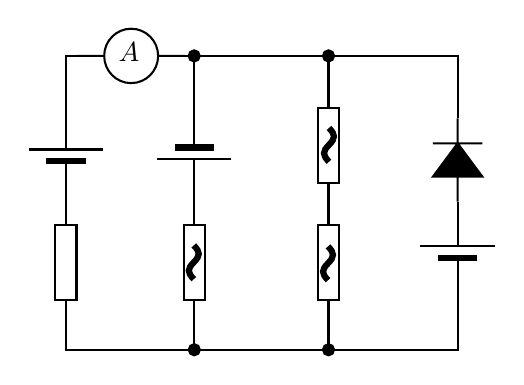
\begin{tikzpicture}[x=0.75pt,y=0.75pt,yscale=-1,xscale=1]
%uncomment if require: \path (0,375); %set diagram left start at 0, and has height of 375

%Shape: Output [id:dp40223434915515366] 
\draw   (144.79,85.1) .. controls (144.79,77.87) and (150.61,72) .. (157.78,72) .. controls (164.96,72) and (170.78,77.87) .. (170.78,85.1) .. controls (170.78,92.34) and (164.96,98.21) .. (157.78,98.21) .. controls (150.61,98.21) and (144.79,92.34) .. (144.79,85.1) -- cycle (131.79,85.1) -- (144.79,85.1) (183.77,85.1) -- (170.78,85.1) ;
%Shape: Right Angle [id:dp45345897491864395] 
\draw   (126.34,108.7) -- (126.34,85.1) -- (131.79,85.1) ;
%Shape: Battery [id:dp26785775847506166] 
\draw  [fill={rgb, 255:red, 0; green, 0; blue, 0 }  ,fill opacity=1 ] (126.34,156.46) -- (126.34,134.97) (108.43,130.19) -- (144.25,130.19) (126.34,130.19) -- (126.34,108.7) (117.39,136.88) -- (117.39,134.97) -- (135.3,134.97) -- (135.3,136.88) -- (117.39,136.88) -- cycle ;
%Shape: Resistor [id:dp428828370029964] 
\draw   (131.46,166.59) -- (131.46,202.59) -- (121.22,202.59) -- (121.22,166.59) -- (131.46,166.59) -- cycle (126.34,156.46) -- (126.34,166.59) (126.34,202.59) -- (126.34,212.72) ;
%Shape: Right Angle [id:dp37458769585276563] 
\draw   (188.21,226.68) -- (126.34,226.68) -- (126.34,212.72) ;
%Straight Lines [id:da02650510741377521] 
\draw    (188.21,212.72) -- (188.21,226.68) ;
\draw [shift={(188.21,226.68)}, rotate = 90] [color={rgb, 255:red, 0; green, 0; blue, 0 }  ][fill={rgb, 255:red, 0; green, 0; blue, 0 }  ][line width=0.75]      (0, 0) circle [x radius= 2.68, y radius= 2.68]   ;
%Shape: Resistor [id:dp5839554899269066] 
\draw   (193.27,166.59) -- (193.27,202.59) -- (183.03,202.59) -- (183.03,166.59) -- (193.27,166.59) -- cycle (188.15,156.46) -- (188.15,166.59) (188.15,202.59) -- (188.15,212.72) ;
%Shape: Battery [id:dp021184207056247795] 
\draw  [fill={rgb, 255:red, 0; green, 0; blue, 0 }  ,fill opacity=1 ] (188.15,108.7) -- (188.15,130.19) (206.06,134.97) -- (170.24,134.97) (188.15,134.97) -- (188.15,156.46) (197.1,128.28) -- (197.1,130.19) -- (179.19,130.19) -- (179.19,128.28) -- (197.1,128.28) -- cycle ;
%Straight Lines [id:da6706541214826243] 
\draw    (188.15,108.7) -- (188.15,85.1) ;
\draw [shift={(188.15,85.1)}, rotate = 270] [color={rgb, 255:red, 0; green, 0; blue, 0 }  ][fill={rgb, 255:red, 0; green, 0; blue, 0 }  ][line width=0.75]      (0, 0) circle [x radius= 2.68, y radius= 2.68]   ;
%Straight Lines [id:da4086835439710659] 
\draw    (183.77,85.1) -- (188.59,85.1) ;
%Straight Lines [id:da2917885452261588] 
\draw    (252.87,212.72) -- (252.87,226.68) ;
\draw [shift={(252.87,226.68)}, rotate = 90] [color={rgb, 255:red, 0; green, 0; blue, 0 }  ][fill={rgb, 255:red, 0; green, 0; blue, 0 }  ][line width=0.75]      (0, 0) circle [x radius= 2.68, y radius= 2.68]   ;
%Straight Lines [id:da14066596429940992] 
\draw    (188.21,226.68) -- (252.87,226.68) ;
%Shape: Resistor [id:dp4045940492883866] 
\draw   (257.99,166.59) -- (257.99,202.59) -- (247.75,202.59) -- (247.75,166.59) -- (257.99,166.59) -- cycle (252.87,156.46) -- (252.87,166.59) (252.87,202.59) -- (252.87,212.72) ;
%Shape: Resistor [id:dp571652007762723] 
\draw   (257.99,110.33) -- (257.99,146.33) -- (247.75,146.33) -- (247.75,110.33) -- (257.99,110.33) -- cycle (252.87,100.2) -- (252.87,110.33) (252.87,146.33) -- (252.87,156.46) ;
%Straight Lines [id:da38917417942454513] 
\draw    (252.87,100.2) -- (252.87,85.1) ;
\draw [shift={(252.87,85.1)}, rotate = 270] [color={rgb, 255:red, 0; green, 0; blue, 0 }  ][fill={rgb, 255:red, 0; green, 0; blue, 0 }  ][line width=0.75]      (0, 0) circle [x radius= 2.68, y radius= 2.68]   ;
%Straight Lines [id:da03606821117235004] 
\draw    (188.59,85.1) -- (253.35,85.1) ;
%Shape: Right Angle [id:dp9058220555439067] 
\draw   (253.35,85.1) -- (315.09,85.1) -- (315.09,115.19) ;
%Shape: Battery [id:dp6694974686185533] 
\draw  [fill={rgb, 255:red, 0; green, 0; blue, 0 }  ,fill opacity=1 ] (315.09,203.05) -- (315.09,181.56) (297.18,176.79) -- (333,176.79) (315.09,176.79) -- (315.09,155.3) (306.14,183.47) -- (306.14,181.56) -- (324.05,181.56) -- (324.05,183.47) -- (306.14,183.47) -- cycle ;
%Shape: Right Angle [id:dp5305063249969073] 
\draw   (315.09,203.05) -- (315.09,226.68) -- (252.87,226.68) ;
%Shape: Diode [id:dp3686655850262377] 
\draw  [fill={rgb, 255:red, 0; green, 0; blue, 0 }  ,fill opacity=1 ] (303.2,143.26) -- (315.09,127.22) -- (326.98,143.26) -- (303.2,143.26) -- cycle (315.09,155.3) -- (315.09,143.26) (303.2,127.22) -- (326.98,127.22) (315.09,127.22) -- (315.09,115.19) ;
%Shape: Sine Wave Form [id:dp14441278202793773] 
\draw  [line width=2.25]  (187.97,176.4) .. controls (191.14,179.71) and (191.15,181.27) .. (187.97,184.54) .. controls (184.78,187.81) and (184.77,189.34) .. (187.97,192.68) ;
%Shape: Sine Wave Form [id:dp4832496115476983] 
\draw  [line width=2.25]  (252.63,176.87) .. controls (255.8,180.19) and (255.81,181.75) .. (252.63,185.02) .. controls (249.44,188.28) and (249.43,189.81) .. (252.63,193.16) ;
%Shape: Sine Wave Form [id:dp029747975461203113] 
\draw  [line width=2.25]  (253.1,119.82) .. controls (256.27,123.13) and (256.29,124.7) .. (253.1,127.96) .. controls (249.92,131.23) and (249.9,132.76) .. (253.1,136.11) ;
% Text Node
\draw (150.28,77.24) node [anchor=north west][inner sep=0.75pt]    {$A$};
\end{tikzpicture}
    \\ Hình 1.
 \end{center}
 Hình 2 mô tả đường cong $I - V$ của diode. Thang đo của điện áp (trục nằm ngang) không được xác định nhưng người ta biết rằng một dòng điện bằng $I_0$ chạy qua diode tương ứng với điện áp bằng $\dfrac{1}{5}$ điện áp của nguồn điện. 
 \begin{center}
    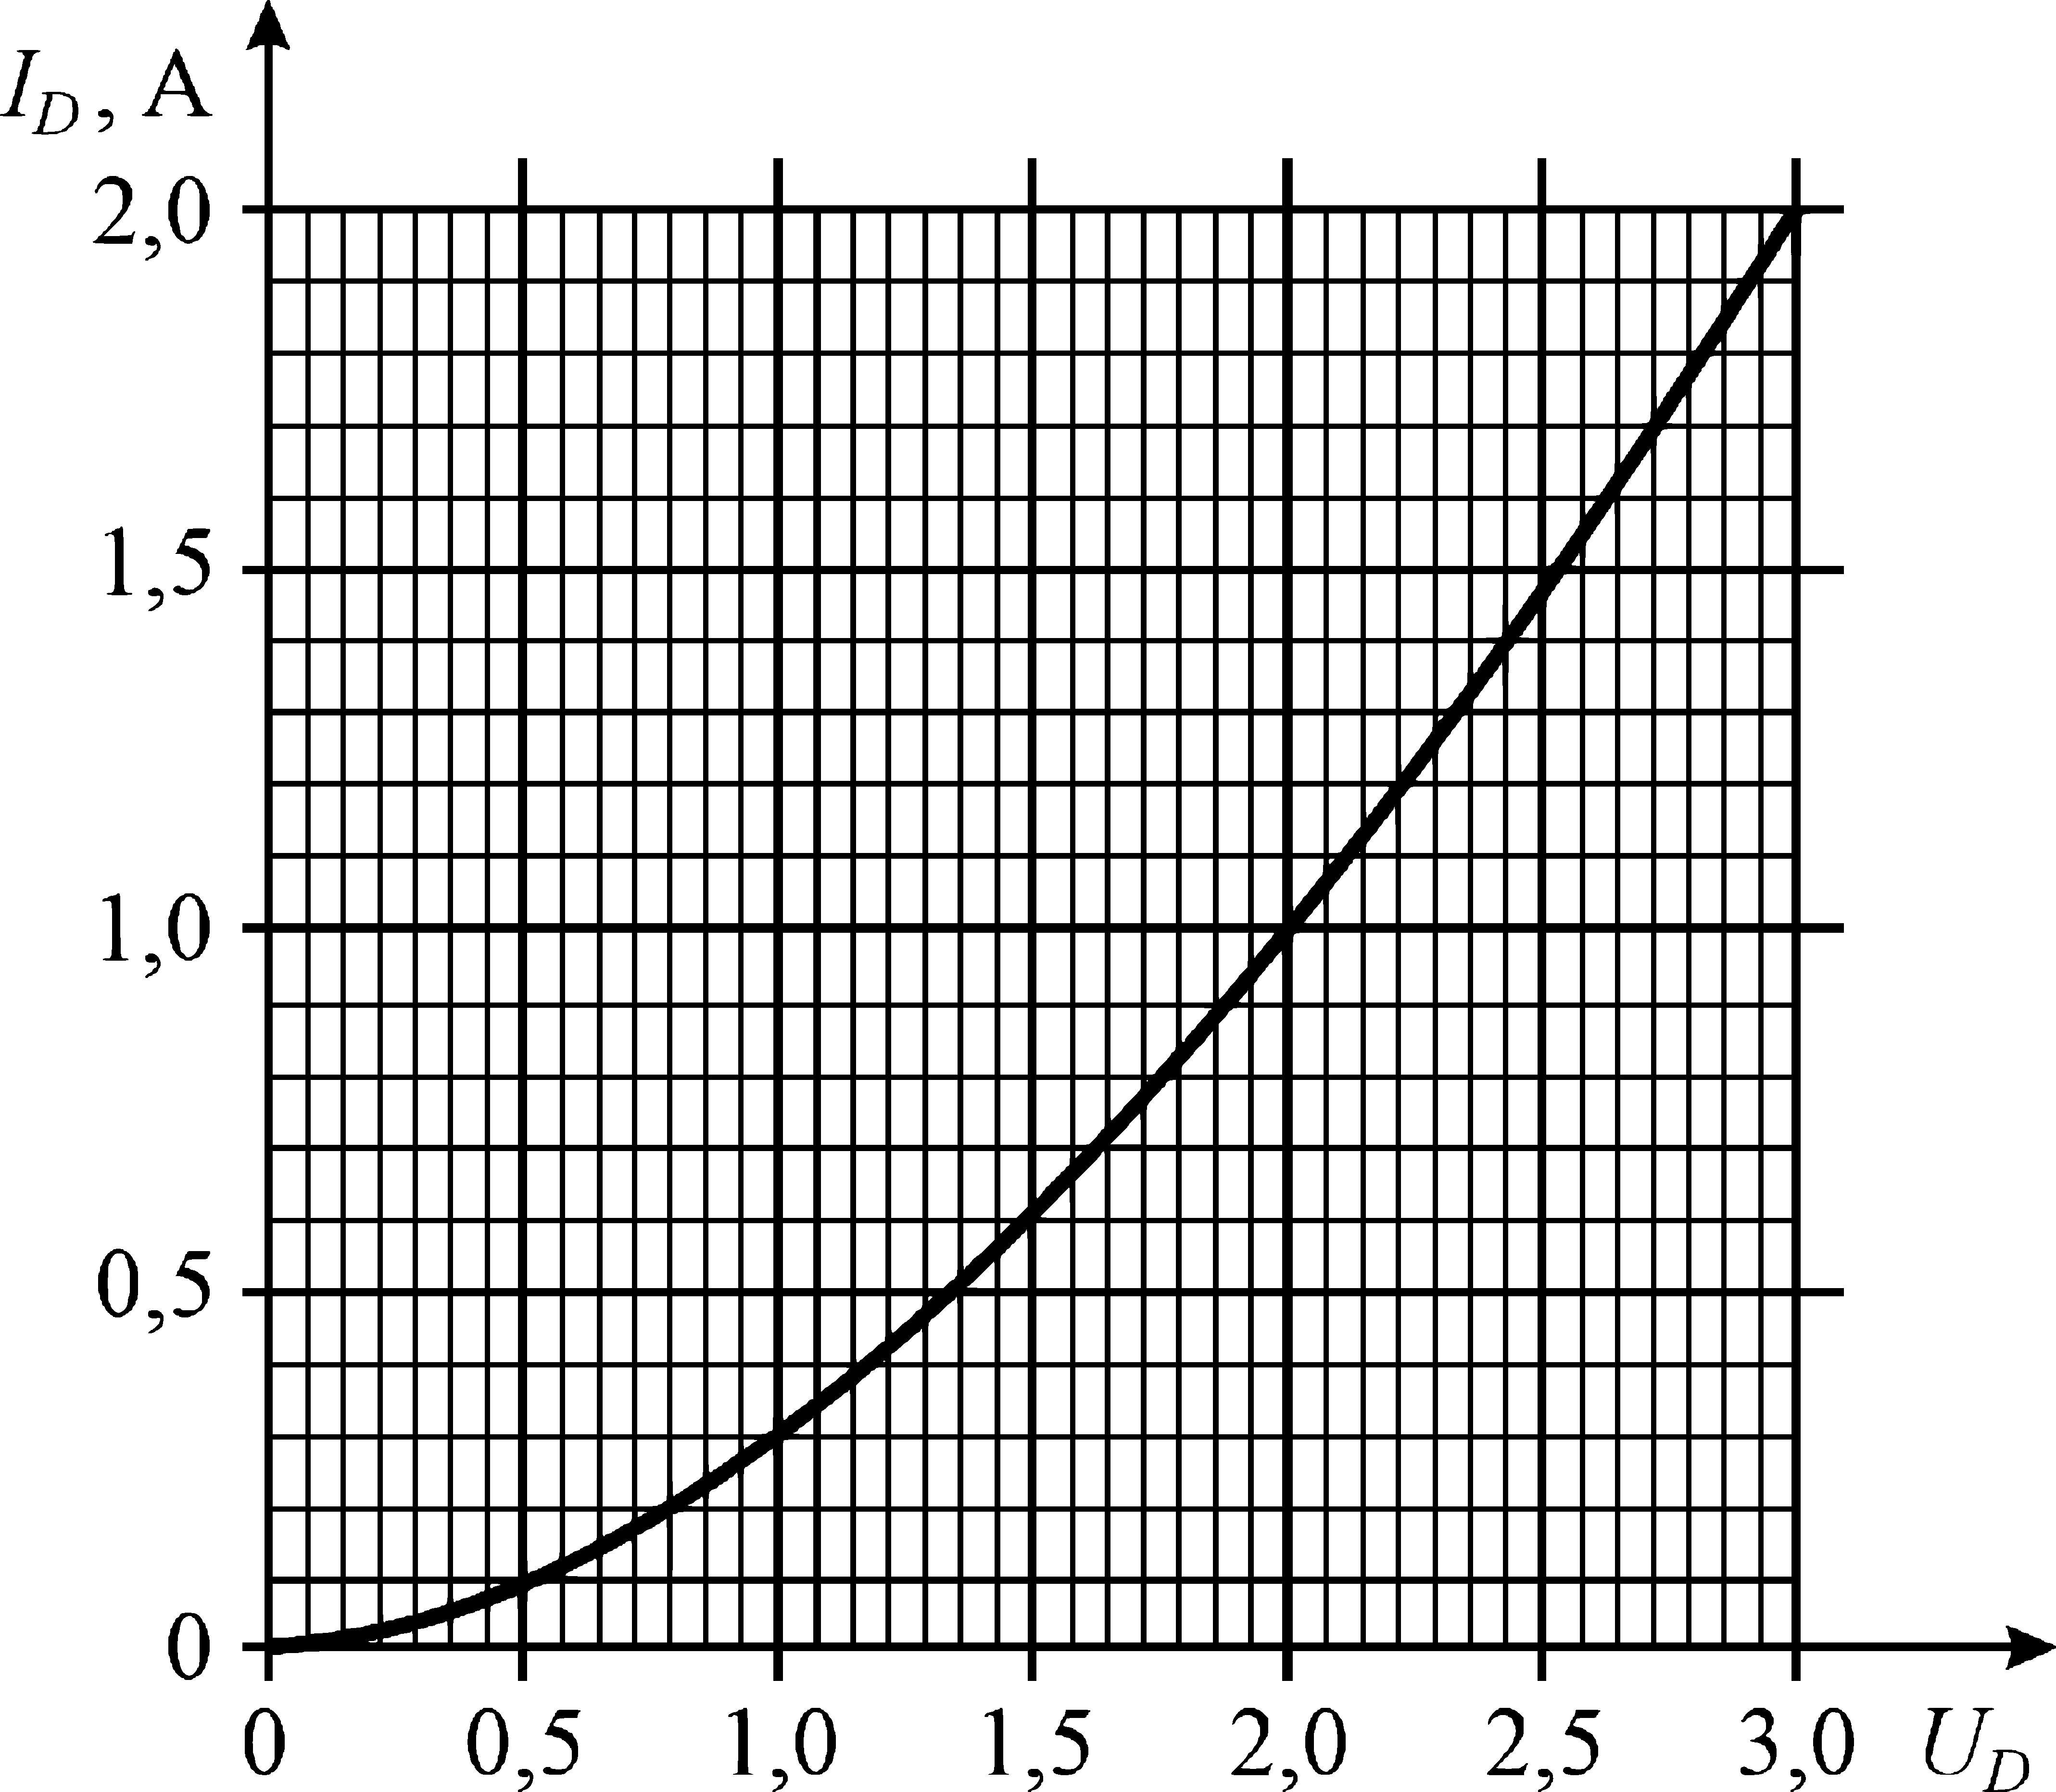
\includegraphics[width=0.7\textwidth]{Anh/iom1.pdf}
     \\Hình 2.
 \end{center}
\begin{enumerate}[1)]
    \item Viết đầy đủ các phương trình cho dòng điện chạy trong các nhánh của mạch điện trong hình 1. Các phương trình phải bao gồm điện áp $U$ của các nhánh song song cùng với điện áp $\xi$ của nguồn điện, điện trở thuần $R$ và hệ số $\alpha$.
    \item Xác định số chỉ của ampe kế với độ  chính xác tối thiểu là $10 \%$. Bỏ qua điện trở của dây dẫn. Viết câu trả lời bằng đơn vị $\mathrm{A}$ và cho biết độ chính xác của kết quả.
\end{enumerate}
\begin{center}
    \bf Phần II: Phi tuyến tính và sự phóng điện của tụ điện.
\end{center}
\immini{Nối varistor có hệ số $\alpha$ với một tụ điện đã được nạp điện (xem hình 3). Nếu dây dẫn được làm lạnh đủ, chúng sẽ trở nên siêu dẫn và tụ điện sẽ xả hết điện trong thời gian $t_0 = 0,02 ~\mathrm{s}$. Biết thuộc tính của varistor không phụ thuộc vào nhiệt độ.}
{


\tikzset{every picture/.style={line width=0.75pt}} %set default line width to 0.75pt        

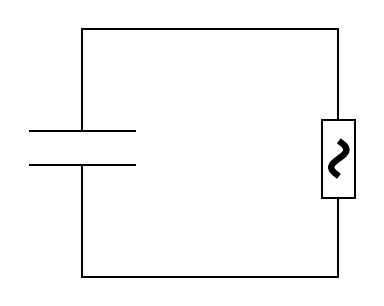
\begin{tikzpicture}[x=0.75pt,y=0.75pt,yscale=-1,xscale=1]
%uncomment if require: \path (0,418); %set diagram left start at 0, and has height of 418

%Shape: Contact [id:dp08886901469143238] 
\draw   (113.85,136.93) -- (113.85,149.1) (113.85,177.5) -- (113.85,165.33) (139.7,149.1) -- (88,149.1) (139.7,165.33) -- (88,165.33) ;
%Shape: Right Angle [id:dp18670073540497323] 
\draw   (113.85,136.93) -- (113.85,99.83) -- (185.67,99.83) ;
%Shape: Right Angle [id:dp6174860778702249] 
\draw   (176.3,219.33) -- (113.85,219.33) -- (113.85,177.5) ;
%Shape: Resistor [id:dp24304015186446315] 
\draw   (245,143.92) -- (245,181.59) -- (229.13,181.59) -- (229.13,143.92) -- (245,143.92) -- cycle (237.07,133.33) -- (237.07,143.92) (237.07,181.59) -- (237.07,192.18) ;
%Shape: Sine Wave Form [id:dp9035485123364762] 
\draw  [line width=2.25]  (237.43,153.86) .. controls (242.34,157.32) and (242.36,158.96) .. (237.43,162.37) .. controls (232.49,165.79) and (232.46,167.39) .. (237.43,170.89) ;
%Shape: Right Angle [id:dp9499664503536653] 
\draw   (185.67,99.83) -- (237.07,99.83) -- (237.07,133.33) ;
%Shape: Right Angle [id:dp5719302324978046] 
\draw   (237.07,192.18) -- (237.07,219.33) -- (176.3,219.33) ;
\end{tikzpicture}
\\Hình 3.
}
\begin{enumerate}[1)]
    \item Biểu diễn $t_0$ theo điện dung $C$, điện tích ban đầu của tụ điện $q_0$ và hệ số $\alpha$ của varistor.
    \item Nếu tụ điện chỉ phóng điện qua các dây nối ở nhiệt độ phòng thì điện tích giảm đi một lượng $e$ trong thời gian $\tau = 1 ~\mathrm{ms}$ ($e$ là cơ số của logarit tự nhiên). Hãy tìm mối liên hệ giữa $\tau$ và điện trở $r$ của dây dẫn, từ đó suy ra phương trình tương ứng.
    \item Xác định thời điểm $t$ mà tại đó đòng điện giảm từ giá trị ban đầu $I_0$ về $I$, giả sử tụ điện chỉ  phóng điện qua varistor ở nhiệt độ phòng. Viết câu trả lời theo $r, C, \alpha, I$ và $I_0$.
    \item Xác định thời điểm $t_1$ mà tại đó điện tích của tụ giảm đi $n = 10 \ 000$ lần, giả sử tụ điện phóng điện qua cả dây dẫn và varistor ở nhiệt độ phòng. Hãy tìm phương trình biểu diễn $t_1$ qua $t_0, \tau$, $n$ và nhận xét giá trị tính bằng số (theo $\mathrm{ms}$) của $t_1$ với độ chính xác tối thiểu $10 \%$. 
\end{enumerate}

\begin{center}
    \bf Phần III: Phi tuyến tính và dao động tắt dần.
\end{center}
\immini{Trong thí nghiệm tiếp theo, mạch điện gồm một tụ điện, một varistor (với hệ số $\alpha$) và cuộn cảm siêu dẫn $L$
(xem hình 4). Các dây dẫn cũng được duy trì ở trạng thái siêu dẫn. Trong trường hợp này, dao động tắt dần bắt đầu trong
mạch và khi dòng điện biến mất lần đầu tiên, điện tích của tụ điện nhỏ hơn giá trị ban đầu $10 \%$.}
{

\tikzset{every picture/.style={line width=0.75pt}} %set default line width to 0.75pt        

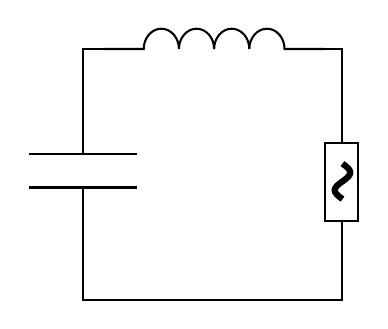
\begin{tikzpicture}[x=0.75pt,y=0.75pt,yscale=-1,xscale=1]
%uncomment if require: \path (0,418); %set diagram left start at 0, and has height of 418

%Shape: Contact [id:dp26517604501135117] 
\draw   (251.32,138.89) -- (251.32,151.11) (251.32,179.64) -- (251.32,167.42) (277.47,151.11) -- (225.17,151.11) (277.47,167.42) -- (225.17,167.42) ;
%Shape: Right Angle [id:dp8160408833509483] 
\draw   (251.32,138.89) -- (251.32,100.67) -- (261.5,100.67) ;
%Shape: Right Angle [id:dp7364908678000435] 
\draw   (314.5,221.67) -- (251.32,221.67) -- (251.32,179.64) ;
%Shape: Resistor [id:dp26655342074498534] 
\draw   (384,145.91) -- (384,183.75) -- (367.94,183.75) -- (367.94,145.91) -- (384,145.91) -- cycle (375.97,135.27) -- (375.97,145.91) (375.97,183.75) -- (375.97,194.39) ;
%Shape: Sine Wave Form [id:dp947924618662443] 
\draw  [line width=2.25]  (376.34,155.89) .. controls (381.3,159.37) and (381.33,161.01) .. (376.34,164.45) .. controls (371.34,167.88) and (371.31,169.49) .. (376.34,173) ;
%Shape: Right Angle [id:dp3971851855646844] 
\draw   (348.42,100.67) -- (375.97,100.67) -- (375.97,135.27) ;
%Shape: Right Angle [id:dp2129631794566038] 
\draw   (375.97,194.39) -- (375.97,221.67) -- (314.5,221.67) ;
%Shape: Inductor (Air Core) [id:dp547707303950224] 
\draw   (261.5,100.67) -- (280.58,100.67) .. controls (280.58,95.28) and (284.38,90.9) .. (289.06,90.9) .. controls (293.74,90.9) and (297.54,95.28) .. (297.54,100.67) .. controls (297.54,95.28) and (301.34,90.9) .. (306.02,90.9) .. controls (310.7,90.9) and (314.5,95.28) .. (314.5,100.67) .. controls (314.5,95.28) and (318.3,90.9) .. (322.98,90.9) .. controls (327.66,90.9) and (331.46,95.28) .. (331.46,100.67) .. controls (331.46,95.28) and (335.26,90.9) .. (339.94,90.9) .. controls (344.62,90.9) and (348.42,95.28) .. (348.42,100.67) -- (367.5,100.67) ;
\end{tikzpicture}
\\Hình 4.}
\begin{enumerate}[1)]
    \item Giả sử rằng tại một thời điểm nào đó trước khi kết thúc nửa chu kỳ dao động đầu tiên, điện tích của tụ điện đã giảm từ giá trị ban đầu $q_0$ xuống $q$. Dòng điện trong mạch lúc này bằng bao nhiêu? Biễu diễn kết quả theo $\alpha, L, C, q$ và $q_0$. Sẽ rất hữu ích khi biết rằng lời giải của một phương trình phi tuyến phức tạp của chuyển động cơ học thường được đơn giản hóa đáng kể nếu biến nó thành một phương trình cho tốc độ biến thiên năng lượng.
    \item Xác định năng lượng của tụ điện được giải phóng dưới dạng nhiệt trong varistor cho đến khi điện tích tụ của điện bằng không lần đầu tiên. Đánh giá câu trả lời (theo phần trăm) với độ chính xác tối thiểu $10 \%$ (nghĩa là sai số không được vượt quá $10\%$ kết quả).
    \item Phần nào của năng lượng ban đầu của tụ điện được giải phóng dưới dạng nhiệt trong varistor cho đến khi dòng điện bằng không lần đầu tiên? Đánh giá câu trả lời theo phần trăm.
    \item Phần nào của năng lượng ban đầu của tụ điện được giải phóng dưới dạng nhiệt trong varistor tại thời điểm điện tích của tụ điện bằng không lần thứ hai? Đánh giá câu trả lời (theo phần trăm) với độ chính xác tối thiểu $10 \%$ (nghĩa là sai số không được vượt quá $10\%$ kết quả).
\end{enumerate}
\textbf{Lưu ý.} Hệ số $\alpha$ của varistor trong mỗi phần của bài toán là khác nhau!
\end{vd}
\begin{loigiai}\[\]
\textbf{Phần I.}
\begin{enumerate}[1)]
    \item Các kí hiệu sẽ sử dụng trong bài toán: gọi $U$ là hiệu điện thế chung của bốn nhánh song song (giữa dây dẫn ngang phía trên và phía dưới), $I_{1,2,3,4}$ là dòng điện chạy qua các nhánh (theo thứ tự từ trái sang phải, chiều dương của các dòng điện được thể hiện bằng các mũi tên như trong hình 1a).
    \begin{center}
        

\tikzset{every picture/.style={line width=0.75pt}} %set default line width to 0.75pt        

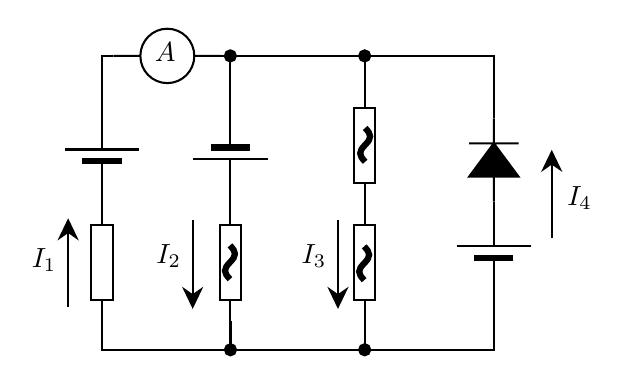
\begin{tikzpicture}[x=0.75pt,y=0.75pt,yscale=-1,xscale=1]
%uncomment if require: \path (0,375); %set diagram left start at 0, and has height of 375

%Shape: Output [id:dp40223434915515366] 
\draw   (144.79,85.1) .. controls (144.79,77.87) and (150.61,72) .. (157.78,72) .. controls (164.96,72) and (170.78,77.87) .. (170.78,85.1) .. controls (170.78,92.34) and (164.96,98.21) .. (157.78,98.21) .. controls (150.61,98.21) and (144.79,92.34) .. (144.79,85.1) -- cycle (131.79,85.1) -- (144.79,85.1) (183.77,85.1) -- (170.78,85.1) ;
%Shape: Right Angle [id:dp45345897491864395] 
\draw   (126.34,108.7) -- (126.34,85.1) -- (131.79,85.1) ;
%Shape: Battery [id:dp26785775847506166] 
\draw  [fill={rgb, 255:red, 0; green, 0; blue, 0 }  ,fill opacity=1 ] (126.34,156.46) -- (126.34,134.97) (108.43,130.19) -- (144.25,130.19) (126.34,130.19) -- (126.34,108.7) (117.39,136.88) -- (117.39,134.97) -- (135.3,134.97) -- (135.3,136.88) -- (117.39,136.88) -- cycle ;
%Shape: Resistor [id:dp428828370029964] 
\draw   (131.46,166.59) -- (131.46,202.59) -- (121.22,202.59) -- (121.22,166.59) -- (131.46,166.59) -- cycle (126.34,156.46) -- (126.34,166.59) (126.34,202.59) -- (126.34,212.72) ;
%Shape: Right Angle [id:dp37458769585276563] 
\draw   (188.21,226.68) -- (126.34,226.68) -- (126.34,212.72) ;
%Straight Lines [id:da02650510741377521] 
\draw    (188.21,212.72) -- (188.21,226.68) ;
\draw [shift={(188.21,226.68)}, rotate = 90] [color={rgb, 255:red, 0; green, 0; blue, 0 }  ][fill={rgb, 255:red, 0; green, 0; blue, 0 }  ][line width=0.75]      (0, 0) circle [x radius= 2.68, y radius= 2.68]   ;
%Shape: Resistor [id:dp5839554899269066] 
\draw   (193.27,166.59) -- (193.27,202.59) -- (183.03,202.59) -- (183.03,166.59) -- (193.27,166.59) -- cycle (188.15,156.46) -- (188.15,166.59) (188.15,202.59) -- (188.15,212.72) ;
%Shape: Battery [id:dp021184207056247795] 
\draw  [fill={rgb, 255:red, 0; green, 0; blue, 0 }  ,fill opacity=1 ] (188.15,108.7) -- (188.15,130.19) (206.06,134.97) -- (170.24,134.97) (188.15,134.97) -- (188.15,156.46) (197.1,128.28) -- (197.1,130.19) -- (179.19,130.19) -- (179.19,128.28) -- (197.1,128.28) -- cycle ;
%Straight Lines [id:da6706541214826243] 
\draw    (188.15,108.7) -- (188.15,85.1) ;
\draw [shift={(188.15,85.1)}, rotate = 270] [color={rgb, 255:red, 0; green, 0; blue, 0 }  ][fill={rgb, 255:red, 0; green, 0; blue, 0 }  ][line width=0.75]      (0, 0) circle [x radius= 2.68, y radius= 2.68]   ;
%Straight Lines [id:da4086835439710659] 
\draw    (183.77,85.1) -- (188.59,85.1) ;
%Straight Lines [id:da2917885452261588] 
\draw    (252.87,212.72) -- (252.87,226.68) ;
\draw [shift={(252.87,226.68)}, rotate = 90] [color={rgb, 255:red, 0; green, 0; blue, 0 }  ][fill={rgb, 255:red, 0; green, 0; blue, 0 }  ][line width=0.75]      (0, 0) circle [x radius= 2.68, y radius= 2.68]   ;
%Straight Lines [id:da14066596429940992] 
\draw    (188.21,226.68) -- (252.87,226.68) ;
%Shape: Resistor [id:dp4045940492883866] 
\draw   (257.99,166.59) -- (257.99,202.59) -- (247.75,202.59) -- (247.75,166.59) -- (257.99,166.59) -- cycle (252.87,156.46) -- (252.87,166.59) (252.87,202.59) -- (252.87,212.72) ;
%Shape: Resistor [id:dp571652007762723] 
\draw   (257.99,110.33) -- (257.99,146.33) -- (247.75,146.33) -- (247.75,110.33) -- (257.99,110.33) -- cycle (252.87,100.2) -- (252.87,110.33) (252.87,146.33) -- (252.87,156.46) ;
%Straight Lines [id:da38917417942454513] 
\draw    (252.87,100.2) -- (252.87,85.1) ;
\draw [shift={(252.87,85.1)}, rotate = 270] [color={rgb, 255:red, 0; green, 0; blue, 0 }  ][fill={rgb, 255:red, 0; green, 0; blue, 0 }  ][line width=0.75]      (0, 0) circle [x radius= 2.68, y radius= 2.68]   ;
%Straight Lines [id:da03606821117235004] 
\draw    (188.59,85.1) -- (253.35,85.1) ;
%Shape: Right Angle [id:dp9058220555439067] 
\draw   (253.35,85.1) -- (315.09,85.1) -- (315.09,115.19) ;
%Shape: Battery [id:dp6694974686185533] 
\draw  [fill={rgb, 255:red, 0; green, 0; blue, 0 }  ,fill opacity=1 ] (315.09,203.05) -- (315.09,181.56) (297.18,176.79) -- (333,176.79) (315.09,176.79) -- (315.09,155.3) (306.14,183.47) -- (306.14,181.56) -- (324.05,181.56) -- (324.05,183.47) -- (306.14,183.47) -- cycle ;
%Shape: Right Angle [id:dp5305063249969073] 
\draw   (315.09,203.05) -- (315.09,226.68) -- (252.87,226.68) ;
%Shape: Diode [id:dp3686655850262377] 
\draw  [fill={rgb, 255:red, 0; green, 0; blue, 0 }  ,fill opacity=1 ] (303.2,143.26) -- (315.09,127.22) -- (326.98,143.26) -- (303.2,143.26) -- cycle (315.09,155.3) -- (315.09,143.26) (303.2,127.22) -- (326.98,127.22) (315.09,127.22) -- (315.09,115.19) ;
%Shape: Sine Wave Form [id:dp14441278202793773] 
\draw  [line width=2.25]  (187.97,176.4) .. controls (191.14,179.71) and (191.15,181.27) .. (187.97,184.54) .. controls (184.78,187.81) and (184.77,189.34) .. (187.97,192.68) ;
%Shape: Sine Wave Form [id:dp4832496115476983] 
\draw  [line width=2.25]  (252.63,176.87) .. controls (255.8,180.19) and (255.81,181.75) .. (252.63,185.02) .. controls (249.44,188.28) and (249.43,189.81) .. (252.63,193.16) ;
%Shape: Sine Wave Form [id:dp029747975461203113] 
\draw  [line width=2.25]  (253.1,119.82) .. controls (256.27,123.13) and (256.29,124.7) .. (253.1,127.96) .. controls (249.92,131.23) and (249.9,132.76) .. (253.1,136.11) ;
%Straight Lines [id:da45555386757583727] 
\draw    (110,206) -- (110,166.33) ;
\draw [shift={(110,163.33)}, rotate = 450] [fill={rgb, 255:red, 0; green, 0; blue, 0 }  ][line width=0.08]  [draw opacity=0] (10.72,-5.15) -- (0,0) -- (10.72,5.15) -- (7.12,0) -- cycle    ;
%Straight Lines [id:da5648832182011037] 
\draw    (343,173) -- (343,133.33) ;
\draw [shift={(343,130.33)}, rotate = 450] [fill={rgb, 255:red, 0; green, 0; blue, 0 }  ][line width=0.08]  [draw opacity=0] (10.72,-5.15) -- (0,0) -- (10.72,5.15) -- (7.12,0) -- cycle    ;
%Straight Lines [id:da8180273933014601] 
\draw    (170,204) -- (170,164.33) ;
\draw [shift={(170,207)}, rotate = 270] [fill={rgb, 255:red, 0; green, 0; blue, 0 }  ][line width=0.08]  [draw opacity=0] (10.72,-5.15) -- (0,0) -- (10.72,5.15) -- (7.12,0) -- cycle    ;
%Straight Lines [id:da8943686905317443] 
\draw    (240,204) -- (240,164.33) ;
\draw [shift={(240,207)}, rotate = 270] [fill={rgb, 255:red, 0; green, 0; blue, 0 }  ][line width=0.08]  [draw opacity=0] (10.72,-5.15) -- (0,0) -- (10.72,5.15) -- (7.12,0) -- cycle    ;

% Text Node
\draw (150.28,77.24) node [anchor=north west][inner sep=0.75pt]    {$A$};
% Text Node
\draw (91,176.4) node [anchor=north west][inner sep=0.75pt]    {$I_{1}$};
% Text Node
\draw (349,146.4) node [anchor=north west][inner sep=0.75pt]    {$I_{4}$};
% Text Node
\draw (151,174.4) node [anchor=north west][inner sep=0.75pt]    {$I_{2}$};
% Text Node
\draw (221,174.4) node [anchor=north west][inner sep=0.75pt]    {$I_{3}$};
\end{tikzpicture}
        \\Hình 1a.
    \end{center}
    $R$ là giá trị của điện trở thuần. Từ đề bài, ta thấy $R = \dfrac{\xi}{I_0}$.\\
    Vì dòng điện và điện áp của varistor liên hệ với nhau bởi phương trình $U = \alpha I\abs{I}$, nên từ điều kiện đề bài, ta suy ra $\alpha = \dfrac{\xi}{I_0^2}$. Giả sử rằng đặc tính $I - V$ của diode là $I_D = I_0 \cdot f\tron{U_D/\xi}$. Khi đó, dòng điện qua các nhánh có thể được biểu diễn thông qua điện áp trên chúng như sau:
    \[\heva{I_1 &= \dfrac{\xi - U}{R} = I_0 (1-x) \\ 
    \alpha I_2^2 &= U+\xi \rt I_2 = I_0 \sqrt{1+x} \\ 
    2\alpha I_3^2 &= U \rt I_3 = I_0 \sqrt{\dfrac{x}{2}} \\ 
    I_4 &= I_0 f(1-x) },\]
    trong đó $x = \dfrac{U}{\xi}$ (sự chính xác của chiều dương các dòng điện đã chọn được xác minh trong quá trình giải). Ngoài ra, dòng điện phải thoả mãn định luật bảo toàn điện tích $I_2 + I_3 = I_1 + I_4$. Do đó, $x$ có thể xác định được qua phương trình: \[\sqrt{1+x} + \sqrt{\dfrac{x}{2}} = 1-x +  f(1-x).\]
    \item Theo đề bài, dòng điện qua diode bằng $I_0$ khi điện áp của diode bằng $\dfrac{1}{5}\xi$. Do đó, $f(0,2) = 1$, cho phép ta ``dịch chuyển'' đường cong $I-V$ của diode trên đồ thị, các dòng điện qua các nhánh khác được vẽ trên hình (đường cong màu đỏ trong hình 1b) và để giải phương trình trên bằng đồ thị: vẽ biểu đồ bên trái của phương trình và sau đó vẽ biểu đồ bên phải bằng cách cộng các đóng góp của các dòng điện tại mỗi $x$. \\
    Theo đồ thị, số chỉ của ampe kế (ứng với cường độ dòng điện qua điện trở) là $I_A = (0,27 \pm 0,02)~\mathrm{A}$. Sai số này đáp ứng được yêu cầu về độ chính xác cần thiết trong đề bài, ngay cả khi dưới độ chính xác này, nó có thể được cải thiện.
    \begin{center}
    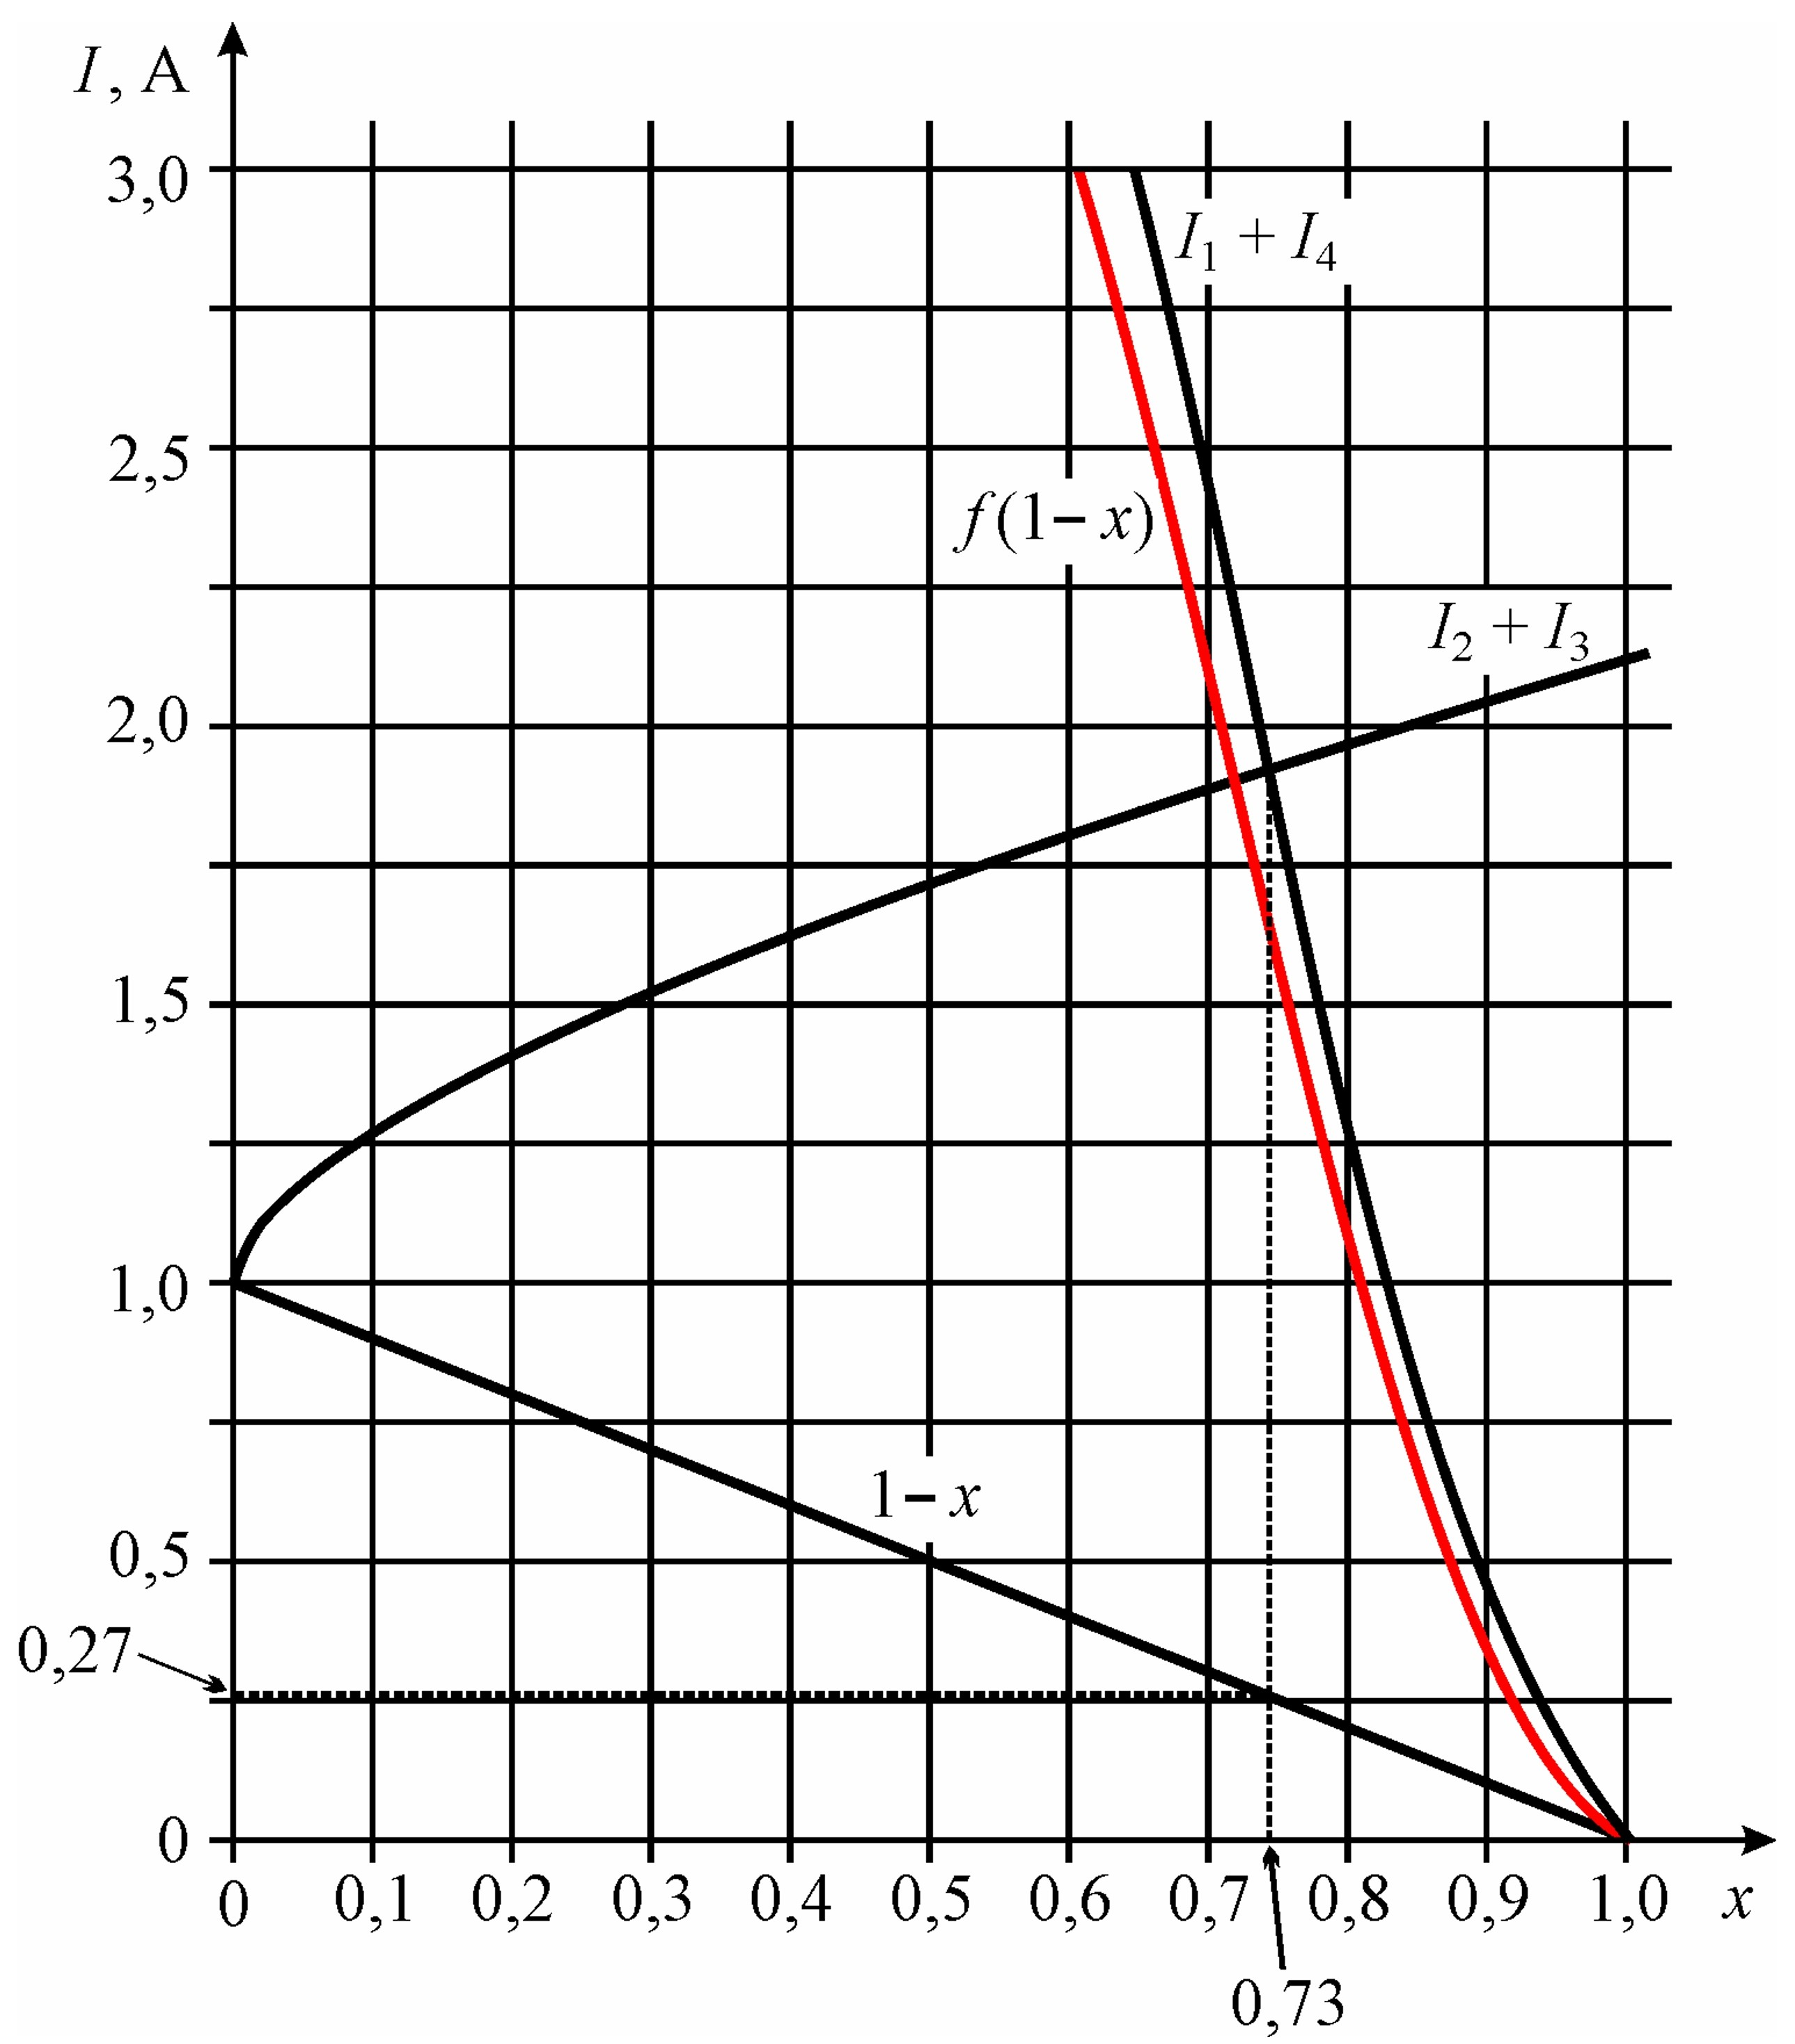
\includegraphics[scale=0.7]{Anh/IOM2018_2.jpg}
       \\ Hình 1b.
    \end{center}
\textbf{Lưu ý.} Kết quả thu được bằng phương pháp đồ thị có thể được cải thiện đáng kể khi sử dụng đại số. Ngay cả cách xây dựng thô sơ của đồ thị cũng giúp xác định rõ đáp án là  $x \approx 0,7$, và  $\left. f((1-x)\right|_{x \approx 0,7} \approx 9 - 10x$. Giả sử $x = 0,7 + \delta$ và sử dụng khai triển bậc nhất theo $\delta$, ta được 
\[\sqrt{1,7} + \sqrt{0,35} + \dfrac{1}{2} \tron{\dfrac{1}{\sqrt{1,7}} + \dfrac{1}{\sqrt{1,4}}} \delta = 2,3 - 11\delta.\]
Vậy $\delta \approx 0,0343$, vì vậy việc sửa chữa thực sự là nhỏ và sai số do tính toán ở đây là dưới $3 \%$. Sai số của đồ thị có thể được ước tính là $2\%$, do đó 
\[I_A = I_0 (1-x) \approx (0,266 \pm 0,011)~\mathrm{A}.\]
Người ta có thể thực hiện bước tiếp theo và đánh giá tiếp tuyến của đường cong diode $I-V$ tại dòng điện bằng $1,6~ \mathrm{A}$ (đây là dòng điện qua diode thu được bằng phép gần đúng thô sơ) và đánh giá các đạo hàm thứ hai, đường cong $I-V$ có thể được mô tả bằng một phương trình bậc hai. Khi làm như vậy, một lỗi tính toán trở nên không đáng kể so với lỗi đồ thị và độ chính xác còn cải thiện nhiều hơn: 
\[I_A \approx (0.267 \pm 0.005)~\mathrm{A}.\]
Tuy nhiên, độ chính xác của phương pháp đồ họa đủ để giải quyết vấn đề với điều kiện việc xây dựng là chính xác. Tuy nhiên, trong tiêu chí đánh giá có một phần thưởng bổ sung được dành riêng cho những người dự thi giảm lỗi gấp đôi so với lỗi được chỉ định trong đề bài. Lưu ý rằng một câu trả lời ''gần như chính xác'' thu được bằng một phương trình giải tích cho đường cong I-V của diode (phương trình này đã được các tác giả biết đến) là:
\[I_A \approx (0,26723 \pm 0,00001) ~\mathrm{A}.\]
\end{enumerate}
\begin{center}
    \bf Phần II.
\end{center}
\begin{enumerate}[1)]
    \item Một lần nữa, ta sử dụng đặc tính phi tuyến dòng điện-điện áp của varistor: $U = \alpha I\abs{I}$. Dòng điện chạy qua varistor thông qua dây siêu dẫn liên hệ với điện tích của tụ điện như sau:
    \[\dfrac{q}{C} = \alpha I^2 \rt I=\sqrt{\dfrac{q}{\alpha C}},\]
    (dòng điện này không đổi chiều và có thể xem là luôn dương). Một biểu thức cho tốc độ biến thiên điện tích:
    \[\dfrac{\dd q}{\dd t} = -I = -\sqrt{\dfrac{q}{\alpha C}},\]
    (điện tích của tụ điện đang giảm), do đó, thời gian xả hết điện: 
    \[t_{0} = \sqrt{\alpha C} \int_{0}^{q_{0}} \dfrac{\dd q}{\sqrt{q}}=2 \sqrt{\alpha C q_{0}},\]
    (trong đó $q_0$ là điện tích ban đầu của tụ). 
    \item Từ đề bài, ta dễ dàng nhận ra rằng:
    \[\dfrac{q}{C} = rI = r\dfrac{\dd q}{\dd t} \rt \tau = Cr \ln{e} = rC\]
    Vậy $\tau$ là một hằng số thời gian cho sự phóng điện của tụ qua dây dẫn ở nhiệt độ phòng, nghĩa là $\tau = rC$.
    \item Hãy viết một phương trình cho sự phóng điện qua varistor và dây dẫn có điện trở $r$. Trong trường hợp này:
    \[\dfrac{q}{C} = \alpha I^{2}+r I \Rightarrow q = C\left(\alpha I^{2}+r I\right),\]
    do đó:
    \[\dfrac{\dd q}{\dd t} = -I = C(2 \alpha I+r) \dfrac{\dd I}{\dd t}.\]
    Vậy thời gian để  dòng điện giảm từ $I_0$ về $I$ là:
    \[t = C \int_{I}^{I_{0}} \dd I\left(\dfrac{r}{I}+2 \alpha\right)=r C \ln \left(\dfrac{I_{0}}{I}\right)+2 \alpha C\left(I_{0}-I\right).\]
    \item Cường độ dòng điện ban đầu trong mạch được xác định bởi:
    \[\dfrac{q_{0}}{C} = \alpha I_{0}^{2}+r I_{0} \Rightarrow I_{0} = \dfrac{r}{2 \alpha}\left[\sqrt{\dfrac{4 \alpha q_{0}}{C r^{2}}+1}-1\right].\]
    Dòng điện trong mạch tại thời điểm điện tích tụ giảm đi $n$ lần là
    \[I=\dfrac{r}{2 \alpha}\left[\sqrt{\dfrac{4 \alpha q_{0}}{n C r^{2}}+1}-1\right].\]
    Dễ dàng nhận thấy rằng:
    \[\dfrac{4 \alpha q_{0}}{C r^{2}}=\dfrac{4 \alpha C q_{0}}{(C r)^{2}}=\dfrac{t_{0}^{2}}{\tau^{2}},\]
    do đó thời gian cần tìm là:
    \[t=\tau \ln \left(\dfrac{\sqrt{\left(t_{0} / \tau\right)^{2}+1}-1}{\sqrt{\left(t_{0} / \tau \sqrt{n}\right)^{2}+1}-1}\right)+\sqrt{t_{0}^{2}+\tau^{2}}-\sqrt{\dfrac{t_{0}^{2}}{n}+\tau^{2}}.\]
    Ta có thể đánh giá giá trị số trực tiếp bằng công thức này (cho kết quả $t \approx 25,873 \mathrm{ms}$), hoặc  có thể thử đơn giản hóa công thức trước. Để làm điều này, hãy lưu ý rằng: $\dfrac{t_{0}^{2}}{\tau^{2}} \gg 1$ và $\dfrac{t_{0}^{2}}{n \tau^{2}} \ll 1$. Suy ra:
    \[t \approx t_{0} + \tau \ln \left(\dfrac{2 n \tau}{e t_{0}}\right) \approx 25,9 \mathrm{~ms}.\]
    Câu trả lời này đáp ứng các yêu cầu về độ chính xác.
    \textbf{Nhận xét.} Kết quả rất thú vị vì một điện trở nhỏ (về mặt số học, $\tau$  chỉ bằng $5\%$ của $t_0$) lại có thể thay đổi kết quả đến gần như $30\%$! Trên thực tế, điện trở của dây thay đổi đáng kể giá trị của $q(t)$ quanh $q=0$: nó kéo dài thời gian phóng điện.
\end{enumerate}
\begin{center}
    \bf Phần III.
\end{center}
\begin{enumerate}[1)]
    \item Hãy viết phương trình dao động trong mạch. Giống như trước, ta giả sử dòng điện của tụ điện là
    \[I = -\dfrac{\dd q}{\dd t}>0,\]
    (tức bây giờ, ta giới hạn một lời giải cho nửa chu kỳ đầu tiên):
    \[\dfrac{q}{C}=\alpha I^{2}+L \dfrac{\dd I}{\dd t} \Rightarrow \dfrac{\dd I}{\dd t}+\dfrac{\alpha}{L} I^{2}=\dfrac{q}{L C}.\]
    Để phân tích tốc độ biến thiên điện tích tụ điện và năng lượng cuộn cảm, ta chỉ cần liên hệ giữa điện tích và cường độ dòng điện, nếu sự phụ thuộc vào thời gian của các đại lượng này là không cần thiết. Bây giờ, chúng ta đánh giá tốc độ biến thiên của động năng trong cơ học:
    \[m \dfrac{\dd V}{\dd t} = F(x, V) \Rightarrow m \dfrac{V \dd V}{V \dd t} = F(x, V) \Rightarrow \dfrac{\dd}{\dd x}\left(\dfrac{V^{2}}{2}\right)=\dfrac{F(x, V)}{m}.\]
    Bằng cách tương tự, công thức trên cho đạo hàm theo thời gian của dòng điện có thể được biến đổi thành
    \[\dfrac{\dd I}{\dd t}=I \dfrac{\dd I}{I \dd t}=-I \dfrac{\dd I}{\dd q}=-\dfrac{1}{2} \dfrac{\dd\left(I^{2}\right)}{\dd q}.\]
    Ta thu được một phương trình cho $I^{2}(q)$:
    \[\dfrac{\dd\left(I^{2}\right)}{\dd q}-\dfrac{2 \alpha}{L} I^{2}=-\dfrac{2 q}{L C}.\]
    Phương trình tương tự sau đây nếu người ta áp dụng một đối số tương tự cho tốc độ biến thiên của năng lượng tích trữ trong mạch.\\
    Có thể loại bỏ vế phải bằng cách thay thế tuyến tính $\tilde{I}^{2}(q)=A q+B$, phương trình trở thành
    \[\heva{-\dfrac{2 \alpha}{L} A = -\dfrac{2}{L C} \\
    A-\dfrac{2 \alpha}{L} B = 0} \rt \tilde{I}^{2}(q)=\dfrac{q}{\alpha C}+\dfrac{L}{2 \alpha^{2} C}.\]
    Sau đó, ta có thể thay đổi các biến bằng cách viết:
    \[I^{2}(q)=\tilde{I}^{2}(q)+F(q)=\dfrac{q}{\alpha C}+\dfrac{L}{2 \alpha^{2} C}+F(q),\]
    phương trình trở thành:
    \[\dfrac{\dd F}{\dd q}-\dfrac{2 \alpha}{L} F=0.\]
    Như vậy
    \[F(q)=D \cdot \exp \left(\frac{2 \alpha}{L} q\right),\]
    (trong đó $D = \const$), nên $I^{2}(q)$  trong nửa chu kỳ dao động đầu bằng:
    \[I^{2}(q) = \dfrac{q}{\alpha C}+\dfrac{L}{2 \alpha^{2} C}+D \cdot \exp \left(\dfrac{2 \alpha}{L} q\right).\]
    Nếu $q_0$ là điện tích ban đầu của tụ thì $I^{2}\left(q_{0}\right)=0$. Do đó
    \[D = -\dfrac{1}{\alpha C}\left(\dfrac{L}{2 \alpha}+q_{0}\right) \cdot \exp \left(-\dfrac{2 \alpha}{L} q_{0}\right),\]
    kết quả cuối cùng là
    \[I(q)=\sqrt{\dfrac{1}{\alpha C}\left\{\dfrac{L}{2 \alpha}+q-\left(\dfrac{L}{2 \alpha}+q_{0}\right) \cdot \exp \left(\dfrac{2 \alpha}{L}\left(q-q_{0}\right)\right)\right\}}.\]
    \item Dòng điện biến mất lần đầu tại thời điểm kết thúc nửa chu kỳ dao động đầu tiên, khi điện tích của tụ đổi cực và bằng $q_1 = - 0.9 q_0$. Do đó, $I^{2}\left(-0,9 q_{0}\right)=0$ và phương trình này giúp ta xác định điện tích ban đầu của tụ điện. Để cho thuận tiện, ta đặt một biến mới $z \equiv \dfrac{2 \alpha}{L} q_{0}$, khi đó 
    \[1 - 0.9 z - (1+z) e^{-1.9 z}=0 \Rightarrow e^{1.9 z} = \dfrac{1+z}{1-0.9 z}.\]
    Phương trình cũng có thể được giải một cách thủ công. Để làm điều này, trước tiên ta có thể nhận thấy từ đồ thị là $z \ll 1$ và sau đó khai triển hai vế đến bậc thứ tư (điều này là cần thiết ví các bậc không và một bị triệt tiêu):
    \[\dfrac{(1.9)^{2}}{2} z^{2}+\dfrac{(1.9)^{3}}{6} z^{3}+\dfrac{(1.9)^{4}}{24} z^{4} \approx 1.9 \cdot 0.9 z^{2}+1.9 \cdot(0.9)^{2} z^{3}+1.9 \cdot(0.9)^{3} z^{4}.\]
    Điều này cho một phương trình bậc hai  theo $z$, nghiệm dương của nó là $z \approx 0.17$. Sai số của bặc $z^2$ là nhỏ hơn $3 \%$, do đó đáp ứng được yêu cầu bài toán  (khai triển lên đến bậc $z^3$ tạo ra một phương trình tuyến tính nhưng sai số là của bậc $z$ và điều này là không đủ chính xác; kết quả tính được là $x \approx 0.24$ sai lệch so với câu trả lời đúng hơn $10\%$). Một đáp án tìm được với sự trợ giúp của Excel là $z \approx 0.1665 \pm 0.0001$.\\
    Năng lượng ban đầu của tụ điện bằng
    \[E_{0}=\dfrac{q_{0}^{2}}{2 C}=\dfrac{L^{2}}{8 \alpha^{2} C} z^{2}.\]
    Khi điện tích của tụ điện bằng không lần đầu, dòng điện qua cuộn cảm đạt cực đại. Năng lượng cuộn cảm lúc này cũng đạt cực đại:
    \[E_{L}(0) = \dfrac{LI^{2}(0)}{2} = \dfrac{L}{2 \alpha C}\left\{\dfrac{L}{2 \alpha}-\left(\dfrac{L}{2 \alpha}+q_{0}\right) \cdot \exp \left(-\dfrac{2 \alpha}{L} q_{0}\right)\right\}=2 E_{0} \dfrac{1-(1+z) e^{-z}}{z^{2}}.\]
    Rõ ràng, nhiệt lượng chỉ tạo ra trong varistor và bằng
    \[Q_{1}=E_{0}-E_{L}(0),\]
    Do đó, tại 
    \begin{itemize}
        \item $z \approx 0,1665, \dfrac{Q_{1}}{E_{0}} = 1-2 \dfrac{1-(1+z) e^{-z}}{z^{2}} \approx 0,1044$;
        \item $z \approx 0,17$, $\dfrac{Q_{1}}{E_{0}} \approx 0,1064$.
    \end{itemize}
    Vì vậy, khoảng $(10 - 11)\%$ năng lượng ban đầu đã bị mất cho đến thời điểm này.
    \item Sự mất mát năng lượng trong nửa chu kỳ đầu tiên có thể dễ dàng tìm thấy bằng sự mất mát điện tích của tụ điện:
    \[Q_{1}^{\prime}=\dfrac{q_{0}^{2}}{2 C}-\dfrac{\left(-0,9 q_{0}\right)^{2}}{2 C} = 0,19 E_{0} \text {, nghĩa là } \dfrac{Q_{1}^{\prime}}{E_{0}} = 19 \%.\]
    \item Điện tích của tụ bằng không lần thứ hai trong nửa chu kỳ sau, khi dòng điện đổi chiều. Lời giải phải được thực hiện lại trong nửa chu kỳ sau, mặc dù lập luận vẫn giữ nguyên: chỉ cần thay độ lớn của điện tích tụ điện ban đầu bằng $0,9q_0$. Nhiệt lượng tỏa ra khi điện tích thay đổi từ $q_{1}=-0,9 q_{0}$ đến $0$ (lần thứ hai) có thể tìm thấy từ điều kiện
    \[\begin{aligned}
        E_{L}^{\prime}(0) &= \dfrac{L I^{\prime 2}(0)}{2} \\
        &= \dfrac{L}{2 \alpha C}\left\{\dfrac{L}{2 \alpha}-\left(\dfrac{L}{2 \alpha}+\left|q_{1}\right|\right) \cdot \exp \left(-\dfrac{2 \alpha}{L}\left|q_{1}\right|\right)\right\}\\
        &= 2 E_{0} \dfrac{1-(1+0,9 z) e^{-0,9 z}}{z^{2}}.
    \end{aligned}\]
    Suy ra
    \[\dfrac{Q_{2}}{E_{0}}=1-2 \dfrac{1-(1+0,9 z) e^{-0,9 z}}{z^{2}} \approx 0,2665 \approx 27 \%.\]
\end{enumerate}
\end{loigiai}


\begin{vd}[Zenner Diode]
    Cuộn cảm $L$ và tụ điện $C$ được mắc nối tiếp bằng một công tắc. Ban đầu công tắc được mở và tụ điện được cung cấp một điện tích $q_0$. Sau đó đóng công tắc.
    \begin{enumerate}[1)]
        \item Điện tích $q$ trên tụ điện và cường độ dòng điện $I$ trong mạch thay đổi thế nào theo thời gian. Vẽ biểu đồ pha của mạch trên đồ thị $I-q$ . Dùng dấu mũi tên để chỉ ra chiều thay đổi theo thời gian của biểu đồ.
    \end{enumerate}
    Diode Zener là một mạch điện phi tuyến tính hoạt động như một diode hai chiều: nó cho phép dòng điện chạy theo chiều dương khi điện áp chuyển tiếp trên nó vượt quá một giá trị ngưỡng nhất định, nhưng nó cũng cho phép dòng điện chạy ngược chiều khi tiếp xúc với hiệu điện thế âm đủ lớn. Thông thường hai thang đo điện áp khá khác nhau, nhưng bài sẽ sử dụng một diode Zener với các đặc điểm Ampe $-$ Vôn sau: đối với dòng thuận, điện áp trên diode là $V_d$, đối với dòng ngược, điện áp trên diode là $-V_d$, đối với dòng điện bằng không, điện áp trên diode là $-V_d <V <V_d$.
    \\Bây giờ chúng ta kết nối điện cảm $L$, tụ điện $C$ mắc nối tiếp với một công tắc và một diode Zener. Công tắc ban đầu đang mở. Đến khi tụ điện tích điện $q_0> CV_d$ thì đóng công tắc.
     \begin{enumerate}[1)]
        \setcounter{enumi}{1}
        \item Vẽ biểu đồ pha cho mạch điện, dùng dấu mũi tên để chỉ ra chiều thay đổi theo thời gian của biểu đồ.
        \item Có phải chỉ khi $q=0$ mạch điện mới đạt trạng thái dừng? Tìm khoảng giá trị của q sao cho mạch điện tồn tại trạng thái dừng.
        \item Tìm sự thay đổi $\Delta q$ của biên độ điện tích cực đại sau mỗi chu kì dao động. Mất bao lâu để dao động đạt trạng thái dừng?
    \end{enumerate}
\end{vd}
\begin{loigiai}\[\]
    \begin{enumerate}[1)]
        \item Áp dụng định luật Kirchoff ta có:
        \[L\Dot{I}+\dfrac{q}{C}=0,\]
        hay
        \[\ddot{q}+\dfrac{1}{LC}q=0.\]
        Đây là phương trình dao động điều hòa với tần số $\omega=\dfrac{1}{\sqrt{LC}}$ và ta có thể tìm được:
        \begin{align*}
            q(t) &= q_0\cos{\omega t},\\
            I(t) &= \Dot{q}(t)=-\omega q_0 \sin{\omega t}.
        \end{align*}
        Ta thấy rằng:
        \[q^2+\dfrac{1}{\omega^2}I^2=q_0^2,\]
        vì vậy biểu đồ pha là một elipse có tâm tại gốc tọa độ với các bán trục $q_0$ và $\omega q_0$.\\
        Khảo sát $q$ và $I$ sau $\dfrac{1}{4}$ chu kỳ từ $t=0$, ta thấy rằng chiều tăng của hệ là chiều kim đồng hồ. Và chỉ có $q=0$ là điểm cân bằng, các vị trí $q$ khác không sẽ dao động không ngừng.
        \begin{center}
            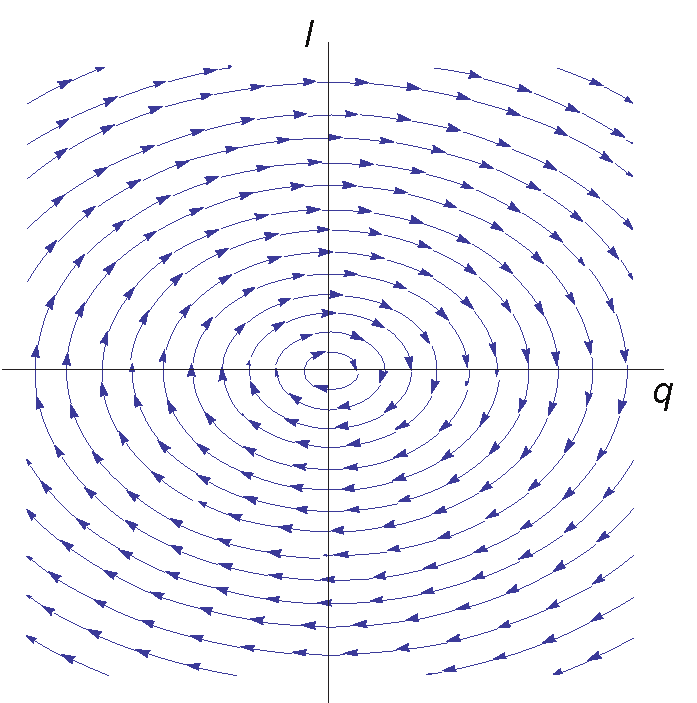
\includegraphics[scale=0.75]{Anh/Trung2.pdf}
        \end{center}
        \item Dấu của điện áp trên diode phụ thuộc vào hướng của dòng điện. Ta có: 
        \[\left\{ \begin{aligned}
        L\Ddot{q} + \frac{q}{C} = {V_d}~~~~~~\text{với}~\Dot{q} < 0 \hfill \\
        L\Ddot {q} + \frac{q}{C} =  - {V_d}~~~~~~\text{với}~\Dot{q}>0 \hfill \\ 
        \end{aligned}  \right. .\]
        Đặt hai biến mới $q_1$, $q_2$ sao cho $q_1=q-CV_d$ và $q_2=q+CV_d$. Ta có:
        \[\left\{ \begin{aligned}
        L\Ddot{q_1} + \frac{q_1}{C} = 0~~~~~~\text{với}~\Dot{q} < 0 \hfill \\
        L\Ddot {q_2} + \frac{q_2}{C} =  0~~~~~~\text{với}~\Dot{q}>0 \hfill \\ 
        \end{aligned}  \right. .\]
        Như vậy, sự ra đời của diode chỉ phục vụ cho việc dịch chuyển các điểm cân bằng tạo thành các quỹ đạo điều hòa đơn giản khác. Với $\Dot{q}>0$, điểm cân bằng là $q_2 = 0$ hoặc $q = -CV_d$, còn với $\Dot{q}<0$ thì $q = CV_d$. Vì vậy, quỹ đạo sẽ bao gồm các nửa hình elipse ở phần trên và phần dưới của biểu đồ $I-q$, có tâm là $q = -CV_d$ đối với nửa trên và tại $q = CV_d$ đối với nửa dưới. Khi quá trình diễn ra liên tục, các nửa hình elipse này sẽ liên kết với nhau tại $I = 0$.
        \begin{center}
            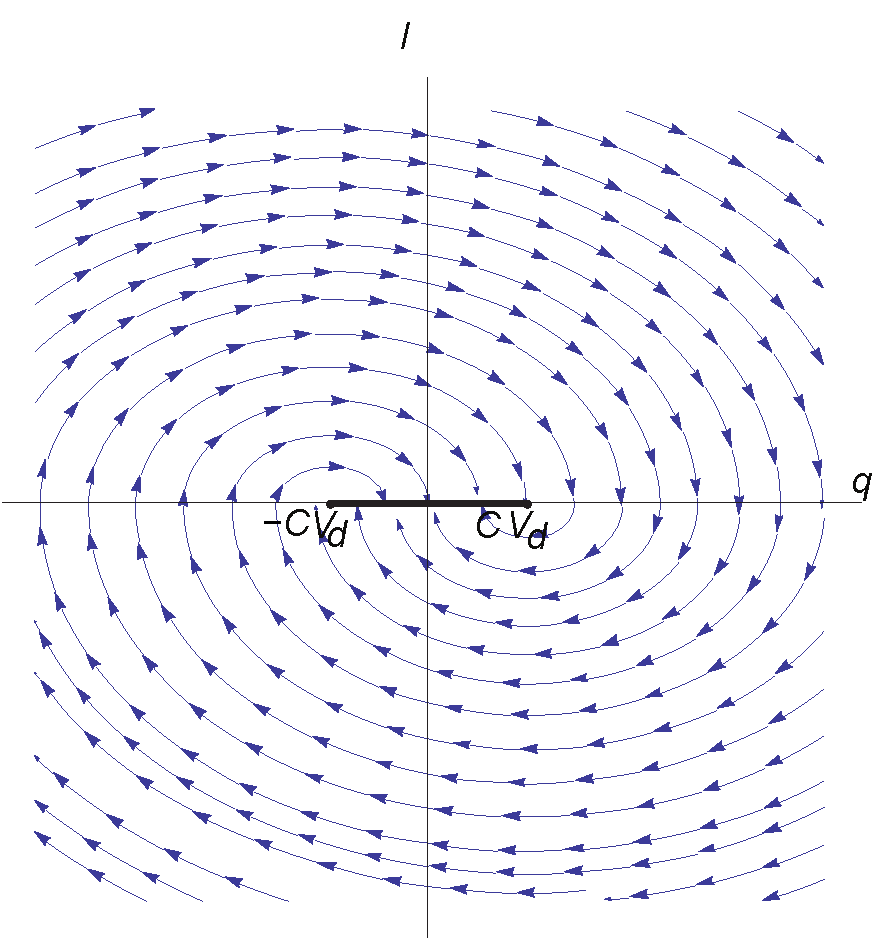
\includegraphics[scale=0.6]{Anh/Trung3.pdf}
        \end{center}
        \item Chúng ta có thể quan sát thấy trên sơ đồ có một “vùng chết” nằm giữa $-CV_d$ và $CV_d$ (với $I = 0$). Nếu một quỹ đạo đạt đến bất kì điểm nào trong đoạn đó, nó sẽ ở đó mãi mãi. Phạm vi của vùng đó là $2CV_d$.
        \item Ở ý này ta sử dụng giản đồ pha.
        \\Giả sử ban đầu tụ điện có điện tích $q_0 \gg CV_d$. Khi đó điện tích ban đầu sẽ dao động theo hướng khác $CV_d$ và sau một nửa chu kỳ: $$q_{T/2}=CV_d-\left(q_0-cV_d)\right)=2CV_d-q_0.$$
        Sau đó nó sẽ thực hiện một nửa dao động còn lại xung quanh $-CV_d$ và điện tích ở cuối dao động là:
        $$q_T=-CV_d-q_0+\left(-CV_d-\left(2CV_d-q_0)\right)\right)=-4CV_d,$$
        và từ đó ta có
        $$\Delta q=-4CV_d.$$
        Lưu ý rằng ta vẫn có thể sử dụng nửa chu kỳ và chu kỳ toàn phần vì dao động luôn xảy ra ở tần số không đổi $\omega=\dfrac{1}{\sqrt{LC}}$. Do đó khoảng thời gian giữa hai lần cực đại chỉ là chu kỳ dao động toàn phần:
        $$T=\dfrac{2\pi}{\omega}.$$
        Một khi $q(t)$ có đạo hàm bằng không trong vùng giới hạn bởi $CV_d$ và $-CV_d$, nó sẽ duy trì trạng thái đó mãi mãi.
    \end{enumerate}
\end{loigiai}


\begin{vd}[Nam châm điện mạnh có điện trở]%APhO 2010 (Taiwan)
Nam châm điện có điện trở là những nam châm được làm bằng những cuộn dây kim loại thông thường như đồng hoặc nhôm. Những nam châm điện có điện trở (sau này ta gọi gọn là nam châm điện) hiện đại có thể cung cấp từ trường không đổi lớn đến hơn $30$ Tesla. \\
Các cuộn dây của chúng thông thường được tạo ra bằng cách ghép hàng trăm đĩa mỏng hình tròn bằng đồng, có khoét nhiều lỗ để làm lạnh, và các tấm cách điện có cùng hình dạng, đặt xen kẽ. Khi một điện áp được đặt vào hai đầu cuộn dây, dòng điện chạy qua các đĩa theo đường xoắn ốc để tạo ra từ trường mạnh ở tâm của nam châm.\\

Trong bài này chúng ta có mục đích khảo sát cuộn dây hình trụ (còn gọi là solenoid) gồm nhiều vòng có thể được dùng như một nam châm để phát ra từ trường mạnh như thế nào. Như thấy trong Hình $1$, tâm của nam châm là ở $O$. Cuộn dây hình trụ của nó gồm $N$ vòng dây đồng có dòng điện $I$, phân bố đồng đều trên tiết diện ngang của dây chạy qua. \\
Đường kính trung bình của cuộn dây là $D$ và chiều dài của nó dọc theo trục $x$ là $l$. Tiết diện ngang của sợi dây là hình chữ nhật có chiều rộng là $a$ và chiều cao là $b$. Các vòng của cuộn dây được quấn sát nhau sao cho mặt phẳng của mỗi vòng có thể xem như vuông góc với trục $x$ và $l=Na$. \\

Dưới đây các số liệu về kích thước của cuộn dây:
\begin{align*}
l&=12,0 \mathrm{~cm}, D=6,0 \mathrm{~cm},\\
a&=2,0 \mathrm{~mm}, b=5,0 \mathrm{~mm}.
 \end{align*}
Khi đánh giá xem liệu một nam châm như vậy có thể tạo ra từ trường cao hay không, có hai thông số giới hạn không thể được bỏ qua. Thứ nhất là độ bền cơ học của cuộn dây để chịu được lực Lorentz lớn khi có dòng điện đi qua cuộn dây tạo ra từ trường. Thứ hai là nhiệt lượng Joule rất lớn toả ra trên sợi dây không được gây ra tăng nhiệt độ quá mức. Chúng ta sẽ khảo sát hai thông số này bằng cách dùng những mô hình đơn giản hóa.
\begin{enumerate}[1)]
    \item \textbf{Từ trường trên trục của cuộn dây}\\
Giả thiết rằng $b \ll D$ và các sợi dây là các dải mỏng có độ rộng $a$. Gọi $O$ là gốc của trục $x$. Hướng của dòng điện chạy qua dây như trong hình bên dưới.
\begin{center}
\tikzset{every picture/.style={line width=0.75pt}} %set default line width to 0.75pt
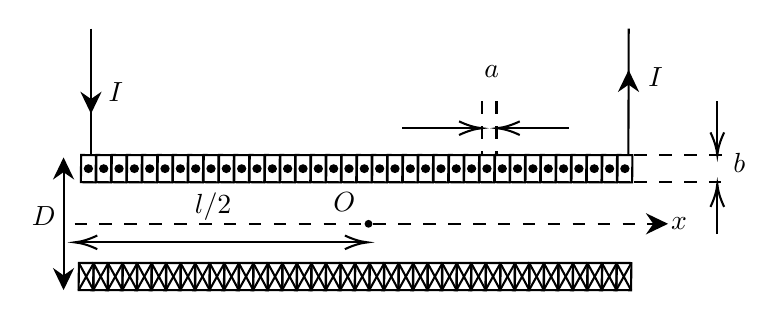
\begin{tikzpicture}[x=0.75pt,y=0.75pt,yscale=-1,xscale=1]
%uncomment if require: \path (0,300); %set diagram left start at 0, and has height of 300
%Shape: Rectangle [id:dp7112702582043747] 
\draw   (180.15,121.95) -- (180.25,108.85) -- (187.35,108.9) -- (187.25,122) -- cycle ;
%Shape: Ellipse [id:dp3338951198805633] 
\draw  [fill={rgb, 255:red, 0; green, 0; blue, 0 }  ,fill opacity=1 ] (182.04,115.43) .. controls (182.04,114.55) and (182.81,113.83) .. (183.75,113.83) .. controls (184.69,113.83) and (185.46,114.55) .. (185.46,115.43) .. controls (185.46,116.31) and (184.69,117.02) .. (183.75,117.02) .. controls (182.81,117.02) and (182.04,116.31) .. (182.04,115.43) -- cycle ;

%Shape: Rectangle [id:dp028506024335763103] 
\draw   (187.53,121.95) -- (187.63,108.85) -- (194.74,108.9) -- (194.64,122) -- cycle ;
%Shape: Ellipse [id:dp3555483150198745] 
\draw  [fill={rgb, 255:red, 0; green, 0; blue, 0 }  ,fill opacity=1 ] (189.43,115.43) .. controls (189.43,114.55) and (190.19,113.83) .. (191.13,113.83) .. controls (192.08,113.83) and (192.84,114.55) .. (192.84,115.43) .. controls (192.84,116.31) and (192.08,117.02) .. (191.13,117.02) .. controls (190.19,117.02) and (189.43,116.31) .. (189.43,115.43) -- cycle ;
%Shape: Rectangle [id:dp7846596217863611] 
\draw   (194.92,121.95) -- (195.02,108.85) -- (202.12,108.9) -- (202.02,122) -- cycle ;
%Shape: Ellipse [id:dp9290969928194137] 
\draw  [fill={rgb, 255:red, 0; green, 0; blue, 0 }  ,fill opacity=1 ] (196.81,115.43) .. controls (196.81,114.55) and (197.58,113.83) .. (198.52,113.83) .. controls (199.46,113.83) and (200.23,114.55) .. (200.23,115.43) .. controls (200.23,116.31) and (199.46,117.02) .. (198.52,117.02) .. controls (197.58,117.02) and (196.81,116.31) .. (196.81,115.43) -- cycle ;


%Shape: Rectangle [id:dp9724587702293661] 
\draw   (202.3,121.95) -- (202.4,108.85) -- (209.51,108.9) -- (209.41,122) -- cycle ;
%Shape: Ellipse [id:dp30621619588689] 
\draw  [fill={rgb, 255:red, 0; green, 0; blue, 0 }  ,fill opacity=1 ] (204.2,115.43) .. controls (204.2,114.55) and (204.96,113.83) .. (205.91,113.83) .. controls (206.85,113.83) and (207.61,114.55) .. (207.61,115.43) .. controls (207.61,116.31) and (206.85,117.02) .. (205.91,117.02) .. controls (204.96,117.02) and (204.2,116.31) .. (204.2,115.43) -- cycle ;

%Shape: Rectangle [id:dp881112043188723] 
\draw   (209.69,121.95) -- (209.79,108.85) -- (216.89,108.9) -- (216.79,122) -- cycle ;
%Shape: Ellipse [id:dp39946646136645925] 
\draw  [fill={rgb, 255:red, 0; green, 0; blue, 0 }  ,fill opacity=1 ] (211.58,115.43) .. controls (211.58,114.55) and (212.35,113.83) .. (213.29,113.83) .. controls (214.23,113.83) and (215,114.55) .. (215,115.43) .. controls (215,116.31) and (214.23,117.02) .. (213.29,117.02) .. controls (212.35,117.02) and (211.58,116.31) .. (211.58,115.43) -- cycle ;

%Shape: Rectangle [id:dp8850466975351513] 
\draw   (217.07,121.95) -- (217.18,108.85) -- (224.28,108.9) -- (224.18,122) -- cycle ;
%Shape: Ellipse [id:dp7335683993198577] 
\draw  [fill={rgb, 255:red, 0; green, 0; blue, 0 }  ,fill opacity=1 ] (218.97,115.43) .. controls (218.97,114.55) and (219.73,113.83) .. (220.68,113.83) .. controls (221.62,113.83) and (222.38,114.55) .. (222.38,115.43) .. controls (222.38,116.31) and (221.62,117.02) .. (220.68,117.02) .. controls (219.73,117.02) and (218.97,116.31) .. (218.97,115.43) -- cycle ;


%Shape: Rectangle [id:dp011164110627033152] 
\draw   (224.46,121.95) -- (224.56,108.85) -- (231.67,108.9) -- (231.56,122) -- cycle ;
%Shape: Ellipse [id:dp5788281664154589] 
\draw  [fill={rgb, 255:red, 0; green, 0; blue, 0 }  ,fill opacity=1 ] (226.35,115.43) .. controls (226.35,114.55) and (227.12,113.83) .. (228.06,113.83) .. controls (229.01,113.83) and (229.77,114.55) .. (229.77,115.43) .. controls (229.77,116.31) and (229.01,117.02) .. (228.06,117.02) .. controls (227.12,117.02) and (226.35,116.31) .. (226.35,115.43) -- cycle ;

%Shape: Rectangle [id:dp13123663982128475] 
\draw   (231.84,121.95) -- (231.95,108.85) -- (239.05,108.9) -- (238.95,122) -- cycle ;
%Shape: Ellipse [id:dp21490954537402496] 
\draw  [fill={rgb, 255:red, 0; green, 0; blue, 0 }  ,fill opacity=1 ] (233.74,115.43) .. controls (233.74,114.55) and (234.5,113.83) .. (235.45,113.83) .. controls (236.39,113.83) and (237.16,114.55) .. (237.16,115.43) .. controls (237.16,116.31) and (236.39,117.02) .. (235.45,117.02) .. controls (234.5,117.02) and (233.74,116.31) .. (233.74,115.43) -- cycle ;

%Shape: Rectangle [id:dp3194367844725694] 
\draw   (239.23,121.95) -- (239.33,108.85) -- (246.44,108.9) -- (246.33,122) -- cycle ;
%Shape: Ellipse [id:dp5546788830074406] 
\draw  [fill={rgb, 255:red, 0; green, 0; blue, 0 }  ,fill opacity=1 ] (241.12,115.43) .. controls (241.12,114.55) and (241.89,113.83) .. (242.83,113.83) .. controls (243.78,113.83) and (244.54,114.55) .. (244.54,115.43) .. controls (244.54,116.31) and (243.78,117.02) .. (242.83,117.02) .. controls (241.89,117.02) and (241.12,116.31) .. (241.12,115.43) -- cycle ;


%Shape: Rectangle [id:dp9887077852251398] 
\draw   (246.61,121.95) -- (246.72,108.85) -- (253.82,108.9) -- (253.72,122) -- cycle ;
%Shape: Ellipse [id:dp29467587578579735] 
\draw  [fill={rgb, 255:red, 0; green, 0; blue, 0 }  ,fill opacity=1 ] (248.51,115.43) .. controls (248.51,114.55) and (249.27,113.83) .. (250.22,113.83) .. controls (251.16,113.83) and (251.93,114.55) .. (251.93,115.43) .. controls (251.93,116.31) and (251.16,117.02) .. (250.22,117.02) .. controls (249.27,117.02) and (248.51,116.31) .. (248.51,115.43) -- cycle ;

%Shape: Rectangle [id:dp46897062738700657] 
\draw   (254,121.95) -- (254.1,108.85) -- (261.21,108.9) -- (261.1,122) -- cycle ;
%Shape: Ellipse [id:dp8225364733033032] 
\draw  [fill={rgb, 255:red, 0; green, 0; blue, 0 }  ,fill opacity=1 ] (255.9,115.43) .. controls (255.9,114.55) and (256.66,113.83) .. (257.6,113.83) .. controls (258.55,113.83) and (259.31,114.55) .. (259.31,115.43) .. controls (259.31,116.31) and (258.55,117.02) .. (257.6,117.02) .. controls (256.66,117.02) and (255.9,116.31) .. (255.9,115.43) -- cycle ;

%Shape: Rectangle [id:dp38295893101591305] 
\draw   (261.39,121.95) -- (261.49,108.85) -- (268.59,108.9) -- (268.49,122) -- cycle ;
%Shape: Ellipse [id:dp5273071025144969] 
\draw  [fill={rgb, 255:red, 0; green, 0; blue, 0 }  ,fill opacity=1 ] (263.28,115.43) .. controls (263.28,114.55) and (264.05,113.83) .. (264.99,113.83) .. controls (265.93,113.83) and (266.7,114.55) .. (266.7,115.43) .. controls (266.7,116.31) and (265.93,117.02) .. (264.99,117.02) .. controls (264.05,117.02) and (263.28,116.31) .. (263.28,115.43) -- cycle ;




%Shape: Rectangle [id:dp784073995306902] 
\draw   (268.77,121.95) -- (268.87,108.85) -- (275.98,108.9) -- (275.87,122) -- cycle ;
%Shape: Ellipse [id:dp013619221540287052] 
\draw  [fill={rgb, 255:red, 0; green, 0; blue, 0 }  ,fill opacity=1 ] (270.67,115.43) .. controls (270.67,114.55) and (271.43,113.83) .. (272.37,113.83) .. controls (273.32,113.83) and (274.08,114.55) .. (274.08,115.43) .. controls (274.08,116.31) and (273.32,117.02) .. (272.37,117.02) .. controls (271.43,117.02) and (270.67,116.31) .. (270.67,115.43) -- cycle ;

%Shape: Rectangle [id:dp9484784833739305] 
\draw   (276.16,121.95) -- (276.26,108.85) -- (283.36,108.9) -- (283.26,122) -- cycle ;
%Shape: Ellipse [id:dp141941792897606] 
\draw  [fill={rgb, 255:red, 0; green, 0; blue, 0 }  ,fill opacity=1 ] (278.05,115.43) .. controls (278.05,114.55) and (278.82,113.83) .. (279.76,113.83) .. controls (280.7,113.83) and (281.47,114.55) .. (281.47,115.43) .. controls (281.47,116.31) and (280.7,117.02) .. (279.76,117.02) .. controls (278.82,117.02) and (278.05,116.31) .. (278.05,115.43) -- cycle ;

%Shape: Rectangle [id:dp6006778057963058] 
\draw   (283.54,121.95) -- (283.64,108.85) -- (290.75,108.9) -- (290.65,122) -- cycle ;
%Shape: Ellipse [id:dp09955296028393701] 
\draw  [fill={rgb, 255:red, 0; green, 0; blue, 0 }  ,fill opacity=1 ] (285.44,115.43) .. controls (285.44,114.55) and (286.2,113.83) .. (287.14,113.83) .. controls (288.09,113.83) and (288.85,114.55) .. (288.85,115.43) .. controls (288.85,116.31) and (288.09,117.02) .. (287.14,117.02) .. controls (286.2,117.02) and (285.44,116.31) .. (285.44,115.43) -- cycle ;


%Shape: Rectangle [id:dp7287708666587742] 
\draw   (290.93,121.95) -- (291.03,108.85) -- (298.13,108.9) -- (298.03,122) -- cycle ;
%Shape: Ellipse [id:dp7591467986810947] 
\draw  [fill={rgb, 255:red, 0; green, 0; blue, 0 }  ,fill opacity=1 ] (292.82,115.43) .. controls (292.82,114.55) and (293.59,113.83) .. (294.53,113.83) .. controls (295.47,113.83) and (296.24,114.55) .. (296.24,115.43) .. controls (296.24,116.31) and (295.47,117.02) .. (294.53,117.02) .. controls (293.59,117.02) and (292.82,116.31) .. (292.82,115.43) -- cycle ;

%Shape: Rectangle [id:dp29665807301733005] 
\draw   (298.31,121.95) -- (298.41,108.85) -- (305.52,108.9) -- (305.42,122) -- cycle ;
%Shape: Ellipse [id:dp00032975296943560384] 
\draw  [fill={rgb, 255:red, 0; green, 0; blue, 0 }  ,fill opacity=1 ] (300.21,115.43) .. controls (300.21,114.55) and (300.97,113.83) .. (301.92,113.83) .. controls (302.86,113.83) and (303.62,114.55) .. (303.62,115.43) .. controls (303.62,116.31) and (302.86,117.02) .. (301.92,117.02) .. controls (300.97,117.02) and (300.21,116.31) .. (300.21,115.43) -- cycle ;

%Shape: Rectangle [id:dp5884814514135553] 
\draw   (305.7,121.95) -- (305.8,108.85) -- (312.9,108.9) -- (312.8,122) -- cycle ;
%Shape: Ellipse [id:dp4752639466274269] 
\draw  [fill={rgb, 255:red, 0; green, 0; blue, 0 }  ,fill opacity=1 ] (307.59,115.43) .. controls (307.59,114.55) and (308.36,113.83) .. (309.3,113.83) .. controls (310.24,113.83) and (311.01,114.55) .. (311.01,115.43) .. controls (311.01,116.31) and (310.24,117.02) .. (309.3,117.02) .. controls (308.36,117.02) and (307.59,116.31) .. (307.59,115.43) -- cycle ;


%Shape: Rectangle [id:dp9356260543152811] 
\draw   (313.08,121.95) -- (313.19,108.85) -- (320.29,108.9) -- (320.19,122) -- cycle ;
%Shape: Ellipse [id:dp6377542837991648] 
\draw  [fill={rgb, 255:red, 0; green, 0; blue, 0 }  ,fill opacity=1 ] (314.98,115.43) .. controls (314.98,114.55) and (315.74,113.83) .. (316.69,113.83) .. controls (317.63,113.83) and (318.39,114.55) .. (318.39,115.43) .. controls (318.39,116.31) and (317.63,117.02) .. (316.69,117.02) .. controls (315.74,117.02) and (314.98,116.31) .. (314.98,115.43) -- cycle ;

%Shape: Rectangle [id:dp1411689651624628] 
\draw   (320.47,121.95) -- (320.57,108.85) -- (327.68,108.9) -- (327.57,122) -- cycle ;
%Shape: Ellipse [id:dp831562196272039] 
\draw  [fill={rgb, 255:red, 0; green, 0; blue, 0 }  ,fill opacity=1 ] (322.36,115.43) .. controls (322.36,114.55) and (323.13,113.83) .. (324.07,113.83) .. controls (325.02,113.83) and (325.78,114.55) .. (325.78,115.43) .. controls (325.78,116.31) and (325.02,117.02) .. (324.07,117.02) .. controls (323.13,117.02) and (322.36,116.31) .. (322.36,115.43) -- cycle ;

%Shape: Rectangle [id:dp889422957038019] 
\draw   (327.85,121.95) -- (327.96,108.85) -- (335.06,108.9) -- (334.96,122) -- cycle ;
%Shape: Ellipse [id:dp5460159483184064] 
\draw  [fill={rgb, 255:red, 0; green, 0; blue, 0 }  ,fill opacity=1 ] (329.75,115.43) .. controls (329.75,114.55) and (330.51,113.83) .. (331.46,113.83) .. controls (332.4,113.83) and (333.17,114.55) .. (333.17,115.43) .. controls (333.17,116.31) and (332.4,117.02) .. (331.46,117.02) .. controls (330.51,117.02) and (329.75,116.31) .. (329.75,115.43) -- cycle ;


%Shape: Rectangle [id:dp9897990727576675] 
\draw   (335.24,121.95) -- (335.34,108.85) -- (342.45,108.9) -- (342.34,122) -- cycle ;
%Shape: Ellipse [id:dp52733387813736] 
\draw  [fill={rgb, 255:red, 0; green, 0; blue, 0 }  ,fill opacity=1 ] (337.13,115.43) .. controls (337.13,114.55) and (337.9,113.83) .. (338.84,113.83) .. controls (339.79,113.83) and (340.55,114.55) .. (340.55,115.43) .. controls (340.55,116.31) and (339.79,117.02) .. (338.84,117.02) .. controls (337.9,117.02) and (337.13,116.31) .. (337.13,115.43) -- cycle ;

%Shape: Rectangle [id:dp725695624099846] 
\draw   (342.62,121.95) -- (342.73,108.85) -- (349.83,108.9) -- (349.73,122) -- cycle ;
%Shape: Ellipse [id:dp7427867514814972] 
\draw  [fill={rgb, 255:red, 0; green, 0; blue, 0 }  ,fill opacity=1 ] (344.52,115.43) .. controls (344.52,114.55) and (345.28,113.83) .. (346.23,113.83) .. controls (347.17,113.83) and (347.94,114.55) .. (347.94,115.43) .. controls (347.94,116.31) and (347.17,117.02) .. (346.23,117.02) .. controls (345.28,117.02) and (344.52,116.31) .. (344.52,115.43) -- cycle ;

%Shape: Rectangle [id:dp3317346861365231] 
\draw   (350.01,121.95) -- (350.11,108.85) -- (357.22,108.9) -- (357.11,122) -- cycle ;
%Shape: Ellipse [id:dp04803915821512861] 
\draw  [fill={rgb, 255:red, 0; green, 0; blue, 0 }  ,fill opacity=1 ] (351.91,115.43) .. controls (351.91,114.55) and (352.67,113.83) .. (353.61,113.83) .. controls (354.56,113.83) and (355.32,114.55) .. (355.32,115.43) .. controls (355.32,116.31) and (354.56,117.02) .. (353.61,117.02) .. controls (352.67,117.02) and (351.91,116.31) .. (351.91,115.43) -- cycle ;




%Shape: Rectangle [id:dp42450437194850266] 
\draw   (357.4,121.95) -- (357.5,108.85) -- (364.6,108.9) -- (364.5,122) -- cycle ;
%Shape: Ellipse [id:dp01674494070503474] 
\draw  [fill={rgb, 255:red, 0; green, 0; blue, 0 }  ,fill opacity=1 ] (359.29,115.43) .. controls (359.29,114.55) and (360.06,113.83) .. (361,113.83) .. controls (361.94,113.83) and (362.71,114.55) .. (362.71,115.43) .. controls (362.71,116.31) and (361.94,117.02) .. (361,117.02) .. controls (360.06,117.02) and (359.29,116.31) .. (359.29,115.43) -- cycle ;

%Shape: Rectangle [id:dp3522070868989857] 
\draw   (364.78,121.95) -- (364.88,108.85) -- (371.99,108.9) -- (371.88,122) -- cycle ;
%Shape: Ellipse [id:dp8092801104277225] 
\draw  [fill={rgb, 255:red, 0; green, 0; blue, 0 }  ,fill opacity=1 ] (366.68,115.43) .. controls (366.68,114.55) and (367.44,113.83) .. (368.38,113.83) .. controls (369.33,113.83) and (370.09,114.55) .. (370.09,115.43) .. controls (370.09,116.31) and (369.33,117.02) .. (368.38,117.02) .. controls (367.44,117.02) and (366.68,116.31) .. (366.68,115.43) -- cycle ;

%Shape: Rectangle [id:dp7884612159751085] 
\draw   (372.17,121.95) -- (372.27,108.85) -- (379.37,108.9) -- (379.27,122) -- cycle ;
%Shape: Ellipse [id:dp9066750814626128] 
\draw  [fill={rgb, 255:red, 0; green, 0; blue, 0 }  ,fill opacity=1 ] (374.06,115.43) .. controls (374.06,114.55) and (374.83,113.83) .. (375.77,113.83) .. controls (376.71,113.83) and (377.48,114.55) .. (377.48,115.43) .. controls (377.48,116.31) and (376.71,117.02) .. (375.77,117.02) .. controls (374.83,117.02) and (374.06,116.31) .. (374.06,115.43) -- cycle ;


%Shape: Rectangle [id:dp38600459532943643] 
\draw   (379.55,121.95) -- (379.65,108.85) -- (386.76,108.9) -- (386.66,122) -- cycle ;
%Shape: Ellipse [id:dp5156570254239508] 
\draw  [fill={rgb, 255:red, 0; green, 0; blue, 0 }  ,fill opacity=1 ] (381.45,115.43) .. controls (381.45,114.55) and (382.21,113.83) .. (383.15,113.83) .. controls (384.1,113.83) and (384.86,114.55) .. (384.86,115.43) .. controls (384.86,116.31) and (384.1,117.02) .. (383.15,117.02) .. controls (382.21,117.02) and (381.45,116.31) .. (381.45,115.43) -- cycle ;

%Shape: Rectangle [id:dp822033913894261] 
\draw   (386.94,121.95) -- (387.04,108.85) -- (394.14,108.9) -- (394.04,122) -- cycle ;
%Shape: Ellipse [id:dp2640157163876288] 
\draw  [fill={rgb, 255:red, 0; green, 0; blue, 0 }  ,fill opacity=1 ] (388.83,115.43) .. controls (388.83,114.55) and (389.6,113.83) .. (390.54,113.83) .. controls (391.48,113.83) and (392.25,114.55) .. (392.25,115.43) .. controls (392.25,116.31) and (391.48,117.02) .. (390.54,117.02) .. controls (389.6,117.02) and (388.83,116.31) .. (388.83,115.43) -- cycle ;

%Shape: Rectangle [id:dp03211620678210958] 
\draw   (394.32,121.95) -- (394.42,108.85) -- (401.53,108.9) -- (401.43,122) -- cycle ;
%Shape: Ellipse [id:dp10653786942375443] 
\draw  [fill={rgb, 255:red, 0; green, 0; blue, 0 }  ,fill opacity=1 ] (396.22,115.43) .. controls (396.22,114.55) and (396.98,113.83) .. (397.93,113.83) .. controls (398.87,113.83) and (399.63,114.55) .. (399.63,115.43) .. controls (399.63,116.31) and (398.87,117.02) .. (397.93,117.02) .. controls (396.98,117.02) and (396.22,116.31) .. (396.22,115.43) -- cycle ;


%Shape: Rectangle [id:dp8168680097809764] 
\draw   (401.71,121.95) -- (401.81,108.85) -- (408.91,108.9) -- (408.81,122) -- cycle ;
%Shape: Ellipse [id:dp5184770831862877] 
\draw  [fill={rgb, 255:red, 0; green, 0; blue, 0 }  ,fill opacity=1 ] (403.6,115.43) .. controls (403.6,114.55) and (404.37,113.83) .. (405.31,113.83) .. controls (406.25,113.83) and (407.02,114.55) .. (407.02,115.43) .. controls (407.02,116.31) and (406.25,117.02) .. (405.31,117.02) .. controls (404.37,117.02) and (403.6,116.31) .. (403.6,115.43) -- cycle ;

%Shape: Rectangle [id:dp6432145807849444] 
\draw   (409.09,121.95) -- (409.2,108.85) -- (416.3,108.9) -- (416.2,122) -- cycle ;
%Shape: Ellipse [id:dp41294015300693454] 
\draw  [fill={rgb, 255:red, 0; green, 0; blue, 0 }  ,fill opacity=1 ] (410.99,115.43) .. controls (410.99,114.55) and (411.75,113.83) .. (412.7,113.83) .. controls (413.64,113.83) and (414.4,114.55) .. (414.4,115.43) .. controls (414.4,116.31) and (413.64,117.02) .. (412.7,117.02) .. controls (411.75,117.02) and (410.99,116.31) .. (410.99,115.43) -- cycle ;

%Shape: Rectangle [id:dp35183153364110153] 
\draw   (416.48,121.95) -- (416.58,108.85) -- (423.69,108.9) -- (423.58,122) -- cycle ;
%Shape: Ellipse [id:dp21391903391699074] 
\draw  [fill={rgb, 255:red, 0; green, 0; blue, 0 }  ,fill opacity=1 ] (418.37,115.43) .. controls (418.37,114.55) and (419.14,113.83) .. (420.08,113.83) .. controls (421.03,113.83) and (421.79,114.55) .. (421.79,115.43) .. controls (421.79,116.31) and (421.03,117.02) .. (420.08,117.02) .. controls (419.14,117.02) and (418.37,116.31) .. (418.37,115.43) -- cycle ;
%Shape: Rectangle [id:dp8052015452934143] 
\draw   (423.86,121.95) -- (423.97,108.85) -- (431.07,108.9) -- (430.97,122) -- cycle ;
%Shape: Ellipse [id:dp9191916804986576] 
\draw  [fill={rgb, 255:red, 0; green, 0; blue, 0 }  ,fill opacity=1 ] (425.76,115.43) .. controls (425.76,114.55) and (426.52,113.83) .. (427.47,113.83) .. controls (428.41,113.83) and (429.18,114.55) .. (429.18,115.43) .. controls (429.18,116.31) and (428.41,117.02) .. (427.47,117.02) .. controls (426.52,117.02) and (425.76,116.31) .. (425.76,115.43) -- cycle ;

%Shape: Rectangle [id:dp5944503155233724] 
\draw   (431.25,121.95) -- (431.35,108.85) -- (438.46,108.9) -- (438.35,122) -- cycle ;
%Shape: Ellipse [id:dp4067424083970931] 
\draw  [fill={rgb, 255:red, 0; green, 0; blue, 0 }  ,fill opacity=1 ] (433.14,115.43) .. controls (433.14,114.55) and (433.91,113.83) .. (434.85,113.83) .. controls (435.8,113.83) and (436.56,114.55) .. (436.56,115.43) .. controls (436.56,116.31) and (435.8,117.02) .. (434.85,117.02) .. controls (433.91,117.02) and (433.14,116.31) .. (433.14,115.43) -- cycle ;

%Shape: Rectangle [id:dp3093602824130668] 
\draw   (438.63,121.95) -- (438.74,108.85) -- (445.84,108.9) -- (445.74,122) -- cycle ;
%Shape: Ellipse [id:dp6433098435754134] 
\draw  [fill={rgb, 255:red, 0; green, 0; blue, 0 }  ,fill opacity=1 ] (440.53,115.43) .. controls (440.53,114.55) and (441.29,113.83) .. (442.24,113.83) .. controls (443.18,113.83) and (443.95,114.55) .. (443.95,115.43) .. controls (443.95,116.31) and (443.18,117.02) .. (442.24,117.02) .. controls (441.29,117.02) and (440.53,116.31) .. (440.53,115.43) -- cycle ;
%Shape: Rectangle [id:dp4500570570513234] 
\draw   (179.06,173.95) -- (179.16,160.85) -- (186.34,160.9) -- (186.23,174) -- cycle ;
%Straight Lines [id:da40625266460131937] 
\draw    (179.16,160.85) -- (186.23,174) ;
%Straight Lines [id:da18787088993541978] 
\draw    (186.34,160.9) -- (179.06,173.95) ;

%Shape: Rectangle [id:dp4325467058988054] 
\draw   (186.06,173.95) -- (186.16,160.85) -- (193.34,160.9) -- (193.23,174) -- cycle ;
%Straight Lines [id:da5147676972043498] 
\draw    (186.16,160.85) -- (193.23,174) ;
%Straight Lines [id:da8417179321174847] 
\draw    (193.34,160.9) -- (186.06,173.95) ;
%Shape: Rectangle [id:dp6665550349790494] 
\draw   (193.06,173.95) -- (193.16,160.85) -- (200.34,160.9) -- (200.23,174) -- cycle ;
%Straight Lines [id:da4806525093998497] 
\draw    (193.16,160.85) -- (200.23,174) ;
%Straight Lines [id:da3731763781263795] 
\draw    (200.34,160.9) -- (193.06,173.95) ;

%Shape: Rectangle [id:dp42494674280831435] 
\draw   (200.06,173.95) -- (200.16,160.85) -- (207.34,160.9) -- (207.23,174) -- cycle ;
%Straight Lines [id:da134258348341728] 
\draw    (200.16,160.85) -- (207.23,174) ;
%Straight Lines [id:da36141604129807003] 
\draw    (207.34,160.9) -- (200.06,173.95) ;
%Shape: Rectangle [id:dp3256425944072524] 
\draw   (207.06,173.95) -- (207.16,160.85) -- (214.34,160.9) -- (214.23,174) -- cycle ;
%Straight Lines [id:da37176518579844264] 
\draw    (207.16,160.85) -- (214.23,174) ;
%Straight Lines [id:da15918698372562867] 
\draw    (214.34,160.9) -- (207.06,173.95) ;

%Shape: Rectangle [id:dp3994081441878239] 
\draw   (214.06,173.95) -- (214.16,160.85) -- (221.34,160.9) -- (221.23,174) -- cycle ;
%Straight Lines [id:da9398829129746036] 
\draw    (214.16,160.85) -- (221.23,174) ;
%Straight Lines [id:da23700468283234544] 
\draw    (221.34,160.9) -- (214.06,173.95) ;


%Shape: Rectangle [id:dp6251615265933044] 
\draw   (221.06,173.95) -- (221.16,160.85) -- (228.34,160.9) -- (228.23,174) -- cycle ;
%Straight Lines [id:da20036953230592414] 
\draw    (221.16,160.85) -- (228.23,174) ;
%Straight Lines [id:da41255606890342145] 
\draw    (228.34,160.9) -- (221.06,173.95) ;

%Shape: Rectangle [id:dp47616886390663316] 
\draw   (228.06,173.95) -- (228.16,160.85) -- (235.34,160.9) -- (235.23,174) -- cycle ;
%Straight Lines [id:da34849367261456055] 
\draw    (228.16,160.85) -- (235.23,174) ;
%Straight Lines [id:da03523732887148279] 
\draw    (235.34,160.9) -- (228.06,173.95) ;

%Shape: Rectangle [id:dp19067595157342854] 
\draw   (235.06,173.95) -- (235.16,160.85) -- (242.34,160.9) -- (242.23,174) -- cycle ;
%Straight Lines [id:da32478107063564754] 
\draw    (235.16,160.85) -- (242.23,174) ;
%Straight Lines [id:da3286014335035734] 
\draw    (242.34,160.9) -- (235.06,173.95) ;

%Shape: Rectangle [id:dp5245989805903607] 
\draw   (242.06,173.95) -- (242.16,160.85) -- (249.34,160.9) -- (249.23,174) -- cycle ;
%Straight Lines [id:da961416414924577] 
\draw    (242.16,160.85) -- (249.23,174) ;
%Straight Lines [id:da9745930078958432] 
\draw    (249.34,160.9) -- (242.06,173.95) ;


%Shape: Rectangle [id:dp5751636813361185] 
\draw   (249.06,173.95) -- (249.16,160.85) -- (256.34,160.9) -- (256.23,174) -- cycle ;
%Straight Lines [id:da3217654102132803] 
\draw    (249.16,160.85) -- (256.23,174) ;
%Straight Lines [id:da9220913921976156] 
\draw    (256.34,160.9) -- (249.06,173.95) ;

%Shape: Rectangle [id:dp15983781540062947] 
\draw   (256.06,173.95) -- (256.16,160.85) -- (263.34,160.9) -- (263.23,174) -- cycle ;
%Straight Lines [id:da2140887225636865] 
\draw    (256.16,160.85) -- (263.23,174) ;
%Straight Lines [id:da2859353699918723] 
\draw    (263.34,160.9) -- (256.06,173.95) ;



%Shape: Rectangle [id:dp15984452442185926] 
\draw   (263.06,173.95) -- (263.16,160.85) -- (270.34,160.9) -- (270.23,174) -- cycle ;
%Straight Lines [id:da4110719136821098] 
\draw    (263.16,160.85) -- (270.23,174) ;
%Straight Lines [id:da26052700975351817] 
\draw    (270.34,160.9) -- (263.06,173.95) ;

%Shape: Rectangle [id:dp6566474198918585] 
\draw   (270.06,173.95) -- (270.16,160.85) -- (277.34,160.9) -- (277.23,174) -- cycle ;
%Straight Lines [id:da28372319029960713] 
\draw    (270.16,160.85) -- (277.23,174) ;
%Straight Lines [id:da8573144369125063] 
\draw    (277.34,160.9) -- (270.06,173.95) ;


%Shape: Rectangle [id:dp2769638883772084] 
\draw   (277.06,173.95) -- (277.16,160.85) -- (284.34,160.9) -- (284.23,174) -- cycle ;
%Straight Lines [id:da4320871028995078] 
\draw    (277.16,160.85) -- (284.23,174) ;
%Straight Lines [id:da7269875737873256] 
\draw    (284.34,160.9) -- (277.06,173.95) ;

%Shape: Rectangle [id:dp49533982823384426] 
\draw   (284.06,173.95) -- (284.16,160.85) -- (291.34,160.9) -- (291.23,174) -- cycle ;
%Straight Lines [id:da6090040044011437] 
\draw    (284.16,160.85) -- (291.23,174) ;
%Straight Lines [id:da6091351527578889] 
\draw    (291.34,160.9) -- (284.06,173.95) ;




%Shape: Rectangle [id:dp6882053419001805] 
\draw   (291.06,173.95) -- (291.16,160.85) -- (298.34,160.9) -- (298.23,174) -- cycle ;
%Straight Lines [id:da3086131390592649] 
\draw    (291.16,160.85) -- (298.23,174) ;
%Straight Lines [id:da1671891417612409] 
\draw    (298.34,160.9) -- (291.06,173.95) ;

%Shape: Rectangle [id:dp3844713554864301] 
\draw   (298.06,173.95) -- (298.16,160.85) -- (305.34,160.9) -- (305.23,174) -- cycle ;
%Straight Lines [id:da9809181313237885] 
\draw    (298.16,160.85) -- (305.23,174) ;
%Straight Lines [id:da12067399015099456] 
\draw    (305.34,160.9) -- (298.06,173.95) ;


%Shape: Rectangle [id:dp09660124994154662] 
\draw   (305.06,173.95) -- (305.16,160.85) -- (312.34,160.9) -- (312.23,174) -- cycle ;
%Straight Lines [id:da23391988796153762] 
\draw    (305.16,160.85) -- (312.23,174) ;
%Straight Lines [id:da030740420735130614] 
\draw    (312.34,160.9) -- (305.06,173.95) ;

%Shape: Rectangle [id:dp674441868316983] 
\draw   (312.06,173.95) -- (312.16,160.85) -- (319.34,160.9) -- (319.23,174) -- cycle ;
%Straight Lines [id:da808857912590329] 
\draw    (312.16,160.85) -- (319.23,174) ;
%Straight Lines [id:da5955291111145252] 
\draw    (319.34,160.9) -- (312.06,173.95) ;



%Shape: Rectangle [id:dp7235119922972411] 
\draw   (319.06,173.95) -- (319.16,160.85) -- (326.34,160.9) -- (326.23,174) -- cycle ;
%Straight Lines [id:da6868703727152485] 
\draw    (319.16,160.85) -- (326.23,174) ;
%Straight Lines [id:da32489055181574666] 
\draw    (326.34,160.9) -- (319.06,173.95) ;

%Shape: Rectangle [id:dp7184067120736121] 
\draw   (326.06,173.95) -- (326.16,160.85) -- (333.34,160.9) -- (333.23,174) -- cycle ;
%Straight Lines [id:da3604883540635465] 
\draw    (326.16,160.85) -- (333.23,174) ;
%Straight Lines [id:da09742421672475432] 
\draw    (333.34,160.9) -- (326.06,173.95) ;


%Shape: Rectangle [id:dp6079758585573741] 
\draw   (333.06,173.95) -- (333.16,160.85) -- (340.34,160.9) -- (340.23,174) -- cycle ;
%Straight Lines [id:da5347028805170088] 
\draw    (333.16,160.85) -- (340.23,174) ;
%Straight Lines [id:da8422657200640619] 
\draw    (340.34,160.9) -- (333.06,173.95) ;

%Shape: Rectangle [id:dp20488235707161762] 
\draw   (340.06,173.95) -- (340.16,160.85) -- (347.34,160.9) -- (347.23,174) -- cycle ;
%Straight Lines [id:da17763451342370007] 
\draw    (340.16,160.85) -- (347.23,174) ;
%Straight Lines [id:da7248086984737857] 
\draw    (347.34,160.9) -- (340.06,173.95) ;



%Shape: Rectangle [id:dp2629321914496321] 
\draw   (347.06,173.95) -- (347.16,160.85) -- (354.34,160.9) -- (354.23,174) -- cycle ;
%Straight Lines [id:da6488045820160981] 
\draw    (347.16,160.85) -- (354.23,174) ;
%Straight Lines [id:da8196087287107547] 
\draw    (354.34,160.9) -- (347.06,173.95) ;

%Shape: Rectangle [id:dp5638281747253037] 
\draw   (354.06,173.95) -- (354.16,160.85) -- (361.34,160.9) -- (361.23,174) -- cycle ;
%Straight Lines [id:da28521897455028866] 
\draw    (354.16,160.85) -- (361.23,174) ;
%Straight Lines [id:da19012165260693004] 
\draw    (361.34,160.9) -- (354.06,173.95) ;


%Shape: Rectangle [id:dp09125154066341357] 
\draw   (361.06,173.95) -- (361.16,160.85) -- (368.34,160.9) -- (368.23,174) -- cycle ;
%Straight Lines [id:da22633566243480363] 
\draw    (361.16,160.85) -- (368.23,174) ;
%Straight Lines [id:da017531305380509288] 
\draw    (368.34,160.9) -- (361.06,173.95) ;

%Shape: Rectangle [id:dp3594876506577861] 
\draw   (368.06,173.95) -- (368.16,160.85) -- (375.34,160.9) -- (375.23,174) -- cycle ;
%Straight Lines [id:da5735427887107543] 
\draw    (368.16,160.85) -- (375.23,174) ;
%Straight Lines [id:da32558479740425295] 
\draw    (375.34,160.9) -- (368.06,173.95) ;



%Shape: Rectangle [id:dp6160129635069435] 
\draw   (375.06,173.95) -- (375.16,160.85) -- (382.34,160.9) -- (382.23,174) -- cycle ;
%Straight Lines [id:da18228486282733514] 
\draw    (375.16,160.85) -- (382.23,174) ;
%Straight Lines [id:da8223113338216818] 
\draw    (382.34,160.9) -- (375.06,173.95) ;

%Shape: Rectangle [id:dp9978569121245916] 
\draw   (382.06,173.95) -- (382.16,160.85) -- (389.34,160.9) -- (389.23,174) -- cycle ;
%Straight Lines [id:da6435723893249009] 
\draw    (382.16,160.85) -- (389.23,174) ;
%Straight Lines [id:da32916005292625083] 
\draw    (389.34,160.9) -- (382.06,173.95) ;


%Shape: Rectangle [id:dp9192366414171145] 
\draw   (389.06,173.95) -- (389.16,160.85) -- (396.34,160.9) -- (396.23,174) -- cycle ;
%Straight Lines [id:da8194757202727903] 
\draw    (389.16,160.85) -- (396.23,174) ;
%Straight Lines [id:da369894572124559] 
\draw    (396.34,160.9) -- (389.06,173.95) ;

%Shape: Rectangle [id:dp8339770088814564] 
\draw   (396.06,173.95) -- (396.16,160.85) -- (403.34,160.9) -- (403.23,174) -- cycle ;
%Straight Lines [id:da746423457027386] 
\draw    (396.16,160.85) -- (403.23,174) ;
%Straight Lines [id:da6993056754402005] 
\draw    (403.34,160.9) -- (396.06,173.95) ;





%Shape: Rectangle [id:dp7236839368947763] 
\draw   (403.06,173.95) -- (403.16,160.85) -- (410.34,160.9) -- (410.23,174) -- cycle ;
%Straight Lines [id:da8786499357131579] 
\draw    (403.16,160.85) -- (410.23,174) ;
%Straight Lines [id:da2682904482226657] 
\draw    (410.34,160.9) -- (403.06,173.95) ;

%Shape: Rectangle [id:dp6089797136712847] 
\draw   (410.06,173.95) -- (410.16,160.85) -- (417.34,160.9) -- (417.23,174) -- cycle ;
%Straight Lines [id:da9632799437797668] 
\draw    (410.16,160.85) -- (417.23,174) ;
%Straight Lines [id:da19697634125974028] 
\draw    (417.34,160.9) -- (410.06,173.95) ;


%Shape: Rectangle [id:dp5515886144534714] 
\draw   (417.06,173.95) -- (417.16,160.85) -- (424.34,160.9) -- (424.23,174) -- cycle ;
%Straight Lines [id:da6368801592408003] 
\draw    (417.16,160.85) -- (424.23,174) ;
%Straight Lines [id:da6363278253993598] 
\draw    (424.34,160.9) -- (417.06,173.95) ;

%Shape: Rectangle [id:dp9971356550887577] 
\draw   (424.06,173.95) -- (424.16,160.85) -- (431.34,160.9) -- (431.23,174) -- cycle ;
%Straight Lines [id:da5844379967942365] 
\draw    (424.16,160.85) -- (431.23,174) ;
%Straight Lines [id:da7902201274332762] 
\draw    (431.34,160.9) -- (424.06,173.95) ;


%Shape: Rectangle [id:dp7197048614654172] 
\draw   (431.06,173.95) -- (431.16,160.85) -- (438.34,160.9) -- (438.23,174) -- cycle ;
%Straight Lines [id:da07608131854628042] 
\draw    (431.16,160.85) -- (438.23,174) ;
%Straight Lines [id:da409418423453491] 
\draw    (438.34,160.9) -- (431.06,173.95) ;

%Shape: Rectangle [id:dp790299159662829] 
\draw   (438.06,173.95) -- (438.16,160.85) -- (445.34,160.9) -- (445.23,174) -- cycle ;
%Straight Lines [id:da8905664662233008] 
\draw    (438.16,160.85) -- (445.23,174) ;
%Straight Lines [id:da8777132345983735] 
\draw    (445.34,160.9) -- (438.06,173.95) ;


%Straight Lines [id:da7296224435771693] 
\draw  [dash pattern={on 4.5pt off 4.5pt}]  (177.1,142) -- (460.03,142) ;
\draw [shift={(463.03,142)}, rotate = 180] [fill={rgb, 255:red, 0; green, 0; blue, 0 }  ][line width=0.08]  [draw opacity=0] (10.72,-5.15) -- (0,0) -- (10.72,5.15) -- (7.12,0) -- cycle    ;
%Straight Lines [id:da8720938481462964] 
\draw    (185,48) -- (185,86) ;
\draw [shift={(185,89)}, rotate = 270] [fill={rgb, 255:red, 0; green, 0; blue, 0 }  ][line width=0.08]  [draw opacity=0] (10.72,-5.15) -- (0,0) -- (10.72,5.15) -- (7.12,0) -- cycle    ;
%Straight Lines [id:da6907872806919281] 
\draw    (185,82) -- (185,108.85) ;

%Straight Lines [id:da5572396234121316] 
\draw    (443.92,108.85) -- (444.02,70.85) ;
\draw [shift={(444.03,67.85)}, rotate = 450.16] [fill={rgb, 255:red, 0; green, 0; blue, 0 }  ][line width=0.08]  [draw opacity=0] (10.72,-5.15) -- (0,0) -- (10.72,5.15) -- (7.12,0) -- cycle    ;
%Straight Lines [id:da7687623210079318] 
\draw    (444.01,74.85) -- (444.08,48) ;

%Straight Lines [id:da40679695822258843] 
\draw  [dash pattern={on 4.5pt off 4.5pt}]  (373.27,83) -- (373.27,108.85) ;
%Straight Lines [id:da4305574450084835] 
\draw  [dash pattern={on 4.5pt off 4.5pt}]  (380.37,83.05) -- (380.37,108.9) ;
%Straight Lines [id:da3371320583572225] 
\draw    (335,95.93) -- (371.27,95.93) ;
\draw [shift={(373.27,95.93)}, rotate = 180] [color={rgb, 255:red, 0; green, 0; blue, 0 }  ][line width=0.75]    (10.93,-3.29) .. controls (6.95,-1.4) and (3.31,-0.3) .. (0,0) .. controls (3.31,0.3) and (6.95,1.4) .. (10.93,3.29)   ;
%Straight Lines [id:da7113372851252481] 
\draw    (415.28,95.93) -- (382.65,95.93) ;
\draw [shift={(380.65,95.93)}, rotate = 360] [color={rgb, 255:red, 0; green, 0; blue, 0 }  ][line width=0.75]    (10.93,-3.29) .. controls (6.95,-1.4) and (3.31,-0.3) .. (0,0) .. controls (3.31,0.3) and (6.95,1.4) .. (10.93,3.29)   ;
%Straight Lines [id:da1668456872781937] 
\draw    (171.79,170.95) -- (171.79,113) ;
\draw [shift={(171.79,110)}, rotate = 450] [fill={rgb, 255:red, 0; green, 0; blue, 0 }  ][line width=0.08]  [draw opacity=0] (10.72,-5.15) -- (0,0) -- (10.72,5.15) -- (7.12,0) -- cycle    ;
\draw [shift={(171.79,173.95)}, rotate = 270] [fill={rgb, 255:red, 0; green, 0; blue, 0 }  ][line width=0.08]  [draw opacity=0] (10.72,-5.15) -- (0,0) -- (10.72,5.15) -- (7.12,0) -- cycle    ;
%Straight Lines [id:da9142893613693474] 
\draw  [dash pattern={on 4.5pt off 4.5pt}]  (446.74,122) -- (492.57,122) ;
%Straight Lines [id:da333519531602262] 
\draw  [dash pattern={on 4.5pt off 4.5pt}]  (446.84,108.9) -- (492.67,108.9) ;
%Straight Lines [id:da5598803394969128] 
\draw    (486.76,83) -- (486.76,106.9) ;
\draw [shift={(486.76,108.9)}, rotate = 270] [color={rgb, 255:red, 0; green, 0; blue, 0 }  ][line width=0.75]    (10.93,-3.29) .. controls (6.95,-1.4) and (3.31,-0.3) .. (0,0) .. controls (3.31,0.3) and (6.95,1.4) .. (10.93,3.29)   ;
%Straight Lines [id:da6334677440312976] 
\draw    (486.76,147) -- (486.76,124.9) ;
\draw [shift={(486.76,122.9)}, rotate = 450] [color={rgb, 255:red, 0; green, 0; blue, 0 }  ][line width=0.75]    (10.93,-3.29) .. controls (6.95,-1.4) and (3.31,-0.3) .. (0,0) .. controls (3.31,0.3) and (6.95,1.4) .. (10.93,3.29)   ;
%Shape: Circle [id:dp9238447922347451] 
\draw  [fill={rgb, 255:red, 0; green, 0; blue, 0 }  ,fill opacity=1 ] (317.37,142) .. controls (317.37,141.25) and (317.97,140.65) .. (318.72,140.65) .. controls (319.46,140.65) and (320.07,141.25) .. (320.07,142) .. controls (320.07,142.75) and (319.46,143.35) .. (318.72,143.35) .. controls (317.97,143.35) and (317.37,142.75) .. (317.37,142) -- cycle ;
%Straight Lines [id:da748231115663523] 
\draw    (179.1,150.93) -- (316.27,150.93) ;
\draw [shift={(318.27,150.93)}, rotate = 180] [color={rgb, 255:red, 0; green, 0; blue, 0 }  ][line width=0.75]    (10.93,-3.29) .. controls (6.95,-1.4) and (3.31,-0.3) .. (0,0) .. controls (3.31,0.3) and (6.95,1.4) .. (10.93,3.29)   ;
\draw [shift={(177.1,150.93)}, rotate = 0] [color={rgb, 255:red, 0; green, 0; blue, 0 }  ][line width=0.75]    (10.93,-3.29) .. controls (6.95,-1.4) and (3.31,-0.3) .. (0,0) .. controls (3.31,0.3) and (6.95,1.4) .. (10.93,3.29)   ;

% Text Node
\draw (192,72.4) node [anchor=north west][inner sep=0.75pt]    {$I$};
% Text Node
\draw (452,65.4) node [anchor=north west][inner sep=0.75pt]    {$I$};
% Text Node
\draw (373,64.4) node [anchor=north west][inner sep=0.75pt]    {$a$};
% Text Node
\draw (155,132.4) node [anchor=north west][inner sep=0.75pt]    {$D$};
% Text Node
\draw (493,106.4) node [anchor=north west][inner sep=0.75pt]    {$b$};
% Text Node
\draw (233.56,125.4) node [anchor=north west][inner sep=0.75pt]  [rotate=-0.12]  {$l/2$};
% Text Node
\draw (300.31,125.35) node [anchor=north west][inner sep=0.75pt]    {$O$};
% Text Node
\draw (463,137.4) node [anchor=north west][inner sep=0.75pt]    {$x$};


\end{tikzpicture}
\\ Hình 1
\end{center}
\begin{enumerate}[a)]
    \item Hãy xác định thành phần theo trục $x$ của từ trường $B(x)$ trên trục của cuộn dây theo $x$ khi dòng điện không đổi $I$ chạy qua cuộn. 
    \item Hãy xác định dòng điện không đổi $I_{0}$ qua cuộn dây nếu $B(0)$ bằng $10,0 \mathrm{~T}$. Sử dụng các dữ liệu được cho ở trên để tính toán trong phần này.
\end{enumerate}
\item \textbf{Giới hạn trên của dòng điện }\\
Trong phần này, chúng ta giả sử độ dài của cuộn dây là vô hạn và $b \ll D$. Xét một vòng của cuộn dây ở vị trí $x=0$. Từ trường tác dụng lực Lorentz lên dòng điện chạy qua các vòng dây. Vậy, như trên Hình $2$, đoạn dây độ dài $\Delta{s}$ chịu lực pháp tuyến $\Delta{F_n}$ có xu hướng làm cho vòng dây dãn rộng ra.
\begin{enumerate}[a)]
    \item Giả sử rằng, khi dòng điện là $I$, đường kính trung bình của cuộn dây đã dãn ra và được giữ ở giá trị không đổi $D'$ lớn hơn $D$, như hình dưới đây.
    \begin{center}
\tikzset{every picture/.style={line width=0.75pt}} %set default line width to 0.75pt
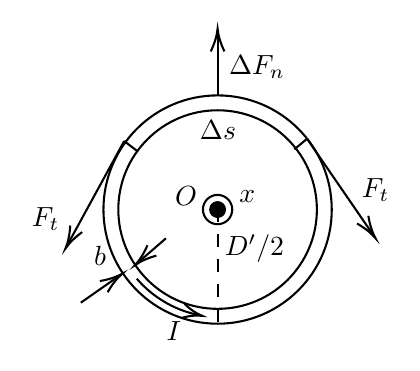
\begin{tikzpicture}[x=0.75pt,y=0.75pt,yscale=-1,xscale=1]
%uncomment if require: \path (0,300); %set diagram left start at 0, and has height of 300

%Shape: Circle [id:dp8834988581353049] 
\draw   (165.17,115) .. controls (165.17,88.58) and (186.58,67.17) .. (213,67.17) .. controls (239.42,67.17) and (260.83,88.58) .. (260.83,115) .. controls (260.83,141.42) and (239.42,162.83) .. (213,162.83) .. controls (186.58,162.83) and (165.17,141.42) .. (165.17,115) -- cycle ;
%Shape: Circle [id:dp9516308900374016] 
\draw   (158,115) .. controls (158,84.62) and (182.62,60) .. (213,60) .. controls (243.38,60) and (268,84.62) .. (268,115) .. controls (268,145.38) and (243.38,170) .. (213,170) .. controls (182.62,170) and (158,145.38) .. (158,115) -- cycle ;
%Straight Lines [id:da4223301871069537] 
\draw    (168,82) -- (174.65,87.09) ;
%Straight Lines [id:da7547159000679459] 
\draw    (168,82) -- (140.61,132.12) ;
\draw [shift={(139.65,133.87)}, rotate = 298.65999999999997] [color={rgb, 255:red, 0; green, 0; blue, 0 }  ][line width=0.75]    (10.93,-3.29) .. controls (6.95,-1.4) and (3.31,-0.3) .. (0,0) .. controls (3.31,0.3) and (6.95,1.4) .. (10.93,3.29)   ;
%Straight Lines [id:da9240376259820594] 
\draw    (250,86) -- (256.11,80.87) ;
%Straight Lines [id:da894481673132922] 
\draw    (256.11,80.87) -- (287.98,127.22) ;
\draw [shift={(289.11,128.87)}, rotate = 235.49] [color={rgb, 255:red, 0; green, 0; blue, 0 }  ][line width=0.75]    (10.93,-3.29) .. controls (6.95,-1.4) and (3.31,-0.3) .. (0,0) .. controls (3.31,0.3) and (6.95,1.4) .. (10.93,3.29)   ;
%Straight Lines [id:da3410932148713175] 
\draw    (213,60) -- (213,29.87) ;
\draw [shift={(213,27.87)}, rotate = 450] [color={rgb, 255:red, 0; green, 0; blue, 0 }  ][line width=0.75]    (10.93,-3.29) .. controls (6.95,-1.4) and (3.31,-0.3) .. (0,0) .. controls (3.31,0.3) and (6.95,1.4) .. (10.93,3.29)   ;
%Shape: Circle [id:dp3062913686317801] 
\draw  [fill={rgb, 255:red, 0; green, 0; blue, 0 }  ,fill opacity=1 ] (209.44,115) .. controls (209.44,113.03) and (211.03,111.44) .. (213,111.44) .. controls (214.97,111.44) and (216.56,113.03) .. (216.56,115) .. controls (216.56,116.97) and (214.97,118.56) .. (213,118.56) .. controls (211.03,118.56) and (209.44,116.97) .. (209.44,115) -- cycle ;
%Shape: Circle [id:dp3444366281443707] 
\draw   (205.94,115) .. controls (205.94,111.1) and (209.1,107.94) .. (213,107.94) .. controls (216.9,107.94) and (220.06,111.1) .. (220.06,115) .. controls (220.06,118.9) and (216.9,122.06) .. (213,122.06) .. controls (209.1,122.06) and (205.94,118.9) .. (205.94,115) -- cycle ;
%Straight Lines [id:da7340652094458986] 
\draw    (147.11,159.87) -- (165.47,147.02) ;
\draw [shift={(167.11,145.87)}, rotate = 505.01] [color={rgb, 255:red, 0; green, 0; blue, 0 }  ][line width=0.75]    (10.93,-3.29) .. controls (6.95,-1.4) and (3.31,-0.3) .. (0,0) .. controls (3.31,0.3) and (6.95,1.4) .. (10.93,3.29)   ;
%Straight Lines [id:da5172572316609994] 
\draw    (188.11,128.87) -- (174.62,140.56) ;
\draw [shift={(173.11,141.87)}, rotate = 319.09000000000003] [color={rgb, 255:red, 0; green, 0; blue, 0 }  ][line width=0.75]    (10.93,-3.29) .. controls (6.95,-1.4) and (3.31,-0.3) .. (0,0) .. controls (3.31,0.3) and (6.95,1.4) .. (10.93,3.29)   ;
%Straight Lines [id:da774902533748078] 
\draw  [dash pattern={on 4.5pt off 4.5pt}]  (213,115) -- (213,170) ;
%Shape: Arc [id:dp774835564057123] 
\draw  [draw opacity=0] (202.95,165.61) .. controls (191.52,163.08) and (181.46,156.88) .. (174.07,148.32) -- (214.56,113.44) -- cycle ; \draw   (202.95,165.61) .. controls (191.52,163.08) and (181.46,156.88) .. (174.07,148.32) ;
\draw   (197.11,160.4) .. controls (199.75,163.11) and (202.58,165.04) .. (205.6,166.21) .. controls (202.39,165.81) and (198.97,166.18) .. (195.37,167.32) ;

% Text Node
\draw (122,112.4) node [anchor=north west][inner sep=0.75pt]    {$F_{t}$};
% Text Node
\draw (281,98.4) node [anchor=north west][inner sep=0.75pt]    {$F_{t}$};
% Text Node
\draw (217,39.4) node [anchor=north west][inner sep=0.75pt]    {$\Delta F_{n}$};
% Text Node
\draw (191,102.4) node [anchor=north west][inner sep=0.75pt]    {$O$};
% Text Node
\draw (222,104.4) node [anchor=north west][inner sep=0.75pt]    {$x$};
% Text Node
\draw (152,131.4) node [anchor=north west][inner sep=0.75pt]    {$b$};
% Text Node
\draw (215,125.46) node [anchor=north west][inner sep=0.75pt]    {$D'/2$};
% Text Node
\draw (187,167.4) node [anchor=north west][inner sep=0.75pt]    {$I$};
% Text Node
\draw (203,70.4) node [anchor=north west][inner sep=0.75pt]    {$\Delta s$};
\end{tikzpicture}
\\ Hình 2
    \end{center}
    
Hãy xác định lực pháp tuyến hướng ra phía ngoài trên mỗi đơn vị độ dài $\Delta F_{{n}} / \Delta s$.\\
Hãy xác định lực căng $F_{t}$ tác dụng dọc theo dây.
\item Bỏ qua sự tăng tốc của cuộn dây trong quá trình dãn rộng ra. Giả thiết vòng dây sẽ bị đứt khi độ dãn tỉ đối (tức là độ dãn trên mỗi đơn vị chiều dài) là $60 \%$ và ứng suất căng (tức là lực căng trên mỗi đơn vị diện tích tiết diện ngang của sợi dây chưa bị căng) là $\sigma_{{b}}=455 ~\mathrm{MPa}$. Gọi $I_{{b}}$ là dòng điện mà tại giá trị này, vòng dây sẽ bị đứt và $B_{{b}}$ là từ trường tương ứng tại tâm $O$.\\
Hãy xác định biểu thức cho $I_{{b}}$ và tính giá trị của nó. \\
Hãy xác định biểu thức cho $B_{{b}}$ rồi tính giá trị của nó.
\end{enumerate}
\item \textbf{Tốc độ tăng nhiệt độ}\\
Khi dòng điện $I$ là $10,0 ~\mathrm{kA}$ và nhiệt độ $T$ của cuộn dây là $293 \mathrm{~K}$, ta giả thiết rằng điện trở, nhiệt dung riêng ở áp suất không đổi, và khối lượng riêng của dây tương ứng là $\rho_{e}=1,72 \times 10^{-8} ~\Omega \cdot \mathrm{m}, c_{p}=3,85 \times 10^{2} \mathrm{~J} /(\mathrm{kg} \cdot \mathrm{K})$ và $\rho_{m} = 8,98 \times 10^{3} \mathrm{~kg} \cdot \mathrm{m^{-3}}$.
\begin{enumerate}[a)]
    \item Tìm biểu thức cho \textit{mật độ công suất} (nghĩa là công suất trên một đơn vị thể tích) của nhiệt lượng toả ra trong cuộn dây, rồi tính giá trị của nó. Sử dụng số liệu cho ở trên.
    \item Gọi $\dot{T}$ là tốc độ thay đổi nhiệt độ của cuộn dây theo thời gian. Hãy tìm biểu thức cho $T$ và tính giá trị của nó.
\end{enumerate}
\textbf{Lưu ý toán học:}
\begin{align*}
\int_{0}^{L} \dfrac{\dd x}{\left(D^{2}+x^{2}\right)^{3 / 2}}&=\dfrac{1}{D^{2}}\left\{\dfrac{L}{\left(D^{2}+L^{2}\right)^{1 / 2}}\right\},\\
\sin (\alpha \pm \beta)&=\sin \alpha \cos \beta \pm \cos \alpha \sin \beta,\\
\mu_{0}&=4 \pi \times 10^{-7} \mathrm{~T} \cdot \mathrm{m} / \mathrm{A}.
\end{align*}
\end{enumerate}
\end{vd}

\begin{loigiai}\[\]
\begin{enumerate}[1)]
    \item \textbf{Từ trường trên trục của cuộn dây}
    \begin{enumerate}[a)]
        \item Tìm thành phần $x$ của từ trường $B(x)$.\\
        Tại điểm $x$ trên trục, từ trường gây ra bởi dòng điện $I$ đi qua các vòng dây đặt trong khoảng $(s,s+\dd s)$ (xem hình) là:
        \[\dd \ot{B}=\dfrac{\mu_{0}}{4 \pi} \cdot \dfrac{I(\pi D)}{\left(\dfrac{D}{2}\right)^{2}+(s-x)^{2}} \cdot \dfrac{\dfrac{D}{2}}{\sqrt{\left(\dfrac{D}{2}\right)^{2}+(s-x)^{2}}} \cdot \dfrac{\dd s}{a} \hat{x}.\tag{1}
\]
Khi lấy tổng qua tất cả các vòng của cuộn dây, ta tìm được từ trường tổng cộng $\ot{B}(x)=B(x)\hat{x}$ với:
\begin{align*}
    B(x) &= \dfrac{\mu_0 I}{2a} \dfrac{D^2}{4} \di \int_{-l/2}^{l/2} \dfrac{\dd s}{\left[(D/s)^2 +(s-x)^2 \right]^{3/2} }\\
    &=\dfrac{\mu_0 I}{2a} \left(\dfrac{D}{2}\right)^2 \di \int_{-l/2 -x}^{l/2-x} \dfrac{\dd s}{\left[(D/2)^2+s^2 \right]^{3/2} }\\
    &=\dfrac{\mu_0 I}{2a} \left[\dfrac{l/2-x}{\sqrt{(D/2)^2 +(l/2-x)^2}} + \dfrac{l/2 +x}{\sqrt{(D/2)^2+(l/2+x)^2}} \right]. \tag{2} \label{iku2}
\end{align*}
\item Tìm dòng điện ổn định $I_0$ chạy qua cuộn dây nếu $B(0)=10 ~\mathrm{T}$.
\begin{center}
\tikzset{every picture/.style={line width=0.75pt}} %set default line width to 0.75pt        

\begin{tikzpicture}[x=0.75pt,y=0.75pt,yscale=-1,xscale=1]
%uncomment if require: \path (0,300); %set diagram left start at 0, and has height of 300

%Shape: Rectangle [id:dp8551228324460856] 
\draw   (100,122) -- (363,122) -- (363,213) -- (100,213) -- cycle ;
%Shape: Square [id:dp4070012556475987] 
\draw   (277,117) -- (288,117) -- (288,128) -- (277,128) -- cycle ;
%Shape: Circle [id:dp4767838629925276] 
\draw  [fill={rgb, 255:red, 0; green, 0; blue, 0 }  ,fill opacity=1 ] (279.07,122.5) .. controls (279.07,120.6) and (280.6,119.07) .. (282.5,119.07) .. controls (284.4,119.07) and (285.93,120.6) .. (285.93,122.5) .. controls (285.93,124.4) and (284.4,125.93) .. (282.5,125.93) .. controls (280.6,125.93) and (279.07,124.4) .. (279.07,122.5) -- cycle ;

%Shape: Square [id:dp7827977286255479] 
\draw   (288,117) -- (299,117) -- (299,128) -- (288,128) -- cycle ;
%Shape: Circle [id:dp7988427440806315] 
\draw  [fill={rgb, 255:red, 0; green, 0; blue, 0 }  ,fill opacity=1 ] (290.07,122.5) .. controls (290.07,120.6) and (291.6,119.07) .. (293.5,119.07) .. controls (295.4,119.07) and (296.93,120.6) .. (296.93,122.5) .. controls (296.93,124.4) and (295.4,125.93) .. (293.5,125.93) .. controls (291.6,125.93) and (290.07,124.4) .. (290.07,122.5) -- cycle ;
%Shape: Square [id:dp6329439537814001] 
\draw   (277,206) -- (288,206) -- (288,217) -- (277,217) -- cycle ;
%Shape: Square [id:dp43175053827370546] 
\draw   (288,206) -- (299,206) -- (299,217) -- (288,217) -- cycle ;
%Straight Lines [id:da6595869212359374] 
\draw    (83,166) -- (402.61,166) ;
\draw [shift={(405.61,166)}, rotate = 180] [fill={rgb, 255:red, 0; green, 0; blue, 0 }  ][line width=0.08]  [draw opacity=0] (10.72,-5.15) -- (0,0) -- (10.72,5.15) -- (7.12,0) -- cycle    ;
%Straight Lines [id:da3194859997268682] 
\draw  [dash pattern={on 4.5pt off 4.5pt}]  (161,125) -- (161,164) ;
\draw [shift={(161,166)}, rotate = 270] [fill={rgb, 255:red, 0; green, 0; blue, 0 }  ][line width=0.08]  [draw opacity=0] (12,-3) -- (0,0) -- (12,3) -- cycle    ;
\draw [shift={(161,123)}, rotate = 90] [fill={rgb, 255:red, 0; green, 0; blue, 0 }  ][line width=0.08]  [draw opacity=0] (12,-3) -- (0,0) -- (12,3) -- cycle    ;
%Straight Lines [id:da16789188939623556] 
\draw  [dash pattern={on 4.5pt off 4.5pt}]  (161,168) -- (161,207) ;
\draw [shift={(161,209)}, rotate = 270] [fill={rgb, 255:red, 0; green, 0; blue, 0 }  ][line width=0.08]  [draw opacity=0] (12,-3) -- (0,0) -- (12,3) -- cycle    ;
\draw [shift={(161,166)}, rotate = 90] [fill={rgb, 255:red, 0; green, 0; blue, 0 }  ][line width=0.08]  [draw opacity=0] (12,-3) -- (0,0) -- (12,3) -- cycle    ;
%Shape: Circle [id:dp29117601433148876] 
\draw  [fill={rgb, 255:red, 0; green, 0; blue, 0 }  ,fill opacity=1 ] (214.64,166.47) .. controls (214.64,165.1) and (215.74,164) .. (217.1,164) .. controls (218.46,164) and (219.57,165.1) .. (219.57,166.47) .. controls (219.57,167.83) and (218.46,168.93) .. (217.1,168.93) .. controls (215.74,168.93) and (214.64,167.83) .. (214.64,166.47) -- cycle ;
%Straight Lines [id:da7282623577959332] 
\draw  [dash pattern={on 4.5pt off 4.5pt}]  (290.07,122.5) -- (244.31,166) ;
%Straight Lines [id:da8148705798609879] 
\draw  [dash pattern={on 4.5pt off 4.5pt}]  (290.07,211.5) -- (244.31,165.74) ;
%Straight Lines [id:da6982236910410795] 
\draw  [dash pattern={on 4.5pt off 4.5pt}]  (277,128) -- (277,208) ;
%Straight Lines [id:da9168182109141852] 
\draw  [dash pattern={on 4.5pt off 4.5pt}]  (299,128) -- (299,208) ;
%Straight Lines [id:da6095705538754652] 
\draw [line width=1.5]    (277,206) -- (288,217) ;
%Straight Lines [id:da34642857539151706] 
\draw [line width=1.5]    (288,206) -- (299,217) ;
%Straight Lines [id:da545687178282543] 
\draw [line width=1.5]    (288,206) -- (277,217) ;
%Straight Lines [id:da9446346343799407] 
\draw [line width=1.5]    (299,206) -- (288,217) ;

% Text Node
\draw (391,143.4) node [anchor=north west][inner sep=0.75pt]    {$x$};
% Text Node
\draw (130,124.4) node [anchor=north west][inner sep=0.75pt]    {$\dfrac{1}{2} D$};
% Text Node
\draw (129.04,170.37) node [anchor=north west][inner sep=0.75pt]  [rotate=-0.11]  {$\dfrac{1}{2} D$};
% Text Node
\draw (229,164.4) node [anchor=north west][inner sep=0.75pt]    {$x$};
% Text Node
\draw (200,164.4) node [anchor=north west][inner sep=0.75pt]    {$O$};
% Text Node
\draw (151,92) node [anchor=north west][inner sep=0.75pt]   [align=left] {số vòng trong ds là ds/a};
% Text Node
\draw (268.19,162.65) node [anchor=north west][inner sep=0.75pt]    {$s$};
% Text Node
\draw (302,165.4) node [anchor=north west][inner sep=0.75pt]    {$s+ds$};
% Text Node
\draw (284,220.4) node [anchor=north west][inner sep=0.75pt]    {$I$};
\end{tikzpicture}
\end{center}

Từ biểu thức (\ref{iku2}), từ trường tại $O$ với $x=0$ là:
\begin{align*}
    B(0)&=\dfrac{\mu_0 I}{2a} \dfrac{2l/2}{\sqrt{(d/2)^2+(l/2)^2}}\\
    &=\dfrac{\mu_0 I}{a} \dfrac{1}{\sqrt{1+(D/l)^2}}. \tag{3} \label{iku3}
\end{align*}
 Nếu $B(0) = 10~\mathrm{T}$ thì cường độ dòng điện $I$ là:
\[ I_0=B(0) \dfrac{a}{\mu_0} \sqrt{1+(D/l)^2} =1,7794 \times 10^4 ~\mathrm{A} \approx 1,8\times 10^4 ~\mathrm{A}. \tag{4}\]
    \end{enumerate}
    \item \textbf{Giới hạn trên của dòng điện}
    \begin{enumerate}[a)]
        \item Tìm lực pháp tuyến hướng ra phía ngoài trên một đơn vị chiều dài $\dfrac{\Delta F_n}{\Delta s}$. Tìm sức căng $F_t$ tác dụng dọc theo sợi dây.\\
        Đối với một cuộn dây dài vô hạn với $l \to \infty$ và $b \ll D$, từ trường $\ot{B}$ sẽ tác dụng lên dòng điện là giá trị trung bình của các từ trường trong và ngoài cuộn dây. Từ trường bên ngoài bằng không và từ trường bên trong giống như từ trường tại $O$, nghĩa là $B(0)$ trong biểu thức (\ref{iku3}) với $l \to \infty$. Do đó, ta có:
        \[ \ot{B}= \overline{B} \hat{x} =\dfrac{1}{2} \left(0+\dfrac{\mu_0 I}{a} \right) \hat{x}= \dfrac{\mu_0 I}{2a} \hat{x}. \tag{5} \]
        Và phản lực (lực pháp tuyến) hướng ra ngoài lên một đoạn dây có độ dài $\Delta s$ là:
        \[ \Delta F_n =I \overline{B}\Delta s = I\Delta s \left(\dfrac{\mu_0 I}{2a} \right) \Rightarrow \dfrac{\Delta F_n}{\Delta s} = \dfrac{\mu_0 }{2a} I^2. \tag{6}\]
        \begin{center}
\tikzset{every picture/.style={line width=0.75pt}} %set default line width to 0.75pt        

\begin{tikzpicture}[x=0.75pt,y=0.75pt,yscale=-1,xscale=1]
%uncomment if require: \path (0,300); %set diagram left start at 0, and has height of 300

%Shape: Circle [id:dp8834988581353049] 
\draw   (165.17,115) .. controls (165.17,88.58) and (186.58,67.17) .. (213,67.17) .. controls (239.42,67.17) and (260.83,88.58) .. (260.83,115) .. controls (260.83,141.42) and (239.42,162.83) .. (213,162.83) .. controls (186.58,162.83) and (165.17,141.42) .. (165.17,115) -- cycle ;
%Shape: Circle [id:dp9516308900374016] 
\draw   (158,115) .. controls (158,84.62) and (182.62,60) .. (213,60) .. controls (243.38,60) and (268,84.62) .. (268,115) .. controls (268,145.38) and (243.38,170) .. (213,170) .. controls (182.62,170) and (158,145.38) .. (158,115) -- cycle ;
%Straight Lines [id:da4223301871069537] 
\draw    (168,82) -- (174.65,87.09) ;
%Straight Lines [id:da7547159000679459] 
\draw    (168,82) -- (140.61,132.12) ;
\draw [shift={(139.65,133.87)}, rotate = 298.65999999999997] [color={rgb, 255:red, 0; green, 0; blue, 0 }  ][line width=0.75]    (10.93,-3.29) .. controls (6.95,-1.4) and (3.31,-0.3) .. (0,0) .. controls (3.31,0.3) and (6.95,1.4) .. (10.93,3.29)   ;
%Straight Lines [id:da9240376259820594] 
\draw    (250,86) -- (256.11,80.87) ;
%Straight Lines [id:da894481673132922] 
\draw    (256.11,80.87) -- (287.98,127.22) ;
\draw [shift={(289.11,128.87)}, rotate = 235.49] [color={rgb, 255:red, 0; green, 0; blue, 0 }  ][line width=0.75]    (10.93,-3.29) .. controls (6.95,-1.4) and (3.31,-0.3) .. (0,0) .. controls (3.31,0.3) and (6.95,1.4) .. (10.93,3.29)   ;
%Straight Lines [id:da3410932148713175] 
\draw    (213,60) -- (213,29.87) ;
\draw [shift={(213,27.87)}, rotate = 450] [color={rgb, 255:red, 0; green, 0; blue, 0 }  ][line width=0.75]    (10.93,-3.29) .. controls (6.95,-1.4) and (3.31,-0.3) .. (0,0) .. controls (3.31,0.3) and (6.95,1.4) .. (10.93,3.29)   ;
%Shape: Circle [id:dp3062913686317801] 
\draw  [fill={rgb, 255:red, 0; green, 0; blue, 0 }  ,fill opacity=1 ] (209.44,115) .. controls (209.44,113.03) and (211.03,111.44) .. (213,111.44) .. controls (214.97,111.44) and (216.56,113.03) .. (216.56,115) .. controls (216.56,116.97) and (214.97,118.56) .. (213,118.56) .. controls (211.03,118.56) and (209.44,116.97) .. (209.44,115) -- cycle ;
%Shape: Circle [id:dp3444366281443707] 
\draw   (205.94,115) .. controls (205.94,111.1) and (209.1,107.94) .. (213,107.94) .. controls (216.9,107.94) and (220.06,111.1) .. (220.06,115) .. controls (220.06,118.9) and (216.9,122.06) .. (213,122.06) .. controls (209.1,122.06) and (205.94,118.9) .. (205.94,115) -- cycle ;
%Straight Lines [id:da7340652094458986] 
\draw    (147.11,159.87) -- (165.47,147.02) ;
\draw [shift={(167.11,145.87)}, rotate = 505.01] [color={rgb, 255:red, 0; green, 0; blue, 0 }  ][line width=0.75]    (10.93,-3.29) .. controls (6.95,-1.4) and (3.31,-0.3) .. (0,0) .. controls (3.31,0.3) and (6.95,1.4) .. (10.93,3.29)   ;
%Straight Lines [id:da5172572316609994] 
\draw    (188.11,128.87) -- (174.62,140.56) ;
\draw [shift={(173.11,141.87)}, rotate = 319.09000000000003] [color={rgb, 255:red, 0; green, 0; blue, 0 }  ][line width=0.75]    (10.93,-3.29) .. controls (6.95,-1.4) and (3.31,-0.3) .. (0,0) .. controls (3.31,0.3) and (6.95,1.4) .. (10.93,3.29)   ;
%Straight Lines [id:da774902533748078] 
\draw  [dash pattern={on 4.5pt off 4.5pt}]  (213,115) -- (174.65,87.09) ;
%Shape: Arc [id:dp774835564057123] 
\draw  [draw opacity=0] (202.95,165.61) .. controls (191.52,163.08) and (181.46,156.88) .. (174.07,148.32) -- (214.56,113.44) -- cycle ; \draw   (202.95,165.61) .. controls (191.52,163.08) and (181.46,156.88) .. (174.07,148.32) ;
\draw   (197.11,160.4) .. controls (199.75,163.11) and (202.58,165.04) .. (205.6,166.21) .. controls (202.39,165.81) and (198.97,166.18) .. (195.37,167.32) ;
%Straight Lines [id:da862612246365645] 
\draw  [dash pattern={on 4.5pt off 4.5pt}]  (250,86) -- (213,115) ;
%Shape: Arc [id:dp6804122142361586] 
\draw  [draw opacity=0] (195.6,102.44) .. controls (200.31,99.36) and (205.95,97.56) .. (212,97.56) .. controls (217.64,97.56) and (222.91,99.12) .. (227.41,101.82) -- (212,127.56) -- cycle ; \draw   (195.6,102.44) .. controls (200.31,99.36) and (205.95,97.56) .. (212,97.56) .. controls (217.64,97.56) and (222.91,99.12) .. (227.41,101.82) ;
%Straight Lines [id:da5804821451557979] 
\draw  [dash pattern={on 4.5pt off 4.5pt}]  (213,67.17) -- (213,115) ;

% Text Node
\draw (122,112.4) node [anchor=north west][inner sep=0.75pt]    {$F_{t}$};
% Text Node
\draw (281,98.4) node [anchor=north west][inner sep=0.75pt]    {$F_{t}$};
% Text Node
\draw (215,31.27) node [anchor=north west][inner sep=0.75pt]    {$\Delta F_{n}$};
% Text Node
\draw (200,117.4) node [anchor=north west][inner sep=0.75pt]    {$x$};
% Text Node
\draw (152,131.4) node [anchor=north west][inner sep=0.75pt]    {$b$};
% Text Node
\draw (187,167.4) node [anchor=north west][inner sep=0.75pt]    {$I$};
% Text Node
\draw (174,47.4) node [anchor=north west][inner sep=0.75pt]    {$\Delta s$};
% Text Node
\draw (189,78.4) node [anchor=north west][inner sep=0.75pt]    {$\Delta \theta $};
% Text Node
\draw (230.41,99.22) node [anchor=north west][inner sep=0.75pt]    {$\dfrac{1}{2} D'$};
\end{tikzpicture}
        \end{center}
        
        Theo hình trên, hợp lực của cặp lực căng tác dụng lên các đầu của đoạn $\Delta s$ là: 
        \[-2F_t \sin \left(\dfrac{\Delta \theta}{2} \right) \approx -F_t \Delta \theta =-F_t \left(\dfrac{2\Delta s}{D'} \right ). \tag{7} \label{iku7} \]
        Lực này phải cân bằng với phản lực $\Delta F_n$. Do đó, khi dùng phương trình (\ref{iku7}), ta có:
        \[\Delta F_n = F_t \left( \dfrac{2 \Delta s}{D'} \right ) \Rightarrow F_t =\dfrac{D'}{2} \left ( \dfrac{\Delta F_n}{\Delta s} \right ) =\dfrac{\mu_0}{4a} I^2 D'. \tag{8} \label{iku8}\]
        \item Tìm biểu thức của $I_b$ và tính giá trị của nó. Tìm biểu thức của $B_b$ và tính giá trị của nó.\\
        Tại thời điểm đứt, từ phương trình (\ref{iku8}), ta tính được ứng suất căng của dây là:
        \[ \dfrac{F_t}{ab}=\dfrac{\mu_0}{4a^2 b} {I_b}^2 D'= \sigma_b =4,55\times 10^8 ~\mathrm{Pa}. \tag{9} \]
        Biến dạng căng của dây là:
        \[\dfrac{\pi (D'-D)}{\pi D}= \dfrac{D'-D}{D}=60 \% \Rightarrow D' = 1,6 D. \tag{10} \]
        Từ hai biểu thức trên suy ra dòng điện $I_b$ để vòng dây bị đứt là:
        \[ I_b =2a \sqrt{\dfrac{b \sigma_b}{\mu_0 D'}}=2a\sqrt{\dfrac{b \sigma_b}{\mu_0\cdot 1,6D}}=1,737\times 10^4 ~\mathrm{A} \approx 1,7 \times 10^4 ~\mathrm{A}.  \]
        Độ lớn của từ trường tại tâm $O$, nghĩa là phương trình (\ref{iku3}) khi $l \to \infty$ là:
        \[ B_b =\dfrac{\mu_0 I_b}{a}=2\sqrt{\dfrac{\mu_0 b \sigma_b}{D'}}=10,914 ~\mathrm{T} \approx 11~\mathrm{T}. \tag{11}\]
    \end{enumerate}
    \item \textbf{Tốc độ tăng nhiệt độ}
    \begin{enumerate}[a)]
        \item Tìm biểu thức của mật độ công suất của nhiệt lượng tỏa ra trong cuộn dây và tính giá trị của nó.\\
    Khi dòng điện $I$ là $10 ~\mathrm{kA}$, mật độ dòng điện $J$ được cho bởi:
    \[J=\dfrac{I}{ab}=\dfrac{10^4}{(2\cdot 10^{-3})(5\cdot 10^{-3})} = 10^9 ~\mathrm{A/m^2}. \tag{12}\]
    Mật độ công suất được cho bởi:
    \[ \rho_e J^2=\rho_e \left(\dfrac{I}{ab}\right)^2 = 1,72\cdot 10^{10} ~(\mathrm{W/m^3}) \approx 1,7\cdot 10^{10}. \tag{13}\]
 Ta có thể tính mật độ công suất theo cách khác. Thể tích $\tau$ và điện trở $R$ của sợi dây mang dòng điện đối với cuộn dây có chiều dài $l$ được cho bởi:
 \[\tau =\pi \left[\tron{\dfrac{D+b}{2}}^2-\tron{\dfrac{D-b}{2}}^2 \right]l=\pi b D l=N\pi abD. \tag{14} \label{lili14}\]
 Hay ta được:
 \[R = \rho_e \dfrac{\pi Dl}{a^2 b}=1,9453\cdot 10^{-2} ~\mathrm{\Omega} \approx 1,9 \cdot 10^{-2}~\mathrm{\Omega}. \tag{15} \label{lili15}\]
 Công suất tổng cộng $P$ của nhiệt Joule sinh ra trong cuộn dây là:
 \[P=I^2R=1,9453\cdot 10^6 ~\mathrm{W} \approx 1,9 \cdot 10^6 ~\mathrm{W}. \tag{16} \label{lili16}\]
 Do đó, mật độ công suất là:
 \[\dfrac{P}{\tau}=\dfrac{P}{N \pi abD}=\dfrac{P}{l \pi bD}=1,7\cdot 10^{10} ~\mathrm{W/m^3}. \tag{17} \label{lili17}\]
 Lưu ý rằng các biểu thức (\ref{lili14}) đến (\ref{lili17}), biểu thức của mật độ công suất có thể viết thành:
  \[\dfrac{P}{\tau}=\dfrac{I^2R}{\tau}=\dfrac{I^2}{l \pi b D}\rho_e \dfrac{\pi D l}{a^2 b}=\rho_e \left(\dfrac{I}{ab} \right)^2=\rho_e J^2. \tag{18}\]
 Kết quả này giống với kết quả tìm được ở trước.
 \item Tìm biểu thức của $\dot T$ và tính giá trị của nó.\\
 Tốc độ tăng nhiệt độ trên cuộn dây là:
 \[\dot T=\dfrac{\rho_e J^2}{\rho_m c_p}=\dfrac{\rho_e}{\rho_m c_p} \left(\dfrac{I}{ab}\right)^2. \tag{19} \]
 Tại $T=293~\mathrm{K}$ và $I=10~\mathrm{kA}$, ta có:
 \[\dot T= 4,975 \cdot 10^3 ~(\mathrm{K/s})\approx 5 \cdot 10^3 ~\mathrm{K/s}. \tag{20}\]
 Có thể làm theo cách khác: nhiệt dung của cuộn dây là:
 \[ M c_p=\rho_m (l\pi bD)c_p=3,9101 \cdot 10^2 ~\mathrm{J/K} \approx 3,9 \cdot 10^2 ~\mathrm{K/s}.\tag{21} \label{lili21}\]
 Từ các biểu thức (\ref{lili16}) và (\ref{lili21}), tốc độ tăng nhiệt độ là:
 \[\dot T = \dfrac{I^2 R}{Mc_p} \approx 5 \cdot 10^3 ~\mathrm{K/s}. \tag{22}\]
    \end{enumerate}
\end{enumerate}
\end{loigiai}


\begin{vd}[Phiến dẫn điện]
Hai bản mỏng lớn diện tích $A$ đặt song song tại $x=0$ và $x=d\ll \sqrt{A}$ trong môi trường bán dẫn. Bản tại $x=0$ được nối đất, còn bản tại $x=d$ có điện thế $-V_0$ cố định, với $V_0>0$. Các hạt mang điện tích dương $q$ chuyển động giữa hai bản. Bạn có thể bỏ qua mọi hiệu ứng điện môi.
\begin{enumerate}[1)]
    \item Đối với $V_0$ lớn, vận tốc của các điện tích dương được xác định bởi một lực kéo mạnh, với công thức
    $$v=\mu E,$$
    trong đó $E$ là điện trường cục bộ và $\mu$ là độ linh động của điện tích. 
    \begin{enumerate}[a)]
        \item Ở trạng thái dừng, mật độ điện tích giữa hai bản khác không và không đổi theo thời gian. Gọi mật độ điện tích tại tọa độ $x$ là $\rho\tron{x}$. Sử dụng định luật bảo toàn điện tích để tìm mối liên hệ giữa $\rho\tron{x},v\tron{x}$, và các đạo hàm của chúng.
        \item Gọi $V\tron{x}$ là điện thế tại $x$. Tìm biểu thức liên hệ giữa $\rho\tron{x}$,$V\tron{x}$, và các đạo hàm của chúng. (Gợi ý: bắt đầu bằng việc sử dụng định luật Gauss để tìm mối liên hệ giữa $\rho\tron{x}$ và đạo hàm của điện trường $E\tron{x}$).
        \item Giả sử rằng ở trạng thái dừng, các điều kiện đã được thiết lập sao cho $V\tron{x}$ tỉ lệ với $x^b$, trong đó $b$ là số mũ bạn cần tìm, và dòng điện khác không. Tìm biểu thức của dòng điện theo $V_0$ và các tham số khác đã cho.
    \end{enumerate}
\item Đối với $V_0$ nhỏ, các điện tích dương di chuyển bằng cách khuếch tán. Dòng điện tạo bởi sự khuếch tán có công thức theo định luật Fick:
$$I = -AD\dfrac{\dd \rho}{\dd x}.$$
Ở đây, $D$ là hằng số khuếch tán, được biểu diễn bằng công thức Einstein:
$$D = \dfrac{\mu k_B T}{q},$$
trong đó $T$ là nhiệt độ của hệ.
\begin{enumerate}[a)]
    \item Giả sử rằng ở trạng thái ổn định, các điều kiện đã được thiết lập để có một dòng điện không đổi khác không, và điện thế một lần nữa thỏa mãn $V\tron{x}\propto x^{b'}$, trong đó $b'$ là một số mũ khác mà bạn cần tìm. Biểu diễn biểu thức cho dòng điện theo $V_0$ và các tham số đã cho.
    \item Với điện áp $V_0$ như thế nào thì hệ chuyển từ trạng thái này sang trạng thái cao áp của phần trước?
    
\end{enumerate}
\end{enumerate}
\end{vd}
\begin{loigiai}
\begin{enumerate}[1)]
    \item 
    \begin{enumerate}[a)]
        \item Ở trạng thái ổn định, dòng điện tại mọi điểm đều như nhau. Xét trong khoảng $\tron{x,x+\dd x}$. Thời gian để điện tích đi qua khoảng này là $\dfrac{\dd x}{v\tron{x}}$. Số lượng điện tích rời khỏi khoảng này là $\rho A\dd x$. Do đó, dòng điện là $\rho Av$, dẫn đến $\rho v$ là hằng số. Ngoài ra, có thể viết theo cách khác:
        $$v\dfrac{\dd \rho}{\dd x}+\rho\dfrac{\dd v}{\dd x}=0.$$
        Cả hai dạng đều được chấp nhận.
        \item Ta hãy tìm biểu thức điện trường tại vị trí $x$. Vị trí $x$ ở giữa hai mặt tích điện đều. Mặt bên trái có mật độ điện tích $\int_0^x\rho\dd x+\sigma_0$, trong đó $\sigma_0$ là mật độ điện tích của bản mỏng bên trái, còn mặt bên phải có mật độ điện tích $\int_x^d\rho\dd x+\sigma_d$, trong đó $\sigma_d$ là mật độ điện tích của bản bên phải. Do đó, cường độ điện trường:
        $$ E=\sigma_{0} /\left(2 \varepsilon_{0}\right)+\int_{0}^{x} \rho /\left(2 \varepsilon_{0}\right) \mathrm{d} x-\int_{x}^{d} \rho /\left(2 \varepsilon_{0}\right) \mathrm{d} x-\sigma_{d} /\left(2 \varepsilon_{0}\right). $$
        Sau đó, theo lý thuyết giải tích căn bản:
        $$\dfrac{\dd E}{\dd x}=\dfrac{\rho}{\varepsilon_0},$$
        nên:
        $$\dfrac{\dd^2V}{\dd x^2}=-\dfrac{\rho}{\varepsilon_0}.$$
        Điều này cũng có thể được suy ra từ dạng vi phân của định luật Gauss một cách khá dễ dàng và còn được biết đến với tên gọi phương trình Poisson.
        \item Ta có:
        $$\rho\dfrac{\dd v}{\dd x}+v\dfrac{\dd \rho}{\dd x}=0,$$
        và bây giờ $v=\mu\dfrac{\dd V}{\dd x}$, nên thay vào phương trình Poisson ta được:
        $$\tron{\dfrac{\dd^2V}{\dd x^2}}^2+\dfrac{\dd V}{\dd x}\tron{\dfrac{\dd^3 V}{\dd x^3}}=0.$$
        Áp dụng vào $V\tron{x}=-V_0\tron{x/d}^b$ ta được:
        $$b\tron{b-1}b\tron{b-1}=-b\cdot b\tron{b-1}\tron{b-2}.$$
        Với nghiệm $b=0$ không thể thỏa mãn điều kiện biên, trong khí $b=1$ lại cho dòng điện bằng không. Sau khi loại trừ các nghiệm trên, ta có $b-1=-\tron{b-2}$, nên $b=3/2$.
        Thay nghiệm đó vào ta được:
        $$v=-\dfrac{3V_0\mu x^{1/2}}{2d^{3/2}},$$
        và:
        $$\rho=\dfrac{3V_0\varepsilon_0}{4d^{3/2}x^{1/2}},$$
        vì vậy:
        $$I=\rho Av=\dfrac{9\varepsilon_0\mu AV_0^2}{8d^3},$$
        với dòng điện chạy từ trái sang phải.
    \end{enumerate}
    \item 
    \begin{enumerate}[a)]
        \item Ta lại có $V\tron{x}=V_0\tron{x/d}^b$. Lưu ý rằng từ phương trình Poisson, $\dfrac{\dd \rho}{\dd x}=-\varepsilon_0\dfrac{\dd^3 V}{\dd x^3}$, nên ta cần $b'=3$ để biểu thức dòng điện không đổi theo thời gian. Do đó:
        $$I=\dfrac{6\mu k_BTA\varepsilon_0V_0}{qd^3}.$$
        \item Ta tìm ra điện áp giới hạn bằng cách cân bằng hai biểu thức ở các phần trước, ta được:
        $$\dfrac{6\mu k_BTA\varepsilon_0V_0}{qd^3}=\dfrac{9\varepsilon_0\mu AV_0^2}{8d^3},$$
        hay là:
        $$V_0=\dfrac{16k_BT}{3q}.$$
    \end{enumerate}
\end{enumerate}
\end{loigiai}



